\input{header.tex}
% this file declares acronyms. There are two classes: abbrev for abbreviations and nomencl for nomenclature

\acsetup{
  first-style=short
}

% class `abbrev': abbreviations:
\DeclareAcronym{CE}{
  short = CE ,
  long  = contractile element ,
  class = abbrev
}
\DeclareAcronym{SEE}{
  short = SEE ,
  long  = serial elastic element ,
  class = abbrev
}
\DeclareAcronym{PEE}{
  short = PEE ,
  long  = parallel elastic element ,
  class = abbrev
}
\DeclareAcronym{SDE}{
  short = SDE ,
  long  = serial damping element ,
  class = abbrev
}
\DeclareAcronym{MTU}{
  short = MTU ,
  long  = muscle tendon unit ,
  class = abbrev
}

% class `nomencl': nomenclature
\DeclareAcronym{angelsperarea}{
  short = \ensuremath{a} ,
  long  = The number of angels per unit area ,
  sort  = a ,
  class = nomencl
}
\DeclareAcronym{numofangels}{
  short = \ensuremath{N} ,
  long  = The number of angels per needle point ,
  sort  = N ,
  class = nomencl
}
\DeclareAcronym{areaofneedle}{
  short = \ensuremath{A} ,
  long  = The area of the needle point ,
  sort  = A ,
  class = nomencl
}

% usage: \ac{ny}, \ac{la} and \ac{un} are abbreviations 
%        whereas \ac{angelsperarea}, \ac{numofangels} and \ac{areaofneedle} are part of the nomenclature


\graphicspath{
{images/summer_school_study/png/}
{images/summer_school_study/}
{images/summer_school_study/plots/}
{images/summer_school_study/2018/}
{images/fiber_creation/}
{images/parallel_fiber_estimation/}
{images/motor_unit_assignment/}
{images/implementation/}
{images/theory/}
{images/results/basic}
{images/results/application}
{images/results/studies}
}

\begin{document}

\newcommand{\opendihu}{OpenDiHu}
\newcommand{\Opendihu}{OpenDiHu}
 
%\setcounter{tocdepth}{2}
\tableofcontents
%\newpage


%\part{Introduction}
%  \chapter{Motivation}
%  - great picture, digital human vision, connection to soft tissue robotics\\
%  - EMG, parameter estimation, see motivation of IRTG paper\\
%  - MU estimation\\
%  
%  \chapter{State of the art and aims}
%  \chapter{Own contributions}
%  - own contributions
%  \chapter{Overview}
%  - structure of following sections
%\part{Digital human}

%\chapter{Introduction}

%\section{Motivation}


% Introductory paragraph:
%  Give a general introduction to the topic for broad audience
%  Narrow the focus to your particular topic
%  State your research problem and aims

% hinführung
Tying the shoestrings, running to catch the train, quickly slipping through the closing door and then lifting a heavy suitcase to the luggage rack over the seat\textemdash all actions that are only possible because of the versatility of the musculoskeletal system.
Voluntary contractions of skeletal muscles enable humans to perform a variety of tasks: finely controlled and coordinated actions, endurance tasks, fast and vigorous actions and excercises requiring high forces.

% learn from healthy system and treat diseased system
Moreover, skeletal muscles are able to being trained and adapt to requirements, can self-repair, and usually keep their capabilities for an entire lifetime. Understanding this remarkable system that has evolved over millions of years can advance both engineering and healthcare.

From an engineering view, derived biomimetic systems such as powered exoskeletons or robot arms with muscle-like actuators exhibit promising properties such as being lightweight, inexpensive, resilient, damage tolerant, noiseless, and agile and, thus, are potentially emerging field in robotics and medicine \cite{BarCohen2003,BarCohen2004Electroactivepolymer,Mirvakili2018}.

In the fields of heathcare and medicine, research is interested in obtaining a better understanding of muscular diseases such as muscular dystrophies \cite{Emery2002}. Studies show that disabling inherited neuromuscular diseases are prevalent in 1 out of 3500 of the population \cite{Emery1991}. However, for most of the neuromuscular disorders no cure is known and treatment focusses on reducing symptoms \cite{Emery2002,Heidlauf2015Diss}. Developing treatments to neuromuscular disorders is only possible with an extensive understanding of the neuromuscular system. Similarly, for diagnosing the type of disorder from symptoms and clinically available examination tools such as electromyographic recordings, a comprehensive understanding of muscle physiology is needed.

Surface electromyography (sEMG) measures the temporally changing electric potentials on the skin surface that are induced by activation of the muscles fibers \cite{Merletti2004}. It is one of the few non-invasive diagnostic tools to gain insights into the functioning of the neuromunscular system.
High-density surface EMG (HD-sEMG) involves signal acquisition by an array of electrodes on the skin surface and, thus, enriches the traditional, monopolar EMG by spatial information about the muscular activity. 

Another application where insights into the neuromuscular system advance technology bridges the two fields of engineering and healthcare: Exoskeletons for rehabilitation, e.g., of stroke patients, can be controlled by sEMG or HD-sEMG signals from the patients to accurately support the intended movements (e.g., \cite{Leonardis2015,Mulas2005,Andreasen2005}).

% need for simulation, in-vivo - in-silico
Despite the need to gain comprehensive insights, experimental in-vivo investigations of the neuromuscular system have severe limitations: Boundary conditions, such as contraction velocities often cannot be accurately controlled, studies are not repeatable because of fatigue effects, material parameters of individual subjects are not known and cannot be measured precisely, and the quantities of interest, such as  activation values and active stresses cannot be measured easily. Moreover, experiments are strongly limited to the ethical bounds of natural movements. 

A controlled environment for such investigations can be provided by in-silico experiments, i.e., using computer simulations. The main advantages of using simulations are the unlimited access to all computed quantities, reproducibility, and freedom in the experimental protocol.
With appropriate models, predictions can be made even for pathological conditions.

Employing in-silico experiments demands a careful formulation and composition of mathematical models, using experimentally found evidence about the functioning of various aspects in the muscular system. Once a model is set up, its execution requires suitable numerical methods and an efficient implementation to utilize the available compute hardware in the best way.

%Ich glaube, hier wäre ein Überleitungssatz zum nächsten Absatz gut: Diese Arbeit beschäftigt sich genau mit solchen num. Methoden und deren effizienter Implementierung auf paralleler Hardware. In diesem Kapitel werden Grundlagen eingeführt: .... (Auflistung wie im nächsten Absatz, was in welchem Abschnitt kommt)

This work discusses these numerical methods and their efficient implementation on parallel hardware. The present chapter introduces the fundamentals:
\Cref{sec:anatomy_physiology} presents the basic anatomy and physiology of a skeletal muscle.
\Cref{sec:challenges_in_silico} takes a closer look at the application of the in-silico laboratory and derives requirements on the simulation technology. 
\Cref{sec:intro_related_works} outlines the current state of the art in skeletal muscle simulation. One of the most promising model frameworks that we use is described in more detail in \cref{sec:the_multi_scale_model_of} before contributions of this work are summarized in \cref{sec:intro_contributions}.

\section{Anatomy and Physiology of the Human Skeletal Muscle}\label{sec:anatomy_physiology}

Skeletal muscles have a hierarchical structure as shown in \cref{fig:hierarchical_structure}. On the macroscopic level, fibroelastic tendons connect the muscle to the skeletal system. The muscle is composed of tens of fascicles with the exact number strongly depending on the muscle (numbers according to \cite{MacIntosh2006}). Each fascicle contains between ten and 10.000 muscle fibers, yielding a total of up to one million fibers in a muscle. Each muscle fiber usually runs through the whole length of the muscle. A muscle fiber consists of numerous parallel myofibrils which each consist of series of sarcomeres, the smallest contractile unit of a muscle. A muscle fiber contains approximately 50.000 sarcomeres and, thus, there are from millions up to billions of sarcomeres in a whole muscle.

\begin{figure}
  \centering%
  \includegraphics[width=0.5\textwidth]{images/introduction/hierarchical_structure.pdf}%
  \caption{Hierarchical structure of a skeletal muscle consisting of fascicles, muscle fibers and sarcomeres.}%
  \label{fig:hierarchical_structure}%
\end{figure}%

Contraction of the muscle is controlled by motor neurons in the spinal cord. The axons of each alpha motor neuron innervate multiple fibers in the muscle. In consequence, all connected fibers are always activated simultaneously. The set of fibers together with their motor neuron form a motor unit (MU).

The neuromuscular junctions where the axons innervate the muscle fibers are mostly located in a band within the midbelly of the muscle \cite{Childers2004}. Upon activation of a muscle fiber, an electric stimulus, the action potential, travels from the neuromuscular junction towards both ends of the muscle. The action potential triggers subcellular processes and leads to force generation in the sarcomeres. The fibers are electrically isolated to each other but mechanically coupled through the fascicles and the extracellular matrix.

The propagation of action potentials is governed by ionic currents through ion channels in the fiber membranes and is driven by ion pumps and the activation and deactivation of the ion channels. \Cref{fig:action_potentials} shows the shapes of two subsequent action potentials over time at a fixed point on a muscle fiber. The transmembrane potential $V_m$ initially equals its resting state of $\SI{-75}{\milli\volt}$. After stimulation occurs, the potential rapidly depolarizes to a maximum value of approximately $\SI{30}{\milli\volt}$, followed by the repolarization and a small overshoot, before returning to the resting potential. After approximately $\SI{30}{\milli\second}$, the system is again in equilibrium and the action potential induced by the next stimulus has the exact same shape.
 
% action potential over time
\begin{figure}
  \centering%
  \includegraphics[width=0.6\textwidth]{images/introduction/action_potentials.png}%
  \caption{Action potentials over time at a fixed point on a muscle fiber, calculated by the monodomain equation with a subcellular model of Hodgkin and Huxley using the software OpenDiHu (More details are given in later sections.).}%
  \label{fig:action_potentials}%
\end{figure}%

%The muscle cells that form a skeletal muscle are the muscle fibres. They are bundled to fascicles whereas the whole muscle
%consists of multiple fascicles, as depicted in \cref{fig:muscle}. Tendons connect the ends of a muscle to the bones.
%Inside each muscle fibre multiple long myofibrils are responsible for the force generation.
%They consist of chains of sarcomeres which are the contractile elements of the cell.
%Multiple layers of parallel sarcomere chains areare arranged side by side, triangular in radial direction.

%The sarcomeres consist of thin filaments of the molecule actin and interleaved thick filaments out of myosin, as depicted in \cref{fig:sarcomere}.
%The thick filament contains myosin heads that can bind to the thin filament.
%In a multistep process called \say{crossbridge cycling} this binding occurs, subsequently the angle in which the head is attached changes and leads to a relative motion of the thin and thick filaments after which the head detaches again.
%Involved are, among others, calcium ions and adenosine triphosphate (ATP) which supplies the needed chemical energy.

The MUs are activated according to the size principle starting with the smallest ones that connect to the least fibers and successively adding larger MUs \cite{Milner-Brown1973b}. The amount of muscle activation is controlled by the number of MUs and the rate-encoded stimulation signals for every MU. This finely controlled level is further modulated by the feedback loops of the neuromuscular system. Sensory organs located within the muscle sense stretch, contraction velocity and forces and influence the motor neuron pool.
A more elaborate description of the anatomy and physiology of the neuromuscular system can be found in the book of MacIntosh et al. \cite{macintosh2006skeletal}.

Considering the origin of EMG signals, all action potentials on the muscle fibers contribute to the electric potential in the muscle volume. While electric conduction is directed inside the muscle fibers, anisotropic conduction occurs in the volume of extracellular space. In addition, electric conduction in adipose tissue above the muscle belly influences the electric potential on the skin surface, which can be measured by EMG.

\section{ Use-Cases and Requirements for Simulations Used in in-Silico Experiments}\label{sec:challenges_in_silico}

With a basic understanding of the physiology of the neuromuscular system, we can now define use-cases for in-silico experiments and derive the requirements for models and simulation software.

A simulation should be able to accurately predict the response of the neuromuscular system to different recruitment strategies of the MUs. 
Also, different organizations of muscle fibers in MUs could be investigated. Similarly, the sensory feedback loop within a single muscle is by far not yet fully understood. Various assumptions could be tested in simulations and the resulting force and EMG outputs could be compared to experiments. By  complementing in-vivo and in-silico experiments, more comprehensive insights can be generated.

A second use case for simulations of the neuromuscular system lies in the decomposition of EMG recordings. Traditionally, signal processing techniques are used to draw conclusions from EMG data \cite{Merletti2004,Farina2010}. Decomposition algorithms exist that identify discharge patterns of individual motor units in HD-sEMG and additively decompose the recording \cite{DeLuca2006,Nawab2010,holobar2007gradient}. 
Novel, data-based techniques exist that employ deep learning methods \cite{Clarke2021}.

However, these techniques have limitations. The recorded signals are typically weak and noisy because of the layer of body fat between the muscle and the EMG electrodes. Cross-talk from adjacent muscles and destructive interference between signals of spatially close muscle fibers make the decomposition more difficult. Often, only isometric contractions can be considered in experiments since large movements of the muscles with respect to the electrodes would add additional uncertainties to the recorded signal.

Simulations can provide a controlled testing environment for such EMG decomposition algorithms. For data-based methods, simulations are unavoidable to generate training and validation data.

The listed use-cases for in-silico experiments demand for detailed, biophysically informed models. Phenomenological descriptions cannot predict unseen scenarios or pathological conditions. The hypotheses to test related to MU organizations, recruitment or sensory feedback have to reflect in the choice of the model description.
A suitable model usually needs to take into account the multi-scale nature of the neuromuscular system. The geometric structure of muscle fibers embedded in the muscle belly and the layer of adipose tissue  have to be part of accurate models.

Multi-scale multi-physics simulations with high resolutions involve high computational loads. The simulated processes on a molecular scale, e.g., in the sarcomere require small timestep widths in the range of microseconds. At the same time, macroscopic quantities such as EMG signals and muscle contraction should be computed, leading to desired overall simulation time spans in the range of seconds.
Fine three-dimensional (3D) meshes are needed to achieve high spatial resolutions. To resolve individual muscle fibers, additional one-dimensional (1D) fiber meshes are considered.

To account for fine resolutions and a high number of timesteps in an acceptable runtime, the potential of todays and tomorrows computer hardware has to be fully exploited. This requires task-level and instruction-level parallelism. For example, the latest processor of the Intel Core X series (the Intel${}^\text{®}$ Core™ i9-10980XE Extreme Edition Processor), which is listed at a customer price below \SI{1000}[\$]{} contains 18 hardware cores, allowing to run 16 tasks in parallel. It supports Intel${}^\text{®}$ AVX-512, a technology with which eight double precision floating point operations can be executed per instruction. 
In a higher price segment it is, e.g., possible to combine two AMD EPYC 7742 server processors into a shared memory compute node with \num{128} cores. Distributed memory clusters allow the combination of almost any number of compute nodes to achieve higher total core counts. The supercomputer Hawk at the High Performance Computing Center Stuttgart combines \num{5632} of the mentioned AMD nodes into an overall cluster of \num{720896} cores.

Thus, a requirement to the simulation software is to be able to run on distributed memory computer systems. This requires efficient data management and a domain decomposition approach where the computational domain is partitioned into one subdomain for each process.
Highly parallel domain decomposition requires appropriately structured meshes and efficient parallel linear solvers. At the same time, muscle geometries obtained from medical imaging should be used to obtain a realistic setting. In a preprocessing step, the required highly resolved meshes have to be generated from imaging datasets.

A highly resolved simulation model can be used to estimate the accuracy of reduced models that do not include all biophysical processes or have reduced spatial resolutions. The advantage of such reduced models is that they can be solved with less resources or in shorter runtimes. To assess the error of the reduced resolution, comparisons with results of the full model can be carried out. In this sense, the full model should be able to be used with a realistic number in the order of several \num{100000} muscle fibers and hundreds of MUs to allow for a comparison with simulations of smaller numbers of fibers.

% numerics
Highly resolved simulations are known to exhibit numerical instabilities, poor conditioning or other causes for divergence in the numerical solvers. Therefore, numerical schemes have to be chosen carefully. At the same time, timestep widths can be increased and runtimes reduced by chosing, e.g., second order timestepping schemes instead of first order schemes.

% flexibility
Another important requirement on the simulation software can be formulated from the user's perspective. 
Configuring a simulation and exchanging material and numerical parameters should be possible in a convenient way. Simulation results should be accessible in various established file formats, to be examined in dedicated visualization software or used in further postprocessing. On the modeling side, comprehensive state-of-the-art models should be implemented while maintaining the possibility to extend given multi-scale models later on as research advances. 
Standards in the biochemical modeling community should be respected and incorporated such as the description language CellML \cite{Cellml2003,Lloyd2004} for subcellular models.
To find the most suited numerical solvers, the software should be flexible enough to, e.g., easily exchange timestepping schemes or employ different linear system solvers.

%  State your research problem and aims
% what we do
Our contribution is to implement and employ software that fulfills all these requirements. We aim at
simulating EMG and muscle contraction with detailed, biophysically informed multi-scale models. The software runs efficiently on the previously described hardware, ranging from workstation computers to supercomputers.

\section{Related Work and Software}\label{sec:intro_related_works}

%Literature review (usually several paragraphs):
%  Summarize the relevant literature on your topic
%  Describe the current state of the art
%  Note any gaps in the literature that your study will address
In the following, we give an overview of existing approaches for modeling the neuromuscular system. The overview involves literature and software frameworks and focuses on the multi-scale model that is the basis for the present work. For a recent, comprehensive review on all aspects of neuromuscular modeling, we refer to \cite{Rohrle2019Review}.

\subsection{Related Work}
The lowest computational effort is required when analytically solvable models are used to simulate skeletal muscle forces. The twitch force of a single motor unit can be described by the impulse response of a critically damped, second-order system, for which an analytical solution exists. For the given superposition of all motor unit action potentials, the transient output force of the muscle is computed  \cite{Cisi2008,Dideriksen2010}.
% muscle control

On the next level of detail, phenomenological Hill-type muscle models, which have to be solved numerically are used to describe muscle forces along a one-dimensional line of action. They are often used for systemic simulations of larger parts of the musculoskeletal system \cite{Zajac1989,OpenSim2007,Hilltype2014,Bayer2017}. We use Hill-type models in our case study on predicting forces of the upper arm. However, this type of model is not suited for simulations of EMG and neglects structural properties of the muscle tissue.

While phenomenological models describe a whole muscle by a small number of parameters, continuum-based models exist that also take into account structural features and spatial heterogeneity \cite{Johansson2000}, \cite{Blemker2005a}, \cite{Roehrle2007}, \cite{Boel2008}.

A commonly used approach to model muscle contraction in continuum-mechanics is to additively compose the stress tensor of a passive and an active stress term \cite{blemker2005three,Johansson2000,Roehrle2008}. The passive muscle behaviour can be parametrized using experimentally found relations, though this is challenging in practice \cite{Boel2012,Takaza2013,VanLoocke2008,VanLoocke2006}.

Multi-scale models exist that combine formulations of continuum-mechanics with a description of electrophysiology \cite{Roehrle2008,Roehrle2012,Heidlauf2013,HernandezGascon2013}.
These models couple various physical phenomena that occur on different temporal and spatial scales on cell, tissue and organ levels, such as subcellular ion dynamics in scales of milliseconds and micrometers and mechanical stresses and electric potentials in scales of seconds and multiple centimeters.% on the whole muscle with a length  scale of tens of centimeters.

Model order reduction techniques and surrogate modeling have been applied to these complex, full models to speed up the computations \cite{Mordhorst2017,Valentin2018}.

EMG signals of activated muscles can be computed by volume conductor models \cite{Mesin2013}. Both 
 analytic \cite{Dimitrov1998, Farina2001, Mesin2006} and numeric methods exist \cite{Lowery2002, Mordhorst2015, Mordhorst2017, Klotz2020}.

We combine existing multi-scale models of electrophysiology, muscle contraction and generation of EMG with different subcellular models and electrophysiology formulations as well as motor neuron and afferent feedback models to form a novel, comprehensive multi-scale modeling framework for the neuromuscular system. We solve these models using numerically efficient schemes that are implemented in our unified simulation software environment named OpenDiHu.
 
\subsection{Related Software}
Few software packages exist in the open source world that can be used for comprehensive multi-scale modeling of the neuromuscular system. In the following, CellML, OpenCMISS, Chaste, FEBio and the generic frameworks OpenFOAM and FEniCS will be briefly evaluated.

A useful and widespread technology for biochemical models is CellML \cite{Cellml2003,Lloyd2004}. The open standard CellML language allows to define differential-algebraic equations with physical units. It can be used to develop mathematical descriptions of biophysical processes such as subcellular or neuron models. The description language has also been used for broader applications, e.g., for constitutive material laws. 

CellML provides an online repository where mathematical models and metadata such as figures and related publications are collected. The models can be downloaded as code in various formats and programming languages. Existing models can be combined into new models in a hierarchical manner. Dedicated modeling environments for CellML models exist. As an example, OpenCOR \cite{OpenCOR2015} can be used to edit, simulate and visualize CellML models.

OpenCMISS (Continuum Mechanics, Imaging, Signal processing and System identification) \cite{Bradley2011} provides a set of open source libraries and applications for modelling and visualization of bioengineering problems. The frameworks allows to use CellML models \cite{Nickerson2014}.
OpenCMISS Iron, the computational engine, can solve Finite Element models, discretized also with higher order elements and using cartesian or curvilinear coordinates. For example, the ventricles of the heart were modelled with a low number of cubic Hermite elements in a prolate spheroidal coordinate frame \cite{smith2004multiscale}.
Various nested timestepping loops and solvers can be configured to create multi-scale models. 

The library is programmed largely in the Fortran-90 standard, wrappers for the Python programming language can be automatically generated. It supports parallel execution on distributed memory systems.

The development of OpenCMISS Iron started in 2005 as a rewrite of the computational modelling tool CMISS, whose history dates back to 1980. It is part of the Physiome Project, an international collaborative open-source effort to provide a public domain framework for computational physiology \cite{Hunter2004}.
OpenCMISS has been used for multi-scale modeling of the lungs and heart \cite{smith2004multiscale}, vascular and thermoregulatory system \cite{ladd2016open,ghadam2020modelling} and skeletal muscle \cite{Heidlauf2013}. 

The "Cancer, Heart, and Soft Tissue Environment`` (Chaste) is an open source C++ library targeted at simulations of physiology and biology in general \cite{Chaste2013}. The code development is driven by cardiac electrophysiology and cancer growth simulations but the framework is also capable of solving  ordinary and partial differential equations from other fields. This involves solvers for CellML models, which have been used to simulate cellular cardiac electrophysiology \cite{ChasteCellML2015}.

While cardiac and skeletal muscle tissue are similar with respect to their multi-scale structure, significant differences exist regarding electrophysiology and recruitment of MUs. On cardiac tissue, propagation of action potentials occurs uniformly on a three-dimensional domain whereas in the skeletal muscle a multitude of electrically isolated one-dimensional muscle fibers are recruited independently.
Thus, significant development efforts are needed to transform a cardiac simulation into a simulation of skeletal muscles.

In contrast to OpenCMISS Iron, Chaste advertises its test-driven development process to ensure code quality, correctness and reusability \cite{Chaste2009}. Similar to Iron, the Chaste code runs in parallel on distributed memory systems and uses external numerics libraries for linear system solvers.
It also implements a solver for 3D incompressible nonlinear elasticity which is needed for simulating muscle contraction. However, this solver is not yet parallelized.

A simulation tool specialized in the field of biomechanics is the FEBio project \cite{Maas2012,maas2017febio}. It provides an advanced finite element solver for continuum mechanics of muscle tissue and implements a well-documented library of material models, from basic to advanced and state-of-the-art models. The most recent version includes graphical pre- and post processing tools. Whereas OpenCMISS Iron and Chaste require some knowledge of programming and command line usage, FEBio can be used right away also by application scientists. 
Unlike OpenCMISS and Chaste, FEBio only runs in parallel on shared memory computers, which makes it unsuited for High Performance Computing. FEBio contains no electrophysiology models. Prescribing different levels of activation at different locations in a muscle currently is only possible by a workaround of defining separate materials for every Finite Element. However, FEBio is extensible by user-defined plugins and multi-scale models would have to be implemented in this way.

More generic simulation frameworks exist that can also be considered for simulations of the musculoskeletal system.

OpenFOAM \cite{jasak2007openfoam} is a well-known C++ software framework that provides methods for "Field Operation And Manipulation``. It is mainly designed for continuum mechanics problems in the field of computational fluid dynamics and uses the Finite Volume method. This method can also be used to solve nonlinear solid mechanics problems \cite{cardiff2014nonlinear}.

Another established general framework for solving partial differential equations is $\text{FEniCS}$ \cite{alnaes2015fenics}. It provides a high-level Python interface to directly describe the model in variational form using predefined operators. Then, it derives Finite Element discretizations, which it is also able to solve in parallel.

Advantages of such generic frameworks are their mature and efficient solvers and infrastructure such as output file formats and their comprehensive documentation and support. Disadvantages are the missing domain-specific functionality. For example, no solvers for CellML models exist in OpenFOAM and FEniCS. For FEniCS, all existing parts of the desired multi-scale model would have to be formulated in the unified form language. This task needs a more in-depth understanding of the framework for the special requirements of the complex model, e.g., the dynamic, incompressible, nonlinear solid mechanics muscle contraction model with active stress contribution, for which mixed Finite Element formulations and possibly special numeric preconditioners and solvers are needed. This relativizes the advantages of the high-level interface.
Furthermore, in generic frameworks, it is more difficult to bring own problem-specific contributions to the core code trunk to make them publicly available and reusable.

Therefore, we select OpenCMISS Iron as starting point for implementing multi-scale models. We use the multi-scale chemo-electro-mechanical model that was introduced in \cite{Roehrle2012} and initially implemented in the software OpenCMISS for the tibialis anterior muscle \cite{Heidlauf2013}. However, this implementation did not fully exploit the parallel capabilities of Iron as it was hardcoded for four processes. We remove this restriction and further improve runtimes of the existing electrophysiology model by implementing second order timestepping schemes.

We evaluate the performance regarding parallel scaling and memory consumption on a supercomputer. While the performance is good for small degrees of parallelism, we see an unavoidable barrier for larger parallelism and High Performance Computing (HPC). This barrier arises due to fundamental design decisions in the memory layout and is difficult to overcome in the existing OpenCMISS Iron code.

Furthermore, some of the functionality we require for our multi-scale framework is not available: Abitrary data mapping between meshes is needed for a 3D muscle domain with embedded 1D fibers. Output files use a text-based format that is not suited for HPC, established parallel file formats such as defined by VTK or ADIOS are not available. The nonlinear mechanics solver can only solve static problems. At the same time, the implementation assumes generic coordinate frames and element shapes, which are not necessarily needed in our models. Due to the lack of modern programming language features such as object-orientation and polymorphism, it is very difficult to extend the solid mechanics solver to a fully dynamic formulation.

Therefore, we move the existing models to the new code base "OpenDiHu`` and expand the multi-scale framework by new model components. This gives us the flexibility to implement all requirements listed in \cref{sec:challenges_in_silico} and target towards HPC from the beginning. For compatibility, OpenDiHu can write the same output file format as OpenCMISS. Furthermore, an adapter in OpenDiHu allows to integrate the FEBio mechanics solver with the electrophysiology solver of OpenDiHu.

% our multi-scale approach:
\section{The Multi-scale Model of the Neuromuscular System}\label{sec:the_multi_scale_model_of}

Next, we briefly describe the existing multi-scale model framework that we base our work on.
The chemo-electro-mechanical model was introduced by \cite{Roehrle2012} and described in more detail in \cite{Heidlauf2013} and \cite{Heidlauf2015Diss}. It has been used to investigate different muscle fibers lengths \cite{Heidlauf2014} and later was enhanced by also modelling actin-titin interactions \cite{Heidlauf2016}. The work of \cite{Mordhorst2015} extended the framework by a description of EMG signals.

This model reflects the structural and functional aspects of skeletal muscle tissue and describes its mechanical and electrophysiological properties. Different biophysical processes are realized by sub-models that are linked together to form the overall multi-scale and multi-physics model.

\begin{figure}
  \centering%
  \includegraphics[width=\textwidth]{images/introduction/model_scheme_overview.pdf}%
  \caption{Modelling skeletal muscle physiology: From the anatomy (a) over a multi-scale discretization (b) to the multi-physics model (c) of \cite{Roehrle2012}.}%
  \label{fig:model_scheme_overview_full}%
\end{figure}%

\Cref{fig:model_scheme_overview_full} visualizes the model structure. \Cref{fig:model_scheme_overview_full} (a) depicts the hierarchical skeletal muscle anatomy consisting of muscle, muscle fibers and sarcomeres. \Cref{fig:model_scheme_overview_full} (b) shows the Finite Element discretization of these three scales. The muscle is represented by a 3D mesh of hexahedral elements (green). Muscle fibers are modeled as 1D fiber meshes (red) that are embedded in the muscle domain. The nodes of the fiber meshes are locations of 0D sarcomere models (yellow). \Cref{fig:model_scheme_overview_full} (b) depicts them only for one fiber, however, the nodes of all fibers feature instances of this model. The cube-shaped 3D domain was chosen for the sake of a clear visualization, our simulations use real muscle geometries instead.

\Cref{fig:model_scheme_overview_full} (c) shows details of the model parts and their exchanged physical quantities. In summary, the model consists of 3D, 1D and 0D components, which are given in different colors.
The green, blue, red and yellow colors are used throughout this work to indicate these sub-models or the three different spatial scales.

The continuum mechanics model describes muscle contraction and is defined on the 3D mesh. The same mesh is also used for computing the 3D electric potential fields within the volume. The deforming 3D muscle domain defines the geometry, i.e., node positions $\bfx$ of the embedded 1D fibers meshes. The 1D fiber activation model computes propagation of action potentials on every fiber. It is strongly coupled via the transmembrane voltage $V_m$ to the 0D force generation model on the sarcomeres which is also called the subcellular model. It depends on the length $l_\text{HS}$ of the half-sarcomere and the contraction velocity $\dot{l}_\text{HS}$. These quantities are computed in the 3D model and mapped to the 0D points. The result of the subcellular model is the activation parameter $\gamma$ that is homogenized and used as input for the active stress term in the 3D continuum mechanics model.

\section{Contributions and Scope of This Work}\label{sec:intro_contributions}

In the following, we give a summarizing preview of the main contributions of this work to the world of existing in-silico models and tools. The contributions include:
\begin{enumerate}[label=(\roman*)]
  \item \textbf{Model extensions.} In addition to the previously existing model components depicted in \cref{fig:model_scheme_overview_full} (c), we add an additional mesh for adipose tissue to simulate EMG signals on the skin surface. The corresponding model was formulated by \cite{Mordhorst2015}, however, it has not been implemented together with the other components in a simulation program prior to our work.

Furthermore, we add the multidomain model \cite{Klotz2020}, an alternative homogenized 3D description of electrophysiology that can replace the 1D fiber activation model and the 3D electric potential in \cref{fig:model_scheme_overview_full} (c). 

Recruitment of the muscle fibers was previously done in a preprocessing step by simulating motor neuron models such as \cite{Cisi2008}, \cite{Negro2011}. In OpenDiHu, we explicitely couple models of the motor neuron pool as well as models of sensory organs such as muscle spindles and Golgi tendon organs. This allows to close the loop of afferent neural feedback.

Another extension is the consideration of tendons together with the contracting muscle. We add separate models and meshes for the tendons that are mechanically coupled to the muscle belly.

The previous quasi-static mechanics formulation in OpenCMISS Iron is also implemented in OpenDiHu and extended to a fully dynamic formulation. Instead of a numerical approximation of the Jacobian matrix in the nonlinear system in Iron, we automatically derive an analytic description in OpenDiHu. This significantly reduces the runtime and allows to simulate finer meshes than is possible with OpenCMISS.

Current limitations among the implemented models are convergence difficulties for solid mechanics problems with more than circa 1000 elements. These are not a result of the implementation but a numerical problem and could be addressed by different nonlinear solver schemes in the future.

Whereas the computation using the fiber based description of electrophysiology is close to its optimum performance and scales near-optimally for any degree of parallelism and number of fibres, the corresponding multidomain implementation exhibits high memory consumptions, is less robust with respect to numerical errors and more difficult to parallelize. This restricts its application to approximately 20 motor units, 128 processes and timespans of below a second. If scenarios above these limits are required, the fiber based models should be used.

\item \textbf{Preprocessing Algorithms.} 
A serial and a parallel algorithm are developed to generate the high-quality 1D and 3D meshes that are required for the simulation from imaging data. The algorithms are applied on the biceps and triceps brachii muscles.

Furthermore, a method is derived to assign fibers to motor units according to physiological properties. Both implementations are made publicly available together with the open-source software OpenDiHu.
\item \textbf{Improvements in OpenCMISS Iron.} Improvements include the parallelization to an arbitrary number of cores of the existing implementation of the chemo-electro-mechanical model, an algorithmic improvement from quadratic to linear time complexity in the homogenization functionality of the activation parameter and the introduction of configuration files such that different parametrizations can be simulated without recompiling. Further, numerical experiments concerning employed solvers and timestep widths are conducted. The revised choices, e.g., a conjugate gradient scheme instead of the GMRES solver lead to faster computation times.
\item \textbf{Development of OpenDiHu.} Implementation of an efficient, flexible framework for simulating the full models of surface EMG, muscle contraction as well as subsets of the mathematical multi-scale modeling framework. The software can employ CPUs and GPUs and run on small workstation computers, compute clusters and supercomputers.
As this is the most comprehensive contribution, we refer to the implementation and results chapters, \cref{sec:implementation,sec:results} for details.
Highlights are the simulation of EMG signals with \num{270000} muscle fibers on \num{27000} cores of the supercomputer Hazel Hen and an overall speedup factor of 200 with respect the community standard software OpenCMISS Iron.
\end{enumerate}

\Cref{fig:partitioning_and_full_muscle_emg} shows two snapshots of a simulation that are characteristic for this work: \Cref{fig:partitioning_names} depicts the biceps brachii muscle with a body fat layer. The muscle belly and the fat layer are discretized by nodes and partitioned to multiple processes, indicated by different colors.
\Cref{fig:full_muscle_emg} shows a simulation of EMG signals on the skin surface. Solutions of the  electrophysiology models can be seen on the fibers and on the surface above the muscle.

% Partitioning and Muscle emg
\begin{figure}[H]
  \centering%
  \begin{subfigure}[t]{0.485\textwidth}%
    \centering%
    \includegraphics[width=\textwidth]{images/introduction/partitioning_names.png}%
  \caption{The bones of the upper arm with tendons and muscle tissue of the biceps brachii muscle. The colored patches show the domain decomposition of the muscle and of the body fat layer domains.}%
    \label{fig:partitioning_names}%
  \end{subfigure}
  \,
  \begin{subfigure}[t]{0.495\textwidth}%
    \centering%
    \includegraphics[width=\textwidth]{images/introduction/full_muscle_emg.png}%
  \caption{Simulation of action potential propagation on the muscle fibers (mainly blue, value $V_m$ according to legend) and EMG on the skin surface (value $\phi_e$).}%
    \label{fig:full_muscle_emg}%
  \end{subfigure}   
  \caption{Preview on setting and simulations of a biceps muscle in this work.}%
  \label{fig:partitioning_and_full_muscle_emg}%
\end{figure}%

The scope of this work is to efficiently compute the described models and provide an environment to carry out processing and investigations. The models themselves as well as their parameters are taken from literature. It is known that properties of human organs vary greatly between individuals. For example, the number of muscle fibers in a biceps muscle varies between \num{172000} and \num{419000} \cite{MacDougall1984}.
By parameter fitting, the simulations could be adjusted to represent a particular individual. Within this work, this was done in the initial case study about the upper arm movement for a data-based and a Hill-type based model. However, parameter fitting for the multi-scale model and validation experiments or even pre-clinical studies on patients with musculoskeletal diseases are beyond the scope of this work. Similarly, our software could be used to design studies that foster the understanding of the neuromuscular system. However, such investigations are also beyond the scope of this thesis.

The developed methods in this work were applied to simulations of the biceps brachii muscle, as this muscle allows straightforward EMG recordings and is well-studied in literature. Nevertheless, most of the methods and results are also applicable to other muscles. The anatomical match of the used simulation models could be improved by additionally considering the aponeurosis in the biceps muscle or by differentiating between the two muscle heads during motor unit recruitment. However, these model extensions are also not within the scope of the present work.
Some notes for future work can be found in \cref{sec:future_work}

% explain "we"
The presented findings and conclusions were partly shaped by discussions with various researchers with expertise from different disciplines. Yet, this doctoral thesis lists essentially own contributions, marks collaborative work in the text and indicates others' work by citations.
Using the pronoun "we``, the author refers to the group of originator, potentially the supervisers and certainly the interested reader.

% overview of remainder
This work is structured as follows. TODO
% ---- end ----



%Research targets (usually one paragraph):
%  State your hypothesis or research question
%  Briefly describe how you will accomplish your aims
%  Give a preview of your main results and state the contribution of the work (optional)

% Contributions
% Limitations (Future Work), Grenzen, Abgrenzung (nicht Gehirn, nicht im Fokus)

%Paper overview (optional; one paragraph):
%  Give a section-by-section overview of the paper's contents
% struktur über weitere Kapitel
% ca. 4-6 Seiten



%\input{02_comparative_study}

%\chapter{Generation of Meshes for the Multiscale Models}
%
Multiscale models of skeletal muscles describe phenomena on different length scales and combine them into a single description. The phenomena are modeled by different sets of equations which need individual discretizations and solvers. For that, various geometrical meshes describing different physical domains are required.

The discretization considered in this work involves three-dimensional (3D) and one-dimensional (1D) meshes.
The solids of muscle and tendon are treated as 3D domains. Muscle fascicles and myofibrils are represented by 1D fibers that are embedded in the 3D domain of the muscle.

Generation of these meshes should be based on biomedical imaging data in order to represent actual human anatomy. The generated meshes should be of good quality such that finding numerical solutions with low errors is possible. Good mesh quality usually involves mesh cells with similar lengths and angles. It should also be possible to easily partition the mesh into multiple, equally sized subdomains. This is required for efficient parallel computation.
The two requirements of good mesh quality and easy partitioning lead to the decision to employ \emph{hexahedral} elements and a \emph{structured} mesh for the 3D domains.

\section{Overview and Notation of Required Meshes}
In the following, we summarize the present meshes and introduce their notation used in the following discussions.

The domain of the muscle belly is denoted by $\Omega_M$. A layer of fat and skin tissue is located on top of the muscle belly. It is denoted as the body domain $\Omega_B$.
The muscle belly is attached to tendons on both longitudinal ends. The tendon domains are denoted $\Omega_{T,1}$ and $\Omega_{T,2}$. These domains are all subspaces of the 3D Euclidean space, $\Omega_M,\Omega_B,\Omega_{T,i} \subset \R^3$.

Additionally, a number $n_f$ of individual muscle fibers $\Omega_{F,i} \subset \R^3$ for $i \in \{0,\dots,n_f\}$ is introduced. Each fiber is a 1D manifold embedded in the 3D domain, i.e., $\Omega_{F,i} \subset \Omega_M$. \Cref{fig:fibers_domains} summarizes the notation of the domains.

\begin{figure}%
    \centering%
    \def\svgwidth{8cm}%
    \input{images/fiber_creation/domains.pdf_tex}%
    \caption{Visualization of the computational domains: tendons $\Omega_{T,1}, \Omega_{T,2}$, muscle belly $\Omega_M$, body domain $\Omega_B$ and fiber domains $\Omega_{F,i}$.}%
    \label{fig:fibers_domains}%
\end{figure}%

For the application of the Finite Element Method (FEM), we create meshes for each of these domains. Formally, a 3D mesh $\Omega_\text{3D}$ is given by a number of 3D elements $\{U_{\text{3D},i}\}_{i=1,\dots,n}$ with $U_{\text{3D},i} \subset \R^3$ such that their disjoint union approximates the domain,
$\dot{\bigcup}_{i=1}^{n} U_\text{3D} \approx \Omega_\text{3D}$. Similar holds for 1D meshes.

The elements are non-overlapping and can be defined by nodes and edges. In the discretizations used here, no hanging nodes are allowed, i.e., at any node all adjacent elements share the node.

Furthermore, only structured, hexahedral meshes are considered in this section.
A 3D structured mesh is isomorphic to a 3D cartesian grid with equidistant elements. 
This has advantages for programmatically indexing nodes and elements as well as for parallel partitioning of the domain.

The number $n$ of 3D elements is the product of the numbers $n_i, n_j$ and $n_k$ of elements in the three coordinate directions $x,y$ and $z$ of the cartesian grid,
 i.e., $n = n_i\,n_j\, n_k$.
Each element can be indexed by a triple $(i,j,k)$ of indices with the ranges $i \in \{0,\dots,n_i-1\}, j \in \{0,\dots, n_j-1\}$ and $k \in \{0,\dots,n_k-1\}$. 
In the program, typically, consecutive indices $\iota$ are used that iterate over all elements $\iota \in \{0,\dots,n-1\}$ and are obtained from the index triples by the mapping 
$(i,j,k) \mapsto \iota = k\,n_i\,n_j + j\,n_i + i$.

The elements of such a mesh can have different numbers of nodes depending on the desired spatial order of consistency of the Finite Element discretization. The number $n_{\text{el,}d\text{D}}$ of nodes in a $d$-dimensional element is computed from the number of nodes $n_{\text{el,1D}}$ along one edge of the element as $n_{\text{el,}d\text{D}} = n_{\text{el,1D}}^d$.
Consequently, linear elements have two nodes in 1D meshes and eight nodes in 3D meshes. Quadratic elements have three nodes in 1D and 27 nodes in 3D.

It is sufficient to develop a method for constructing structured 3D meshes with linear elements. 
Higher order elements can be composed geometrically by using the nodes of multiple adjacent linear elements.
Therefore, at first we always generate meshes with odd numbers $n_i,n_j$ and $n_k$ of elements in the coordinate directions. Then, linear and quadratic meshes can be extracted from the set of nodes. Similarly, a linear 1D mesh with an odd $n_i$ can be easily converted into a quadratic 1D mesh.

The next sections describe workflows and algorithms to construct 3D meshes for the domains $\Omega_M,\Omega_B,\Omega_{T,i}$ and 1D meshes for the fibers $\Omega_{F,i}$ based on anatomical information. \Cref{sec:fiber_meshes_related_works} gives an overview over available meshing software tools and existing algorithms in the literature. Then, \cref{sec:preprocessing_of_the_muscle_geometry} presents a workflow to extract a smooth surface representation from anatomical imaging data. In \cref{sec:ser_alg_meshes}, two serial algorithms are presented to generate 3D meshes and 1D fibers meshes. The next section, \cref{sec:parallel_algorithm}, extends these serial algorithms formulating a parallel algorithm and shows and discusses results. Finally, \cref{sec:meshes_summary_and_conclusion} gives a summary and concludes this chapter.

\section{Related Works}\label{sec:fiber_meshes_related_works}

Generating volumetric meshes for domains enclosed by a given surface is a task that is frequently needed in computational science. It is a preprocessing step whenever spatially discretized models should be solved numerically. In consequence, a vast amount of literature has addressed this algorithmic task and various approaches and methods have been proposed. Moreover, numerous software packages that solve this problem exist. Especially tools for Computer Aided Design and Engineering (CAD/CAE) as well as free and commercial preprocessing tools and Finite Element solver software include functionality to generate meshes from given surfaces.

An example from the biomechanical domain is \cite{untaroiu2013finite}. The study develops a Finite Element model of the lower limb of an occupant of a car with the aim to investigate injury scenarios during traffic crashes.
The lower extremity geometry was obtained by computer tomography (CT) and magnetic resonance imaging (MRI) scan data of a 50th percentile male volunteer. Different meshes of bones and ligaments were created using the three tools IA-FEMesh, TrueGrid and Hyper-Mesh which will be outlined in the following.

\emph{IA-FEMesh} (University of Iowa, Iowa City, USA) is an open source tool to generate hexahedral meshes \cite{grosland2009ia}. The user is presented with an interactive environment where existing geometries can be loaded. In a visualization window, bounding cuboids, called blocks, can be positioned around the geometry. A structured grid on the block is then projected onto the surface of the geometry. Multiple blocks can be placed to account for more complex geometry. The surface mesh is improved using Laplacian smoothing which equalizes the edge lengths of the elements.
The interior nodes are generated using interpolation.
The result will be a structured mesh if only one block is used or an unstructured mesh if multiple blocks are used. Further operations to manage mesh density, visually manipulate the meshes and add material properties, load and boundary conditions are available. The model can be exported in a file format for Finite Element analysis with ABAQUS.

The second tool is \emph{TrueGrid} (XYZScientific Applications, Livermore, USA). It is a commercial toolkit to generate hexahedral meshes. The project was started in the early 1990s as the successor to the even older preprocessor software \emph{INGRID}. The user interface still feels like being from those older times. Similar to \emph{IA-FEMesh}, a projection method and multi-block technique is used. Some effort has been put into dealing with holes and sewing together dissimilar blocks.

The third tool is \emph{Hyper-Mesh}, the commercial pre- and postprocessing toolkit of Hyperworks (Altair HyperWorks, Troy, USA).
Altair sells infrastructure and solvers for a multitude of physics and is targeted at a wide range of industries. 
Being a commercial vendor, information about the internals of their preprocessing software are hardly provided.

More meshing software exists, such as CGALmesh \cite{Jamin2015CGALmesh} for tetrahedral meshes. The package gives quality guarantees of their generated meshes and include four mesh optimization algorithms to further improve the mesh quality.

Another application-oriented work dedicated to the use of commercial tools is \cite{Ellankavi2018}. A workflow for patient-specific modeling, simulation and analysis of the interaction between a residual lower limb stump and the socket of a prosthesis is presented. Imaging data was taken from magnetic resonance diffusion tensor imaging where also the preferred diffusion direction of water molecules along muscle fibers is captured. The open source tool MedInria (National Institute for Research in Digital Science and Technology (Inria), France) \cite{vichot2012cardiac} was used to extract muscle fibers. The residual limb data was processed using the commercial 3D image segmentation software Simpleware ScanIP (Synopsys, Mountain View, USA). Auxiliary tasks were performed using MATLAB (MathWorks,	Natick, USA) scripts. The commercial multiphysics solver LS-DYNA (LSTC/Ansys, Canonsburg, USA) was used for the simulations.

Commercial tools usually have the advantage that more development effort was put into them, than is possible for open source codes from the scientific community. This often leads to more robust and user-friendly software. An advantage of open source software is that the used algorithms are disclosed to everyone. They are often well documented or described in a publication. This allows to assess the expected quality of the generated meshes. Conversely, commercial vendors usually have no interest in revealing their internal algorithms.

For our simulation, structured, hexahedral meshes are needed. Several of the described tools are able to generate hexahedral meshes, however the meshes are typically unstructured. For our special need of 1D muscle fibers embedded in a 3D mesh, we develop our own method that is based on the ideas of existing algorithms. In the following, an overview over the algorithmic common knowledge of creating simplex meshes and hexahedral meshes is given.

% other 3D meshing
% tets
Triangulating a 2D domain is the archetype of mesh creation. The triangulation named after B. Delaunay was formulated in 1934 \cite{delaunay1934sphere}. For a given set of points, it maximizes the minimum angle of the triangles and, thus, avoids small angles. Therefore, a guarantee on the quality of the triangulation is given.

In 1995, J. Ruppert presented the Delaunay refinement algorithm \cite{Ruppert1995}, which constructs a Delaunay triangulation conforming to prescribed connected points. This algorithm is still commonly used and also part of numerous derived meshing techniques.

In 1997, P. Chew developed an algorithm for meshing a 3D domain with tetrahedra \cite{chew1997guaranteed} and proved that the aspect ratio of the tetrahedra is bounded, i.e., degenerate, \say{flat} tetrahedra, called slivers, are avoided.

The authors of \cite{Alliez2005Variational} propose a variational approach to meshing where a quadratic energy function is minimized. During minimization both vertex positions and connectivity are optimized. This leads to better quality meshes than by simple Delaunay triangulations.

% tets to quads:
Hexahedral meshes can be obtained from certain tetrahedral meshes by splitting up each tetrahedron into four hexahedra. This is discussed in \cite{eppstein1999linear}. A remaining issue is that the generated meshes from this procedure are highly unstructured and some hexahedra have poor quality. Instead, the goal would be to construct elements that are almost equilateral.

A different approach is to directly generate a hexahedral mesh for the given surface geometry.
The survey in \cite{owen1998survey} identifies four different strategies for generating unstructured hexahedral meshes.

The first one is a \emph{grid-based} approach. It was introduced in \cite{schneiders1996grid,schneiders1997algorithm}. The interior of a given solid is filled with a grid of as many hexahedral elements as fit into the space. Then the gaps at the surface are filled with additional elements. This method is robust but can lead to poor quality elements near the surface. The orientation of the interior grid highly depends on the orientation of the initial surfaces and may not be the natural orientation of the given volume.

The second approach for generation of hexahedral meshes are \emph{medial surface methods} \cite{price1995hexahedral, price1997hexahedral}. First, the volume is decomposed into subregions by medial surfaces such that the resulting domains are one of only 13 possible types. Predefined templates are used to fill the domains with hexahedral elements. Then, the continuity between the domains is ensured using linear programming. This approach gives good results for some geometry but has robustness issues when general geometry is considered.

The third approach is called \emph{plastering}. It was first described by \cite{blacker1993seams} and continued by \cite{staten2006unconstrained,staten2010unconstrained}.
It is a moving-front method where hexahedral elements are placed in layers starting at the border and moving towards the interior. Intersection of faces has to be detected when the fronts meet in the interior and rules for connecting to existing faces have to be defined.
During this process, complex shaped voids can occur in the interior. When it is no longer possible to fill the voids with hexahedrons already placed elements have to be removed.
A new method, called unconstrained plastering, starts from an unmeshed volume boundary. The approach has general robustness issues and is not guaranteed to find a solution for arbitrary boundary.

The forth approach is \emph{whisker weaving}, introduced by \cite{tautges1996whisker} and extended by \cite{ledoux2008extension,kawamura2008strategy}. Here, the dual of the hexahedral mesh is considered. The dual consists of the three surfaces per hexahedron that lie in the planes of symmetry. The surfaces of all hexahedrons form topological loops. 
The principle is now to first construct the dual of the mesh, which can be easily determined from the given boundary surface. Then, the actual hexahedral mesh can be created from the dual, using the surfaces as guides where to place the elements.
The dual forms topological loops inside the volume. One important criterion for generating good quality meshes is that self-intersections of these loops are resolved in a first step.
The approach, used with subsequent smoothing, can produce meshes of good quality. However, no guarantee is given. One problem is that the resulting mesh depends on the quality of the surface mesh and that the number of nodes can increase significantly during the method.

For the whisker weaving method and for some plastering methods, a quadrilateral mesh of the surface is required. Algorithms for creating high quality quadrangulations of closed surfaces exist \cite{dong2005quadrangulating,Kovacs2011Anisotropic,Bessmeltsev2012,Meng2016Consistent}.

Other approaches start with 3D volumetric medical imaging data instead of surfaces. In \cite{Zhang2003,Zhang20053DFiniteElementMeshing}, adaptive tetrahedral and hexahedral meshes are created from volumetric data using octree subdivision. The method avoids hanging nodes and allows a feature sensitive adaptivity. While adaptive meshing methods can reduce the number of elements in the interior of the volume, a problem is that the worst quality elements are generated at the border, the location where the solution in a Finite Element study usually is the most interesting.

Multiple reasons make the previously outlined approaches unsuited regarding the needs for our parallel muscle simulation. 

(i) The generated meshes are unstructured. When performing domain decomposition for parallel computing on unstructured meshes, graph-partitioning methods have to be used. Storing an unstructured mesh requires storage of element adjacency information. Partitioned meshes additionally require storage of the adjacent processes. In contracst, structured meshes can be trivially decomposed and stored efficiently. A decomposition can be represented in memory by a very low number of constant properties.

(ii) The presented methods are designed for hexahedral meshing of arbitrary volumes. Robustness and mesh quality at the same time remain issues that are not completely solved for most of the algorithms. Often, expensive smoothing steps are needed to increase mesh quality.

(iii) In general, either no assumption can be made about orientation or alignment of hexahedrons in the interior, or, for the grid-based approach, the elements at the surface have poor quality. Having a mesh that is consistently aligned with, e.g., the main diffusion direction or the preferential direction of the anisotropic material can reduce numerical errors in the Finite Element solution.

Consequently, a more scenario specific solution is needed that can avoid the mentioned issues. Such solutions can also be found in the literature. An example is \cite{blemker2005three}, where 3D Finite Element models for various complex muscle geometries  around the hip are generated from magnetic resonance images. Segmentation and surface mesh generation are performed using the old, unmaintained software \emph{Nuages} (Inria, France).
Then, a 3D hexahendral mesh is generated using TrueGrid. A structured template mesh on a unit square is mapped to the horizontal slices of the muscle geometry that resulted from the segmentation. After mesh smoothing, the slices are connected vertically to form a 3D mesh. 

Fiber directions are described by Bezier curves in a reference volume and mapped to the muscle geometry using the same mapping. The fiber direction then are used in a transversely-isotropic material formulation. Simulations are performed using the Finite Element solver \emph{Nike3D} (Lawrence Livermore National Lab, Livermore, USA) \cite{Nike3D}.

We base our work on this study and use a similar mapping from a template mesh to the actual muscle volume. In comparison to \cite{blemker2005three}, we use an improved mapping based on harmonic maps, which potentially leads to better quality meshes on the slices of the muscle. Instead of the unit circle template mesh, we experiment with different reference meshes and evaluate their quality.

In the study of \cite{blemker2005three}, fiber directions are defined based on anatomically assumed directions.
However, the definition is carried out on the cuboid reference geometry. This means that the authors mentally morph the muscle geometry into the reference geometry in order to define fiber directions, using their expertise. Then, the fiber directions together with the cuboid are transformed back to the actual geometry. This approach simplifies the definition of the fibers. However, defining the fiber direction directly on the muscle geometry can lead to better results. Thus, our approach is to automatically estimate fiber directions and define fibers directly in the muscle domain. At the same time, the 3D mesh and 1D fibers are aligned to allow for better numerical properties of the discretization. 

The definition of fiber directions follows a method proposed in \cite{Choi2013}. 
The directions are assumed to follow a divergence free vector field. Such a field can be created by taking the gradient of the solution of the Laplace equation. Neumann boundary conditions are defined at the attachment points of the muscle tendon complex. The solution of the Laplace equation corresponds to the pressure values of a potential flow. Its gradient corresponds to the velocity and individual fascicles or fibers can be obtain by tracing streamlines through the velocity field.
This approach is extended and validated by the studies in \cite{Inouye2015} and \cite{Handsfield2017}. We incorporate this method into our workflow.

\section{Preprocessing of the Muscle Geometry}\label{sec:preprocessing_of_the_muscle_geometry}

The first step towards creating a structured mesh is to obtain a representation of the surface of the muscle. 
Starting point is a human biomedical imaging data set. In this section, two possible workflows are presented how to extract the muscle and tendon surfaces from imaging data. 
The two workflows are visualized in \cref{fig:scheme_preprocessing}. The workflow using the branch on the left side in \cref{fig:scheme_preprocessing} is automized but only works for the particular data set and extracting the biceps muscle.
The right branch involves manual steps and is applicable for any muscle geometry.

% overview over subsections

\begin{figure}%
  \centering%
  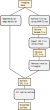
\includegraphics[height=15cm]{images/fiber_creation/scheme_preprocessing.pdf}%
  \caption{Workflow of generating a surface representation of the muscle and tendons from imaging data. Operations and intermediate results are shown as gray and yellow boxes, respectively. Two alternatives are given by the two branches. On the left, the imaging data is automatically processed to directly retrieve points on the surface of the muscle. The right branch achieves the same with three steps of which the first one involves manual adjustments. At the end, a spline surface smooths the collected data from both possibilities to yield the resulting surface representation.}%
  \label{fig:scheme_preprocessing}%
\end{figure}%

\subsection{Data Source}
Anatomic images provide the basis for the extraction of muscle geometries.
Our used data set originates from the Visible Human Project \cite{visible_human_male} of 
the United States National Library of Medicine. 
The project has published anatomic images derived from a male cadaver, among other data sets.
The data, known as \say{Visible Human Male}, were published in 1994.
Colored images of transversal cross sections were obtain by cryosectioning.
A total of \num{1871} images with dimensions of \num{2048} by \num{1216} pixels and 24 bit color depth visualize the whole human body. Parts of the upper arms are contained in approximately 500 of these images. The size of a pixel is \SI{0.33}{\milli\meter} in transversal direction and \SI{1}{\milli\meter} in axial direction. The size of the complete set of JPEG compressed images is \SI{772}{\mega\byte}. Cropping and selecting the relevant portions of the upper arm extracts a dataset with the size of \SI{35}{\mega\byte}.

An extract of an image of the upper arm is given in \cref{fig:vhp_image}. 
The location of biceps and triceps brachii muscles can be identified in the dark red tissue. For the biceps, the two muscle heads are visible, separated by the bright diagonal line from bottom left to top right. For the triceps, at least two of the three heads can be identified. The blue background is colored frozen gelatin that was needed during cryosection to stabilize the arms.

\begin{figure}%
  \centering%
  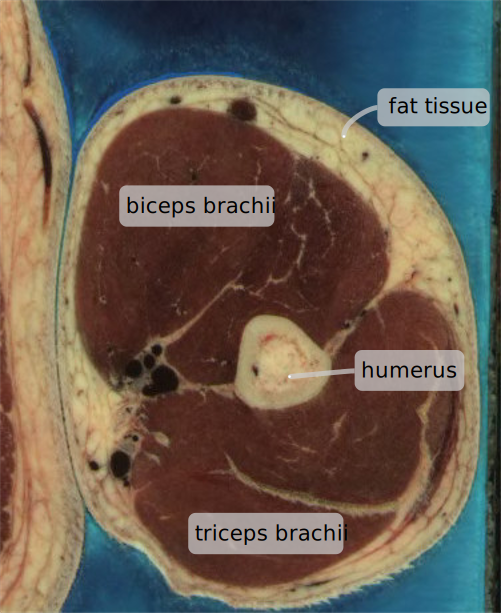
\includegraphics[height=10cm]{images/fiber_creation/vhp.png}% 0483
  \caption{Exemplary extract of image number 483 from the Visible Human Male. A transversal slice of the left upper arm is shown as seen from the bottom. The biceps and triceps muscles as well as the humerus bone can be identified. }%
  \label{fig:vhp_image}%
\end{figure}%

\subsection{Automatic Surface Extraction}
This section outlines the automatic algorithm to obtain the muscle surface from the Visible Human Male data set. The scheme corresponds to the left branch in \cref{fig:scheme_preprocessing}. The algorithm was implemented in a Python script as part of the Bachelor thesis of Kusterer \cite{Kusterer} that was supervised by me.
The algorithm is capable of extracting muscle and bone geometries from the mentioned imaging dataset.

At first, the color values in the images are used to segment the pixels into muscle tissue, surrounding tissue and skeletal structure. The algorithm traverses the selected and cropped relevant parts of the images. For example, to consider the biceps muscle, the image region of pixels coordinates $(x,y)$ with $x \in [1300,1720] $ and $ y\in[1030,1720]$ are considered in the images with numbers 284 to 778. 

For every such part of an image, pixels that match a certain range in the RGB color space are marked and categorized. The categories are muscle tissue and, for demonstration, also bone tissue. The corresponding color ranges are given in \cref{tab:color_ranges}.

The color based classification does not succeed everywhere as the white shade corresponds not only to bone material but also to fat and other tissue. Therefore, the algorithm removes artifacts located near the outer gelatine from the set of pixels that was categorized as bone. 

\begin{table}
  \centering%
  \begin{tabular}{l|lll}
    \hline
    & red & green & blue\\
    \hline
    muscle & $60 - 100$& $30-75$   & $15-60$\\
    bone   & $145-255$ & 1$35-205$ & $60-160$\\
    \hline
  \end{tabular}
  \caption{Ranges in the RGB color space to identify pixels of muscle and bone segments. The numbers correspond to 24 bit colors with the range $[0,255]$ for every color channel.}%
  \label{tab:color_ranges}%
\end{table}

Exemplary results for image number 483 are given in the left column of \cref{fig:extraction}.
It can be seen that the marked regions for muscle and bone have gaps in the interior resulting from differently colored tissue inside muscles and bones. On some images, the set of pixels also includes small objects outside the actual muscle and bone regions.

To reduce the gaps and small objects, the morphological operations \emph{closing} and \emph{opening} are applied on the data. These operations consist of \emph{dilation} and \emph{erosion} steps. Both are pixel based operations that traverse the dataset and for every pixel consider a window of $3\times 3$ pixels centered at the current position. Dilation picks the maximum value and erosion the minimum value from this window and assigns it as the pixel's value in a new image. In our case, values of zero and one correspond to non-categorized and categorized pixels, respectively.

Closing consists of dilation followed by erosion and closes small gaps or holes in the marked objects. Opening consists of erosion followed by dilation and removes small artifacts outside the actual bone and muscle areas. It was found effective to perform both dilation and erosion twice in sequence to yield good results containing almost no more holes nor unwanted small objects.

Next, the algorithm determines the contours of all regions with marked pixels. This leads to lines with a width of one pixel that enclose the muscle and bone areas. The right column of \cref{fig:extraction} shows the results after this step. It can be seen that numerous gaps have been closed by the morphological operations. In some images, as in the considered example, the muscle area gets split into multiple smaller enclosed regions, which is not desired. However, proper contours of the biceps are found in the majority of images. 

\fboxsep=0mm   % padding thickness
\fboxrule=1pt   % border thickness
\begin{figure}%
  \centering%
  \fcolorbox{black}{black}{\includegraphics[height=7cm,trim=0 0 0 6cm, clip]{images/fiber_creation/extraction_segmentation_482.png}}\quad%
  \fcolorbox{black}{black}{\includegraphics[height=7cm,trim=0 0 0 4cm, clip]{images/fiber_creation/extraction_contour_482.png}}\vspace*{5mm}\\
  \fcolorbox{black}{black}{\includegraphics[height=7cm,trim=0 0 0 6cm, clip]{images/fiber_creation/extraction_bone482.png}}\quad%
  \fcolorbox{black}{black}{\includegraphics[height=7cm,trim=0 0 0 6cm, clip]{images/fiber_creation/extraction_surface_bone482.png}}%
  \caption{Intermediate steps of the algorithm to determine surface geometry of muscles and bones. The left columns shows pixels from the image in \cref{fig:vhp_image} that were categorized to be muscle tissue (top) and bone material (bottom). The right column shows a later step in the algorithm, where the surface of muscle (top) and bone (bottom) is estimated.}%
  \label{fig:extraction}%
\end{figure}%

In the next step, a single contour for each of muscle and bone is obtained in every image. If there are multiple contours per image, the one that is located the most in upper right location within the image is selected for the muscle. If all contours in an image are shorter than 20 pixels, this is an indication for bad segmentation quality and the whole image gets discarded.

The result is a set of contours for muscle and bone in the cross-sectional planes of the images. Combining these, we get a point cloud in 3D space that approximates the surface of the biceps muscle and the surfaces of the considered bones humerus, ulna and radius. Using these points, a spline surface can be fitted and subsequently triangulated. Resulting surfaces for the biceps and humerus bones are shown in \cref{fig:extraction_result}.
%
\begin{figure}%
  \centering%
  \begin{subfigure}[t]{0.48\textwidth}%
    \centering%
    \includegraphics[height=7cm]{images/fiber_creation/extraction_biceps.png}%
    \caption{Surface of the biceps brachii muscle. At the right side of the muscle, the groove of the humerus bone can be seen.}%
    \label{fig:extraction_result_biceps}%
  \end{subfigure}
  \begin{subfigure}[t]{0.48\textwidth}%
    \centering%
    \includegraphics[height=7cm]{images/fiber_creation/extraction_humerus00.png}%
    \caption{Surface of the humerus}%
    \label{fig:extraction_result_humerus}%
  \end{subfigure}    
  \caption{Resulting surfaces of biceps and humerus bone obtained by the automatic surface extraction algorithm.}%
  \label{fig:extraction_result}%
\end{figure}%

The runtime for the algorithm is \SI{121}{\minute} on a AMD Ryzen 5 1600 processor with 6 cores, 3.2 GHz and \SI{16}{\giga\byte} RAM, of which a maximum of \SI{2}{\giga\byte} was used at maximum. Because processing of the images can be done in parallel, the runtime can be reduced to approximately half (\SI{62}{\minute}) using 2 threads and to a quarter (\SI{30}{\minute}) using 6 threads.

The advantage of the presented algorithm is that the outcome solely depends on the imaging data and, thus, no modeling error by manual approximation of the geometry occurs. For example, the obtained surfaces of biceps and humerus geometrically fit perfectly into each other. Intermediate steps are stored as black and white images. By editing these between the steps of the algorithm, manual tweaking is possible and can be used to increase the quality of the results.

A disadvantage is that the algorithm relies on color information in the imaging data to differentiate between muscle and other tissue. Because the involved tissue has similar colors, these differences are often small. Furthermore, the color ranges need to be determined experimentally. Therefore, the algorithm is not very robust with respect to image noise and needs adjustments when it should be used to extract other muscles. Expert knowledge about the location and shape of human muscles cannot be used easily to improve the results of the algorithm.

An alternative approach is to manually segment the imaging data and construct surfaces with the help of a tool. This approach is described in the following section.

\subsection{Manually Guided Surface Extraction}\label{sec:surf_extr}

Manually guided segmentation can be done using the \emph{MAP client} of the Musculoskeletal Altas Project (MAP) \cite{mapclient}. This application allows to create and execute a workflow to achieve data processing and simulation tasks. In a graphical window, the user can place and connect various workflow steps. When executing the workflow, each step shows a dialog where the required configuration can be entered or the operations can be performed on a visual presentation of the data at this workflow stage. 

Possible workflow steps include source and sink operations such as reading image data and writing meshes. Imaging data such as the 2D images from the Visual Human Male can be visualized in a 3D representation. The user can place points in the 3D space and try to match borders of the muscles and structures to extract from the data.
Further workflow steps allow to create meshes of predefined geometrical shapes, such as cubes and cylinders and merge them into a common mesh. These meshes can be fitted to point clouds of user defined points. This is done by a least squares approach minimizing the distances between user created points and the mesh surface. Details can be found in \cite{Fernandez2018}.

The MAP client has a plugin architecture and allows to create new workflow steps. It imports features from OpenCMISS, especially data processing formats and tools from OpenCMISS Zinc. Meshes can be created with 3D cubic Hermite elements that allow a high geometric modeling flexibility with a low number of nodes. Such meshes are stored in the OpenCMISS file format of \code{exnode} and \code{exelem} files.

As a result, meshes of individual muscles or the whole human organism can be created. \Cref{fig:vhp_geometry} shows meshes that were create from the cryosectioning data of the Visible Human Male. In \cref{fig:vhp_total} almost the whole body has been extracted. In \cref{fig:vhp_detail}, the mesh consisting of cubic Hermite elements is visualized. A relatively coarse mesh width suffices to model a smooth surface of the body. When exported in the exfiles format from the MAP client, the data can be visualized, e.g., using \emph{cmgui}, the visualization tool of OpenCMISS Zinc.

\begin{figure}%
  \centering%  
  \begin{subfigure}[t]{0.48\textwidth}%
    \centering%
    \includegraphics[height=10cm]{images/fiber_creation/skin00.png}%
    \caption{Mesh of the trunk and limbs, the surface has been triangulated for visualization.}%
    \label{fig:vhp_total}%
  \end{subfigure}
  \quad
  \begin{subfigure}[t]{0.48\textwidth}%
    \centering%
    \includegraphics[height=7cm]{images/fiber_creation/elements4_red.png}%
    \caption{Detail view of part of the right upper arm and the trunk with orange nodes and edges of a cubic Hermite element mesh.}%
    \label{fig:vhp_detail}%
  \end{subfigure} 
  \caption{Mesh of the Visible Human Male from the Visible Human Project.}%
  \label{fig:vhp_geometry}% 
\end{figure}%

The mesh width of the meshes obtained using the MAP client was chosen such that the surface fitting yielded good results. The meshes are not necessarily ready for use in a simulation, especially if a  high mesh resolution is desired. 
Apart from the mesh width also the type of elements can be different than what is needed for a Finite Element simulation. Our goal is to obtain meshes with linear or quadratic Lagrange elements with configurable mesh widths for the specified upper arm muscles, such as the biceps brachii.

Therefore, the next step of the workflow, as visualized by the right branch of \cref{fig:scheme_preprocessing}, is to transform the volume mesh into a surface mesh which then can be used as start for further meshing. The further meshing steps are visualized in \cref{fig:biceps_processing}. The start is the Hermite mesh shown in the left-most image.

\begin{figure}%
  \centering%
  \includegraphics[height=10cm]{images/fiber_creation/exfile_red.png}\quad%
  \includegraphics[height=10cm]{images/fiber_creation/biceps23.png}%
  \includegraphics[height=10cm]{images/fiber_creation/biceps22.png}%
  \includegraphics[height=10cm,trim=-2cm 0 0 -2cm, clip]{images/fiber_creation/splines00.png}%
  \caption{Processing the geometry of the biceps brachii muscle. From left to right: mesh with cubic Hermite elements, STL mesh with inside triangles, STL surface mesh where triangles lying inside have been removed, Spline surface of the muscle belly.}%
  \label{fig:biceps_processing}%
\end{figure}%

The Hermite elements can be triangulated and stored as an STL file using the tool \mbox{\code{cmgui}.} This process triangulates the non-planar faces of all Hermite elements. This leads to a dataset with triangles both on the surface and in the inside of the volume, as can be seen in the second image of \cref{fig:biceps_processing}. At this stage, the use of the MAP and OpenCMISS related tools is finished and further processing steps are performed using tools from \opendihu{} that we developed on our own.

A Python script removes the triangles in the inside of the volume. The detection whether a triangle is inside the volume is done by casting four rays from the center of gravity of the triangle and determining if the rays intersect any other triangles. The rays have directions $(x,y,z) = (\pm1,\pm1,\frac13)$, where the $z$ axis is oriented along the muscle and the $x$ and $y$ axes are oriented in radial direction. The ray-triangle intersection is done using the fast Möller-Trumbore algorithm \cite{ray-triangle}. For every ray, all triangles are checked.
Only if all four rays intersect at least one more triangle, the starting triangle is considered to be inside the volume and subsequently removed from the dataset. 

This algorithm has a quadratic time complexity $\O(n^2)$ in the number of triangles $n$. It could be improved by organizing the triangles in a spatially adaptive data structure, such as an octree. However, since this preprocessing step has to be performed only once for a given geometry the runtime is not a concern and there is no need for such optimization.

The result of this operation is a triangulated surface, shown in the third image of \cref{fig:scheme_preprocessing}. The next step is to create a Spline surface of the muscle belly, as shown in the right-most image of \cref{fig:scheme_preprocessing}. This is described in the next two sections.

\subsection{Introduction of Spline Surfaces}\label{sec:nurbs}
The surface representation of the muscle could be obtain from either the left or the right branch of the preprocessing workflow in \cref{fig:scheme_preprocessing}. The surface is given by a point cloud or a number of triangles. To remedy eventual outliers or unphysiological sharp edges from the segmentation, a Spline surface is fitted to the data. This leads to a smooth surface representation and later to a better conditioned Finite Element mesh in the simulation. However, this step is optional. It is also possible to use the surface triangulation from previous section \ref{sec:surf_extr} for the meshing algorithm in the next section \ref{sec:ser_alg_meshes}.

The surfaces uses Nonuniform Rational B-splines (NURBS). A NURBS surface is a generalization of a B-spline surface. From a modeling point of view, B-spline surfaces have three advantages. First, the B-spline surface can be constructed with given smoothness properties.  Second, the definition of a particular B-spline surface builds on geometric information, which simplifies their creation. More specifically a control polygon mesh in the 3D space is defined. Its convex hull is guaranteed to contain the surface. Third, the geometric parameters of a B-spline surface have only local impacts on the shape of the surface. This allows a B-spline surface of a fixed, low polynomical degree to approximate point clouds with any number of points without loosing approximation quality.

A limitation of B-spline surfaces is that circular and spherical shapes cannot be represented. This limitation is overcome by NURBS surfaces. NURBS surfaces are defined as the perspective projection into 3D space of a B-spline surface in 4D space.

The mathematical description is given in this section, following the notation of \cite{piegl2012nurbs}. The building blocks are the B-spline basis functions of polynomial degree $p$. Given a knot vector 
%
\begin{align*}
  \Xi = (\xi_1, \xi_2, \dots, \xi_k), \quad \text{with } a=\xi_1 \leq \xi_2 \leq \cdots \leq \xi_k = b,
\end{align*}
%
the $i$th B-spline basis function $N_{i,n}$ of degree $n$ is defined recursively starting with the piecewise constant function $N_{i,0}$ for $n=0$,
%
\begin{align*}
  N_{i,0}(\xi) = \begin{cases} 
    1 \, &\xi_i \leq \xi < \xi_{i+1},\\[2mm]
    0 &\text{else},
  \end{cases}
\end{align*}
and using the following relation to define the functions of higher degree, $n > 0$,
\begin{align*}
  N_{i,n}(\xi) = \dfrac{\xi - \xi_i}{\xi_{i+n} - \xi_i} N_{i,n-1}(\xi) + \dfrac{\xi_{i+n+1} - \xi}{\xi_{i+n+1} - \xi_{i+1}} N_{i+1,n-1}(\xi), \quad i > 0.
\end{align*}
Because neighbouring entries in the knot vector can be equal, the fraction $0/0$ can occur. In this case, $0/0 := 0$ is defined.

A B-spline curve $\bfC \in \R^d$ of polynomial degree $p$ is defined as
%
\begin{align*}
  \bfC(u) = \s{i=1}{l}N_{i,p}(u)\,\bfP_i, \quad u \in [a,b].
\end{align*}
%
The coefficients $\bfP_i \in \R^d, i=1, \dots, l$ to the basis functions $N_{i,p}$ are called \emph{control points} and define the control polygon. The number $l$ of basis functions and control points is determined from the number of knots $k$ in an open knot vector and the polynomial degree $p$ as $l = k-p-1$.

The number of equal entries in series in the knot vector is the \emph{multiplicity} of the respective knot value. Usually \emph{open} knot vectors $\Xi$ are used where the first and the last knot occur with a multiplicity of $p+1$.
This make the first and last points of the B-spline curve coincide with the control polygon, $\bfC(a) = \bfP_1$ and $\bfC(b) = \bfP_l$.

The multiplicities of the knots in the knot vector encode information about the smoothness of the B-spline curve. If the knot value $\hat{\xi}$ has a multiplicity of $m$, the B-spline curve will be $(p-m)$ times continuously differentiable at $\bfC(\hat{\xi})$.
% This can be seen from the fact that there exist $m$ basis functions with a support that begins at $\hat{\xi}$.

An exemplary B-spline curve is shown in \cref{fig:bspline_curve}. It uses a \emph{non-uniform} knot vector for polynomial degree $p=3$, where the differences $\xi_{i+m} - \xi_i$ between neighbouring knot values vary. The effect of different multiplicities can be seen. The multiplicity $m=p=3$ places the knot on the respective control point, as for $\xi=49$ in the example. The multiplicity $m=p-1=2$ places the knot on the control polygon, as in the example at $\xi=10$. A lower multiplicity $m < p-1$ does not yield a higher smoothness and in turn does not force the curve on the control polygon. It can also be seen that the B-spline curve stays inside the convex hull of the control polygon which is a property of B-spline curves \cite{piegl2012nurbs}.

\begin{figure}%
  \centering%
  \def\svgwidth{8cm}%
  \input{images/fiber_creation/bspline_curve.pdf_tex}%
  \caption{Exemplary B-spline curve (red) of degree $p=3$ for the knot vector $\Xi = (0,0,0,0,7,10,10,49,49,49,50,50,50,50)$, control points (blue) and control polygon (black).
  Positions of the curve $\bfC(\xi_i)$ at the knots $\xi_i$ are indicated by the red squares and the knot value $\xi$ and its multiplicity $m$ is given. The effect of moving one control point is shown in green.}%
  \label{fig:bspline_curve}%
\end{figure}%
%
The effect of moving one of the 10 control points is visualized with green color in \cref{fig:bspline_curve}.
The B-spline basis function $N_{i,p}$ has a local support of $S=(\xi_i,\xi_{i+p+1})$. Consequently, only the corresponding part of the curve, $\bfC(\xi)$ for $\xi \in S$ changes.

A B-spline surface $\bfS$ is given by the tensor product of two B-spline curves :
\begin{equation}\label{eq:bspline_surface}
  \begin{array}{lll}
    \bfS(u,v) = \s{i=1}{l^{(1)}}\s{j=1}{l^{(2)}} N^{(1)}_{i,p^{(1)}}(u)\,N^{(2)}_{j,p^{(2)}}(v)\, \bfP_{i,j}.
  \end{array}
\end{equation}
Here, we have two polynomial degrees $p^{(1)}$ and $p^{(2)}$, the ansatz functions $N^{(1)}$ and $N^{(2)}$ with number of ansatz functions $l^{(1)}$ and $l^{(2)}$ are constructed from corresponding knot vectors, each.

NURBS, B-spline curves and surfaces are formulated using \emph{homogeneous coordinates}. Every point in Cartesian coordinates $(x,y,z) \in \R^3$ has a set of homogeneous coordinates $(\tilde{x},\tilde{y},\tilde{z},w)=(x\,w,y\,w,z\,w,w)$. Thus, the Cartesian coordinates can be obtain from the homogeneous coordinates by the \emph{perspective division}, i.e., dividing all but the last coordinate by the weight $w$.

A NURBS surface is given by the same definition as the B-spline surface in \cref{eq:bspline_surface} except that the control points $\bfP_{i,j} \in \R^3$ are enriched with scalar weights $w_{i,j}$ and, thus, replaced by $(\bfP_{i,j}, w_{i,j}) \in \R^4$. The resulting surface $\bfS$ is given in homogeneous coordinates. Executing the perspective division yields the form:
%
\begin{align*}
  &\bfT(u,v) = \s{i=1}{l^{(1)}}\s{j=1}{l^{(2)}} R_{i,j}(u,v) \,\bfP_{i,j},\\[4mm]
  &\text{with } R_{i,j}(u,v) = \dfrac{N_{i,p^{(1)}}(u)\,N_{j,p^{(2)}}(v)\,w_{i,j}}{\s{r=1}{l^{(1)}}\s{s=1}{l^{(2)}} N_{r,p^{(1)}}(u)\,N_{s,p^{(2)}}(v)\,w_{r,s}}.
\end{align*}
The new rational basis functions $R_{i,j}$ and the possibly non-uniform knot vectors give rise to the name Non-Uniform Rational B-spline surface (NURBS).

\subsection{Fitting a Spline Surface to the Muscle Geometry}
In order to find a NURBS surface for the given triangulated surface of a muscle, at first, the part of the geometry corresponding to the tendons is removed such that the resulting triangles model only the surface of the muscle belly. The resulting belly has a length of \SI{12.8}{\mm}.

Then, twelve cross sections are extracted from the surface triangles. In result, we get twelve horizontal circumferential rings. On each ring, 9 equidistant points are determined. The first point is appended after the last point in every ring, such that in total we obtain a grid of $10 \times 12$ points. 

Then, the least squares surface approximation algorithm by \cite{piegl2012nurbs} is used to fit a NURBS surface to the points. The implementation of the algorithm is given by the NURBS-Python (geomdl) library. Polynomial degrees of $p^{(1)} = 3$ and $p^{(2)}=2$ are used where the first dimension corresponds to the cross-sectional direction of the muscle. The knot multiplicity is chosen as $m=1$ for both coordinate directions. In result, we obtain a two times respective one times continuously differentiable surface in $u$ and $v$ direction. 
The resulting NURBS surface and the control polygon is visualized in \cref{fig:biceps_splines_control_points}. Note that the control polygon is different from the grid of points against which the surface is fitted.
%
\begin{figure}%
  \centering%
  \includegraphics[width=0.35\textwidth]{images/fiber_creation/splines01red.png}%
  \caption{Fitted NURBS surface of the biceps muscle (red) and the control polygon (orange).}%
  \label{fig:biceps_splines_control_points}%
\end{figure}%

\Cref{fig:biceps_splines_wrong} shows the result of this approach in more detail. It can be seen that the surface is non-differentiable and has a kink at the seam line where the first and last points of each ring meet. The reason for this is that the surface fitting algorithm does not pose any conditions on the tangents at the edges of the fitted NURBS surface.  Thus, the tangents mismatch.

Since no implementation of a fitting algorithm specifically for a tubular NURBS surface with periodicity in tangential direction is available, we develop a different remedy. We modify the point grid that is used for the surface fitting. The series of 9 equidistant points on each ring is replicated twice and the first point is again added as the last point. This leads to a grid of $(3\cdot 9+1) = 28 \times 12$ points which wrap around the muscle volume in cirumferential direction three times. The NURBS surface fitting algorithm is applied on this grid. The resulting NURBS surface also wraps around the muscle three times with the two ends being again not properly fitting to each other. From these three wraps, the middle one is extracted. In the biceps example, this corresponds to restricting the NURBS surface $\bfT(u,v)$ from $(u,v) \in [0,1]^2$ to $(u,v) \in [0.4,0.733]\times [0.1]$.

The result is depicted in \cref{fig:biceps_splines_seam} and it can be seen that the tangents now match very well between the two sides of the NURBS surface. Additionally, the comparison with the inital approach in \cref{fig:biceps_splines_wrong} shows that an artifical bulge at the top of the muscle in the perspective of the visualization is removed. The overall shape of the muscle now looks smoother and more natural. Also, a comparison with the result of the automatic algorithm given in \cref{fig:extraction_result_biceps} shows that the results of our new approach are smoother.

The generated tubular surface has two holes at the top and bottom which prevent it from being an enclosing surface to the muscle belly volume. The borders of these holes each lie in a plane and, thus, the missing surfaces are treated as being planar during the subsequent creation of the 3D meshes.
%
\begin{figure}%
  \centering%
  \begin{subfigure}[t]{0.48\textwidth}%
    \centering%
    \includegraphics[height=8cm]{images/fiber_creation/splines_wrong00.png}%
    \caption{First approach with $10 \times 12$ points. The kink at the seam line along the muscle is clearly visible.}%
    \label{fig:biceps_splines_wrong}%
  \end{subfigure}
  \quad
  \begin{subfigure}[t]{0.48\textwidth}%
    \centering%
    \includegraphics[height=8cm]{images/fiber_creation/splines_seam00.png}%
    \caption{Second, improved approach with $28 \times 12$ points. It can be seen that the tangent at the seam line matches very well.}%
    \label{fig:biceps_splines_seam}%
  \end{subfigure}
  \caption{Fitted NURBS surface of the biceps muscle, triangulated for visualization purposes.}%
  \label{fig:biceps_splines}%
\end{figure}%
%
\section{Serial Algorithm to Create Muscle and Fiber Meshes}\label{sec:ser_alg_meshes}
Next, a 3D mesh for the muscle volume and 1D meshes for muscle fibers need to be generated from the surface representation described in the last sections. In this section, first an algorithm for the 3D mesh is described. Then, a second algorithm that reuses results from the first algorithm is presented which generates one dimensional meshes for muscle fibers. Both algorithms are executed in serial. A derived algorithm that can run in parallel and, thus, can handle larger datasets on a distributed memory hardware is given in the next section, \cref{sec:parallel_algorithm}.

The steps of a serial algorithm for the generation of a 3D mesh are given in \cref{alg:serial_algorithm_1}. Input is the set of triangles at the tubular surface of the muscle. The tubular surface is oriented along the $z$ axis. In the following descriptions the muscle in considered to be oriented upright such that the $z$ axis points in vertical direction towards the top. The borders at bottom and top have a constant $z$ coordinate.
%
\begin{algorithm}
  \begin{algorithmic}[1]%
    \Procedure{Create\_3D\_mesh}{}
    \Require Triangulated tubular surface
    \Ensure Structured 3D volume mesh
    \Statex
    \State Slice geometry           \label{alg:1.1}
    \State Triangulate 2D slices      \label{alg:1.2}
    \State Compute harmonic maps $u, v$      \label{alg:1.3}
    \State Construct regular grid in parameter space and map to slices            \label{alg:1.4}
    \State Form 3D quadrilateral elements between the 2D slices’ meshes   \label{alg:1.5}
    \EndProcedure
  \end{algorithmic}%
  \caption{Serial algorithm for generation of 3D meshes}%
  \label{alg:serial_algorithm_1}%
\end{algorithm}%

\subsection{Slicing of the Geometry}\label{sec:slicing_of_the_geometry}
The first step in line \algref{alg:serial_algorithm_1}{alg:1.1} slices the geometry. This means that horizontal \emph{slices} of the cross-sectional area are extracted from the surface mesh. First, the muscle is divided into equidistant positions $z_i, i=1,\dots,n$ along the $z$-axis where the slices are to be extracted. As can be seen in \cref{fig:serial_alg_0}, $n=13$ $z$ coordinates are selected. Next, for every position $z_i$, all surface triangles $T_j$ that intersect the plane $Z_i = \{\bfp=(x,y,z) \mid z=z_i$\} are considered and the intersection lines $P = T_j \cap Z_i$ are computed. The method of computing plane-triangle intersection is described in the following.

Given is a triangle $T$ with points $\bfp^{1},\bfp^2,\bfp^3 ∈ \R^3$ and a value $\hat{z}$, the wanted result is the set of points $P = T ∩ \{\bfp = (\bfp_x,\bfp_y,\bfp_z) \mid \bfp_z=\hat{z}\}$ which corresponds to a line segment $\overline{\bfp^a\bfp^b}$. 

We describe the points in the triangle by two barycentric coordinates $\xi_1$ and $\xi_2$ as
\begin{equation}\label{eq:barycentric_triangle}
  \begin{array}{lll}
    \bfp(ξ_1,ξ_2) = (1-ξ_1-ξ_2)\,\bfp^{1} + \xi_1\,\bfp^{2} + \xi_2\,\bfp^{3},  \\[4mm]
    \text{with }\xi_1+\xi_2 \leq 1, \quad 0 \leq \xi_1,\xi_2 \leq 1.
  \end{array}
\end{equation}
By letting $\bfp_z(ξ_1,ξ_2) = \hat{z}$ we calculate the equation for the line segment $\overline{\bfp^a\bfp^b}$ in barycentric coordinates to be
\begin{equation*}
  \begin{array}{lll}
    ξ_1 = m\cdot ξ_2 + c,\quad
    m = -\dfrac{\bfp_z^{3} - \bfp_z^{1}}{\bfp_z^{2} - \bfp_z^{1}}, \quad c = \dfrac{\hat{z} - \bfp_z^{1}}{\bfp_z^{2} - \bfp_z^{1}}, \quad \bfp_z^2 \neq \bfp_z^1.
  \end{array}
\end{equation*}
For $\bfp_z^1 = \bfp_z^2 \neq \bfp_z^3$ we swap $\bfp_z^2$ and $\bfp_z^3$.

%
%  # x(xi1,xi2) = (1-xi1-xi2)*x^{1} + xi1*x^{2} + xi2*x^{3},  xi1+xi2 <= 1, 0 <= xi1,xi2 <= 1
%  # x_3(xi1,xi2) = z_value  =>  (1-xi1-xi2)*x^{1} + xi1*x^{2} + xi2*x^{3} = z_value
%  #                         =>  xi1*(x^{2} - x^{1})  +  xi2*(x^{3} - x^{1})  =  z_value - x^{1}
%  #                         =>  xi2 = ((z_value - x^{1}) - xi1*(x^{2} - x^{1})) / (x^{3} - x^{1})
%  #                         =>  xi2 = (z_value - x^{1})/(x^{3} - x^{1}) - xi1 * (x^{2} - x^{1})/(x^{3} - x^{1})
%  #                         =>  xi1 = (z_value - x^{1}) / (x^{2} - x^{1})  - xi2 * (x^{3} - x^{1}) / (x^{2} - %x^{1}) 
We consider the three sides $\overline{\bfp^1\bfp^2}, \overline{\bfp^2\bfp^3}$ and $\overline{\bfp^3\bfp^1}$ of the triangles and check which of them is intersected by the $z=\hat{z}$ plane.
\begin{enumerate}
\item On the triangle side $\overline{\bfp^1\bfp^2}$, the condition $ξ_2 = 0$ holds and the side intersects the plane 
at $\bfp(c,0)$ 
iff $0 \leq c \leq 1$. 
\item On the triangle side $\overline{\bfp^1\bfp^3}$, we have the condition $ξ_1 = 0$ and the side intersects the plane 
at $\bfp(0,-c/m)$ 
iff $m\neq 0 \wedge 0 \leq -c/m \leq 1$. 
\item The third triangle side $\overline{\bfp^2\bfp^3}$ is intersected for $ξ_1=(c+m) / (1+m)$
at $\bfp(ξ_1,1-ξ_1)$ 
iff ${m \neq -1 \wedge 0 \leq (c+m)/(1+m) \leq 1}$.
\end{enumerate}
If two of these three conditions for intersection of the triangle sides are met, there is an intersecting line segment $\overline{\bfp^a\bfp^b}$ with $\bfp^a \neq \bfp^b$ and the two intersection points $\bfp^a$ and $\bfp^b$ on the triangle sides need to be computed. The case $\bfp^a = \bfp^b$ and the case where two or more of the triangle points are lying on the $z=\hat{z}$ plane are handled separately.

After the presented computations are performed for all planes $Z_i$ and all triangles $T_j$, we have a number of line segments that form a geometric \say{ring} for each $z$ plane. The line segments are ordered according to their adjacency and a counter-clockwise orientation with respect to the $z$ axis is ensured.
The length of each ring is computed. A number $m=16$ of equidistant points is selected on each ring.

Because the selected points on the rings are later used as border points of the volume mesh their position relative to each other should be in a tidy manner. When viewing the points on the surface in a $x-z$ or $y-z$ projection, they should approximately form a uniform regular grid like in the result in \cref{fig:serial_alg_0}. With given rings and number $m$ of equidistant points per ring, only the position of one point per ring is not yet fixed. To close the definition, we formulate a first condition that relates the point positions of two neighbouring rings and a second condition for one point at the bottom-most ring.

The first condition should ensure that the point positions on neighbouring rings are as similar as possible. This is done by minimizing the distance between the one point on every ring that is fixed first.
In the algorithm, the $z$ planes are traversed from bottom to top. 
The first point $\tilde{\bfp}_{i,0}$ on a ring at $z=z_i$ is determined from the first point $\tilde{\bfp}_{i-1,0}$ of the previous ring at $z=z_{i-1}$ as the one with the minimal distance $|\tilde{\bfp}_{i,0} - \tilde{\bfp}_{i-1,0}|$. 
Thus, the searched point $\tilde{\bfp}_{i,0}$ has the property that the line between $\tilde{\bfp}_{i,0}$ and $\tilde{\bfp}_{i-1,0}$ and the tangent of the ring are perpendicular.

Given any point $\bfp$ on the ring at $z_i$ and the tangent vector $\bfu$ at this point, we can project the connection vector $\bfv$ from $\bfp$ to the start point $\tilde{\bfp}_{i-1,0}$ of the previous ring, $\bfv = \tilde{\bfp}_{i-1,0} - \bfp$, onto the tangent $\bfu$. This leads to the plumb foot point $\bfp_0$ by the computation
\begin{equation*}
  \begin{array}{lll}
    \bfp_0 = \bfp + t\,\bfu \quad \text{with }t = \dfrac{\bfv \cdot \bfu}{|\bfu|^2}.
  \end{array}
\end{equation*}
Performing this calculation for every line segment $u$ on a ring allows to select the plumb foot $\bfp_0$ with the smallest distance to the start point $\tilde{\bfp}_{i-1,0}$ of the previous ring to be the start point $\tilde{\bfp}_{i,0}$ of the current ring. This is the point that fulfills the first condition.

With this first condition all points are only fixed relative to each other. The definition of one point, the start point $\tilde{\bfp}_{0,0}$ of the bottom-most ring, is missing. The second condition fixes this point by a prescribed plane at $x = \hat{x}$ and selects $\tilde{\bfp}_{0,0}$ such that its $x$ coordinate lies in this plane. From the (usually two) points that meet this condition, the one with lower $y$ coordinate is selected. The actual value of $\hat{x}$ is determined experimentally such that the resulting point positions are visually uniform. Not every value leads to a good result because of the shape of the biceps muscle, especially the groove where the humerus bone is located.

The resulting grid of points on the biceps surface is visualized in \cref{fig:serial_alg_0}. It can be seen that all points of the same ring have the same $z$ coordinate. By connecting neighbouring points horizontally and vertically, a regular grid can be formed. This overall grid in this $x-z$ perspective view looks relatively uniform, e.g., compared with the gray surface triangulation mesh of the biceps geometry. The spacing between the points is lower at the top and bottom of the muscle because of the smaller circumference at these locations.

%
\begin{figure}%
  \centering%
  \begin{subfigure}[t]{0.48\textwidth}%
    \centering%
    \includegraphics[height=10cm]{images/fiber_creation/serial_alg_0.png}% [trim=left bottom right top, clip]
    \caption{Extracted border points (blue) on the biceps surface mesh (gray). This is the result of line \algref{alg:serial_algorithm_1}{alg:1.1}.}%
    \label{fig:serial_alg_0}%
  \end{subfigure}
  \quad
  \begin{subfigure}[t]{0.48\textwidth}%
    \centering%
    \includegraphics[height=10cm]{images/fiber_creation/serial_alg_3.png}%
    \caption{The generated triangulation of the slices (left) and the image $\bfy(\bfx)$ of the triangulation under the harmonic map (right). This figure shows the result of lines \algref{alg:serial_algorithm_1}{alg:1.2} and \algref{alg:serial_algorithm_1}{alg:1.3}.}%
    \label{fig:serial_alg_3}%
  \end{subfigure}\\
  \centering%
  \begin{subfigure}[t]{0.49\textwidth}%
    \centering%
    \includegraphics[height=10cm]{images/fiber_creation/serial_alg_4_orange.png}%
    \caption{Grid in parameter space (right) and muscle domain (left), result after line \algref{alg:serial_algorithm_1}{alg:1.4}.}%
    \label{fig:serial_alg_4}%
  \end{subfigure}
  \hfill{}
  \begin{subfigure}[t]{0.4\textwidth}%
    \centering%
    \includegraphics[height=10cm]{images/fiber_creation/serial_alg_8_orange.png}%
    \caption{3D elements formed by connecting the slices, result after line \algref{alg:serial_algorithm_1}{alg:1.5}.}%
    \label{fig:serial_alg_8}%
  \end{subfigure}
  \caption{Steps of the serial algorithm, \cref{alg:serial_algorithm_1}, executed directly on the surface mesh of the biceps muscle (not the B-spline surface).}%
  \label{fig:serial_alg}%
\end{figure}%
%

\subsection{Triangulation of the Slices}\label{sec:triangulation_of_the_slices}
The points of each ring enclose a planar, polygonal surface, a \emph{slice} $S_M$ of the muscle.
The next step in the algorithm, line \algref{alg:serial_algorithm_1}{alg:1.2}, is to triangulate the extracted slices, i.e. construct triangles that decompose the polygons. The result of this step is visualized at the left side in \cref{fig:serial_alg_3}.

We select three different methods to construct this triangulation. The first and second methods are based on Delaunay triangulations. The third method creates a custom triangulation using a simple construction scheme with only one additional point.
\Cref{fig:triangulations} visualizes results of the three methods for one slice.

The first method uses the tessellation algorithm from the spatial algorithms and data structures module of the Python package \emph{SciPy}. 
The Quickhull algorithm \cite{quickhull} is used which triangulates the convex hull of the points. In consequence, the triangulations of concave slices have triangles that lie outside the interior of the slice, which is a disadvantage. An advantage is that the triangulation uses all given points and no new points are added. However, this often results in meshes of lower quality than if adding additional points were allowed.
The example in \cref{fig:triangulation_0} shows such a concave slice. At the bottom of the domain, the triangles are outside the slice and almost degenerate.

The second method uses a Delaunay refinement algorithm described in \cite{Delaunay2002} and implementated in the \emph{Triangle} software \cite{shewchuk96b}. A conforming, constrained Delaunay triangulation is created. The triangulation correctly handles convex and concave domains.
Conforming means that the triangulation uses the given points at the border. Additional points at the border as well as in the interior are added. The triangulation is constraint to generate triangles with minimum angles of 20 degrees and a maximum area $A$ that is set to a value dependend on the area of the bounding box. In consequence, all generated triangulations have a guaranteed mesh quality in terms of angles and about the same size and number of triangles.

Comparing the result of the second method in \cref{fig:triangulation_1} with the result of the first method in \cref{fig:triangulation_0} shows the better triangulation quality as the triangles all have higher angles.

The third method places one additional point in the center of gravity of the given points. Triangles are constructed by connecting the center point with two adjacent points on the border, for all given points. The resulting triangulation resembles a pie chart. For some extreme concave slices, this method also creates triangles that partly lie outside the slice, but this occurs rarely with muscle cross-sections. The advantage of this approach is its simplicity.
\Cref{fig:triangulation_2} shows the result for an exemplary slice. Here, in contrast to the first method, the third method creates a valid triangulation despite the concave domain.

\begin{figure}%
  \centering%
  \begin{subfigure}[t]{0.31\textwidth}%
    \centering%
    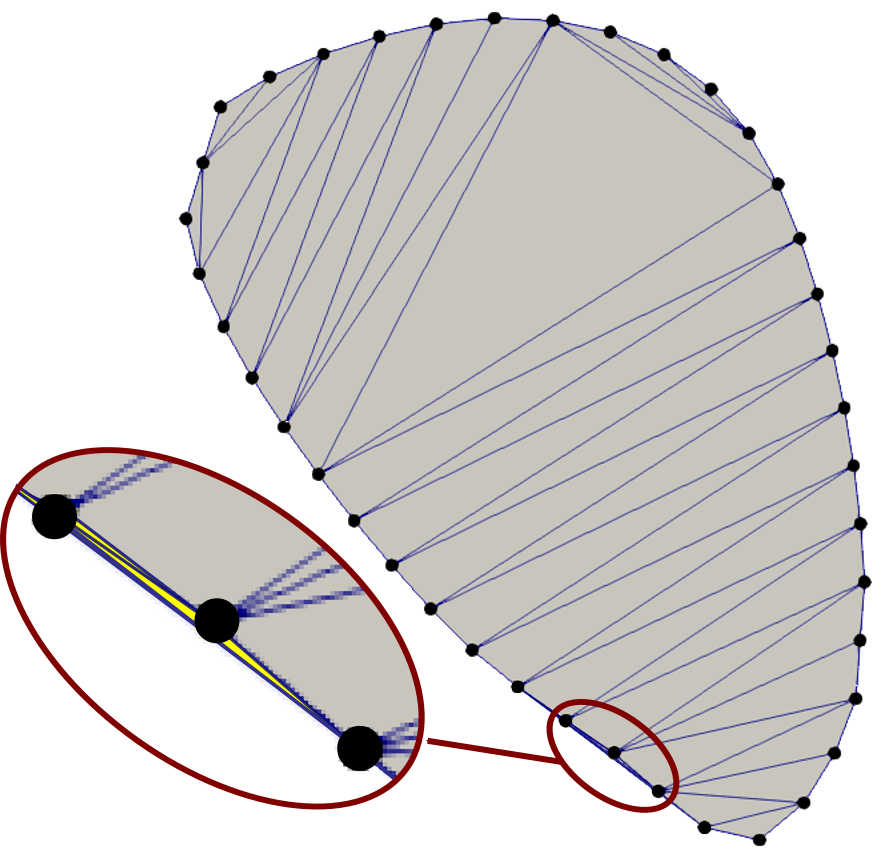
\includegraphics[width=\textwidth]{images/fiber_creation/triangulation_0.png}%
    \caption{First triangulation method}%
    \label{fig:triangulation_0}%
  \end{subfigure}
  \quad
  \begin{subfigure}[t]{0.31\textwidth}%
    \centering%
    \includegraphics[width=\textwidth]{images/fiber_creation/triangulation_1.png}%
    \caption{Second trian\-gulation method}%
    \label{fig:triangulation_1}%
  \end{subfigure}
  \quad
  \begin{subfigure}[t]{0.31\textwidth}%
    \centering%
    \includegraphics[width=\textwidth]{images/fiber_creation/triangulation_2.png}%
    \caption{Third triangulation method}%
    \label{fig:triangulation_2}%
  \end{subfigure}
  \caption{Result of different triangulation methods for a slice in the center of the biceps muscle.}%
  \label{fig:triangulations}%
\end{figure}%

\subsection{Harmonic Maps}

Next, harmonic maps are created that allow to smoothly map a given 2D reference mesh onto an actual cross-section of the muscle. The initial application of harmonic maps to meshes used for biomedical simulations is given by \cite{marchandise2010quality} and \cite{Marchandise2_2011}. The authors improve a given, oversampled surface mesh obtained from classical segmentation. This is done by partitioning the surface into multiple mesh partitions of zero genus (i.e., containing no holes) and transforming them to a reference space using harmonic maps. There, controlled remeshing is carried out before the transformation is reversed.

In our algorithm, harmonic maps are also used for the purpose of generating high quality meshes. In contrast to the literature, the mapping is based on the muscle slices instead of the surface. Also, different parameter domains are investigated.

In the algorithm, the next step is line \algref{alg:serial_algorithm_1}{alg:1.3}, to compute the harmonic maps $u$ and $v$. For a given slice $S_M$, the functions $u$ and $v$ map from points $\bfx \in S_M$ to coordinates $u(\bfx),v(\bfx)\in \R$ of a parameter domain $\Omega_P \subset \R^2$. The parameter domain is either a unit circle or a unit square.

The vector $\bfy(\bfx) := (u(\bfx), v(\bfx))^\top$ for $\bfx \in S_M$ is interpreted as position in $\Omega_P$. The maps are constructed such that the border $∂S_M$ of the slice $S_M$ is evenly mapped to the border $∂\Omega_P$ of the parameter domain $\Omega_P$.
The mapping $\bfy: S_M \to \Omega_P$ is bijective and harmonic, i.e. the Laplacians of $u$ and $v$ are zero.

More specifically, the definition is
%
\begin{equation}\label{eq:def_harmonic_maps}
  \begin{array}{l}
    u : S_M \to \R, \quad v : S_M \to \R,\\[4mm]
    Δu(\bfy) = 0, \quad Δv(\bfy) = 0 \quad \forall \bfy \in S_M.
  \end{array}
\end{equation}
%
For a uniform parametrization $\bfp:[0,1] \to ∂S_M$ of the border $∂S_M$ of the slice, i.e., 
%
\begin{align*}
  \p{l(t)}{t} = c \in \R \quad \forall t \in [0,1], \quad \text{where } l(t) := \i{0}{t} |\bfp'(\tau)| \,\d\tau,
\end{align*}
%
we require the image of the border parametrization in $\Omega_P$ to be also uniform, i.e.,%
\begin{align*}
  \p{l_P(t)}{t} = c_P \in \R \quad \forall t \in [0,1], \quad \text{where } l_P(t) := \i{0}{t} |\bfy'\big(\bfp(\tau\big)| \,\d\tau.
\end{align*}
%
Corresponding border points $\bfx_\text{M,border} \in S_M$ and $\bfx_\text{P,border} = (u_\text{P,border},v_\text{P,border})^\top$ can be defined. This leads to the following Dirichlet boundary conditions that close the definition in \cref{eq:def_harmonic_maps}:%
\begin{align}\label{eq:bc_harmonic_maps}
  u(\bfx_\text{M,border}) = u_\text{P,border}, \quad v(\bfx_\text{M,border}) = v_\text{P,border}.
\end{align}
%

\Cref{eq:def_harmonic_maps,eq:bc_harmonic_maps} describe a boundary value problem of ordinary differential equations in $u$ and $v$. We solve it using the Finite Element Method and the spatial discretization given by the triangulation of the slices.
Depending on the method of triangulation, a different number of degrees of freedom is given. For the first method with the Quickhull algorithm, no degree of freedom is present and no system of equation needs to be solved. For the third method, only one degree of freedom for the center point needs to be computed. The second method has as many degrees of freedom as there are additional points inserted during the Delaunay refinement.

The first step is to compute the prescribed border points $\bfx_\text{P,border}$ in parameter space. When using the first and third triangulation methods, the border points on the slices are  equidistant and therefore the same number of points need to be sampled equidistantly on the border $∂\Omega_P$ of the parameter space.
If the second triangulation method which potentially adds additional points is used, the same number of points  are created on the border $∂\Omega_P$ of the slice as are given on the slice $∂S_M$. The border points are created such that the relations of their distances is the same on $∂\Omega_P$ as for the original points on $∂S_M$.

Using the standard procedure of the Finite Element method for $Δu(\bfx) = 0$ on $S_M$ and $u=f(\bfx)$ on $∂S_M$, e.g. as outlined in \cite{Remacle2010}, leads to the weak form with ansatz and test functions $\phi$,
\begin{align}\label{eq:est_fe_w}
    \i{S_M}{} (\nabla u^\top \nabla \phi + \nabla f(\bfx)^\top \nabla \phi) \,\d \bfx = 0 \quad \forall \phi \in \mathcal{H}_0^1.
\end{align}
Standard linear hat functions are used on the triangles, such that they provide the interpolation property $\phi_i(\bfx_j) = \delta_{ij}$. Using the barycentric parametrization of triangles with points $\bfp^1,\bfp^2$ and $\bfp^3$ introduced in \cref{eq:barycentric_triangle}, we define the ansatz functions and get their derivatives within the elements by:
%
\begin{align*}
  \phi^{(e)}_1 &= (1 - \xi_1)(1 - \xi_2), \quad&
  \phi^{(e)}_2 &= \xi_1 (1 - \xi_2), \quad &
  \phi^{(e)}_3 &= (1 - \xi_1) \xi_2,\\[4mm]
  \nabla \phi^{(e)}_1 &= (\xi_2-1, \xi_1 - 1)^\top, \quad&
  \nabla \phi^{(e)}_2 &= (1-\xi_2, -\xi_1)^\top, \quad&
  \nabla \phi^{(e)}_3 &= (-\xi_2, 1-\xi_1)^\top.
\end{align*}
The superscript $\square^{(e)}$ refers to the definition of the functions within elements. The global assembly involves composing the global nodal functions $\phi_i(\bfx)$ for nodes indexed by $i=1, \dots, n_\text{nodes}$ and using a mapping between the barycentric coordinates $\xi_1,\xi_2 \in [0,1]^2$ inside the elements to the global coordinates $\bfx \in S_M$.
Inserting the discretization
\begin{align*}
  u_h(\bfx) = \s{i=1}{n_\text{nodes}} u_i\,\phi_i(\xi_1(\bfx), \xi_2(\bfx))
\end{align*}
into \cref{eq:est_fe_w} leads to the form
\begin{equation}\label{eq:est_weak_form}
  \begin{array}{lll}
    \s{i=1}{n_\text{nodes}}u_i \i{S_M}{} \nabla_\bfx \phi_i^\top \nabla_\bfx \phi_j \,\d\bfx + \s{i=1}{n_\text{nodes}} f_i \i{S_M}{} \nabla_\bfx \phi_i^\top \nabla_\bfx \phi_j \,\d \bfx = 0\,\quad \forall j=1,\dots,n_\text{nodes}.
  \end{array}
\end{equation}
The integrations are executed element-wise and over the elemental coordinates $\xi_1,\xi_2$. 
The transformation to elemental coordinates involves the computation of the Jacobian $J=\d\bfx/\d\bfxi$ of the mapping between element coordinates $\bfxi = (ξ_1,ξ_2)$ and global coordinates $\bfx$. From the definition in \cref{eq:barycentric_triangle} it follows that
\begin{align*}
  J = \d{\bfx}{\bfxi} = [\bfp^2-\bfp^1, \bfp^3-\bfp^1].\\[4mm]
\end{align*}
The metric tensor for this mapping is given by
\begin{align*}
  \mathcal{M} := \left(\d{x}{\bfxi}\right)^T \left(\d{x}{\bfxi}\right).
\end{align*}
%
The transformation of the integrals in \cref{eq:est_weak_form} introduces an additional integration factor of $\sqrt{\det{\mathcal{M}}}$.

We get the following matrix equation:
\begin{align}\label{eq:est_fe_system}
  M_u \bfu = -M_f\,\bff,
\end{align}
with the vector $\bfu$ of nodal solution values, the vector $\bff$ of nodal Dirichlet boundary condition values at the border and the global stiffness matrices $M_u$ and $M_f$. The two global stiffness matrices are assembled from the element stiffness matrices $M^\text{(e)}$ for the degrees of freedom at all nodes respectively at the border nodes. The entries of the element stiffness matrices are given by
\begin{align*}
  M^\text{(e)}_{i,j} = \i{0}{1}\i{0}{1-\xi_1}   \nabla \phi_i^{(e)}(\xi_1,\xi_2)^\top \, \mathcal{M}^{-1} \, \nabla \phi_j^{(e)}(\xi_1,\xi_2) \, \sqrt{\det{\mathcal{M}}}  \,\d\xi_2\d\xi_1.
\end{align*}

By solving \cref{eq:est_fe_system} for $\bfu$ we get the discretized harmonic map $u$.
The Finite Element formulation and computation for $v$ is analogous and uses the same global stiffness matrices.

\Cref{fig:harmonic_map_solution} visualizes the triangulation of $S_M$ and the solutions $u(\bfx)$ and $v(\bfx)$ in the first two plots. The color range from bright yellow to dark violet corresponds to increasing values of $u$ and $v$. It can be seen that the $u$ values increase from left to right whereas the $v$ values increase from bottom to top, corresponding to the horizontal and vertical coordinate axes $y_1$ and $y_2$ of $\Omega_P$.


Applying the computed harmonic map $\bfy(\bfx)$ to the triangulation of the slices results in a triangulation of the parameter domain $\Omega_P$. This is shown in the third plot of \cref{fig:harmonic_map_solution} and in \cref{fig:serial_alg_3}.
In both figures, the triangulation of the slices was generated using the second triangulation method with the constrained Delaunay triangulation. On the right of \cref{fig:serial_alg_3}, the image $\bfy(\bfx)$ under the harmonic map of the triangulation in the slices is shown on the unit circle parameter domains.

\begin{figure}%
  \centering%
  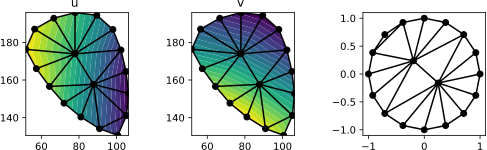
\includegraphics[width=\textwidth]{images/fiber_creation/harmonic_map_9b.pdf}%
  \caption{Triangulations and harmonic map for a slice $S_M$ of the biceps muscle. The first two plots show the solutions of $u$ and $v$ on the slice $S_M$. The third plot shows the image in $\Omega_P$ of the triangulation in $S_M$ under the harmonic map.}%
  \label{fig:harmonic_map_solution}%
\end{figure}%

\subsection{Construction of a Regular Grid in the Parameter Domain}
The next step in the \cref{alg:serial_algorithm_1} is the construction of a 2D structured, regular grid in the parameter domain $\Omega_P$, as stated in line \algref{alg:serial_algorithm_1}{alg:1.4}. This grid will then be mapped to the slices $S_M$. Creating a structured grid in a given domain is also called \emph{quadrangulation}.

The parameter domain $\Omega_P$ can be selected to be either a unit square or a unit circle. For both choices, two different schemes how to generate a grid with given number of cells can be selected.
\Cref{fig:quads} shows all four possiblities.

The first scheme, \cref{fig:quad_1}, uses an equidistant regular grid in a unit square. This is the easiest possibility to generate a quadrangulated reference domain. A possible issue concerns the corners of the square. The grid will be mapped to a cross section of the muscle which has no sharp corners. Therefore, the cells of the grid will be distorted at the corners, usually shortening diagonals that point towards the corners and lengthening the other diagonals. This assumption motivates the second scheme in \cref{fig:quad_2}. Here, the elements are already distorted in the described manner, with increasing distortion closer to the corners. The rationale is that the mapped cells in $S_M$ will then be less distorted.

A different approach is to use a unit circle, which has no corners and therefore might more resemble a muscle cross section. The first scheme of the unit circle is given in \cref{fig:quad_0}. It uses the radial and circumferential directions for the two dimensions of the grid. A disadvantage of this scheme is that the quadrilaterals at the center are degenerated to triangles. Additionally, the area of the cells varies significantly and the outer cells have unequal side lengths. To remedy this problem, the second scheme given in \cref{fig:quad_3} is constructed. When traversing from the outer border towards the center point and considering the circumferential lines of grid points, the circle morphs into a square as the number of grid points decreases. This approach has the disadvantage that some cells have an inner angle of nearly \SI{180}{\degree}, especially four elements at the border. Apart from that, all elements have similar sized sides and angles.

Each construction schemes allows to specify the (squared) number of nodes and in consequence the number of cells. The examples in \cref{fig:quad_1,fig:quad_2,fig:quad_3} have $11 \times 11$ nodes and $10 \times 10$ cells. For \cref{fig:quad_0}, the numbers are slightly different. There are $10 \times (11 + 1)$ nodes resulting in $10 \times 11$ cells.

\begin{figure}%
  \centering%
  \begin{subfigure}[t]{0.48\textwidth}%
    \centering%
    \includegraphics[width=\textwidth]{images/fiber_creation/quad_1.png}%
    \caption{Unit square, scheme 1}%
    \label{fig:quad_1}%
  \end{subfigure}
  \quad
  \begin{subfigure}[t]{0.48\textwidth}%
    \centering%
    \includegraphics[width=\textwidth]{images/fiber_creation/quad_2.png}%
    \caption{Unit square, scheme 2}%
    \label{fig:quad_2}%
  \end{subfigure}
  \begin{subfigure}[t]{0.48\textwidth}%
    \centering%
    \includegraphics[width=\textwidth]{images/fiber_creation/quad_0.png}%
    \caption{Unit circle, scheme 1}%
    \label{fig:quad_0}%
  \end{subfigure}
  \quad
  \begin{subfigure}[t]{0.48\textwidth}%
    \centering%
    \includegraphics[width=\textwidth]{images/fiber_creation/quad_3.png}%
    \caption{Unit circle, scheme 2}%
    \label{fig:quad_3}%
  \end{subfigure}
  \caption{Different quadrangulation schemes of the parameter domain with $11\times 11$ nodes. The borders of the grid are colored for better perceptiblity.}%
  \label{fig:quads}%
\end{figure}%

Next, the grid in the parameter domain is transferred to the muscle domain by applying the harmonic map $\bfy(\bfx) \in S_M$ on every point of the quadrangulation $\bfx \in \Omega_P$. This is illustrated in \cref{fig:serial_alg_4} for a parameter domain consisting of the unit circle, with quadrangulation scheme 2 and $5 \times 5$ nodes. The cells of the grid in $\Omega_P$ are shown in the right-most stack of domains. The grid points are visualized left of the grids. The resulting image of the mesh in the slices $S_M$ is shown on the left. For visualization reasons, each quadrilateral has been split into two triangles.

\subsection{Formation of Three-Dimensional Elements}

The result of the previous steps is a number of quadrangulated muscle slices. The grid on every slice has the same number of nodes and elements. The nodes on the border of neighbouring slices are positioned similarly.

The final step of \cref{alg:serial_algorithm_1} is line \algref{alg:serial_algorithm_1}{alg:1.5}, the formation of 3D elements. Inserting vertical edges between all corresponding nodes on two neighbouring slices creates a set of 3D elements and, thus, an overall 3D quadrilateral mesh of the muscle volume. This step is visualized in \cref{fig:serial_alg_8}.

\subsection{Generation of Fiber Meshes}\label{sec:generation_of_fiber_meshes}

1D fiber meshes are created following the approach of computing a divergence free vector field introduced in \cite{Choi2013}. The steps are given in \cref{alg:serial_algorithm_2}.

The Laplace problem to be solved can be stated as%
\begin{align}\label{eq:fiberest_laplace}
  Δp(\bfx) = 0 \quad \text{for } \bfx \in \Omega_M.
\end{align}
As proposed by \cite{Choi2013}, Neumann boundary conditions can be specified for the bottom and top surfaces of the muscle volume, $∂\Omega_{M, \text{bottom}}$ and $∂\Omega_{M, \text{top}}$:
\begin{equation}\label{eq:fiberest_neumann}
\begin{array}{rlrlr}
  \d{p(\bfx)}{\bfx} \cdot \bfn &= F_\text{in}, \quad &&\text{for } \bfx \in ∂\Omega_{M, \text{bottom}},\\[4mm]
  \d{p(\bfx)}{\bfx} \cdot \bfn &= F_\text{out}, \quad &&\text{for } \bfx \in ∂\Omega_{M, \text{top}}.
\end{array}
\end{equation}
The in and outflow values $F_\text{in}<0$ and $F_\text{out}>0$ are balanced such that the total inflow ${F_\text{in}\cdot \mu(∂\Omega_{M, \text{bottom}})}$ compensates the total outflow ${F_\text{in}\cdot \mu(∂\Omega_{M, \text{bottom}})}$. Here, $\mu(∂\Omega)$ is the surface area of the respective boundary.

Alternatively, Dirichlet boundary conditions can be specified:
\begin{equation}\label{eq:fiberest_dirichlet}
\begin{array}{rlrlr}
  p(\bfx) &= 0, \quad &&\text{for } \bfx \in ∂\Omega_{M, \text{bottom}},\\[4mm]
  p(\bfx) &= 1, \quad &&\text{for } \bfx \in ∂\Omega_{M, \text{top}}.
\end{array}
\end{equation}
The specification of Dirichlet boundary conditions is easier. Like Neumann boundary conditions, they enforce in and outflows orthogonal to the border.

The boundary value problem given by \cref{eq:fiberest_laplace,eq:fiberest_neumann}  or \cref{eq:fiberest_laplace,eq:fiberest_dirichlet} is discretized by the Finite Element method with linear or quadratic ansatz functions and solved by \opendihu{} using the 3D mesh generated from \cref{alg:serial_algorithm_1}. The divergence free gradient field is visualized in \cref{fig:potential_flow}. The gradient values are directly given by the Finite Element discretization. The gradient is elementwise constant for linear ansatz functions and trilinear for quadratic ansatz functions.

The next step is line \algref{alg:serial_algorithm_2}{line:2.3} in the algorithm, to trace streamline through the gradient field. Seed points are selected at the vertical center of the muscle domain and horizontally at regular subdivisions of the existing 3D elements. Because the 3D mesh was created using harmonic maps, the spacing between the seed points is very uniform.

For the tracing of streamlines, the semi-analytical Pollock's method \cite{Pollock1988} is often used, which was originally developed for fixed 2D finite difference grids. Extensions to irregular 3D grids and for given velocities at nodes instead of fluxes over faces have been formulated \cite{HAEGLAND2007Streamline}. Other, more accurate algorithms exist \cite{cordes1992continuous}, including higher order formulations \cite{juanes2006unified}.

Because modeling muscle fascicles is only a heuristic approach, the generated streamlines do not have to be exceptionally accurate. Therefore, we use a fully numeric method. The streamlines are generated by explicit Euler integration of the gradient vectors in top and bottom direction. A small spatial step width of $h=\num{1e-2}$ is used. Details of the algorithm are given in the next section, \cref{sec:algorithm_for_streamline_tracing}. In line \algref{alg:serial_algorithm_2}{line:2.4}, all generated streamlines are resampled to obtain the desired widths of the 1D elements.
\Cref{fig:fiber_tracing_streamlines} visualizes the resulting streamlines in the biceps muscle.

\begin{algorithm}
  \begin{algorithmic}[1]%
    \Statex\Procedure{Create\_1D\_meshes}{}
    \Require Structured 3D volume mesh
    \Ensure 1D fiber meshes
    \Statex
    \State Solve Laplacian flow problem   \label{line:2.2}
    \State Trace streamlines in the gradient field  \label{line:2.3}
    \State Resample 1D fiber meshes \label{line:2.4}
    \EndProcedure
  \end{algorithmic}%
  \caption{Serial algorithm}%
  \label{alg:serial_algorithm_2}%
\end{algorithm}%

\begin{figure}%
  \centering%
  \begin{subfigure}[t]{0.48\textwidth}%
    \centering%
    \includegraphics[height=10cm]{images/fiber_creation/potential_flow.png}%
    \caption{Solution (color coding) and direction vectors of the gradient field for the boundary value problem \cref{eq:fiberest_laplace} with Dirichlet boundary conditions \cref{eq:fiberest_dirichlet}.}%
    \label{fig:potential_flow}%
  \end{subfigure}
  \quad
  \begin{subfigure}[t]{0.48\textwidth}%
    \centering%
    \includegraphics[height=10cm]{images/fiber_creation/streamlines_red.png}%
    \caption{Resulting streamlines that were traced through the gradient field.}%
    \label{fig:fiber_tracing_streamlines}%
  \end{subfigure}
  \caption{Setup and solution of the Laplace problem for the biceps geometry that is used to estimate muscle fibers by streamline tracing.}%
  \label{fig:potential_flow_streamlines}%
\end{figure}%

\subsection{Algorithm for Streamline Tracing}\label{sec:algorithm_for_streamline_tracing}
The algorithm for streamline tracing uses an efficient method to traverse the mesh, which makes use of its structuredness.
At first, the element $E^{(0)}$ in the mesh that contains the first seed point $\bfp^0$ needs to be found. By construction of the mesh generation algorithms, this is always the element with the lowest index. 
However, if the seed points is not found there, the scheme is robust enough to search in all other elements.

Starting from the seed point $\bfp^0 = \bfp^{(i)}$ in element $E^{(i)}$, the next point $\bfp^{(i+1)}$ of a streamline is computed as %
\begin{align*}
  \bfp^{(i+1)} = \bfp^{(i)} + h\,\nabla p (\bfp^{(i)}).
\end{align*}
After $\bfp^{(i+1)}$ has been computed, the mesh element $E^{(i+1)}$ where it is located needs to be identified. It is needed to evaluate the gradient value $\nabla p (\bfp^{(i+1)})$ at the new point. 

At first, the element $E^{(i)}$ of $\bfp^{(i)}$ is checked whether it also contains $\bfp^{(i+1)}$. If not, the neighboring element in the direction of the streamline is considered. This neighboring element is chosen among all up to 26 possible neighbors such that the direction from the previous element $E^{(i-1)}$ to the current element $E^{(i)}$ continues.

If this element is also not the right one, all other neighbors of $E^{(i)}$ are subsequently checked, ordered by their plausibility according to the previous streamline direction. If none of the 27 considered elements contains the computed point, a search among all elements of the entire mesh is performed. This case happens only for unsuited choices of the integration width $h$, i.e., if the streamline tracing skips whole elements.

The end of a streamline is detected when the streamline reaches the final $z$ plane, either at the bottom or top of the muscle volume. To make the algorithm more robust, also the case is considered where the streamline leaves the muscle domain to the side shortly before reaching the end of the muscle. This can happen due to discretization errors for streamlines that start close to the border of the muscle. In such a case, the missing rest of the streamline is interpolated from up to four existing neighboring parallel streamlines.

After the end of the streamline is found, tracing of the next streamline starts at the next seed point $\bfp^0_\text{next}$. For this purpose, the element where $\bfp^0_\text{next}$ is located is required next. At first, this element is searched among all elements with the same $z$ coordinates as the previous seed point. The strategy for this search in a 2D grid of elements is analogous to the previously explained search in the 3D grid of elements for the streamlines: First, the element of the previous seed point is checked. Then, the most plausible neighbor, the one opposite to the previous element, is checked. With this scheme, new seed points are predicted along the $x$ axis of the 3D mesh.

After a row of elements with seed points in $x$ direction is completed, the next row of elements begins parallel to the previous one. Accordingly, the algorithm knows to switch to the new row after the end in $x$ direction was reached.

The presented scheme avoids traversing all elements of the mesh by predicting the next elements according to streamline direction and organization of seed points. This is facilitated by the structured mesh, which has well-defined element neighbor relations.
At the same time, the scheme is robust enough to also efficiently handle streamlines in other use cases. It can also be reused, e.g., for non-vertex free vector fields or in muscle fiber tracing applications of more complex shaped muscle where the fibers change directions.

\subsection{Results and Discussion}\label{sec:mesh_generation_0_results_and_discussion}
The presented \cref{alg:serial_algorithm_1,alg:serial_algorithm_2} generate a 3D mesh and 1D muscle fibers from a triangulated surface. Three different triangulation strategies for the slices and four different reference quadrangulations can be chosen. In the following, the different choices are evaluated.

The different triangulation methods for the slices that are discussed in \cref{sec:triangulation_of_the_slices} are visualized in the three columns of \cref{fig:tri_triangulations}. 
The top rows show the triangulation of $S_M$ and the harmonic map $u$ as color coded value from violet to yellow. $u$ is the horizontal coordinate on the reference domain. A point with violet color in $S_M$ will be mapped to a left-most point in the parameter space $\Omega_P$. Similarly, a yellow point will be mapped to a point far at the right in $\Omega_P$.

The middle and bottom rows in \cref{fig:tri_triangulations} show the image of the triangulation in $\Omega_P$ under the harmonic map, for the unit square and the unit circle, respectively. The mapping between the colored border points stems from the Dirichlet boundary conditions in the formulation of the harmonic map. In consequence, the border points are by construction equally spaced both in the muscle domain $S_M$ and in the parameter domain $\Omega_P$.

It can be seen that the triangulation appears distorted in the parameter domains. The effect is highest for the square in the columns \cref{fig:triu_1} and \cref{fig:triu_2}. For the latter the center point of the muscle domain $S_M$ gets mapped far off the center of the squared parameter domain. This effect does not occur for the circle.

The reason for this lies in the triangulation of $S_M$ together with the border shape. In the third method, only the value at the center point is a degree of freedom in the computation of $u$ while the values at the border points are fixed. By the triangulation, the value of $u$ varies linearly from the border towards the center point.
By comparing the colored border points in the muscle slice in the top row with the square in the second row, it can be seen that the prescribed values for $u$ are 0 at all blue points, 1 at all yellow points and linearly increasing from 0 to 1 at the green and red points, increasing from left to right.
The yellow points of $S_M$ with the prescribed constant value of $u=1$ are approximately located on a vertical line. The first two derivatives of $u$ in vertical coordinate direction are therefore almost zero, in consequence, the Laplace equation forces the derivatives in horizontal direction to also be approximately zero. Therefore, the solution value at the center point becomes close to $1$. This leads to the mapped center point being close to the right border in the square parameter domain. The same happens for the vertical coordinate $v$ of the harmonic map.

For the circle, neighboring border points are not located on horizontal or vertical lines and, thus, the Dirichlet bondary conditions for $u$ and $v$ vary along the border. Therefore, a better mapping is obtained. The shape of the muscular slice is more similar to the circle than to the square.

Another result that can be seen in \cref{fig:tri_triangulations} is the effect on the harmonic map of the failure of the first method to handle concave slices. As the top left image shows, the first triangulation method produces triangles outside the domain. The triangles are located around the red border points. In the square parameter domain, these triangles are degenerated and lie on the bottom border. In the circle parameter domain where the respective triangles can be seen at the bottom they even intersect other triangles. This yields an invalid triangulation.

The reasons for degenerate triangles in the square parameter domains are not solely the concave muscle slices. Also, the straight sides of the unit square lead to degenerate triangles whenever three border points of the same side form a triangle.
In the example in \cref{fig:tri_triangulations} this occurs for the square in column (\subref{fig:triu_0}). As can be seen in the triangulated slice in the top row, there are three triangles that are entirely made up of blue border points. These triangles get mapped onto the left side of the square parameter domain where they have a vanishing surface area.

The same effect also occurs with the second triangulation method in column (\subref{fig:triu_1}) where a triangle at the bottom right is comprised of three red border points and therefore gets mapped to the bottom side of the square. Because of the guaranteed minimum angle in the second triangulation method this circumstance occurs less often and only for muscle cross-sections where the border makes sharp turns, such as the muscle slice in this example. The third triangulation method is guaranteed to avoid this problem as all triangles are connected with the center point.

% ------------------
% parameter space triangulations
\begin{figure}%
  \centering%
  \begin{subfigure}[t]{0.31\textwidth}%
    \centering%
    \includegraphics[width=\textwidth]{images/fiber_creation/u_0.png}%
    \caption{First method,\\Quickhull agorithm}%
    \label{fig:triu_0}%
  \end{subfigure}
  \quad
  \begin{subfigure}[t]{0.31\textwidth}%
    \centering%
    \includegraphics[width=\textwidth]{images/fiber_creation/u_1.png}%
    \caption{Second method,\\Delaunay refinement}%
    \label{fig:triu_1}%
  \end{subfigure}
  \quad
  \begin{subfigure}[t]{0.31\textwidth}%
    \centering%
    \includegraphics[width=\textwidth]{images/fiber_creation/u_2.png}%
    \caption{Third method,\\center of gravity}%
    \label{fig:triu_2}%
  \end{subfigure}\\
  
  % square
  \begin{subfigure}[t]{0.31\textwidth}%
    \centering%
    \includegraphics[width=0.9\textwidth, trim=37mm 14mm 6mm 6mm, clip]{images/fiber_creation/mesh_plots/out_0_1_0_tri.png}%
    %\caption{}%
    \label{fig:w_01}%
  \end{subfigure}
  \quad
  \begin{subfigure}[t]{0.31\textwidth}%
    \centering%
    \includegraphics[width=0.9\textwidth, trim=37mm 14mm 6mm 6mm, clip]{images/fiber_creation/mesh_plots/out_1_1_0_tri.png}%
    %\caption{}%
    \label{fig:w_11}%
  \end{subfigure}
  \quad
  \begin{subfigure}[t]{0.31\textwidth}%
    \centering%
    \includegraphics[width=0.9\textwidth, trim=37mm 14mm 6mm 6mm, clip]{images/fiber_creation/mesh_plots/out_2_1_0_tri.png}%
    %\caption{}%
    \label{fig:w_21}%
  \end{subfigure}\\
  
  % circle
  \hspace{-12mm}
  \begin{subfigure}[t]{0.31\textwidth}%
    \centering%
    \includegraphics[width=0.9\textwidth, trim=37mm 14mm 6mm 6mm, clip, angle=225,origin=c]{images/fiber_creation/mesh_plots/out_0_0_0_tri.png}% trim=left bottom right top, clip]
    %\caption{}%
    \label{fig:w_00}%
  \end{subfigure}
  \quad
  \begin{subfigure}[t]{0.31\textwidth}%
    \centering%
    \includegraphics[width=0.9\textwidth, trim=37mm 14mm 6mm 6mm, clip, angle=225,origin=c]{images/fiber_creation/mesh_plots/out_1_0_0_tri.png}%
    %\caption{}%
    \label{fig:w_10}%
  \end{subfigure}
  \quad
  \begin{subfigure}[t]{0.31\textwidth}%
    \centering%
    \includegraphics[width=0.9\textwidth, trim=37mm 14mm 6mm 6mm, clip, angle=225,origin=c]{images/fiber_creation/mesh_plots/out_2_0_0_tri.png}%
    %\caption{}%
    \label{fig:w_20}%
  \end{subfigure}
  
  \caption{Top row: Different triangulation methods for $S_M$, the color represents the solution $u$ of the harmonic map. Middle and bottom row: triangulation mapped to the parameter domain $\Omega_P$, for the unit square (middle) and the unit circle (bottom). Each column corresponds to one triangulation method.}%
  \label{fig:tri_triangulations}%
\end{figure}%



In the next step, the algorithm creates a quadrilateral mesh in the parameter domain and computes its image in the muscle domain using the inverse of the harmonic map. The results are shown in \cref{fig:tri_meshes} for the three different triangulation methods (columns) and the four different schemes to create the quadrilateral mesh (rows).

In the images in column (\subref{fig:tu_2}) and rows (\subref{fig:tquad_1}) and (\subref{fig:tquad_2}) it can be seen that the previously observed effect of a bad mapping for squares and the third triangulation method also leads to a mesh in $S_M$ of poor quality.
The result for the two square schemes in column (\subref{fig:tu_1}) is better but still not satisfactory. Good results with the square reference domain are only observed for the first triangulation method in this example.

It can be seen that the approximation quality of the border of the domain varies. Most of all, the combination of the first triangulation method (column (\subref{fig:tu_0})) and the square parameter domain (rows (\subref{fig:tquad_1}) and (\subref{fig:tquad_2})) reproduces the shape of the slice poorly. 
The mismatch occurs at the blue and red border points. Additionally, the second triangulation method (column (\subref{fig:tu_1})) for the squares fails to correctly represent the round border at the bottom of the domain.
The degenerate triangles in the parameter domain are the cause for this effect. The harmonic map $\bfy: S_M \to \Omega_P$ is not injective and therefore its inverse does not exist. In our implementation, the points on the degenerate triangles in $\Omega_P$ are mapped anywhere inside the corresponding triangles in $S_M$. Thus, the mapping is correctly inverted at locations of valid triangles and only creates different border points in the invalid areas.


Furthermore, it can be seen that an inaccurate representation of the border also occurs with the parameter mesh in the unit circle generated by scheme 1. In this case, the reason is the low number of elements at the border in the parameter domain quadrangulation.

The two schemes for the circle parameter domain in rows (\subref{fig:tquad_0}) and (\subref{fig:lquad_3}) both generate reasonable meshes for all triangulation methods, despite the different structure of the generated meshes. The best results for both schemes occur with the third triangulation method.

% ------------------
% resulting meshes
\begin{figure}%
  \centering%
  \hspace{0.24\textwidth}
  \begin{subfigure}[t]{0.24\textwidth}%
    \centering%
    \includegraphics[width=\textwidth]{images/fiber_creation/u_0.png}%
    \caption{First method}%
    \label{fig:tu_0}%
  \end{subfigure}
  \begin{subfigure}[t]{0.24\textwidth}%
    \centering%
    \includegraphics[width=\textwidth]{images/fiber_creation/u_1.png}%
    \caption{Second method}%
    \label{fig:tu_1}%
  \end{subfigure}
  \begin{subfigure}[t]{0.24\textwidth}%
    \centering%
    \includegraphics[width=\textwidth]{images/fiber_creation/u_2.png}%
    \caption{Third method}%
    \label{fig:tu_2}%
  \end{subfigure}\\
  
  % square
  \begin{subfigure}[t]{0.24\textwidth}%
    \centering%
    \includegraphics[width=\textwidth]{images/fiber_creation/quad_1.png}%
    \caption{Square, scheme 1}%
    \label{fig:tquad_1}%
  \end{subfigure}
  \begin{subfigure}[t]{0.24\textwidth}%
    \centering%
    \includegraphics[width=\textwidth, trim=26mm 14mm 6mm 6mm, clip]{images/fiber_creation/mesh_plots/out_0_1_0_w.png}%
    %\caption{}%
    \label{fig:tri_01}%
  \end{subfigure}
  \begin{subfigure}[t]{0.24\textwidth}%
    \centering%
    \includegraphics[width=\textwidth, trim=30mm 14mm 6mm 6mm, clip]{images/fiber_creation/mesh_plots/out_1_1_0_w.png}%
    %\caption{}%
    \label{fig:tri_11}%
  \end{subfigure}
  \begin{subfigure}[t]{0.24\textwidth}%
    \centering%
    \includegraphics[width=\textwidth, trim=30mm 14mm 6mm 6mm, clip]{images/fiber_creation/mesh_plots/out_2_1_0_w.png}%
    %\caption{}%
    \label{fig:tri_21}%
  \end{subfigure}\\[-4mm]
  
  % square adjusted
  \begin{subfigure}[t]{0.24\textwidth}%
    \centering%
    \includegraphics[width=\textwidth]{images/fiber_creation/quad_2.png}%
    \caption{Square, scheme 2}%
    \label{fig:tquad_2}%
  \end{subfigure}
  \begin{subfigure}[t]{0.24\textwidth}%
    \centering%
    \includegraphics[width=\textwidth, trim=26mm 14mm 6mm 6mm, clip]{images/fiber_creation/mesh_plots/out_0_2_0_w.png}%
    %\caption{}%
    \label{fig:tri_02}%
  \end{subfigure}
  \begin{subfigure}[t]{0.24\textwidth}%
    \centering%
    \includegraphics[width=\textwidth, trim=30mm 14mm 6mm 6mm, clip]{images/fiber_creation/mesh_plots/out_1_2_0_w.png}%
    %\caption{}%
    \label{fig:tri_12}%
  \end{subfigure}
  \begin{subfigure}[t]{0.24\textwidth}%
    \centering%
    \includegraphics[width=\textwidth, trim=30mm 14mm 6mm 6mm, clip]{images/fiber_creation/mesh_plots/out_2_2_0_w.png}%
    %\caption{}%
    \label{fig:tri_22}%
  \end{subfigure}\\[-4mm]
  
  % circle
  \begin{subfigure}[t]{0.24\textwidth}%
    \centering%
    \includegraphics[width=\textwidth]{images/fiber_creation/quad_0.png}%
    \caption{Circle, scheme 1}%
    \label{fig:tquad_0}%
  \end{subfigure}
  \begin{subfigure}[t]{0.24\textwidth}%
    \centering%
    \includegraphics[width=\textwidth, trim=26mm 14mm 6mm 6mm, clip]{images/fiber_creation/mesh_plots/out_0_0_0_w.png}% trim=left bottom right top, clip]
    %\caption{}%
    \label{fig:tri_00}%
  \end{subfigure}
  \begin{subfigure}[t]{0.24\textwidth}%
    \centering%
    \includegraphics[width=\textwidth, trim=26mm 14mm 6mm 6mm, clip]{images/fiber_creation/mesh_plots/out_1_0_0_w.png}%
    %\caption{}%
    \label{fig:tri_10}%
  \end{subfigure}
  \begin{subfigure}[t]{0.24\textwidth}%
    \centering%
    \includegraphics[width=\textwidth, trim=30mm 14mm 6mm 6mm, clip]{images/fiber_creation/mesh_plots/out_2_0_0_w.png}%
    %\caption{}%
    \label{fig:tri_20}%
  \end{subfigure}\\[-4mm]
  
  % circle adjusted
  \begin{subfigure}[t]{0.24\textwidth}%
    \centering%
    \includegraphics[width=\textwidth]{images/fiber_creation/quad_3.png}%
    \caption{Circle, scheme 2}%
    \label{fig:lquad_3}%
  \end{subfigure}
  \begin{subfigure}[t]{0.24\textwidth}%
    \centering%
    \includegraphics[width=\textwidth, trim=30mm 14mm 6mm 6mm, clip]{images/fiber_creation/mesh_plots/out_0_3_0_w.png}%
    %\caption{}%
    \label{fig:tri_03}%
  \end{subfigure}
  \begin{subfigure}[t]{0.24\textwidth}%
    \centering%
    \includegraphics[width=\textwidth, trim=30mm 14mm 6mm 6mm, clip]{images/fiber_creation/mesh_plots/out_1_3_0_w.png}%
    %\caption{}%
    \label{fig:tri_13}%
  \end{subfigure}
  \begin{subfigure}[t]{0.24\textwidth}%
    \centering%
    \includegraphics[width=\textwidth, trim=30mm 14mm 6mm 6mm, clip]{images/fiber_creation/mesh_plots/out_2_3_0_w.png}%
    %\caption{}%
    \label{fig:tri_23}%
  \end{subfigure}
  \caption{Meshes in $S_M$ for quadrangulations (rows) and triangulations (columns).}%
  \label{fig:tri_meshes}%
\end{figure}%

% quantitative quality plots of results
Next, a quantitative comparison of the resulting mesh quality for different parameters of the presented algorithm is carried out. The mesh quality could easily be improved by a smoothing step, e.g. by applying Laplacian smoothing \cite{field1988laplacianSmoothingAndDelaunayTriangulations}. This technique iteratively improves the local mesh quality. Because of the local scheme, the quality of the final result depends on the quality of the initial mesh. Therefore, the following study forgoes additional smoothing steps and evaluates the direct outcome of the meshing algorithm.

The algorithm was executed for all variants with 43 slices of the biceps muscle, resulting in 43 meshes for every combination of triangulation method and quadrangulation scheme. In each generated mesh the edge lengths of the elements were collected and normalized to have a mean of 1. 
The normalization was done to allow a comparison between meshes with different bounding box sizes.
The standard deviation of the normalized lengths was determined in each mesh. The total mean of all the standard deviations was computed. This value is a measure for the quality of the mesh. A low value means that in every slice the generated mesh has similar edge length and, in consequence, the overall mesh has good quality.

\begin{figure}%
  \centering%
  \includegraphics[width=\textwidth]{images/fiber_creation/mesh_quality.pdf}%
  \caption{Mesh quality (red, lower is better) and duration (yellow) for the three different triangulation methods and the different parameter space quadrangulation schemes. A low value for the standard deviation of relative element lengths indicates good quality.}%
  \label{fig:mesh_quality}%
\end{figure}

\Cref{fig:mesh_quality} visualizes the results. Three groups of bars are displayed for the three triangulation methods. For every type of mesh in the parameter space, i.e. unit square ($\square$) or unit circle ($\ocircle$) and scheme 1 or 2, the standard deviation is given by the red bar and the duration of the overall algorithm is given by the yellow bar. The corresponding axis labels for standard deviation and duration are given on the left and right of the diagram.

The diagram shows the lowest standard deviation of edges and therefore the best mesh quality for the first triangulation method and the square ($\square 1$ and $\square 2$), with scheme 1 having a slightly better value than scheme 2. This shows that the modified placement of the nodes in scheme 2 has no positive effect compared to scheme 1.
However, from the observations in \cref{fig:tri_triangulations} it is known that the borders are not represented correctly.
This behaviour does not influence the result because of the chosen metric of uniform relative edge lengths.
Similar good results can be seen for scheme 2 in the circular parameter domain and the second and third triangulations.

Moreover, it can be seen that certain connections between parameter domain and suited triangulation scheme exist. The square parameter domain works best with the first triangulation method. The second scheme for the parameter mesh on the unit circle works best with the triangulation methods 2 and 3.

The first scheme for the parameter mesh on the unit circle ($\ocircle 1$) shows bad results for all triangulation methods. This can be explained by looking at the generated meshes in row (\subref{fig:tquad_0}) of \cref{fig:tri_meshes}. By construction, the elements have a bad aspect ratio. This results in the high standard deviation values. However, the generated meshes still look uniform to a certain extent and can be useful in applications where such type of mesh is needed. The score could be improved by adding more nodes in circumferential direction.

The runtime of the algorithm is approximately the same for the different parameter domain meshes. It mainly depends on the triangulation of the slices. The first triangulation using the \emph{SciPy} package takes the most time, followed by the Delaunay refinement. The fastest triangulation is the custom one where only one additional point needs to be placed. In conclusion, when runtime is an issue, the third triangulation should be chosen. It achieves good quality meshes only with the second scheme of the circular parameter domain. This combination also does not suffer from the bad approximation quality of the border, as is the case for the unit circle with the first triangulation method.

\Cref{fig:tendon_meshes} shows three structured meshes $\Omega_{T,i}$ for the tendons of the biceps brachii muscle that were created using \cref{alg:serial_algorithm_1}. The tendon at the bottom of the muscle are represented by a single mesh. At the top there are two tendons that extend the two muscle heads of the biceps. Because the meshes need to be structured two tendon meshes are created at the top. It can be seen that the algorithm creates meshes with similar sized elements despite the difficult, wound geometry of the surfaces.

\begin{figure}
  \centering
  \begin{tabular}{cc}
    \begin{tabular}[b]{c}
      \begin{subfigure}[b]{0.60\textwidth}%
        \centering%
        \includegraphics[width=\textwidth]{images/fiber_creation/tendon2_.png}
        \caption{Two meshes for the top tendons with $9 \times 9 \times 21 = \num{1701}$ nodes each.}%
        \label{fig:tendon2}%
      \end{subfigure} \\
      \begin{subfigure}[b]{0.60\textwidth}%
        \centering%
        \includegraphics[width=\textwidth]{images/fiber_creation/tendon1.png}
        \caption{One mesh for the bottom tendon with $5 \times 5 \times 25 = \num{525}$ nodes.}%
        \label{fig:tendon1}%
      \end{subfigure}
    \end{tabular}
    &
    \begin{subfigure}[b]{0.30\textwidth}%
      \centering%
      \includegraphics[width=\textwidth]{images/fiber_creation/muscle_with_tendons.png}
      \caption{The tendon meshes in the volume of the whole biceps muscle.}%
      \label{fig:muscle_with_tendons}%
    \end{subfigure}
  \end{tabular}
  \caption{Tendon meshes that were created using the serial algorithm for mesh creation.}%
  \label{fig:tendon_meshes}%
\end{figure}%

\begin{reproduce}
  The described algorithms are part of the \code{fiber_tracing} examples. Execute the following commands to get the results in this chapter:
  \begin{lstlisting}[columns=fullflexible,breaklines=true,postbreak=\mbox{\textcolor{gray}{$\hookrightarrow$}\space}]
    cd $\$$OPENDIHU_HOME/examples/fiber_tracing/streamline_tracer/scripts
    . run_evaluation.sh
  \end{lstlisting}
  Then, the visualizations will be created under \code{../processed_meshes}. Create \cref{fig:mesh_quality} with \code{plot_mesh_quality.py}.
  How to create the tendon meshes is explained at the end of \cref{sec:repro_tendon_meshes}.
\end{reproduce}


%
\section{Parallel Algorithm to Create Muscle and Fiber Meshes}\label{sec:parallel_algorithm}

The previously presented algorithm to create 3D and 1D meshes is not parallelized. 
This restricts the resources that can be employed during the execution of the algorithm to those accessible by one hardware core.
Thus, the size of the handled meshes is limited by the available memory of the computer.
An algorithm that can be used with shared memory parallelization could, in contrast, benefit from more total memory that is accessible at different cores. Furthermore, the tracing of the streamlines could be performed in parallel which has the potential to reduce runtimes.

In the following, we present an extended algorithm based on the one presented in \cref{sec:ser_alg_meshes} that can be run in parallel on multiple cores. The extended algorithm employs a partitioning of the 3D volume. Every process only stores data corresponding to its own partition. This allows to run the algorithm on a shared memory system, where data transfer between the processes occurs by sending messages using the Message Passing Interface (MPI). It is possible to create meshes with larger sizes than could fit into a single processes' memory. This enables the algorithm for meshes with very high resolution that can be used for simulations in the field of High Performance Computing. 
These meshes are partitioned into subdomains for every compute core and can be read from and written to disk concurrently.

\subsection{Overview of the Parallel Algorithm to Create Muscle and Fiber Meshes}

The steps of the algorithm and its input and output are given in \cref{alg:parallel_algorithm_1}. Input and output are the same as for the \cref{alg:serial_algorithm_1} presented in \cref{sec:ser_alg_meshes}. The input is a triangulated tubular surface of the muscle that can be obtained as described in \cref{sec:preprocessing_of_the_muscle_geometry}. A second input, the variable called \emph{border\_points}, is used only during recursive calls and is not set at the beginning. The output consists of the 3D mesh of the muscle volume $\Omega_M$ and embedded 1D fiber meshes $\Omega_{F,i}$. 

During execution of the algorithm, the 3D mesh of the muscle is recreated iteratively with increasing resolution and increasing number of subdomains. The algorithm is formulated recursively. At first, a single process executes all the steps listed in lines \algref{alg:parallel_algorithm_1}{line:3.2} to \algref{alg:parallel_algorithm_1}{line:3.11a}. This corresponds to recursion level $\ell=0$. Then, in line \algref{alg:parallel_algorithm_1}{line:3.12} the procedure is called again and in the first recursion executed by eight processes with eight subdomains. On the $\ell$th recursion level, the number of involved processes and subdomains is $8^\ell$. After a specified maximum recursion depth $\ell_\text{max}$ is reached, all involved processes execute the first branch of the \code{if} statement in line \algref{alg:parallel_algorithm_1}{line:3.8} and generate the final output meshes in \algref{alg:parallel_algorithm_1}{line:3.9}.

In more detail, the goal during the recursive calls is to determine smooth borders for the subdomains. At the end of the algorithm, the constructed partitioning is used to create the final 3D mesh. On each recursion level, the subdomain borders are determined by tracing streamlines through the entire muscle volume, similar to the approach in \cref{alg:serial_algorithm_2}. For this purpose, a new 3D mesh is created on each level and a global Laplace problem is solved on the mesh. The number of elements in this mesh increases by the factor of eight on each level. All subdomain borders are determined anew on each recursion level. This means that the subdomain borders change slightly as the mesh refines.

As the subdomain borders in the interior of the volume refine, so do the outer borders given by the surface of the muscle. The given triangulation of the surface is sampled again on each recursion level yielding increasingly fine representations.

The steps in \cref{alg:parallel_algorithm_1} are executed concurrently by the involved processes at the respective level.
Some of the steps only operate on the locally stored data and, thus, are independent of other processes. Other steps involve communication between processes. Whether an instruction effects only the own domain of the process or involves global communication is denoted in parantheses at the beginning of the lines in \cref{alg:parallel_algorithm_1}.

\begin{algorithm}
  \begin{algorithmic}[1]%
    \Procedure{Create\_3D\_meshes\_parallel}{}
    \Require Triangulated tubular surface
    \Require border\_points: $4\times 4$ points per slice
    \Ensure Structured 3D volume mesh
    \Ensure 1D fiber meshes
    \Statex
    \State (own domain) Create\_3D\_mesh(border\_points)        \label{line:3.2}
    \State (own domain) Fix and smooth 2D meshes  \label{line:3.3}   
    \State (global)$\hskip2.4em$     Solve Laplace problem       \label{line:3.4}
    \State (global)$\hskip2.4em$      Communicate ghost elements to neighboring subdomains      \label{line:3.5}
    \State (own domain) Trace streamlines for new subdomain boundaries      \label{line:3.6}
    \State (global)$\hskip2.4em$      new\_border\_points $\leftarrow$ Construct new subdomains      \label{line:3.7}
    \Statex
    \If{recursion ends}         \label{line:3.8}
    \State (own domain) Trace streamlines for fiber meshes      \label{line:3.9}
    \Else      \label{line:3.10}
    \State (global)$\hskip2.4em$      communicate border points      \label{line:3.11a}
    \State (global)$\hskip2.4em$      Create\_3D\_meshes\_parallel(new\_border\_points)      \label{line:3.11}
    \EndIf      \label{line:3.12}
    \EndProcedure
  \end{algorithmic}%
  \caption{Parallel algorithm to create muscle and fiber meshes}%
  \label{alg:parallel_algorithm_1}%
\end{algorithm}%

\subsection{Generation of the 3D Mesh}
Next, the steps of the algorithm are discussed in detail.
\Cref{alg:parallel_algorithm_1} starts its execution with one process and a triangulation of the tubular muscle surface being the only input. The following procedure is described in this section with a focus on the serial execution in this first call.

The first step in line \algref{alg:parallel_algorithm_1}{line:3.2} is to execute \cref{alg:serial_algorithm_1} to generate a 3D mesh of the volume. The second triangulation method is used with a circular reference domain quandrangulated by the second scheme as explained in \cref{sec:ser_alg_meshes}.

Next, line \algref{alg:parallel_algorithm_1}{line:3.3} improves the mesh quality of the 2D muscle slices $S_M$ from which the 3D mesh is formed. This action consists of two steps. The first step is to ensure that no self-intersecting or degenerate quadrilaterals exist in the slice. The second step applies Laplacian smoothing to improve the mesh quality of the slice.

Theoretically, the first step should not be necessary, as the chosen quadrangulation algorithm always produces valid elements. However, in practice, small or irregularly shaped, concave domains occur and together with rounding and numerical errors in the Laplace problem computations lead to invalid meshes with self intersecting elements, especially for higher recursion depths in \cref{alg:parallel_algorithm_1}. Executing the first step therefore increases the robustness of the implementation.

\begin{figure}%
  \centering%
  \def\svgwidth{0.7\textwidth}%
  \input{images/parallel_fiber_estimation/quads.pdf_tex}%
  \caption{A quadrilateral (left) and the four triangles (right) that can be constructed from its four points. These triangles are needed for the check in \cref{alg:parallel_algorithm_1} if the quadrilateral is valid.}%
  \label{fig:quads_tris}%
\end{figure}%

The algorithm performs this step by repeatedly iterating over all interior mesh points in every slice $S_M$ and fixing invalid elements. To find invalid elements, for every quadrilateral the four triangles that can be formed from the points of the quadrilateral are considered, as shown in \cref{fig:quads_tris}.
For every triangle with points $\bfp^0,\bfp^1$ and $\bfp^2$, the orientation of the triangle is determined. The orientation is counterclockwise if the oriented triangle area $A_{012}$ is positive. The oriented triangle area is the determinant of the $3 \times 3$ matrix that contains the row vectors $(p^i_x,p^i_y,1)$ for the triangle points $\bfp^i=(p^i_x,p^i_y)^\top$ and can be computed by the following formula \cite{sedgewick2011algorithms}:
%
\begin{align*}
  A_{012} = (p^1_x-p^0_x)\,(p^2_y-p^0_y) - (p^2_x-p^0_x)\,(p^1_y-p^0_y).
\end{align*}
If the orientation is counterclockwise, a score value of the triangle is set to one, if it is clockwise, the score is set to zero. The score values of the four triangles are added up to yield a score $s$ for the quadrilateral. Only if this score is $s \geq 3$, the quadrilateral is considered valid. For $s = 3$ the quadrilateral is concave, for $s=4$ it is convex.

At the current mesh point in the loop over all points that are not at the border of the mesh, the four adjacent quadrilaterals are considered. If any of them is invalid, the algorithm tries to improve the situation by deflecting the point by a random, small vector. A maximum of 200 random deflections from the original position with exponentially increasing deflection vector sizes are tried. After each modification of the point the scores of the four adjacent quadrilateral elements are evaluated. If the sum of the four element scores increases, the point is kept and the iteration over all interior mesh points starts anew. 

Note that this does not necessarily mean that the invalid element was fixed, only its score was improved. If it was not fixed, it will be considered again in the next iteration. For example, a convex element that initially is oriented clockwise instead of counterclockwise has a score of $s=0$. In the first iteration, one point is deflected such that the quadrilateral intersects itself but has a higher score $s\geq 0$. At least one more iteration is needed until the quadrilateral is oriented correctly.
When all elements in the slice $S_M$ are valid, this step is complete.

The second step is the smoothing step that improves the mesh quality of the 2D slices. \num{20} iterations of Laplacian smoothing \cite{field1988laplacianSmoothingAndDelaunayTriangulations} are executed. Laplacian smoothing in our case subsequently visits all points of the mesh and sets the location of a point to the center of gravity of its eight neighbours. \Cref{fig:laplace_smoothing} shows the effect of Laplacian smoothing for a slice in a subdomain on the first recursion level. It can be seen how the smoothing equalizes the element lengths and angles.

\begin{figure}%
  \centering%
  \begin{subfigure}[t]{0.48\textwidth}%
    \centering%
    \includegraphics[height=7cm]{images/parallel_fiber_estimation/world_mesh.png}
    \caption{Initial 2D mesh of a subdomain at the border of the biceps muscle.}%
    \label{fig:world_mesh}%
  \end{subfigure}
  \quad
  \begin{subfigure}[t]{0.48\textwidth}%
    \centering%
    \includegraphics[height=7cm]{images/parallel_fiber_estimation/world_mesh_improved.png}
    \caption{The mesh of (\subref{fig:world_mesh}) after 20 iterations of Laplacian smoothing.}%
    \label{fig:world_mesh_improved}%
  \end{subfigure}    
  \caption{Effect of Laplacian smoothing of a 2D grid which occurs in line \algref{alg:parallel_algorithm_1}{line:3.3} of \cref{alg:parallel_algorithm_1}.}%
  \label{fig:laplace_smoothing}%
\end{figure}%

\subsection{Computation of Subdomains}

After the 3D mesh has been created and smoothened, the next steps construct the eight subdomains for the recursive calls by subdividing the own domain.
At the beginning of the procedure in \cref{alg:parallel_algorithm_1} the own domain on each process is specified by their circumferential border. More specifically, for each slice $4 \times 4$ border points are given. \Cref{fig:border_grid_1} visualizes the border points of a subdomain by the red boundary. The visualization uses a squared grid whereas in reality the domain has the shape given by (part of) the muscle cross sections. Note that a full grid with this border would contain $5 \times 5 =25 $ grid points whereas the number of considered border points is $4 \times 4 = 16$.

\begin{figure}%
  \centering%
  \begin{subfigure}[t]{0.48\textwidth}%
    \centering%
    \includegraphics[width=3cm]{images/parallel_fiber_estimation/border_grid.pdf}%
   \caption{Grid of $4 \times 4$ border points, which occurs at the beginning of the procedure of \cref{alg:parallel_algorithm_1}.}%
    \label{fig:border_grid_1}%
  \end{subfigure}
  \quad
  \begin{subfigure}[t]{0.48\textwidth}%
    \centering%
    \includegraphics[width=3cm]{images/parallel_fiber_estimation/border_grid_2.pdf}%
    \caption{Grid with $4 \times 8$ border points, which occurs after a refinement step at beginning of the procedure of \cref{alg:parallel_algorithm_1}.}%
    \label{fig:border_grid_2}%
  \end{subfigure}   
  \caption{Logical grid of a subdomain (gray) specified by the border points (red) during execution of \cref{alg:parallel_algorithm_1}.}%
  \label{fig:border_grid}%
\end{figure}%

The task in the procedure is now to determine borders for eight subdomains. This is achieved by subdividing the given 2D domain into four subdomains and additionally splitting the muscle volume at the center in vertical direction.
A visualization of the resulting border points for the first and the eighth subdomain is given in \cref{fig:subdomain}.

\begin{figure}%
  \centering%
  \includegraphics[height=8cm]{images/parallel_fiber_estimation/subdomains_2.png}%
  \caption{Partitioning of the muscle volume into eight subdomains during the first call to the procedure in \cref{alg:parallel_algorithm_1}. The first (red) and the eighth subdomain (green) are shown.}%
  \label{fig:subdomain}%
\end{figure}%

For this reason, the given $4 \times 4$ border points are refined to twice the amount of border points by inserting new points at the centers between neighboring points. The resulting grid is shown in \cref{fig:border_grid_2}. Now, it would be possible to subdivide the grid to obtain four instances of the needed grid in \cref{fig:border_grid_1}.
However, this would result in constant straight connection lines between the initial border points. In all further recursive calls, the additional points would all be placed on these lines and thereby not properly refine the subdomain borders. Instead, a different approach is desired where the subdomain's borders in the volume follow the directions of streamlines and fibers. Thus, the approach is to define the subdomain borders in the interior of the global domain by traced streamlines and sample the outer borders from the surface triangulation with the desired mesh width. The required steps of this approach are discussed next.

\Cref{alg:parallel_algorithm_1} proceeds with the next step in line \algref{alg:parallel_algorithm_1}{line:3.4}, which is solving the Laplace problem.
The same step also occurs in \cref{alg:serial_algorithm_2} and is explained in \cref{sec:generation_of_fiber_meshes}.
Dirichlet boundary conditions of $p(\bfx) = 0$ and $p(\bfx) = 1$ are prescribed at the bottom and top of the domain, as shown by the spheres in \cref{fig:dirichlet_bc_1}. Alternatively, Neumann boundary conditions can be used. After the solution $p(\bfx)$ is obtained, the gradient field $\nabla p(\bfx)$ is computed. The solution and the gradient directions are visualized in \cref{fig:laplace_1}.

\begin{figure}
  \centering
  \begin{subfigure}[t]{0.23\textwidth}%
    \centering%
    \includegraphics[height=7cm]{images/parallel_fiber_estimation/dirichlet_bc_1.png}
    \caption{Location of Dirichlet boundary condition nodes at the bottom and top.}%
    \label{fig:dirichlet_bc_1}%
  \end{subfigure}
  \,
  \begin{subfigure}[t]{0.24\textwidth}%
    \centering%
    \includegraphics[height=7cm]{images/parallel_fiber_estimation/laplace_1.png}
    \caption{Solution $p$ of the Laplace problem and direction of gradient $\nabla p$.}%
    \label{fig:laplace_1}%
  \end{subfigure}
  \qquad
  \begin{subfigure}[t]{0.19\textwidth}%
    \centering%
    \includegraphics[height=7cm]{images/parallel_fiber_estimation/border_points_1.png}
    \caption{Traced streamlines that split the domain into eight subdomains.}%
    \label{fig:border_points_1}%
  \end{subfigure}
  \,
  \begin{subfigure}[t]{0.24\textwidth}%
    \centering%
    \includegraphics[height=7.2cm]{images/parallel_fiber_estimation/slices_2.png}
    \caption{Rings of the slices $S_M$ and traced streamlines in the interior.}%
    \label{fig:slices_2}%
  \end{subfigure}
  \caption{Process of subdividing the muscle volume into eight subdomains, which is an important step in the procedure of \cref{alg:parallel_algorithm_1}.}
  \label{fig:determining_subdomains}%
\end{figure}

The next step, line \algref{alg:parallel_algorithm_1}{line:3.5}, is to communicate ghost elements to neighboring subdomains. This step is only meaningful in later recursions and requires no operation in the first, serial call to the algorithm because the domain is not yet partitioned into subdomains.

Next, the algorithm traces streamlines through the gradient field in line \algref{alg:parallel_algorithm_1}{line:3.6}. This step is again similar to the analogous step in \cref{alg:serial_algorithm_2}. 
The same method of explicit Euler integration is used. 
The seed points are again chosen in the cross-sectional plane at the vertical center of the muscle. 
From there, streamlines are traced in both directions towards the ends of the muscle following the positive and negative gradient directions. In contrast to \cref{alg:serial_algorithm_2}, the horizontal locations of the seed points of the streamlines are chosen differently, because the purpose of the streamlines at this stage is not to create fiber meshes as in \cref{alg:serial_algorithm_2}.
Instead, the streamlines in \cref{alg:parallel_algorithm_1} are needed to determine the subdomain borders to partition the domain into eight subdomains. This happens in line \algref{alg:parallel_algorithm_1}{line:3.7}.

The seed points are selected from the set of nodes in the structured mesh of the 2D slice. The points selected during the first call to the procedure where the domain is not yet partitioned are shown by the red and yellow points in \cref{fig:seed_points_to_send_1}.
As can be seen, the seed points consist of the nodes of the mesh at the horizontal and vertical centers, which form a \emph{plus sign} shape. They are visualized by red points in \cref{fig:seed_points_to_send_1}.
In addition, there are four points near the corners of the structured mesh, given by the yellow points.
The border of the slice is also visualized together with a method of splitting it into eight sectors by choosing the splitting points such that they are the closest to the given outer seed points.

\begin{figure}
  \centering
  \begin{subfigure}[t]{0.30\textwidth}%
    \centering%
    \includegraphics[height=4cm]{images/parallel_fiber_estimation/seed_points_to_send_1a.png}
    \caption{The seed points used to determine the subdomain borders. }%
    \label{fig:seed_points_to_send_1}%
  \end{subfigure}
  \,
  \begin{subfigure}[t]{0.30\textwidth}%
    \centering%
    \includegraphics[height=4cm]{images/parallel_fiber_estimation/fixed_1.png}
    \caption{Streamlines and lines on the muscle surface that define the new subdomain borders, view from the top of the muscle.}%
    \label{fig:fixed_1}%
  \end{subfigure}
  \,
  \begin{subfigure}[t]{0.30\textwidth}%
    \centering%
    \includegraphics[height=4cm]{images/parallel_fiber_estimation/final_interior_1.png}
    \caption{All streamlines and lines on the muscle surface that are created if the algorithm is run with one process.}%
    \label{fig:final_interior_1}%
  \end{subfigure}
  \caption{Seed points and streamlines that occur during the first call to the procedure in \cref{alg:serial_algorithm_2}.}
  \label{fig:seed_points}%
\end{figure}

The streamlines for the seed points of the plus sign are depicted in \cref{fig:border_points_1}. As shown by the different colors, these streamlines constitute the interior border points for eight subdomains that partition the muscle volume. \Cref{fig:slices_2} shows all streamlines of this first set in black and the circumferential rings of the muscle slices in blue that were extracted during the call to \cref{alg:serial_algorithm_1} in line \algref{alg:parallel_algorithm_1}{line:3.2}. 

For the new partitioning, the border points at the outer surface of the muscle are yet to be determined. For this reason, every circumferential ring needs to be split into four quarter parts for the four adjacent subdomains. For each of these new subdomains, this part corresponds to two neighboring sides of the subdomain border given in \cref{fig:border_grid_1}. Therefore, a splitting point is needed that further splits every quarter part of the circumferential ring into the two sides for the new subdomain.
In other words, the ring needs to split into eight parts that fit to the inner subdomain borders. The eight split points are determined by the eight outer streamline points. As seen in \cref{fig:seed_points_to_send_1}, the four outer red points of the plus sign and the four yellow points are considered. For each, the nearest point on the circumferential ring is determined. The algorithm for calculating the coordinates of the point on a ring that has the shortest distance to a given, second point is described in \cref{sec:slicing_of_the_geometry}.

After the two sections of the circumferential rings are determined for all new subdomains, the sections are equistantly sampled in circumferential direction to create the outer border points for the subdomains. 
Also in longitudinal direction of the muscle, i.e., the $z$ axis, points are sampled on each streamlines to yield a predefined number of points. As an example, we set the number to 51. The resulting border points are shown in \cref{fig:fixed_1}.
%The number of points in $x$ and $y$ directions is already matching the required number of $4 \times 4$ points as needed for the subdomain grid shown in \cref{fig:border_grid_1}. 
In result, one pass of the procedure in \cref{alg:parallel_algorithm_1} has created eight subdomains, that each are defined by $4 \times 4 \times 51$ border points. In the algorithm, these points are stored in the variable \emph{border\_points} that is accessed in the next recursion.

If the current recursion level $\ell$ equals the predefined maximum level $\ell_\text{max}$, the first branch of the \code{if} statement in \algref{alg:parallel_algorithm_1}{line:3.8} is taken. Then, the final 3D mesh and 1D fiber meshes are constructed. In this case, the prepared border points are not needed for a further subdivision of the domain. Instead, they are used to construct the final mesh.
In line \algref{alg:parallel_algorithm_1}{line:3.9}, additional streamlines are traced from the remaining grid points beginning at the slice at the vertical center of the muscle. \Cref{fig:final_interior_1} shows the result of this action for $l_\text{max}=1$.

Next, all streamlines are sampled at equidistant positions with a prescribed distance. The set of points forms the resulting 3D mesh of the domain $\Omega_M$. At the same time, the values can be interpreted as 1D fiber meshes $\Omega_{F,i}$, one for each traced streamline.

In the case $\ell < \ell_\text{max}$ the second branch of the \code{if} statement in \algref{alg:parallel_algorithm_1}{line:3.8} is chosen and the next recursion level $\ell_\text{new} = \ell+1$ begins. Execution continues with the eight times higher number of processes $8^{\ell_\text{new}}$.  In line \algref{alg:parallel_algorithm_1}{line:3.11a}, each process communicates its computed border points for the subdomains to the seven appropriate processes. Only the first subdomain remains on the same process. Next, in line \algref{alg:parallel_algorithm_1}{line:3.11} all now involved processes call the procedure and continue the algorithm on their own subdomains.

\subsection{Procedure on Higher Recursion Levels}
% trace streamlines from seed points, this also exchanges the seed points
% fixIncompleteStreamlines

In the following, the procedure of \cref{alg:parallel_algorithm_1} is illustrated in more detail for higher recursion levels, where multiple processes concurrently work on their own subdomain. The input consists of the given $4 \times 4 \times 51$ border points for the local subdomain of the process, which, as mentioned, get initially refined to $8 \times 8 \times 51$ border points. \Cref{fig:subdomain} shows the refined border points for the subdomain of the first process in recursion level $\ell=1$ in red. This subdomain will be considered in the following examples.

To obtain a sufficiently fine 3D mesh, the 2D mesh gets refined further by increasing the number of elements per coordinate direction by a factor of $r\in \N$. For example, $r=2$ refines the grid to $16 \times 16$ border points on each slice. This is shown in \cref{fig:02_border_points} in a view in negative $z$ direction. The red points are the border points of the $9 \times 9$ grid, the additional white points are added in between. At the lower left of the figure, it can be seen that always five neighboring points lie on a straight line since the initial border points were refined two times by taking center points between existing points. The border points on the curved outer boundary were instead sampled from the surface triangulation and do not show this behavior.

In line \algref{alg:parallel_algorithm_1}{line:3.2} of \cref{alg:parallel_algorithm_1}, the harmonic mesh algorithm to construct a 3D mesh, \cref{alg:serial_algorithm_1}, is called. Its input consists of the points shown in \cref{fig:02_border_points}, which define the 2D slices of the volume. This means that the \cref{alg:serial_algorithm_1} does not need to construct the slice border rings from the surface triangulation, instead, the formulation of \cref{alg:serial_algorithm_1} can directly start with line \algref{alg:serial_algorithm_1}{alg:1.2} to triangulate the slices and then compute the harmonic map.


In line \algref{alg:parallel_algorithm_1}{line:3.4} of \cref{alg:parallel_algorithm_1}, the Laplace problem gets solved. The equation is formulated globally and the discretization uses the existing partitioning. The system matrix is indefinite if Dirichlet boundary conditions are used. A parallel GMRES solver obtains the solution in a small number of iterations, e.g., for the biceps muscle that yields a linear system with 4131 degrees of freedom, 26 iterations are needed to obtain a residual norm of below \num{1e-4}.

Next, the seed points for the streamlines are determined. \Cref{fig:03_seed_points} shows the seed points in blue. In addition to the plus sign shape and the four outer seed points, two lines of points in approximate $x$ and $y$ directions are selected at the lower and right edges of the figure. These are needed to determine the outer borders of the new subdomains that lie in the interior of the muscle. Thus, the existing subdomain borders inside the muscle are recreated using streamlines. The streamlines are traced in the gradient field of the solution of the Laplace problem that is solved on the finer mesh. In general, such lines of seed points are required on any border of the subdomain, whenever the border is in the interior of the muscle.

\begin{figure}%
  \centering%
  \begin{subfigure}[t]{0.45\textwidth}%
    \centering%
    \includegraphics[height=9cm]{images/parallel_fiber_estimation/02_border_points_2.png}
    \caption{Refined border points.}%
    \label{fig:02_border_points}%
  \end{subfigure}   
  \quad
  \begin{subfigure}[t]{0.45\textwidth}%
    \centering%
    \includegraphics[height=9cm]{images/parallel_fiber_estimation/03_seed_points.png}
    \caption{Seed points for the streamlines.}%
    \label{fig:03_seed_points}%
  \end{subfigure}
  \\
  \begin{subfigure}[t]{0.45\textwidth}%
    \centering%
    \includegraphics[height=8cm]{images/parallel_fiber_estimation/05_corner_streamlines.png}
    \caption{The four border streamlines (red) and the green layers of ghost elements at the bottom and right of the subdomain.}%
    \label{fig:05_corner_streamlines}%
  \end{subfigure}   
  \quad
  \begin{subfigure}[t]{0.45\textwidth}%
    \centering%
    \includegraphics[height=8cm]{images/parallel_fiber_estimation/07_filled.png}
    \caption{New border points at the outer (light green) and interior border (dark green).}%
    \label{fig:07_filled}%
  \end{subfigure}  
  \caption{Streamlines in the first subdomain for recursion level $l=1$ of the parallel algorithm for mesh generation.}%
  \label{fig:03_border_points_and_seed_points}%
\end{figure}%

Tracing those interior border streamlines using only the locally stored data of the subdomain usually fails. These streamlines start exactly on the border of the subdomain and potentially leave the local subdomain by a small distance because to the solution on the finer mesh is slightly different than the solution on the previous, coarser mesh. To account for this effect, the solution data from the neighboring 3D mesh elements is needed at those locations. For this reason, the algorithm communicates one layer of \emph{ghost elements} between neighboring processes such that every subdomain knows the adjacent elements at the interior borders. This occurs in line \algref{alg:parallel_algorithm_1}{line:3.5} of the algorithm and involves communicating the node positions and the values of the gradient field between the respective processes. \Cref{fig:05_corner_streamlines} shows the received ghost elements on the considered subdomain in green.


The next step is to trace the streamlines in line \algref{alg:parallel_algorithm_1}{line:3.6} of the algorithm. Since the streamlines traverse the entire muscle from the center to bottom and top, this step involves multiple processes. All processes are numbered in $z$ direction from bottom to top by an index $i_z \in \{0, 1, \dots, n_z-1\}$ where the number of processes in $z$ direction is $n_z = 2^\ell$.

The initial seed points are determined on the processes with index $\lfloor n_z/2\rfloor$. They are communicated to the processes below with index $\lfloor n_z/2\rfloor-1$. Then, these two groups of processes  trace the streamlines starting from the same seed points through their subdomains, the upper processes in upward and the lower processes in downward direction. Then, the end points of the traced fibers are communicated to the next processes which continue the tracing of the streamlines. The procedure repeats with further processes until the streamlines reach the bottom and top ends of the overall muscle domain.
The time complexity of this approach is $\O(n_z) = \O(\sqrt[3]{n_\text{proc}})$ with the number $n_\text{proc}$ of processes.

The tracing algorithm in the subdomains uses the efficient scheme of predicting subsequently traversed elements described in \cref{sec:algorithm_for_streamline_tracing}. The implementation is adjusted in a way to also take into account the ghost elements.

The red streamlines in \cref{fig:05_corner_streamlines} are the ones to split the border sides at the outer boundary of the global domain. For simplicity, the algorithm always computes the four streamlines in every corner of the mesh. In the considered example, only the streamline in the upper left corner is needed to sample the border points. \Cref{fig:07_filled} shows the sampled border points at the surface in light green color. The two sides of the own domain will be split into four sides for the new subdomains, therefore the surface gets sampled at $4\times 4=16$ lines. A comparison with the white lines in \cref{fig:05_corner_streamlines} shows that the newly sampled points are different from the initially sampled points. 

\Cref{fig:07_filled} visualizes the traced streamlines in the interior with dark green color. They are used as border points for the eight new subdomains. The border of the first of the new subdomains on level $l=2$ is shown in \cref{fig:06_subdomain}. It consists of the outer border (dark yellow lines) and the interior border (brown streamlines) and is nearly geometrically similar to the subdomain on level $l=1$. 

If the recursion ends at level $\ell=1$, the algorithm creates 3D and 1D meshes instead of new subdomains. Then, streamlines are traced for all grid points of the current subdomain mesh. \Cref{fig:08_final} visualizes the seed points and the traced streamlines in this case. In the parallel setting, this action is organized analogous to the previous tracing of streamlines: The tracing starts at the vertical center of the muscle and subsequently propagates through all layers of subdomains in $z$ direction. 

At the end, the data is written collectively by all processes into a single file. This is done using the parallel file I/O functionality of MPI. It is possible because the absolute position in the file of every point can be calculated from the index of the point in the structured mesh.


\begin{figure}%
  \centering%
  \begin{subfigure}[t]{0.45\textwidth}%
    \centering%
    \includegraphics[height=8cm]{images/parallel_fiber_estimation/06_subdomain.png}
    \caption{Border points of the first subdomain on level $l=2$ (dark yellow and brown) embedded in the border (white) of level $l=1$, generated if $l_\text{max} > 1$.}%
    \label{fig:06_subdomain}%
  \end{subfigure}
  \quad
  \begin{subfigure}[t]{0.45\textwidth}%
    \centering%
    \includegraphics[height=8cm]{images/parallel_fiber_estimation/08_final.png}
    \caption{Seed points (yellow), traced interior streamlines (light blue) and border points (dark blue), generated if $l_\text{max}=1$.}%
    \label{fig:08_final}%
  \end{subfigure}   
   
  \caption{Results of the procedure in the parallel algorithm for mesh generation.}%
  \label{fig:improved}%
\end{figure}%

\subsection{Repair of Incomplete Streamlines}

Practical tests have shown that for irregular muscle geometries some of the streamlines generated in lines \algref{alg:parallel_algorithm_1}{line:3.6} and \algref{alg:parallel_algorithm_1}{line:3.9} of the algorithm are incomplete. This means that it was not possible to obtain a streamline that runs through the entire subdomain or the entire muscle domain from top to bottom, instead points are missing for some ranges of $z$ values. This happens when the streamlines run out of the subdomain.

To fix these cases, four different repair mechanisms are introduced that interpolate the missing data from valid streamlines. \Cref{fig:fix_invalid} visualizes the cases by examples in a setting of four subdomains with grids of $5 \times 5$ fibers each. The repair mechanisms $\#1$ to $\#3$ only apply to border points. They are executed in line \algref{alg:parallel_algorithm_1}{line:3.6} of the algorithm after the local portions of the streamlines have been traced and before the end points of the streamlines are sent to the neighbor processes below and above that continue the streamline tracing. Mechanism $\#4$ repairs invalid streamlines in the final result and is executed during line \algref{alg:parallel_algorithm_1}{line:3.9}.

Mechanism \#1 checks all streamlines at borders in the interior, which are shared between neighboring processes. If a streamline is incomplete on one process but complete on the neighbor process, the complete data is transferred such that both processes have the same valid points for this streamline. In the example in \cref{fig:fix_invalid}, the valid streamline data is sent from the top left to the top right subdomain.

Mechanism \#2 checks streamlines at the outer corners of the subdomains. Incomplete streamlines at these locations are recreated from the given border points. Because the set of border points is twice as coarse as the required number of sampled points at these streamlines, every second point gets interpolated from the top and bottom neighbor points.

Mechanism \#3 is concerned with streamlines at interior borders that could not be fixed by mechanism \#1 because the streamlines are incomplete on both sharing processes. In this case, the streamlines are interpolated from the two complete neighboring streamlines that are located next along the border as shown in the example in \cref{fig:fix_invalid}. Instead of the factors $\frac13$ and $2\frac23$, the actual relation of distances between the seed points of the streamlines is used. The same interpolation is executed independently on both involved processes. Because the valid streamlines have the same data on both subdomains the resulting fixed streamlines will also be identical.

Mechanism \#4 follows a similar approach. It is applied to the interior fibers of the final result and can repair any number of incomplete fibers that are located between complete fibers. In the example \#4a in \cref{fig:fix_invalid}, the two invalid streamlines are interpolated from their left and right valid neighbors. In the example \#4b, no valid right neighbor exists. Instead, the streamlines are interpolated by using valid positions from the upper and lower neighbors.

\begin{figure}%
  \centering%
  \def\svgwidth{0.8\textwidth}
  \input{images/parallel_fiber_estimation/fix_invalid.pdf_tex}
  \caption{Examples of the four repair mechanisms for estimating incomplete streamlines during the parallel algorithm for mesh generation. Invalid streamlines are indicated by red circles, valid streamlines by black circles. The brown arrows show the direction of data transfer.}%
  \label{fig:fix_invalid}%
\end{figure}%

\subsection{Postprocessing of the Generated Streamlines}

After repairing invalid streamlines, the final result of the algorithm is a grid with $(8\,n_x+1) \times (8\,n_x+1)$ fibers in the $x$-$y$ plane and a configurable number of points in $z$ direction, where $n_x = 2^{\ell_\text{max}}$ is the number of subdomains per coordinate direction on the last recursion level. 

If a higher number of fibers is desired than is naturally generated by the parallel algorithm, additional fibers can be created by interpolation in the existing grid of fibers. The implementation of the presented algorithm in \opendihu{} includes this postprocessing functionality as part of the mesh generation program. Alternatively, the step can be applied separately on any binary output file that contains a grid of fibers. 

The action of increasing the number of fibers proceeds as follows. The initial grid contains the fibers that were created from the streamlines, called \emph{key fibers}.
A specified number $m$ of additional fibers is placed evenly between the key fibers in both $x$ and $y$ coordinate directions.
The additional fibers together with the key fibers form a grid of fibers in the muscle cross sections with an $m$ times finer mesh width. In the grid of key fibers, every portion bounded by $2 \times 2$ key fibers contains $(2+m)^2 - 4$ additional fine fibers. The total number of fibers depending on $n_x$ and $m$ therefore is $N=(8\,n_x\,(1+m)+1)^2$. Due to construction of the algorithm, this number is always odd. This is a desired property because it yields an even number of elements per coordinate direction and this allows to construct a mesh with quadratic elements.

The new fibers are computed by barycentric interpolation. The location of every new point $\bfp$ is calculated from the nearest points $\bfp_0, \bfp_1, \bfp_2$ and $\bfp_3$ of key fibers in the $x$-$y$ plane, numbered according to  \cref{fig:quads_tris}, by%
\begin{align*}
  \bfp = (1-\alpha_x)\,(1-\alpha_y)\,\bfp_0 + \alpha_x\,(1-\alpha_y)\,\bfp_1 
        + (1-\alpha_x)\,\alpha_y\,\bfp_2 + \alpha_x\,\alpha_y\,\bfp_3.
\end{align*}
Here, the factors $\alpha_x,\alpha_y \in [0,1]$ are chosen in a way to create the fine grid of fibers:
%
\begin{align*}
  \alpha_x = i / (m+1), \quad \alpha_y = j / (m+1)\quad \text{ for }i,j = 0, \dots,m, \quad (i,j) \neq (0,0).
\end{align*}
In result, we can generate a 3D mesh where the number of points in $x$ and $y$ direction can be adjusted by the parameter $m$.

The points are stored in a binary file format. The contents of this output file can be either interpreted as grid points of a 3D mesh or as points of individual fibers. This is an advantage in a multi-scale simulation where both a 3D muscle mesh and multiple embedded 1D fiber meshes occur: First, all mesh information of both $\Omega_M$ and $\Omega_{F,i}$ can be given by a single file. And second, the 3D mesh is aligned with the 1D fibers and all 3D mesh points are also 1D mesh points. 

The spacing in $z$ direction between points on a fiber is chosen as $\Delta z = \SI{0.01}{\cm}$. This value was found to ensures a low error in the model for propagation of electric stimuli along the muscle. The value leads to 1481 points per fiber on the belly of the biceps muscle. Every point coordinate is stored in the output file as double precision value with \SI{8}{\byte}. The file contains a header of \SI{72}{\byte} with descriptive information such as the number of fibers, some parameter values and a time stamp. The total file size therefore can be calculated by $72+N\cdot 1481\cdot 3\cdot \SI{8}{\byte}$.

Often, the spatial resolution of the 3D mesh does not need to be as high as those of the fibers. In such a case, the 3D mesh can be constructed by only using a subset of the points given in the file. A stride in $x$, $y$ and $z$ direction is used to sample points for the structured 3D mesh.
%The 1D fiber meshes use all given points in the file.
% When a 3D mesh with a smaller spatial resolution in $x$ and $y$ direction than the number of fibers is used in a simulation together with 1D fiber meshes from the same file, some of the fibers at the outer layer can be located outside of the 3D mesh. A way to avoid this is to not use the outer layer of fibers. 


A remaining issue concerns the mesh quality on the outer border. In general, the 3D mesh created by \cref{alg:parallel_algorithm_1} has good quality because the interior points result from smooth streamlines that were traced through a divergence free vector field. 
The points at the border, however, are sampled from a triangulation of a tubular surface of the muscle. This surface is derived from imaging data, as described in \cref{sec:preprocessing_of_the_muscle_geometry}. Therefore, the quality of the border points of the created mesh depends on the quality of the muscle surface and its triangulation. In a case where this quality is poor, only the outer layer of elements of the created 3D mesh is affected. \Cref{fig:poor_border_33x33} shows an example for this effect in a grid of $9 \times 9$ fibers. It can be seen that only the fibers at the bottom of the image have an irregularity at their center. Such an irregularity potentially occurs at every $z$ coordinates where a new subdomain begins. The cause is that the points on the rings are slightly shifted relative to each other.

A remedy in such a case is to discard the outer layer of fibers and construct the mesh only from points of the inner streamlines.
Accordingly, the implementation of the presented algorithm \cref{alg:parallel_algorithm_1} always creates two different output files. The first output file contains all fibers, the second contains all except the outer layer of fibers. The second file contains only $N=(8\,n_x\,(1+m)-1)^2$ instead of $N=(8\,n_x\,(1+m)+1)^2$ fibers.
\begin{figure}%
  \centering%
  \includegraphics[width=\textwidth]{images/parallel_fiber_estimation/poor_border_33x33.png}%
  \caption{Resulting fibers and points on the fibers created with the parallel algorithm, $9\times 9$ fibers with $1481$ nodes each. Irregularities in the outer surface can be seen in the  center at the bottom if the image.}%
  \label{fig:poor_border_33x33}%
\end{figure}%

\subsection{Results and Discussion}

In the following section, meshes that were generated by \cref{alg:parallel_algorithm_1} are shown and the influence of various parameters is discussed.
\Cref{fig:muscle_meshes} visualizes some results for the biceps and triceps muscles. If the recursion level is set to $l_\text{max}=0$, the algorithm generates meshes with the smallest possible number of fibers, which is a grid of $7 \times 7$ fibers.  
\Cref{fig:muscle_mesh_0} shows a grid of $7\times 7$ fibers and the corresponding 3D mesh that was sampled from the fiber data using every 50th point in $z$ direction of the fiber meshes. It can be seen that the generated fibers traverse all nodes of the generated 3D mesh and, thus, the 3D mesh is aligned with the fiber direction.

\Cref{fig:muscle_mesh_1} shows a similar result with $9 \times 9$ fibers. Here, the colors correspond to the solution of an electrophysiology simulation. Blue regions indicate that the fiber membranes have an electric potential equal to their resting potential, which indicates no activation. Orange and red colors correspond to activated regions. It can be seen that the activation is present at the same locations on both the fibers and the 3D mesh. In the simulation, this requires data mapping from the fiber meshes to the 3D mesh. Because all nodes of the 3D mesh are located on the fibers, this data transfer becomes trivial.

\Cref{fig:muscle_mesh_2,fig:muscle_mesh_3} present grids with $13 \times 13$ and $67 \times 67$ fibers of the biceps muscle, respectively. Results with larger numbers of fibers are not shown here because in such visualizations the fibers become less distinguishable. \Cref{fig:muscle_mesh_4,fig:muscle_mesh_5} show fibers for the triceps geometry.

\begin{figure}%
  \centering%
  \begin{subfigure}[t]{0.30\textwidth}%
    \centering%
    \includegraphics[height=7cm]{images/parallel_fiber_estimation/muscle_mesh.png}
    \caption{Grid of $7 \times 7$ fibers (red) and the aligned 3D mesh with $7 \times 7 \times 30$ nodes (yellow).}%
    \label{fig:muscle_mesh_0}%
  \end{subfigure}
  \quad
  \begin{subfigure}[t]{0.30\textwidth}%
    \centering%
    \includegraphics[height=7cm]{images/parallel_fiber_estimation/muscle_mesh_1b.png}
    \caption{Grid of $9 \times 9$ fibers and 3D mesh with the solution of an electrophysiology simulation.}%
    \label{fig:muscle_mesh_1}%
  \end{subfigure}  
  \quad 
  \begin{subfigure}[t]{0.30\textwidth}%
    \centering%
    \includegraphics[height=7cm]{images/parallel_fiber_estimation/muscle_mesh_2b.png}
    \caption{Grid of $13 \times 13$ fibers.}%
    \label{fig:muscle_mesh_2}%
  \end{subfigure}
  \\
  \begin{subfigure}[t]{0.25\textwidth}%
    \centering%
    \includegraphics[height=5cm]{images/parallel_fiber_estimation/muscle_mesh_3.png}
    \caption{Grid $67 \times 67$ muscle fibers for the biceps geometry}%
    \label{fig:muscle_mesh_3}%
  \end{subfigure} 
  \,
  \begin{subfigure}[t]{0.15\textwidth}%
    \centering%
    \includegraphics[height=5cm]{images/parallel_fiber_estimation/triceps_25x25.png}
    \caption{$25 \times 25$ fibers of triceps}%
    \label{fig:muscle_mesh_5}%
  \end{subfigure} 
  \hfill
  \begin{subfigure}[t]{0.55\textwidth}%
    \centering%
    \includegraphics[width=\textwidth]{images/parallel_fiber_estimation/triceps_inside_67x67c.png}
    \caption{Grid of $67 \times 67$ fibers for the triceps geometry as seen from within the muscle. The total number of points is \num{8982489}.}%
    \label{fig:muscle_mesh_4}%
  \end{subfigure}  
   
  \caption{1D fiber meshes and corresponding 3D meshes created by \cref{alg:parallel_algorithm_1}. The biceps geometry is used in (a)-(d), the triceps geometry in (e) and (f). The fibers have 1481 nodes each in the biceps muscle and 2001 nodes each in the triceps muscle.}%
  \label{fig:muscle_meshes}%
\end{figure}%

The choices of the maximum recursion level $\ell_\text{max}$ and the fine grid parameter $m$ determine the resulting number of fibers and the file size of the binary output file. \Cref{tab:file_sizes} lists exemplary numbers of fibers and file sizes for different values of $\ell_\text{max}$ and $m$. The number $n_\text{proc}$ of required processes to reach the maximum recursion level is also listed, it depends on $\ell_\text{max}$ by $n_\text{proc}=2^{\ell_\text{max}}$. Two different numbers of fibers and corresponding file sizes are listed for every parameter combination. The two variants correspond to the two files that include respectively omit the fibers at the boundary.

The table shows that meshes with different sizes can be constructed by appropriate choices of parameters. A realistic biceps muscle contains about \num{200000} to \num{400000} muscle fibers \cite{MacDougall1984}. The table shows that constructing a mesh in this range yields a file with a size of ca. \SI{10}{\gibi\byte}. A mesh that contains \SI{1}{\percent} of the realistic number of fibers can be stored in a file with size of ca. \SI{100}{\mebi\byte}. 

The binary files to store the generated meshes are small compared to ASCII-based file formats as each point coordinate is represented by only \SI{8}{\byte}. For comparison, the ASCII-based \emph{exnode} format defined within the OpenCMISS framework uses 24 characters, i.e., \SI{24}{\byte} to store one point coordinate. Additionally, a larger memory overhead for the description of the data is needed such that \emph{exnode} files are more than three times larger than the binary files used in \opendihu{}.

The binary file format uses no compression that could further reduce the file size. The reason is that no extra effort should be needed when writing programs that parse these files. Thus, they can easily be handled by codes in different programming languages. For example, within \opendihu{} the file format is understood by various Python scripts and C++ programs.

Some numbers of fibers can be achieved with multiple, different parametrizations. \Cref{tab:file_sizes} contains such alternatives for $\ell_\text{max}$ and $m$ separated by slashes in the second and third row. For example, the combinations $(\ell_\text{max} = 0, m=3)$ as well as $(\ell_\text{max} = 2, m=0)$ both lead to a grid of $31 \times 31$ fibers (without boundary layer). However, the spatial location of the fibers in the muscle is not identical for these alternatives, as the fibers are determined by streamline tracing on differently resolved grids.
In the first case with recursion depth $\ell_\text{max} = 0$ and fine grid interpolation parameter $m=3$, many of the resulting fibers are interpolated from a coarse grid whereas in the second case with $\ell_\text{max} = 2$ and $m=0$ all fibers are key fibers and are obtained by  streamlines tracing in a fine grid.

\begin{table}
  \centering%
  \begin{tabular}{|l|l|l| r@{\,=\,}l r|rr|}
    \hline
    max.                      &fine grid     &\# proc. &  \multicolumn{2}{c}{\begin{tabular}{lrr} \# fibers && \end{tabular}}&file size \\
    level $\ell_\text{max}$   & $m$          & $n_\text{proc}$         & \multicolumn{2}{c}{\begin{tabular}{lll} &&\end{tabular}}&\\
    \hline
    0     & 0      & 1     & $9\times 9$      & \num{81} & \SI{2.7}{\mebi\byte} \\
          &        &       & $7\times 7$      & \num{49} & \SI{1.7}{\mebi\byte}\\
    0/1   & 1/0    & 1/8   & $17\times 17$    & \num{289} & \SI{9.8}{\mebi\byte}\\
          &        &       & $15\times 15$    & \num{225} & \SI{7.6}{\mebi\byte}\\
    0/1/2 & 3/1/0  & 1/8/64 & $33\times 33$    & \num{1089} & \SI{36.9}{\mebi\byte}\\
          &        &       & $31\times 31$    & \num{961} & \SI{32.6}{\mebi\byte}\\\hline
    0     & 7      & 1     & $65\times 65$    & \num{4225} & \SI{143.2}{\mebi\byte}\\
          &        &       & $63\times 63$    & \num{3969} & \SI{134.5}{\mebi\byte}\\
    2     & 7      & 64     & $257 \times 257$ & \num{66049} & \SI{2.2}{\gibi\byte}\\
          &        &       & $255 \times 255$ & \num{65025} & \SI{2.2}{\gibi\byte}\\
    2     & 15     & 64    & $513 \times 513$ & \num{263169} & \SI{8.7}{\gibi\byte}\\
          &        &       & $511 \times 511$ & \num{261121} & \SI{8.6}{\gibi\byte}\\
    \hline
  \end{tabular}
  \caption{Different parameter choices of $l_\text{max}$ and $m$ and the resulting number $n_\text{proc}$ of processes, number of fibers and file size. Some results can be achieved with different parameter combinations, e.g. both $\ell_\text{max}=0, m=1$ and $\ell_\text{max}=1, m=0$ result in $17\times 17$ fibers. These combinations are separated by slashes.}%
  \label{tab:file_sizes}%
\end{table}

\Cref{fig:different_recursion_levels} shows parts of the resulting meshes at the longitudinal center of the muscle for the two considered cases.
In \cref{fig:31x31_l0_center}, the mesh obtained with $l_\text{max}=0$ consists of a grid of traced key fibers and an interpolated finer grid of fibers. The key fiber grid  is given by the corners of the gray checkerboard pattern in the image. It can be seen that the mesh consists of patches with $4 \times 5$ or $5 \times 5$ fibers that each have equal element lengths and angles. In comparison, the mesh in \cref{fig:31x31_l2_center} that was obtained with $l_\text{max}=2$ consists only of key fibers. Here, the change in shape going from one element to its neighbors occurs more smoothly than in \cref{fig:31x31_l0_center}. This qualitatively implies a higher mesh quality.

To quantify this effect, all angles are considered that occur in an element in the $x$-$y$ plane. The mean value of all angles is $\pi/2$. The variance can be used as a measure for mesh quality. If the variance is low, this indicates similar elements and, thus, good mesh quality. 
For the present example, the variance was computed for the mesh with $31 \times 31$ fibers and \num{1481} nodes per fiber and, thus, $\num{1332000}$ 3D elements in total.
\Cref{fig:2mesh_quality} plots the variance for the three cases given in the third row of \cref{tab:file_sizes} with parameter combinations $(l_\text{max}=0,m=3)$, $(l_\text{max}=1,m=1)$ and $(l_\text{max}=2,m=0)$. Thus, the lowest bar includes the mesh shown in \cref{fig:31x31_l0_center} and the upper-most bar includes \cref{fig:31x31_l2_center}. 

It can be seen that the quality of meshes on higher recursion levels with less interpolation increases as expected.
This emphasizes the benefit of the parallel algorithm that uses finer meshes compared to the mesh used during serial execution of the algorithm.


\begin{figure}%
  \centering%
  \begin{subfigure}[t]{0.45\textwidth}%
    \centering%
    \includegraphics[width=0.9\textwidth,trim=0 0 8mm 1cm, clip]{images/parallel_fiber_estimation/31x31fibers_l0_m3_2In_dirichlet.pdf}
    \caption{Result for parameters $l_\text{max}=0, m=3$, i.e., with three interpolated fibers between every two traced fibers.}%
    \label{fig:31x31_l0_center}%
  \end{subfigure}
  \quad
  \begin{subfigure}[t]{0.45\textwidth}%
    \centering%
    \includegraphics[width=0.9\textwidth,trim=0 0 8mm 1cm, clip]{images/parallel_fiber_estimation/31x31fibers_l2_m0_2In_dirichlet.pdf}
    \caption{Result for parameters $l_\text{max}=2, m=0$, i.e., without interpolation.}%
    \label{fig:31x31_l2_center}%
  \end{subfigure}   
   
  \caption{Comparison of generated meshes of the biceps with different maximum recursion levels $l_\text{max}$. A lower left portion of the full mesh with $31 \times 31$ fibers is shown.}%
  \label{fig:different_recursion_levels}%
\end{figure}%

\begin{figure}%
  \centering%
  \includegraphics[height=6cm]{images/parallel_fiber_estimation/mesh_quality_recursion_level.pdf}%
  \caption{Variance of the element angles for meshes with the same number of $31 \times 31$ fibers, but created by different recursion levels $\ell_\text{max}$. The parameters correspond to the third row of \cref{tab:file_sizes}. A lower variance means better mesh quality.}%
  \label{fig:2mesh_quality}%
\end{figure}%

In addition to $l_\text{max}$ and $m$, further options exist to tune the behaviour of \cref{alg:parallel_algorithm_1}.
The number of border points in $x$ or $y$ direction as well as the number in $z$ direction can be set to different values. The number in $x$ and $y$ direction is usually set to four, the number in $z$ direction is set to 30.

Three more options are presented in the following and their effects are evaluated afterwards. First, the type of boundary conditions to the Laplace problem in \cref{eq:fiberest_laplace} can be selected among the Neumann boundary conditions given by \cref{eq:fiberest_neumann} or the Dirichlet boundary conditions given by \cref{eq:fiberest_dirichlet}.
Second, the mesh for discretizing the Laplace equation $Δp=0$ can be refined prior to the solution by increasing the number of elements per coordinate direction by the refinement factor $r \in \N$. A value of $r=1$ corresponds to no refinement, $r>1$ increases the number of 3D elements by the factor $r^3$.

%Formulations with linear or quadratic Lagrange ansatz function can be used.
Third, two options exist for computing the gradient value $\nabla p(\bfx)$ at a point $\bfx$ in the domain, which is needed for the streamline tracing.
Either, the gradient vector field is precomputed using finite differences and the nodal values of the solution field $p$.
Or the gradient value is directly interpolated at $\bfx$ in the 3D element using a linear combination of the solution values and derivatives of the ansatz functions of the element.

In the following study, the first option is indicated by the characters \say{N} or \say{D} for Neumann or Dirichlet boundary conditions, the second option is specified by an integer value for $r$ and the third option is indicated by \say{g} for the precomputed gradient field or \say{s} for using the solution values and derived ansatz functions.

For example, the scenario considered in \cref{fig:different_recursion_levels,fig:2mesh_quality} is specified as \say{D2s}, as it uses Dirichlet boundary conditions, a refinement factor of $r=2$  and the solution values to compute the gradient.

A study of all possible combinations of the three options with $r \leq 4$ was conducted.  The program was run with 8 processes. The parameters $\ell_\text{max}=1$ and $m=1$ as well as the numbers of four and 30 border points in $x$ and $z$ direction were kept constant. Thus, meshes of the same size of $31\times 31$ fibers were created by all considered variants of the algorithm.

As before, the variance of the element angles was used to rate each mesh quality. Additionally, also the variance of relative element lengths in the $x$-$y$ planes was computed, using the calculation explained in \cref{sec:mesh_generation_0_results_and_discussion}. Most scenarios yielded a value of \num{2.2e-2}. Scenarios with significantly different values were discarded, as their results contained incomplete streamlines.

The scenarios were ordered according to their mesh quality score, i.e., the variance of their element angles. \Cref{fig:3mesh_quality} plots the eight best results sorted by improving mesh quality from top to bottom.
It can be seen that all values are close together, which indicates a similar good mesh quality for all shown parameter combinations.
Nevertheless, the order shows some differences between the options. A better result was achieved if Neumann boundary conditions were used (\say{N}) compared to Dirichlet boundary conditions (\say{D}). Also, a higher refinement factor $r$ of the internal mesh was beneficial in this study. The variant without the precomputed gradient field (\say{s}) performed better than the variant with gradient field computation (\say{g}).

However, further studies with different recursion widths showed that the effect of these three options also depended on the scenario. For a higher recursion width, Dirichlet boundary conditions proved more robust in the sense that less incomplete streamlines occured. Larger refinement factors led to smaller mesh widths and in consequence to a smaller ghost layer for the streamline tracing, which always has a thickness of one element. Thus, more streamlines left their subdomain and became invalid. Therefore, e.g., a smaller value of $r$ yielded better results for $\ell_\text{max}=2$.

In summary, for the maximum recursion level $\ell_\text{max}=1$ the best parameter combination among the tested combination is \say{N4s}. For $\ell_\text{max}=2$ a good combination is \say{D2s} and should be used instead.

\begin{figure}%
  \centering%
  \includegraphics[height=6cm]{images/parallel_fiber_estimation/mesh_quality_options.pdf}%
  \caption{Comparison of the mesh quality that results from different options in the mesh generation algorithm. A lower variance means better mesh quality.}%
  \label{fig:3mesh_quality}%
\end{figure}%

\label{sec:repro_tendon_meshes}
\begin{reproduce}
  The parallel algorithm is implemented in the example \code{parallel_fiber_estimation}. 
  Numerous parameters can be set on the command line. After compilation, run the program as follows to get a description of all available options.
  \begin{lstlisting}[columns=fullflexible,breaklines=true,postbreak=\mbox{\textcolor{gray}{$\hookrightarrow$}\space}]
    cd $\$$OPENDIHU_HOME/examples/fiber_tracing/parallel_fiber_estimation/build_release
    ./generate ../settings_generate.py --help
  \end{lstlisting}
  Running the program without options and \code{--help} uses sensible default values. A given surface triangulation of the biceps muscle gets used by default. To compute the examples shown in this section, use and adjust the following script that runs the \code{generate} program and computes the mesh quality:
  \begin{lstlisting}[columns=fullflexible,breaklines=true,postbreak=\mbox{\textcolor{gray}{$\hookrightarrow$}\space}]
    cd $\$$OPENDIHU_HOME/examples/fiber_tracing/parallel_fiber_estimation/build_release
    ../run.sh
  \end{lstlisting}
  Computation of mesh and file sizes as shown in \cref{tab:file_sizes} can be done using the \emph{compute\_sizes.py} script.
  
  While the previously given commands are good for exploring the algorithms, generation of the meshes used for the simulation involves some more steps. Dedicated scripts exist that perform all steps and call the algorithms with the proper parameters.
  Starting from the STL file extracted from cmgui, as explained in \cref{sec:surf_extr}, the next steps are: 
  \begin{itemize}[leftmargin=1cm]
  \item[(i)] Scale the points from millimeters (used in the Visible Human dataset) to centimeters (used in the simulation), 
  \item[(ii)] remove the interior triangles, 
  \item[(iii)] translate the mesh such that the bounding box begins at $z=0$, this is needed for the programs used in the next steps, 
  \item[(iv)] create the spline surface representation as explained in \cref{sec:nurbs}, 
  \item[(v)] compile and run the \opendihu{} programs to create the binary files of the 3D mesh and the 1D fibers meshes, the algorithm in \cref{sec:parallel_algorithm} is used, 
  \item[(vi)] adjust the indexing and undo the translation in (iii), \item[(vii)] refine the created meshes of key fibers by different numbers $m$ of fine grid fibers, in total 10 different mesh sizes are created for differently refined simulations, 
  \item[(viii)] create meshes for the fat layer $\Omega_B$ ontop of the muscle surface, also in 10 different resolutions.
  \end{itemize}
  
  Two scripts are given for the biceps brachii and triceps brachii muscles. They perform all listed steps and also create intermediate output files that can be used to understand the process. Some steps are automatically skipped if the resulting output file already exists from a previous run. This is especially helpful for the removal of the interior triangles from the initial file which takes nearly a full day.
  
  A third scripts creates three meshes $\Omega_{T,i}$ for the tendons of the biceps muscle, as visualized in \cref{fig:tendon_meshes}. At the bottom, a single tendon mesh is created whereas at the top, two seperate tendons exist. The script involves numerous rotation and cropping operations of the initial surface, before the algorithm of \cref{sec:ser_alg_meshes} is executed. The three output files of the tendon meshes have the same file format as the muscle meshes. The files have the extension \emph{.bin} for \say{binary}. The script \code{examine_bin_fibers.py} can be used to debug the created binary files.
  
  The three scripts can be executed as follows:
  \begin{lstlisting}[columns=fullflexible,breaklines=true,postbreak=\mbox{\textcolor{gray}{$\hookrightarrow$}\space}]
    cd $\$$OPENDIHU_HOME/examples/electrophysiology/meshes
    ./process_meshes_biceps.sh
    ./process_meshes_triceps.sh
    ./process_meshes_tendons.sh
  \end{lstlisting}
  The output can be found in the subdirectory \code{processed_meshes}. For the total output about \SI{46}{\gibi\byte} of drive space is required.
  
\end{reproduce}

\section{Conclusion and Future Work}\label{sec:meshes_summary_and_conclusion}

This chapter presented algorithms for creating muscle meshes that are needed for multi-scale simulations of the musculoskeletal system.
For the biceps muscle, 3D meshes for tendons on both ends and the muscle were created. Additionally, 1D fibers meshes were generated that are embedded in the mesh of the muscle. The 3D mesh and the 1D meshes are aligned with each other. This facilitates data mapping between the meshes and reduces numerical errors. All generated meshes are structured, which allows an efficient parallelization.

First, an overview of available meshing software and known algorithms in the literature was given. Very little software tools were capable of generating structured meshes and none fitted our special needs. Therefore, own algorithms were developed to generate meshes starting from medical imaging data.

A workflow was presented to generate a smooth surface triangulation from imaging data. Our base data was the male dataset from the Visible Human Project. Two alternatives within this workflow were presented, where the first alternative executed automatic image segmentation based on morphological operations and the second alternative used semi-automatic segmentation tools from the Physiome project. Then, smooth NURBS surfaces were fitted to the extracted boundaries of the muscle volumes.

Next, a novel algorithm to create structured meshes from a triangulated muscle surface was presented. The algorithm used harmonic maps on 2D slices to achieve good mesh quality. A method of computing streamlines in a divergence-free vector field to estimate muscle fibers, which is established in the literature was used. It allowed to embedded 1D meshes for muscle fibers in the created 3D meshes of the muscle. Numeric experiments tested and evaluated different choices of triangulation and quadrangulation schemes for the 2D cross section and reference domains in our algorithm.

Next, a parallelized algorithm was introduced that was based on our first, serial algorithm. The algorithm used distributed memory parallelism and provided the same features as the serial algorithm, having the same formats for input and output. The difference was that it constructed a fine, partitioned mesh for streamline tracing that was distributed over all employed processes. Thus, it was possible to create finer meshes using more compute nodes. Differently resolved meshes of the biceps and triceps muscle volumes and muscle fibers were created using this algorithm. The superiority of the parallel algorithm using a higher number of processes compared to the serial execution was explained and demonstrated in a numerical experiment. Several options to fine-tune the algorithm were evaluated.

The presented algorithms and their implementation in \opendihu{} are the basis for further computations within this work. They are used to generate structured hexahedral meshes with good mesh quality. These meshes are required for efficient, parallel Finite Element simulations of various aspects of the neuromuscular system.

The presented algorithms are specialized for fusiform muscles and require the muscle geometry be oriented along one coordinate axis (the $z$ axis) in order to generate a structured mesh  that comprises planar slices that are normal to that direction.
The algorithms can also be applied to any tubular surface geometry of more complex muscles and will construct the corresponding structured 3D mesh. The generated 1D fiber meshes, however, are only valid for muscles, where the approach of streamline tracing through the solution of the Laplacian potential flow problem with boundary conditions at the bottom and top ends of the muscle can be applied.
In the literature, this approach has been successfully used for various muscles with more complex fiber architectures, such as the tibialis anterior, gluteus maximus and deltoid muscles \cite{Choi2013}. However, the locations where boundary conditions were prescribed was not always at the bottom and top ends of the muscle.

If in future work muscles with more complex layouts should be simulated, the approach could be as follows. Depending on the complexity of the outer geometry, first the presented algorithms (either \cref{alg:serial_algorithm_1,alg:serial_algorithm_2} or \cref{alg:parallel_algorithm_1}) can be used to create a structured 3D mesh. Then, a potential flow simulation can be manually setup in \opendihu{} using the 3D mesh and boundary conditions defined at proper locations. Seed points have to be defined and the streamline tracer of \opendihu{} can be used to create fiber meshes. In consequence, the resulting 1D fibers will not be aligned with the 3D mesh. Algorithmicly, this poses no problem to the simulations in \opendihu{} as the data mapping functionality can handle arbitrarily positioned meshes. However, the parallel partitioning gets more involved as the combined domain of 1D and 3D meshes has to be partitioned equally for both mesh types.


%
\chapter{Muscle Fibers and Motor Units}\label{sec:muscle_fibers_and_motor_units}
The activation of muscle fibers is governed by the functional organization of the fibers in motor units (MU). An MU is the set of fibers that are innervated by the same $\alpha$-motor neuron, together with the neuron. If a motor neuron fires, all muscle fibers within the MU are activated. The association of the muscle fibers with MUs needs to be specified for electrophysiology simulations that consider activated muscle fibers. This chapter describes algorithms to achieve an MU-fiber association based on biophysical principles.

\section{Introduction}\label{sec:mu_intro}
Given a number of muscle fibers, the goal is to assign each fiber to one MU out of a set of given MUs. A muscle with a fusiform geometry, such as the biceps brachii is considered. Because muscle fibers do not branch or interrupt within the belly of such a muscle, the task can be reduced to the 2D problem on a cross section of the muscle.

Properties of MUs have been subject to various investigations in literature. The number of MUs in a human muscle can be estimated by anatomical and physiological methods \cite{MacIntosh2006}. Anatomical methods include counting large-diameter fibers in post mortem tissue. The morphologic studies of \cite{Feinstein1955} revealed high variations between different muscles. For example, the brachioradialis muscle has an estimated number of \num{333} MUs with \num{410} muscle fibers on average whereas the external rectus muscles in the eye have \num{2970} MUs with an average of only 9 muscle fibers. 

Physiological methods involve comparing the electrical and mechanical responses of artificially activated muscles, e.g., as in \cite{Milner-Brown1973b,Thomas1990b}. Typically, a high number of MUs with a smaller force or electric response is observed and a smaller number of MUs with a higher response. 
The review of \cite{Enoka2001} collects available experimental results and concludes an exponential distribution of the number of fibers per MU over all the MUs in a muscle.
% Enoka and Fuglevand (2001): Motor unit physiology: some unresolved issues

The spatial arrangement of the fibers of an MU can be revealed by a histochemical method \cite{brandstater1969histochemical}. It was found that the fibers of an MU appear at random positions but are grouped in a sub region of the muscular cross section. The size of the sub region varies among muscles and fiber types and can be as large as one quarter of the cross section, as in the tibialis anterior of the rat \cite{Edstrom1968}. Although the fibers of an MU are located in proximity they usually do not touch each other, i.e., there are always fibers of other MUs in between the fibers associated with an MU.

In our algorithm for assigning fibers to MUs we incorporate the following properties that are founded on biophysical experiments. 
\begin{itemize}
\item[(a)] The number of fibers per MU is  exponentially distributed. 
\item[(b)] The fibers of an MU are spatially distributed around a center point of the MU territory.
\item[(c)] The MU center points are reasonably separated from each other. However, the MU territories intermingle. 
\item[(d)] The spatial extents of the MU territories are proportional to the number of fibers of the MUs. 
\item[(e)] The exact locations of the fibers are random, but the overall density of fibers in the muscle is approximately constant. 
\item[(f)] Neighboring fibers are not innervated by the same motor neuron and therefore belong to different MUs.
\end{itemize}

Further physiological properties of fibers such as their fast or slow-twitch type as well as the distribution of electrical and mechanical properties are not subject to the fiber assignment algorithm. They are considered during configuration of the simulations of electrophysiology or muscular contraction.

\subsection{Related Works}
Simulations involving individually resolved muscle fibers are scarce in the literature. Therefore, not much previous work exists regarding methods to algorithmically assign fibers to MUs. The chemo-electro-mechanical skeletal muscle framework of \cite{Heidlauf2013} uses a method introduced in \cite{Roehrle2012} where center points of MU territories are positioned normally distributed around two distinct weighting centers for fast- and slow-twitch fibers. 
The algorithm randomly selects from certain sets of fibers and assigns them to MUs with exponentially increasing MU sizes. 
The method is applied to determine up to 50 MUs in the tibialis anterior (TA) muscle.

This algorithm fulfills the previously formulated properties (a)-(e). Among those, the fulfillment of (c) is not guaranteed but may be given by the random nature of the algorithm. An assumed issue regarding property (b) is that no predictions can be made about the fiber locations of the larger MUs. The larger MUs get assigned to previously unassigned fibers in a late stage of the algorithm, after most of the fibers have been selected for smaller MUs. The largest MU simply gets associated with all remaining fibers that were not selected for other MUs. In the worst case, these fibers can accumulate at multiple different regions, e.g., at boundaries of the muscle which is not physiological.

Instead of the 3D setting in \cite{Roehrle2012} that was needed for the complex anatomy of the TA muscle, we restrict our problem to a 2D cross section of a fusiform muscle such as the biceps brachii. In comparison, our method creates MU territories of equal quality for all MUs and additionally fulfills property (e). Slow- and fast-twitch fibers are not treated differently by our algorithm, their properties are considered later in the simulation settings.

3D Simulations of skeletal muscle exist that treat MU association as homogenized property in the muscle volume. The approach in \cite{harry2018} assigns volume fractions of MUs to every spatial point of a 3D FEM discretization grid. MU center points are selected randomly ensuring a minimal distance. Prescribed volume fractions are sequentially assigned for each MU. The degree of intermingling can be adjusted by a parameter. It is shown that the algorithm highly depends on the order in which the MUs are traversed. The algorithm fulfills the properties (b)-(e), fulfilling (a) is possible by using appropriate parameter values.

In comparison, our method is targeted at MU assignment to individual fibers. However, distributing volume fractions is also the first step in our method. The volume fractions are interpreted as probabilities of the fibers being assigned to the respective MU. Therefore, our method can also be used as generator for homogenized formulations. A difference is that our method does not depend on a traversing order of MUs and ensures the exponential distribution of MU sizes.

\subsection{Two Alternative Premises for Motor Unit Assignment}
% Röhrle2012: TA 12 elements, MU association
% Heidlauf2013: 400 fibers, TA, OpenCMISS, mechanics

We identify two different sets of requirements which lead to two different methods.
Both methods fulfill the properties (a)-(f) listed in \cref{sec:mu_intro}.
The first premise is to assign motor units to a given number of fibers such that every fiber is associated with one MU. The second, alternative premise is to assign motor units only to a portion of the given set of fibers, discarding unassigned ones and thereby reducing the resulting set of fibers.

With the first setup, simulations of muscles that are gradually activated by motor neurons are possible. Activating the full muscle corresponds to activating all MUs and, in consequence, all muscle fibers. In reality, it is hardly possible to voluntarily activate all fibers in a muscle. This approach is also chosen in the presented literature, \cite{Roehrle2012} and \cite{harry2018}.

The second setup corresponds to modeling only a part of the muscle. The discarded fibers can be seen as belonging to other MUs that are not part of the simulation. When running highly parallelized simulations containing a large number of fibers, the missing fibers can introduce load imbalances, if they are computationally treated equally to the fibers with MUs. Even if no extra computational time is spent for the discarded fibers, a parallel domain decomposition becomes more involved than with the first setup where all fibers in a grid are present.

An advantage of the second setup is that the MU assignment to the fibers is generally easier. It also has its analog in volume fraction methods, where scalar fields of factors $f_k: \Omega \subset \R^3 \to [0,1]$ representing multiple MU territories, $k=1, \dots, n_\text{MU}$, can be easily defined. With this setup it is possible, for example, to perform analogous EMG simulations with the Multidomain model of \cite{Klotz2020} and the fiber based model of \cite{Mordhorst2015}.

In the remainder of this chapter, \cref{sec:method1_assignment} presents method 1, which fulfills the first premise where all fibers are associated to the MUs. Next, \cref{sec:method2_selection} introduces method 2, which only associates some fibers to MUs. Methods 1 and 2 fulfill the properties (a)-(e). Two derived methods 1a and 2a are subsequently constructed in order to also fulfill property (f). They are presented in \cref{sec:method3_modification}. Results and a discussion is given in \cref{sec:mu_results_and_discussion} before the chapter ends with a conclusion in \cref{sec:mu_conclusion}.

\section{Method 1: Assignment of Motor Units to a Given Set of Fibers}\label{sec:method1_assignment}

In our methods to assign MUs to muscle fibers, the considered set of muscle fibers is organized in a regular grid. \Cref{fig:mu_grid0} shows 
a part of the cross section of a skeletal muscle, the domains of individual fibers are visible. \Cref{fig:mu_grid1} visualizes the representation of muscle fibers in our simulations. In this figure, a relatively low number of 49 fibers was modeled. The fibers are approximated by 1D lines with uniform spacing in radial direction. For the algorithms to assign MUs to fibers, the muscle cross section is considered as a logical 2D grid with a quadratic number of $n \times n$ fibers. Such a grid is visualized in \cref{fig:mu_grid2}.

\begin{figure}%
  \centering%
  \begin{subfigure}[t]{0.32\textwidth}%
    \centering%
    \includegraphics[width=\textwidth]{images/motor_unit_assignment/mus1.png}%
    \caption{Muscle fibers in the cross section of a muscle visualized by Gömöri trichrome stain\footnotemark}%
    \label{fig:mu_grid0}%
  \end{subfigure}
  \quad
  \begin{subfigure}[t]{0.28\textwidth}%
    \centering%
    \includegraphics[width=\textwidth]{images/motor_unit_assignment/muscle_mesh_fibers.png}%
    \caption{A cut open muscle with $49$ muscle fibers in the simulation domain}%
    \label{fig:mu_grid1}%
  \end{subfigure}
  \quad
  \begin{subfigure}[t]{0.33\textwidth}%
    \centering%
    \includegraphics[width=\textwidth]{images/motor_unit_assignment/muscle_fibers_grid.pdf}%
    \caption{A quadratic grid of $7 \times 7$ fibers, used for the methods to assign MUs to fibers.}%
    \label{fig:mu_grid2}%
  \end{subfigure}
  \caption{Representation of muscle fibers for the methods to associate fibers with MUs: From the real muscle to a quadratic grid.}%
  \label{fig:mu_grid}%
\end{figure}%

\footnotetext{Image copyright © 25/12/2010 Michael Bonert (\url{https://commons.wikimedia.org/wiki/User:Nephron}), CC BY-SA 3.0 (\url{https://creativecommons.org/licenses/by-sa/3.0/legalcode}). The picture shows mitochondrial myopathy, it was cropped and the color was adjusted to make the \say{ragged red fibers} less prominent.}
\stepcounter{footnote}


The first method for the assignment of MUs to a given set of fibers associates the $n \times n$ fibers to a set of $n_\text{MU}$ motor units.
First, for each fiber ${(i,j)}$ in the grid, the probabilities $p(i,j,k_\text{MU})$ to be assigned to MU $k_\text{MU}$ are computed. This computation involves the solution of an optimization problem. Second, the sampling step assigns the actual MU indices to the fibers.

\subsection{Stochastic Formulation of Motor Unit Assignment}\label{sec:stochastic_formulation_and_algorithm}

In order to fulfill the formulated properties, the following three conditions are enforced on the probabilities. 
\begin{itemize}
\item[(i)] The probabilities at every fiber  have to be valid, i.e., positive and sum up to 1 for all MUs.
\item[(ii)] The portions fibers associated to MUs have to approximately follow an exponential progression $q$, with MU 1 containing the least and MU $n_\text{MU}$ containing the most fibers.
\item[(iii)] For any given MU, the spatial arrangement of its fibers in the cross sectional plane is described by a radial kernel function $\hat{p}$. The fiber density of the MU increases when moving closer to the center point of the MU. This condition approximates the fact that the fibers of an MU are located in proximity, forming the MU territory.
\end{itemize}

The exponential progression $q$ in condition (ii) is defined as follows,
%
\begin{align}\label{eq:mus_q}
  q(k_\text{MU}) = b^{k_\text{MU}} / \s{\ell=1}{n_\text{MU}} b^\ell.
\end{align}
%
% f(x) = 1/(1+a*x^2),  ∫f(x)dx = arctan(sqrt(x)*x)/sqrt(a) + c
% stddev = sqrt(variance) = sqrt(∫{-∞,+∞} (f(x)-0)^2 dx) = sqrt(pi/(2*sqrt(a)))
% => a = pi^2 / (4*\sigma^4)
%
% 
The basis $b$ is a parameter and should be set to a value greater than one, e.g., $b=\num{1.2}$. \Cite{Enoka2001} formulate the function to be proportional to $\exp(\log(R)/n_\text{MU}\cdot k_\text{MU})$ where $R$ is the constant ratio between the sizes of the largest and smallest MUs. Our form is equivalent with $b = R^{1/n_\text{MU}}$.

The value of $q$ in \cref{eq:mus_q} is always positive. The division by the scaling factor ensures that the probabilities for all MUs sum up to one. Thus, condition (i) is fulfilled. The construction with the exponential function fulfills condition (ii).

For condition (iii), center positions $\bfx_{k_\text{MU}}, k_\text{MU}=1, \dots, n_\text{MU}$ of the MU territories are defined. 
The center positions are quasi-randomly selected inside the inner 80\% of the $n \times n$ grid of fibers. A band at the boundary with width of 10\% is not considered because the MU center points should not be at the border of any MU territory but rather at their center.

The used quasi-random sequence is the following Weyl low-discrepancy sequence \cite{Weyl1916}:
\begin{equation}\label{eq:weyl}
  \begin{array}{lll}
    x_0 = 0.5, \qquad &y_0 = 0.5,\\[4mm]
    x_{i} = x_0+(i\cdot \alpha_1) \mod \num{1.0}, \qquad\qquad 
    &y_{i} = y_0+(i\cdot \alpha_2) \mod \num{1.0},\\[4mm]
    \text{with }\alpha_1 = \num{0.5545497}, \qquad &\alpha_2 = \num{0.308517}.
  \end{array}
\end{equation}
It is known that the sequences $x_i$ and $y_i$ are equidistributed in $[0,1)$ for any irrational $\alpha_1$ and $\alpha_2$ \cite{Weyl1916}. The chosen values lead to a sequence of 2D points $(x,y)\in $$[0,1)^2$ with low discrepancy and a good coverage of the domain for any number of sequence elements. Accordingly, the MU territory center points are defined as 
%
\begin{align*}
  \bfx_{k_\text{MU}} = \big((0.1 + 0.8\,x_{k_\text{MU}})\,n,\, (0.1 + 0.8\,y_{k_\text{MU}})\,n\big)^\top
\end{align*}
%
The radial kernel function $\hat{p}$ that describes the spatial probability distribution for a given MU $k_\text{MU}$ according to condition (iii) is defined as follows,
\begin{align}\label{eq:phat_kernel}
  \hat{p}(i,j,k_\text{MU}) = \dfrac{1}{1 + a\,\vert\bfx_{k_\text{MU}} - \bfx_{i,j}\vert^2}, \quad \text{with }a = \dfrac{\pi^2}{4\sigma^4}.
\end{align}
The coordinates $i$ and $j$ specify the grid point $\bfx_{i,j} = (i,j)^\top$ of the fiber. The factor $a$ is computed from the given standard deviation $\sigma$ of the spatial distribution of the MU territory around the center point. A lower value of $\sigma$ leads to smaller and \say{sharper} MU territories, for higher values of $\sigma$, the MU territories intermingle more with each other.
\Cref{fig:mu_phat} shows the graph of the function for $\sigma=1$. 

This kernel function was chosen because it can be computed efficiently with a low number of basic operations unlike, e.g., a Gaussian kernel function which requires costly evaluation of an exponential function.

\begin{figure}%
  \centering%
  \includegraphics[width=0.4\textwidth]{images/motor_unit_assignment/phat.pdf}%
  \caption{Function $1/(1+a\,|x|^2)$, similar to $\hat{p}$ of \cref{eq:phat_kernel}, for $\sigma=1$.}%
  \label{fig:mu_phat}%
\end{figure}


If the kernel function $\hat{p}$ in \cref{eq:phat_kernel} is used to describe the probability of fiber $(i,j)$ to be in MU $k_\text{MU}$, then condition (iii) is fulfilled but conditions (i) and (ii) will not automatically be fulfilled. Instead of $\hat{p}$, a derived term $p(i,j,k_\text{MU})$ is introduced in the following that satisfies all requirements.

To ensure condition (ii), additional scalar factors $\lambda_k, k=1\dots n_\text{MU}$ for the MUs are introduced that yield the required exponential distribution.
To ensure condition (i), the term is normalized by a respective division. The resulting formulation is given as follows:
\begin{align}\label{eq:mu_p}
  p(i,j,k_\text{MU};\{\lambda_k\}_{1\dots n_\text{MU}}) = \dfrac{\hat{p}(i,j,k_\text{MU}) \cdot \lambda_{k_\text{MU}}}{\s{\ell_\text{MU}=1}{n_\text{MU}} \hat{p}(i,j,\ell_\text{MU}) \cdot \lambda_{\ell_\text{MU}}}.
\end{align}

Now, the factors $\{\lambda_k\}_{1\dots n_\text{MU}}$ have to be determined accordingly. Setting $\lambda_{k_\text{MU}} = q(k_\text{MU})$ would not yield the required exponential distribution of probabilities, because the MU center points $\bfx_{k_\text{MU}}$ have varying distances between each other.
Therefore, the accumulated total probability of all fibers to be associated to a particular MU is different for each MU. This is the case even before scaling with any factors $\{\lambda_k\}$.

Instead, the values of the factors have to be determined by solving a global optimization problem.
The objective function to be minimized is given by%
\begin{align}\label{eq:mus_objective}
  F(\{\lambda_k\}_{1\dots n_\text{MU}}) = \s{k_\text{MU}=1}{n_\text{MU}} \left(q(k_\text{MU}) - \s{i=1}{n}\s{j=1}{n}p(i,j,k_\text{MU};\{\lambda_k\}_{1\dots n_\text{MU}}) / n^2\right)^2.
\end{align}
It sums up the quadratic error for every MU between the desired, exponentially distributed probability $q(k_\text{MU})$ per fiber and the achieved probability per fiber under the current set of the scaling factors $\lambda_k$. 
The achieved probability is computed by a sum over all fibers $(i,j)$ and the formulated radial probability density function $p$ divided by $n^2$ to get the value per fiber.
After solving the optimization problem and plugging the factors $\{\lambda_k\}$ into \cref{eq:mu_p} we get every probability for a fiber to be in an MU by \cref{eq:mu_p}. The optimization problem is described in more detail in the following section.

\subsection{Algorithm to Solve the Optimization Problem}
The optimization problem to be solved in order to compute the scaling factors in \cref{eq:mu_p} can be stated as:
\begin{align}\label{eq:mus_opt}
  \text{``Find}\quad \{\lambda_k\}_{1\dots n_\text{MU}} \text{ with } \lambda_k > 0 \quad \text{ s.t. } \quad F(\{\lambda_k\}_{1\dots n_\text{MU}}) \quad \text{ is minimal''.}
\end{align}
The objective function $F$ was given in \cref{eq:mus_objective}. The solution is obtained by a Quasi-Newton method, more specifically the limited-memory version of the \emph{Broyden}-\emph{Fletcher}-\emph{Goldfarb}-\emph{Shanno} algorithm with box constraints by the authors of \cite{byrd1995limited}. Their Fortran implementation is made accessible in Python by the \emph{SciPy Optimize} package.

With increasing number $n^2$ of fibers and increasing number $n_\text{MU}$ of MUs, the evaluation duration for the objective function and the number of optimization parameters increases. For numbers about $n^2 > 1000$ and $n_\text{MU} > 25$, the solution times become unfeasible.

As a remedy we develop an algorithm to split the large optimization problem into multiple smaller ones which reduces the total runtime. 
The set of factors $\{\lambda_k\}_{1\dots n_\text{MU}}$ is partitioned into chunks, i.e., subsets of given size $n_\text{per\_chunk}$ leading to a total of $n_\text{chunks} = \lceil n_\text{MU} / n_\text{per\_chunk} \rceil$ chunks.
Remainder chunks towards the end potentially get one set element less. 
The factors for chunk number $c$ are selected in a strided manner as $\{\lambda_k\}$ with indices ${k=c, c+n_\text{chunks}, c+2\,n_\text{chunks}, \dots}$. For example, for $n_\text{MU}=13$ and $n_\text{per\_chunk}=4$ we get chunks of sizes $4,3,3,3$ and subsequently solve for $\{\lambda_k\}$ with $k \in \{1,5,9,13\}$, $\{2,6,10\}$, $\{3,7,11\}$, $\{4,8,12\}$.

A number of $n_\text{chunks}$ optimization problems is solved subsequently where the optimization parameters are each time given by the next chunk. During this loop, more and more scalar factors are determined.
Initially, all scalar factors $\lambda_k$ are set to one. 
After each solved optimization problem, the respective $\lambda_k$ values are updated with the values of the found minimizer.
The number $n_\text{factors\_up\_to\_chunk}$ of already solved scalar factors up to the current iteration starts with zero and increases by $n_\text{per\_chunk}$ after each iteration, finally arriving at $n_\text{MU}$ after the last iteration.

These smaller optimization problems have a similar formulation as the overall problem with different values for some variables.
The formulation of the optimization problem involves \cref{eq:mus_q,eq:phat_kernel,eq:mu_p,eq:mus_objective}. 
The number $n_\text{MU}$ of motor units in \cref{eq:mu_p,eq:mus_objective} is replaced by the number $(n_\text{factors\_up\_to\_chunk}+n_\text{per\_chunk})$ of factors that will have been solved after the current iteration. 
%This means that only so many MUs are considered at this iteration of the algorithm.

As each of the small optimization schemes only solves for $n_\text{per\_chunk}$ factors, the argument of the objective in \cref{eq:mus_objective} contains only the factors of the current chunk.
The other $n_\text{factors\_up\_to\_chunk}$ factors in the definition that are not given by the argument of the objective are set to the solutions obtained in previous iterations.

The indexing of the MU center positions $\bfx_{k_\text{MU}}$ in \cref{eq:phat_kernel} is adjusted such that only the MUs up to and including the current chunk are considered. The indexing in the exponential progression formulated by \cref{eq:mus_q}, however, stays the same, here the argument $k_\text{MU}$ of the function $q$ refers to the full set of MUs.

In summary, the iteratively considered settings contain an increasing number of MUs. The number of optimization parameters and, thus, new MUs is kept constant while the number of summands in the objective function increases. In consequence, the evaluation of the objective function gets more expensive with increasing iteration number while the size of the optimization problem stays constant. The latter has more influence on the optimizer duration.
By increasing the chunk size $n_\text{per\_chunk}$, the size of the small optimization problems can be decreased to any value. This makes the presented algorithm applicable for any large number $n_\text{MU}$ of MUs.

The result in this approach is not exactly the same as if one big optimization problem including all scalar factors at once would be solved. However, the error is small because of the interleaved MUs indices that are considered in every iteration. Because the resulting MU distribution finally gets drawn from the computed random probability distribution the error is hardly noticable in the result.

\subsection{Sampling Motor Unit Indices from the Given Probabilities}

The next step is to assign actual MU numbers to every fiber. Drawing samples $Y$ with the given probabilities $p(i,j,k_\text{MU})$ is done using inverse transform sampling. The inverse cumulative distribution function (CDF) $F_p^{-1}(k_\text{MU})$ is applied onto a random value $X$ drawn from a continuous uniform distribution $\mathcal{U}$:
\begin{align*}
  Y = F_p^{-1}(X)\quad \text{with }X\sim \mathcal{U}\big(0,F_p(n_\text{MU})\big), \quad F_p(k_\text{MU}) = \s{\ell_\text{MU}=1}{k_\text{MU}} p(i,j,\ell_\text{MU}).
\end{align*}
Computing the inverse of the CDF is computationally cheap as the probabilities are discrete and, thus, a loop over the values of the CDF suffices.

To reduce outliers during the random sampling where some MUs get exceptionally little fibers (such as none) or exceptionally many fibers assigned, the sampling procedure is performed five times.
Each time, a histogram with bins for the MUs is computed and provides the number of fibers per MUs. For all MUs $k$ that have zero fibers assigned, the one fiber where the probability for the respective MU $k$ is highest is determined. This is usually the fiber closest to the center point $\bfx_k$ of the MU $k$. The MU assignment of this fiber is changed to $k$, such that the MU $k$ is no longer empty but is associated to one fiber.

In each of the five iterations, the squared error between the sampled MU sizes and the expected sizes according to the probabilities, given by $q(k_\text{MU})\cdot n^2$ is computed. The MU assignment of the iteration that yielded the smallest error is used for the final result of method 1.


\section{Method 2: Assignment of Motor Units to a Selection of Fibers}\label{sec:method2_selection}

The second method proceeds similar to the first method in that at first the probability for a specific MU is defined for any fiber $(i,j)$ in the $n \times n$ grid. Then the actual MU assignments are sampled from the probability distributions. The difference to the first method is that any fiber is also allowed to not be assigned to any MU. This makes the definition of the probabilities easier and no optimization is required.

The three conditions defined in \cref{sec:stochastic_formulation_and_algorithm} are also imposed for the second method. The definition of the MU center positions $\bfx_{k_{MU}}$ follows the same low-discrepancy series. Also, the radial kernel function \cref{eq:phat_kernel} can be reused to describe the spatial distribution of probability for a given MU. Instead of \cref{eq:mu_p}, the probability is formulated directly as the product of the kernel function $\hat{p}$ and the exponential progression $q$:
\begin{align*}
  \tilde{p}(i,j,k_\text{MU}) = \hat{p}(i,j,k_\text{MU}) \cdot q(k_\text{MU}).
\end{align*}
%
To ensure that the function is within the bounds of a probability, $p \leq 1$, the result is divided by the maximum occuring value,%
\begin{align*}
  p(i,j,k_\text{MU}) = \dfrac{\tilde{p}(i,j,k_\text{MU})}{\max\limits_{\substack{\bar{i},\bar{j} = 1,\dots,n\\\bar{k}_\text{MU}=1,\dots,n_\text{MU}}} \tilde{p}(\bar{i},\bar{j},\bar{k}_\text{MU})}.
\end{align*}
%

In the sampling step, for every fiber $(i,j)$ the probabilities $p(i,j,k_\text{MU}), k_\text{MU}=1,\dots,n_\text{MU}$ for the MUs and the remaining probability $\bar{p} = 1-\sum_{k_\text{MU}} p(i,j,k_\text{MU})$ are computed. Then, the MU index is randomly drawn from the set of numbers $\{1,\dots,n_\text{MU}\}$ and a \say{null} event that corresponds to no assigned MU, according to the computed probabilities $p$ and $\bar{p}$. 

As a result, we get MUs that satisfy all three conditions formulated in \cref{sec:stochastic_formulation_and_algorithm}, including the approximate exponential progression of the MU sizes. However, the resulting number of fibers with assigned MU is an outcome of the algorithm and cannot be prescribed.

\section{Assignment of Different Motor Units for Neighboring Fibers}\label{sec:method3_modification}

As mentioned in \cref{sec:mu_intro}, one observation in staining experiments was that the fibers of an MU typically do not touch each other, i.e., neighboring fibers always belong to different MUs.
However, the presented methods 1 and 2 assign neighboring fibers with a high probability to the same MU. To create a grid with an MU assignment that avoids this behavior, the idea is to interleave four smaller grids where the MU assignments were obtained independently of each other but with the same parameters. In the following, this method is named \say{method 1a} and \say{2a} depending on whether the partial grids were handled with method 1 or 2.

First, either method 1 or method 2 are applied four times to smaller grids of fibers, the \emph{partial grids}, as visualized in \cref{fig:interleaving_scheme}. The partial grids contain $n_\text{part} \times n_\text{part} = n/2 \times n/2$ fibers. In each partial grid, MU assignments with $n_\text{MU,part} = n_\text{MU}/4$ MUs are created. The basis $b$ is changed to $b_\text{part} = b^4$ and the standard deviation of the kernel function is changed to $\sigma_\text{part} = \sigma/2$. In result, we get the same exponential distribution of number of fibers per MU on every partial grid.

The four smaller grids are then merged according to the scheme shown in \cref{fig:interleaving_scheme}. Fibers of the first partial grid directly touch only fibers of the third and fourth grids and touch fibers of the second partial grid diagonally. By using this scheme, neighboring fibers in any of the partial grids are always separated by fibers of other grids. 

The MU indices that are assigned in the partial grids are mapped to the resulting, large grid also in an interleaved manner. MU $k$ of the $l$\emph{th} grid is mapped to the resulting MU $(4\,(k-1)+\ell)$. For illustration, the MUs 1,2,3 of the first grid are mapped to MUs $1,5,9$, MUs 1,2,3 of the second grid are mapped to MUs $2,6,10$, etc. Since the MU sizes in the partial grids follow the defined exponential progression, this also holds for the final MUs. 

The location of the MU center points is determined by contiguous elements of the same Weyl sequence given in \cref{eq:weyl} for all partial grids. First, all MU center points for the first partial grid are assigned, then for the second, third and forth. By this construction, all MU center points are distributed with similar spacing between each other and the placement of similar sized MUs close to each other is avoided.

\begin{figure}%
  \centering%
  \includegraphics[width=0.4\textwidth]{images/motor_unit_assignment/interleaving_scheme.pdf}%
  \caption{Repeating scheme for interleaving the four partial grids. The partial grids are indicated by the numbers and have different colors. The pattern is highlighted at the bottom left of the figure.}%
  \label{fig:interleaving_scheme}%
\end{figure}

\section{Results and Discussion}\label{sec:mu_results_and_discussion}

In the following, results of the methods described in \cref{sec:method1_assignment,sec:method2_selection,sec:method3_modification} with different parameters are presented.
\Cref{fig:mus_results1} shows the resulting assignment of MUs to fibers for methods 1 and 2. The number of fibers per coordinate direction is $n=13$, a number of $n_\text{MU} = 10$ MUs is considered and two different values for the kernel function parameter $\sigma$ are used.

In \cref{fig:MU_fibre_distribution_13x13_10_2d_fiber_distribution}, method 1 is used with basis $b=1.2$ and a kernel function with standard deviation of a tenth of the grid, $\sigma=n/10$. Each square represents one fiber, their colors refer to the MU index as indicated by the legend. Colored crosses visualize the center points $\bfx_{k_\text{MU}}$ of the respective MUs.

It can be seen that the MU territories, i.e., the regions of the fibers of an MU are located around the center points of the MUs. Because of the random sampling, the fibers of an MU are not all located closely together but spread over a larger area. Especially for MU 8, depicted by light orange color, some fibers are located further away from the center point, which is approximately at the center of the grid. On the other hand, for MU 10 most of the red marked fibers are located close to the center point of the MU, which can be found in the center of the lower third of the grid.

\begin{figure}%
  \centering%
  \begin{subfigure}[t]{0.48\textwidth}%
    \centering%
    \includegraphics[width=\textwidth]{images/motor_unit_assignment/MU_fibre_distribution_13x13_10_2d_fiber_distribution.pdf}%
    \caption{Result for method 1 with $\sigma = n/10 = 1.3$}%
    \label{fig:MU_fibre_distribution_13x13_10_2d_fiber_distribution}%
  \end{subfigure}
  \quad
  \begin{subfigure}[t]{0.48\textwidth}%
    \centering%
    \includegraphics[width=\textwidth]{images/motor_unit_assignment/MU_fibre_distribution_13x13_10_2d_fiber_distribution_sigma.pdf}%
    \caption{Result for method 1 with $\sigma = n/100 = 0.13$}%
    \label{fig:MU_fibre_distribution_13x13_10_2d_fiber_distribution_sigma}%
  \end{subfigure}
  \begin{subfigure}[t]{0.48\textwidth}%
    \centering%
    \includegraphics[width=\textwidth]{images/motor_unit_assignment/MU_fibre_distribution_sparse_13x13_10_2d_fiber_distribution.pdf}%
    \caption{Result for method 2 with $\sigma = n/10 = 1.3$, only 54 out of 169 fibers, i.e., \SI{32}{\percent} have an assigned motor unit.}%
    \label{fig:MU_fibre_distribution_sparse_13x13_10_2d_fiber_distribution}%
  \end{subfigure}
  \quad
  \begin{subfigure}[t]{0.48\textwidth}%
    \centering%
    \includegraphics[width=\textwidth]{images/motor_unit_assignment/MU_fibre_distribution_sparse_13x13_10_sigma_2d_fiber_distribution.pdf}%
    \caption{Result for method 2 with $\sigma = n/100 = 0.13$, only 63 out of 169 fibers, i.e., \SI{37}{\percent} have an assigned motor unit.}%
    \label{fig:MU_fibre_distribution_sparse_13x13_10_sigma_2d_fiber_distribution}%
  \end{subfigure}
  \caption{Resulting MU assignments to a grid of $n\times n = 13 \times 13 = 169$ fibers. Each MU is represented by a color, the MU center points $\bfx_{k_\text{MU}}$ are the same for all scenarios and are shown by the colored crosses.}%
  \label{fig:mus_results1}%
\end{figure}%

The histogram for the setting considered in \cref{fig:MU_fibre_distribution_13x13_10_2d_fiber_distribution} is shown in \cref{fig:MU_fibre_distribution_13x13_10_fiber_distribution}. It can be seen that the number of fibers per motor unit approximately follows the prescribed exponential function with basis $b=1.2$. The observed deviation is due to the random sampling.

\begin{figure}%
  \centering%
  \includegraphics[width=0.8\textwidth]{images/motor_unit_assignment/MU_fibre_distribution_13x13_10_fiber_distribution.pdf}%
  \caption{Histogram of the number of fibers per MU in \cref{fig:MU_fibre_distribution_13x13_10_2d_fiber_distribution}. The orange line corresponds to the ideal exponential distribution $y=c\cdot 1.2^x$.}%
  \label{fig:MU_fibre_distribution_13x13_10_fiber_distribution}%
\end{figure}

\Cref{fig:mu_kernel_fkt} shows the values of the probability function of a specific MU for all fibers, formulated in \cref{eq:mu_p}. \Cref{fig:MU_fibre_distribution_13x13_10_fibers_mu3,fig:MU_fibre_distribution_13x13_10_fibers_mu9} correspond to the scenario considered in \cref{fig:MU_fibre_distribution_13x13_10_2d_fiber_distribution}. The comparison shows that the probability is highest around the center of MU 3 and MU 9, respectively. When moving away from the MU centers, the probability follows approximately the shape of the radial kernel function in \cref{eq:phat_kernel}.
An image of the radial kernel function in higher resolution is given by \cref{fig:MU_fibre_distribution_37x37_50_fibers_mu41}, where the probability function is depicted for MU 41 in a scenario with 50 MUs in a grid of $37 \times 37$ fibers.

It can be observed, however, that the probability distribution in \cref{fig:MU_fibre_distribution_13x13_10_fibers_mu3,fig:MU_fibre_distribution_13x13_10_fibers_mu9} does not entirely follow the kernel function. The effects of the scaling factors $\{\lambda_k\}$ in \cref{eq:mu_p} are visible, e.g., at the top-most and right-most fibers. There, the probability increases again compared to the interior of the grid. The purpose of the scaling factors is to enforce the exponential distribution of MU sizes.

\begin{figure}%
  \centering%
  \begin{subfigure}[t]{0.31\textwidth}%
    \centering%
    \includegraphics[width=\textwidth]{images/motor_unit_assignment/MU_fibre_distribution_13x13_10_fibers_mu3.pdf}%
    \caption{$n=13, \sigma = n/10 = 0.13$, MU 3}%
    \label{fig:MU_fibre_distribution_13x13_10_fibers_mu3}%
  \end{subfigure}
  \quad
  \begin{subfigure}[t]{0.31\textwidth}%
    \centering%
    \includegraphics[width=\textwidth]{images/motor_unit_assignment/MU_fibre_distribution_13x13_10_fibers_mu9.pdf}%
    \caption{$n=13, \sigma = n/10 = 0.13$, MU 9}%
    \label{fig:MU_fibre_distribution_13x13_10_fibers_mu9}%
  \end{subfigure}
  \quad
  \begin{subfigure}[t]{0.31\textwidth}%
    \centering%
    \includegraphics[width=\textwidth]{images/motor_unit_assignment/MU_fibre_distribution_37x37_50_fibers_mu41.pdf}%
    \caption{$n=37, \sigma = n/10 = 0.37$, MU 41}%
    \label{fig:MU_fibre_distribution_37x37_50_fibers_mu41}%
  \end{subfigure}
  \caption{Probability at every fiber to be in a given MU, for different grid sizes and number of MUs.}%
  \label{fig:mu_kernel_fkt}%
\end{figure}%

This effect is illustrated more clearly in \cref{fig:MU_fibre_distribution_13x13_10_pdf}. It shows the value of $p(i,j,k_\text{MU})$ for the top right fiber in the grid, $(i,j)=(13,13)$, for all values of $k_\text{MU}$. The blue curve indicates the probability that results from the kernel functions, only according to the distance of the top right fiber to the respective MU centers. In other words, the scaling factors $\{\lambda_k\}_{1\dots n_\text{MU}}$ are removed or equivalently set to one. By inspecting again \cref{fig:MU_fibre_distribution_13x13_10_2d_fiber_distribution}, it can be seen that the MU centers of MUs 9, 3 and 5 are---in this order---closest to the top right fiber whereas MU 4 and 10 are the furthest away. Consequently, the blue curve in \cref{fig:MU_fibre_distribution_13x13_10_pdf} has peaks at 9, 3 and 5 and low values for 4 and 10.

When incorporating the scaling factors $\{\lambda_k\}_{1\dots n_\text{MU}}$ that were found by the optimization problem in \cref{eq:mus_opt}, the probabilities change to the orange curve. It can be seen that the probability for the fiber to be in MU 9 increases. MU 9 which is expected to have a rather high number of fibers according to the exponential progression.
It gets more fibers from the top right corner. The areas left to and below the center of MU 9 are at the same time close to the centers of MU 3 and 5 and therefore can also be occupied by fibers of MUs 3 and 5. Thus, the optimization performs an exchange where MU 9 forgoes the bottom and left fibers and, conversely, obtains portions of the fibers in the top right area from MUs 3 and 5. Consequently, the probability in \cref{fig:MU_fibre_distribution_13x13_10_pdf} decreases for MUs 3 and 5. The shape of the final probability distribution for MU 9 in \cref{fig:MU_fibre_distribution_13x13_10_fibers_mu9} is the kernel function stretched to the top and right.
By looking at \cref{fig:MU_fibre_distribution_13x13_10_2d_fiber_distribution}, it can be seen that, by chance, the top right fiber indeed gets assigned to MU 9.

\begin{figure}%
  \centering%
  \includegraphics[width=0.8\textwidth]{images/motor_unit_assignment/MU_fibre_distribution_13x13_10_pdf.pdf}%
  \caption{Probability of the top right fiber in the $13 \times 13$ grid to be in a given MU, without considering the scaling factors $\{\lambda_k\}_{1\dots n_\text{MU}}$ (blue) and including the scaling factors (orange).}%
  \label{fig:MU_fibre_distribution_13x13_10_pdf}%
\end{figure}

The influence of the kernel width $\sigma$ is demonstrated by comparing \cref{fig:MU_fibre_distribution_13x13_10_2d_fiber_distribution} with \cref{fig:MU_fibre_distribution_13x13_10_2d_fiber_distribution_sigma}. In \cref{fig:MU_fibre_distribution_13x13_10_2d_fiber_distribution_sigma} the value of $\sigma$ is only a tenth of the value in \cref{fig:MU_fibre_distribution_13x13_10_2d_fiber_distribution}. All other parameters are the same such that a similar exponential distribution of MU sizes is obtained. It can be seen that the MU territories are less interleaved and have clearer borders. For example, the territory of MU 7 at the bottom left of the domain has a cohesive shape in \cref{fig:MU_fibre_distribution_13x13_10_2d_fiber_distribution_sigma} whereas the respective fibers are more scattered in \cref{fig:MU_fibre_distribution_13x13_10_2d_fiber_distribution}.

In comparison, the results for method 2 with the same two values of $\sigma$ are shown in \cref{fig:MU_fibre_distribution_sparse_13x13_10_2d_fiber_distribution,fig:MU_fibre_distribution_sparse_13x13_10_sigma_2d_fiber_distribution}. All other parameters are kept the same. It can be seen how method 2 only associates some fibers with MUs. For the larger standard deviation $\sigma$ in \cref{fig:MU_fibre_distribution_sparse_13x13_10_2d_fiber_distribution}, only \SI{32}{\percent} of the fibers get assigned to a MU, for the smaller value of $\sigma$, the fraction is slightly higher with \SI{37}{\percent}. Similar to method 1, the effect of more cohesive MU territories for smaller $\sigma$ values can also be observed in the results of method 2.

Next, the two methods 1 and 2 are investigated for a higher number of $n_\text{MU}=100$ motor units and a grid of $n \times n=67 \times 67 = \num{4489}$ fibers.

\Cref{fig:MU_fibre_distribution_67x67_100_mu_positions} shows the MU center points $\bfx_{k_\text{MU}}$. The color corresponds to the MU index and follows the same rainbow color scheme as in \cref{fig:mus_results1}. Since the construction scheme is the deterministic Weyl sequence in \cref{eq:weyl}, the first 10 MU center positions are the same as for the scenario with $n_\text{MU}=10$. It can be seen that the MU centers have similar distances throughout the grid and that, in general, MUs located next to each other have different colors and therefore are differently sized.

\Cref{fig:MU_fibre_distribution_67x67_100_fiber_distribution} shows the histogram of the MUs, i.e., the number of fibers per MU. Following \cite{Enoka2001} the prescribed basis for the exponential progression was reduced because of the higher number of fibers. It was set to $b=1.05$. It can be seen that the resulting MU size distribution closely matches the prescribed function. Because the ratio of fibers to MUs (4489/100) is higher than in the previous setting (169/10) the deviation of the realized MU sizes from the prescribed curve appears smaller than in \cref{fig:MU_fibre_distribution_13x13_10_fiber_distribution}.

\Cref{fig:MU_fibre_distribution_67x67_100_some_2d_fiber_distribution.pdf} shows the result for method 1. The width of the radial kernel function was chosen as $\sigma = n/100 = \num{0.67}$. Only the fibers of five selected MUs and their center points are visualized for better clearity.

The algorithm for the 4489 fibers and 100 MUs was performed with a  chunk size of $n_\text{per\_chunk}=10$, yielding a total number of $n_\text{chunks}=10$ chunks. The runtime was \SI{45}{\min} \SI{53.5}{\sec} on a single core of an Intel Core i5-6300U CPU with base frequency of 2.40GHz and 19.5 GiB of RAM.

\Cref{fig:MU_fibre_distribution_sparse2_67x67_100_2d_fiber_distribution} shows the result for method 2. All resulting fibers that were associated to an MU are shown as gray or colored squares, leaving white spaces for unassigned fibers. Again, only the fibers of five selected MUs are colored. The kernel parameter was set to $\sigma = 0.04\cdot n = \num{2.68}$ which resulted in 2328 of 4489 fibers or \SI{52}{\percent} of the fibers being assigned an MU. When the parameter is instead set to $\sigma = n/100  = \num{0.67}$ as in the study with 10 MUs before, the result assigns only 136 fibers or \SI{3}{\percent}. This shows that method 2 is very sensitive to the choice of the standard deviation parameter $\sigma$.

The comparison with \cref{fig:MU_fibre_distribution_67x67_100_some_2d_fiber_distribution.pdf} shows that the resulting MU territories are more dispersed than for method 1. This can be explained with the higher value of $\sigma$. Obtaining \say{sharper} MU territories would require a smaller $\sigma$, however, this results in less fibers being assigned to MUs.

Furthermore, \cref{fig:MU_fibre_distribution_sparse2_67x67_100_2d_fiber_distribution} shows that the fiber density decreases towards the outer border of the domain. In reality, staining studies on skeletal muscles do not find this effect.
%In an electrophysiology simulation with muscle fibers where the aim is to compute EMG signals on the surface of a muscle, this effect is not desired, as the border of the domain is the important part that contributes to the measurements of surface EMG.

An advantage of method 2 over method 1 is that we do not have to solve any optimization problem. In consequence, the algorithm for the scenario in \Cref{fig:MU_fibre_distribution_sparse2_67x67_100_2d_fiber_distribution} was completed in \SI{8}{\sec} on the same hardware as before.

\begin{figure}%
  \centering%
  \begin{subfigure}[t]{0.48\textwidth}%
    \centering%
    \includegraphics[width=\textwidth]{images/motor_unit_assignment/MU_fibre_distribution_67x67_100_mu_positions.pdf}%
    \caption{MU center points.}%
    \label{fig:MU_fibre_distribution_67x67_100_mu_positions}%
  \end{subfigure}
  \quad
  \begin{subfigure}[t]{0.48\textwidth}%
    \centering%
    \includegraphics[width=\textwidth]{images/motor_unit_assignment/MU_fibre_distribution_67x67_100_fiber_distribution.pdf}%
    \caption{Histogram of number of fibers assigned to MUs (blue) and the prescribed exponential progression $y=c\cdot 1.05^x$ (orange).}%
    \label{fig:MU_fibre_distribution_67x67_100_fiber_distribution}%
    %total number of fibers: 4489
  %  MU 11, n. fibers optimal: 2.802, n. fibers expected: 0.945, realized: 1
  %MU 41, n. fibers optimal: 12.108, n. fibers expected: 8.809, realized: 15
  %MU 61, n. fibers optimal: 32.126, n. fibers expected: 30.439, realized: 29
  % MU 81, n. fibers optimal: 85.241, n. fibers expected: 127.908, realized: 118
  %MU 91, n. fibers optimal: 138.849, n. fibers expected: 137.036, realized: 123
  
  \end{subfigure}
  \begin{subfigure}[t]{0.48\textwidth}%
    \centering%
    \includegraphics[width=\textwidth]{images/motor_unit_assignment/MU_fibre_distribution_67x67_100_some_2d_fiber_distribution.pdf}%
    \caption{Result of method 1 with $\sigma = n/100 = \num{0.67}$. The colored fibers are assigned to one of five selected MUs: 11, 41, 61, 81 and 91. The MU sizes are: 
    MU 11: 1 fiber,
    MU 41: 2 fibers,
    MU 61: 15 fibers,
    MU 81: 32 fibers,
    MU 91: 72 fibers}%
    \label{fig:MU_fibre_distribution_67x67_100_some_2d_fiber_distribution.pdf}%
  \end{subfigure}
  \quad
  \begin{subfigure}[t]{0.48\textwidth}%
    \centering%
    \includegraphics[width=\textwidth]{images/motor_unit_assignment/MU_fibre_distribution_sparse2_67x67_100_2d_fiber_distribution.pdf}%
    \caption{Result of method 2 with $\sigma = 0.04\cdot n = \num{2.68}$. The colored fibers are assigned to one of five selected MUs: 11, 41, 61, 81 and 91. The MU sizes are:  
    MU 11: 3 fibers, MU 41: 8 fibers, MU 61: 18 fibers, MU 81: 34 fibers, MU 91: 75 fibers}%
    \label{fig:MU_fibre_distribution_sparse2_67x67_100_2d_fiber_distribution}%
  \end{subfigure}
  \caption{Results of the presented algorithm to assign MUs to fibers, using a grid of $67 \times 67$ fibers and 100 MUs.}%
  \label{fig:100mus_results}%
\end{figure}%

%chunksize 10, Total duration: 352.44 s 
% MU_fibre_distribution_combined_67x67_100.txt_2d_fiber_distribution_.pdf
% MU_fibre_distribution_combined_67x67_100.txt_fiber_distribution_.pdf
% MU_fibre_distribution_combined_67x67_100_0_2d_fiber_distribution_.pdf
% MU_fibre_distribution_combined_67x67_100_1.txt_2d_fiber_distribution_.pdf
% MU_fibre_distribution_combined_67x67_100_2.txt_2d_fiber_distribution_.pdf
% MU_fibre_distribution_combined_67x67_100_3.txt_2d_fiber_distribution_.pdf

%chunksize 5, Total duration: 293.03 s

% sparse:
% MU_fibre_distribution_combined_sparse_251x251_100_2d_fiber_distribution.pdf

Next, the extension of methods 1 and 2, called 1a and 2a, are investigated that ensure that neighboring fibers are not associated to the same MU.
\Cref{fig:mu_method3_partial} shows results for method 1a for $n_\text{MU}=100$ MUs. In \cref{fig:mu_3partial_1,fig:mu_3partial_2,fig:mu_3partial_3}, three of the four partial grids with $n=34$ are shown. 
Because parameters are the same for those smaller grids, the generated MU assignments look similar for all partial grids, except for different MU center positions. In \cref{fig:mu_3_1}, the resulting grid with $n=67$ is shown that is obtained by interleaving the four partial grids. In this MU association, all neighboring fibers belong to different MUs. The resulting distribution of MU sizes is shown in \cref{fig:mu_method3_distribution}. It can be seen that the algorithm for method 1a achieves the approximate, prescribed exponential progression.

An advantage of method 1a is also that the runtime decreases compared to method 1. The result in \cref{fig:mu_3_1} could be computed in \SI{5}{\min} \SI{52.4}{\sec} with $n_\text{per\_chunk}=10$ or in \SI{4}{\min} \SI{53.0}{\sec} with $n_\text{per\_chunk}=5$, compared to the \SI{45}{\min} \SI{53.5}{\sec} of method 1.

\begin{figure}%
  \centering%
  \begin{subfigure}[t]{0.48\textwidth}%
    \centering%
    \includegraphics[width=\textwidth]{images/motor_unit_assignment/MU_fibre_distribution_combined_67x67_100_0_2d_fiber_distribution_.pdf}%
    \caption{First partial grid, $n=34$.}%
    \label{fig:mu_3partial_1}%
  \end{subfigure}
  \,
  \begin{subfigure}[t]{0.48\textwidth}%
    \centering%
    \includegraphics[width=\textwidth]{images/motor_unit_assignment/MU_fibre_distribution_combined_67x67_100_1_2d_fiber_distribution_.pdf}%
    \caption{Second partial grid, $n=34$.}%
    \label{fig:mu_3partial_2}%
  \end{subfigure}
  \,
  \begin{subfigure}[t]{0.48\textwidth}%
    \centering%
    \includegraphics[width=\textwidth]{images/motor_unit_assignment/MU_fibre_distribution_combined_67x67_100_2_2d_fiber_distribution_.pdf}%
    \caption{Third partial grid, $n=34$.}%
    \label{fig:mu_3partial_3}%
  \end{subfigure}
  \,
%  \begin{subfigure}[t]{0.48\textwidth}%
%    \centering%
%    \includegraphics[width=\textwidth]{images/motor_unit_assignment/MU_fibre_distribution_combined_67x67_100_3_2d_fiber_distribution_.pdf}%
%    \caption{Forth partial grid.}%
%    \label{fig:mu_3partial_4}%
%  \end{subfigure}
  \begin{subfigure}[t]{0.48\textwidth}%
    \centering%
    \includegraphics[width=\textwidth]{images/motor_unit_assignment/MU_fibre_distribution_combined_67x67_100_2d_fiber_distribution_.pdf}%
    \caption{Resulting interleaved grid, $n=67$.}%
    \label{fig:mu_3_1}%
  \end{subfigure}
  \caption{Assignment of motor units to fibers using method 1a. Shown are the first three partial grids (a)-(c) to be interleaved and the result (d), parameters $n=67, n_\text{MU}=100, \sigma = n/10 = 6.7, b=1.05$}%
  \label{fig:mu_method3_partial}%
\end{figure}%


\begin{figure}%
  \centering
  \includegraphics[width=0.9\textwidth]{images/motor_unit_assignment/MU_fibre_distribution_combined_67x67_100_fiber_distribution.pdf}%
  \caption{Histogram of number of fibers assigned to MUs for method 1a, for the scenario that is shown in \cref{fig:mu_method3_partial}.}%
  \label{fig:mu_method3_distribution}%
\end{figure}%

Method 2a cannot be reasonably used with the same parameters as method 1a. If it is used to generate fibers assigned to 100 MUs, a grid of $67 \times 67$ leads to the majority of MUs having only 1 fiber. Therefore, a larger grid is needed. \Cref{fig:mu_method3_2} shows the result for $n=251$. The result assigns \num{13618} of the $n^2 = \num{63001}$ initial fibers to MUs, i.e. \SI{22}{\percent}. The number of fibers per MU varies between \num{41} and \num{244}. As can be seen, fibers of the same MU are separated by either a fiber of a different MU or by a an unassigned fiber, i.e., a hole in the grid.

%It can be seen in \cref{fig:mu_method3_2} that the fibers are dispersed over the grid and holes are present throughout the domain. The resulting set of fibers can be viewed as being arbitrarily positioned in the domain instead of following the grid. When this viewpoint is adopted, the property that neighboring fibers are of different MUs no longer holds as the separation is often given by a hole, which does not prevent the fibers touching each other.

\begin{figure}%
  \centering
  \includegraphics[width=0.9\textwidth]{images/motor_unit_assignment/MU_fibre_distribution_combined_sparse_251x251_100_2d_fiber_distribution_.png}%
  \caption{Assignment of motor units to fibers using method 2a and parameters $n=251, n_\text{MU}=100, \sigma = n/100 = 2.51, b=1.05$.}%
  \label{fig:mu_method3_2}%
\end{figure}%
% resulting fibers: 13618 / 63001 = 22\%

\begin{reproduce}
  Run the script \code{generate_fiber_distribution.py} without arguments to get usage information.
  The script contains the implementation for all three presented methods. For example, to run method 1a to get the result of \cref{fig:mu_method3_partial}, use:
  \begin{lstlisting}[columns=fullflexible,breaklines=true,postbreak=\mbox{\textcolor{gray}{$\hookrightarrow$}\space}]
    generate_fiber_distribution.py MU_fibre_distribution_combined_67x67_100 100 3 1 67 1.05 100 10
  \end{lstlisting}
  Then, existing fiber distribution files can be visualized by the following script:
  \begin{lstlisting}[columns=fullflexible,breaklines=true,postbreak=\mbox{\textcolor{gray}{$\hookrightarrow$}\space}]
    $\$$OPENDIHU_HOME/examples/electrophysiology/input/plot_fibre_distribution_2d.py MU_fibre_distribution_combined_67x67_100.txt 67
  \end{lstlisting}
\end{reproduce}

\section{Summary and Conclusion}\label{sec:mu_conclusion}
In the beginning of this chapter, two methods 1 and 2 for associating MUs with fibers in a given 2D grid were presented. The methods were constructed based on biophysical properties of MU distribution. The fibers were located in intermingling MU territories that were each centered at different MU center points.
The density of fibers belonging to an MU decreased with higher distance from the center and was described by a radial kernel function.
The number of fibers assigned to the motor units approximately followed an exponential progression where the first MU contained the lowest number of fibers and the last MU contained the largest amount. 
Whereas method 1 assigned MUs to all available fibers, method 2 only assigned MUs to some fibers yielding a lower number of fibers in the result.
Evaluation of the literature showed that no comparable method with these properties existed previously.

Next, the methods 1a and 2a were introduced that built upon methods 1 and 2. They ensured that neighboring fibers were assigned to different MUs, another behavior that was known from anatomical studies.

Steps of the algorithms and their final satisfaction of the design critera were demonstrated with various visualizations. Results were shown for different parameter values. The influence of the kernel width on the \say{sharpness} or intermingledness of MU territories was pointed out. 

It was found that methods 2 and 2a typically produced results where only 20-50\% of the fibers get an MU assigned. This ratio highly depended on the problem size and the kernel function width and no direct predictions about the number of resulting fibers was possible. Since the kernel parameter at the same time also influenced the sharpness of the MU territories, adjusting parameters to the desired outcome was an issue for these methods. Reasonable results were only achieved for a higher number of initial fibers. In contrast, methods 1 and 1a robustly produced exponentially distributed MU assignments for all parameter values.

In method 2a for large grid sizes the fibers were dispersed over the grid and \say{holes}, i.e., unassigned fibers, were present throughout the domain. The fiber density decreased towards the boundaries of the domain. No experimental evidence exists that this behaviour occurs in reality. It might also be unfavorable when EMG simulations are performed where the boundary layers contribute most to the measured EMG signal on the muscle surface. In contrary, method 1a did not show this behavior.

The runtime for \num{4489} fibers and 100 MUs was over \SI{45}{\min} for method 1 and below \SI{10}{\sec} for method 2. The large difference could be explained with the optimization problem that needed to be solved for method 1. To handle large runtimes for a high number of MUs, an algorithm was presented that splits the optimization problem in smaller chunks that could be solved faster.

With the use of the extended methods 1a and 1b, runtime decreased. For method 1a the runtime was under \SI{6}{\min}. These runtimes are all considered acceptable since the task occurs only once during preprocessing. 

In conclusion, the developed method 1a proved to be robust for all tested parameter combinations and fulfilled all considered biophysical properties of MU distributions. The exponential distribution of MU sizes and the sharpness of MU territories are adjustable through parameters. If the condition that neighboring fibers belong to different MUs is not desired, method 1 can be used instead.

The presented methods are implemented and made available as Open Source software within \opendihu{}.
The program stores the resulting MU assignments in a plain text file format that is compatible with both OpenCMISS Iron and \opendihu{}. Thus, it can and will be used in simulations of the multi-scale chemo-electromechanical model.


\chapter{Models and Discretization}

In this chapter, the mathematical description of the multi-scale model and its discretization is presented. 
We use the multi-scale chemo-electro-mechanical model that was introduced in literature \cite{Roehrle2012,Heidlauf2013,Heidlauf2015Diss,Mordhorst2015}. Additional models known from literature are incorporated that  were previously only simulated in isolation: The multidomain description for electrophysiology \cite{Klotz2020}, a model of neural stimulation \cite{Cisi2008} and sensory organ models such as the muscle spindle model of Mileusnic et al. \cite{Mileusnic2006Spindle}. Similarly, models of Golgi tendon organs can be added \cite{Mileusnic2006Golgi}.

% components of the multi-scale model
\begin{figure}%
  \centering%
  \includegraphics[width=\textwidth]{images/theory/model_schematic.pdf}%
  \caption{Interacting components of the multi-scale model.}%
  \label{fig:multi-scale-model}%
\end{figure}

\Cref{fig:multi-scale-model} shows an overview of the components of the implemented multi-scale model.
A pool of motor neurons drives the stimulation of the muscular system in \cref{fig:multi-scale-model} (a). 
The axons of each motor neuron innervate the muscle fibers corresponding to the same MU and transmit rate-encoded stimulation signals.

In the muscle tissue, action potentials propagate starting at the neuromuscular junctions and subsequently reach the whole length of the muscle.
In our multi-scale model, two different formulations are available to describe this phenomenon. The multidomain description (\cref{fig:multi-scale-model} (b1)) models the MUs from a  homogenized 3D perspective. The description with muscle fibers (\cref{fig:multi-scale-model} (b2)) models action potential propagation explicitely with $n$ 1D muscle fibers. 

Both of these descriptions of electrophysiology involve a subcellular model (\cref{fig:multi-scale-model} (c)). This model describes the ionic processes involving the fiber membranes and taking place within one half of a sarcomere as the smallest unit to generate muscle forces. A large number $m$ of instances of this model has to be computed. 

In addition to the physiology of the muscle, a layer of body fat and skin on top of the muscle belly can be added to the model. This 3D fat layer (\cref{fig:multi-scale-model} (d)) is used to simulate EMG recordings on the skin surface. The model for the fat layer is unidirectionally coupled with the muscle fiber model (\cref{fig:multi-scale-model} (b2)) or bidirectionally coupled with the multidomain model (\cref{fig:multi-scale-model} (b1)). Using the multidomain model, it is, thus, possible to simulate external stimulation by electrodes on the skin, which is subject to research in neuroprosthetics.

The activated muscle generates force by subcellular proceses on a molecular scale. They are computed on the cellular level by the half-sarcomere model (c). On the macroscopic scale, stresses lead to strains and contraction of the muscle. This effect is described by the muscle contraction model on a 3D domain (\cref{fig:multi-scale-model} (e)). 
The description is coupled with the electrophysiology models (b1),(b2) by the geometry of the contracting muscle and fibers. It is coupled with the subcellular model by the generated active stresses of the half-sarcomere. Displacements and stresses can be computed for the muscle belly itself, but also for the connected body fat layer and for elastic tendons (\cref{fig:multi-scale-model} (f)). Depending on the research questions, the contraction model is either formulated quasi-static or fully dynamic taking into account inertia effects.

Sensory organs such as muscle spindles and Golgi tendon organs sense fiber stretch and contraction velocity (\cref{fig:multi-scale-model} (g)). They are connected with the motor neuron pool by layers of interneurons and modulate the stimulation in \cref{fig:multi-scale-model} (a).

In this chapter, \cref{sec:model_equations} presents mathematical descriptions of all model components in the multi-scale framework and \cref{sec:discretization} addresses their discretization in time and space. An own section, \cref{sec:discretization_mechanics}, is dedicated to the discretization and solution of the mechanics model.

\section{Model Equations}\label{sec:model_equations}
In the following, more details and mathematical descriptions are given for the outlined models. The section begins with the 0D half-sarcomere model in \cref{sec:subcelullar_model}, followed by the bidomain and monodomain models in \cref{sec:bidomain_model,sec:monodomain_model}, which constitute the muscle fiber based model of electrophysiology. \Cref{sec:multidomain_model} continues with the multidomain model. Electric conduction in the body fat layer is described in \cref{sec:electric_conduction_body_domain}. An overview of the continuum mechanics model used for muscle contraction is given in \cref{sec:model_muscle_contraction}.
% ----------
\subsection{Subcellular Model}\label{sec:subcelullar_model}

Propagation of electric stimuli along muscle fibers involves activation and deactivation of ion channels and ion pumps in the fiber membrane  (the sarcolemma) and in the transverse tubules.
Functioning of these processes on the subcellular scale have first been suggested in 1952 by Hodgkin and Huxley after their studies of the squid giant axons \cite{Hodgkin1952,hodgkin1952propagation}. To date, their mathematical model still serves as the basis for electrophysiology models and some of their predictions, e.g., on gating currents that occur during opening of channels, were experimentally confirmed later.

The fiber membrane separates intra- and extracellular space and can be locally described by an electric circuit. The membrane voltage $V_m=\phi_i-\phi_e$ is the difference between the intra and extracellular potentials $\phi_i$ and $\phi_e$. The membrane stores charges $Q$, quantifiable by its electric capacitance $C_m$:
\begin{align}\label{eq:subcellular_model_helper1}
  Q = C_m\cdot V_m.  
\end{align}
%
A change in the transmembrane potential, e.g., induced by an action potential leads to a change in $Q$, which is accounted for by an electric current $I$ over the membrane. This can be formally obtained by the derivative of \cref{eq:subcellular_model_helper1} with respect to time:%
\begin{align}\label{eq:subcellular_model_helper2}
  \d{Q}{t} = C_m \cdot \d{V_m}{t}.
\end{align}
%
The current $I=\d Q / \d t$ is realized by ions passing through the membrane.
Significant ions in this process are sodium $(\text{Na}^{+})$ and potassium ions $(\text{K}^{+})$.
Considering a particular point on the fiber, these ions diffuse through ion-specific channels in the membrane.
The diffusion is driven by an interplay of the ion concentration gradient and the electric field that is caused by action potentials.

Without any electric field imposed by action potentials, the equilibrium state of the diffusion process for sodium and potassium ions is given by their Nernst potentials $E_{\text{Na}^{+}}$ and $E_{\text{K}^{+}}$. These voltage levels depend on logarithmic relations between extra- and intracellular concentrations scaled by constants describing the thermic energy and the number of electrons.
In thermodynamic equilibrium, the membrane voltage is equal to the Nernst potential $E_i$ of the involved ions $i$. 
At a higher membrane voltage $V_m$, the remainder ($V_m - E_i$) is the part of the electric field that drives the
ion fluxes and electric currents through the membrane. The currents depend on the conductivity $g_i$ of
the membrane for ion $i$. 

Apart from sodium and potassium ions, the diffusion of less frequent ions and ionic pumps can be lumped by a leakage current $I_L$ that is modeled by a channel with constant conductivity $\bar{g}_L$.
With this, the total ionic membrane current $I_\text{ion}$ is formulated as
%
\begin{subequations}
\begin{align}\label{eq:subcellular_model_helper4}
  I_\text{ion}(V_m)  &= I_{\text{Na}^{+}} + I_{\text{K}^{+}} + I_L \\
  & = g_{\text{Na}^{+}}\,(V_m - E_{\text{Na}^{+}}) + g_{\text{K}^{+}}\,(V_m - E_{\text{K}^{+}}) + \bar{g}_L\,(V_m - E_L). \label{eq:subcellular_model_helper5}
\end{align}
\end{subequations}
%
The conductivities $g_{\text{Na}^{+}}$ and $g_{\text{K}^{+}}$ for the sodium and potassium channels depend on the transmembrane voltage $V_m$ and its history.

In addition to the ionic current $I_\text{ion}$, an externally driven current $I_\text{ext}$ can be modeled that occurs as a result of neural stimulation at the neuromuscular junctions. Substituting the current $I=\d Q / \d t$ in \cref{eq:subcellular_model_helper2}, we get the following differential equation for the membrane voltage $V_m$:
\begin{align}\label{eq:subcellular_model_helper3}
  C_m \cdot \d{V_m}{t} = -I_\text{ion}(V_m) + \dfrac{I_\text{ext}}{A}.
\end{align}
%
The negative sign of the ionic current $I_\text{ion}$ is in accordance with the definition of the membrane voltage as $V_m=\phi_i-\phi_e$. The external current $I_\text{ext}$ is divided by the surface area $A$ of the stimulating electrode or neuromuscular junction, as the description considers an infinitesimal area on the membrane.

Hodgkin and Huxley suggested that ion channels can be activated and deactivated. This molecular process requires independent \say{gating} particles to move to a new position in order for a channel to be activated. For the potassium channel, four of these independent events have to occur, each modeled by a propability $n$. The resulting probability for the channel to open is, thus, $n^4$. For the sodium channel, three such events are assumed for activation and another one for the deactivation of the channel, described by the propabilities $m$ and $h$, respectively. The values of the probabilities change over time and modulate the conductivities of the ion channels:
%
\begin{align*}
  g_{\text{Na}^{+}} &= \bar{g}_{\text{Na}^{+}} \cdot m(t)^3 \cdot h(t), \quad &g_{\text{K}^{+}} &= \bar{g}_{\text{K}^{+}} \cdot n(t)^4.
\end{align*}
%
Here, $\bar{g}_{\text{Na}^{+}}$ and $\bar{g}_{\text{K}^{+}}$ are channel specific constants. The gating variables $n,m$ and $h$ can be interpreted as probabilities for the events to occur or as the amount of occured events related to all available gating particles. 
The evolution of the activation probability $n$ is modeled by the following ordinary differential equation (ODE):%
\begin{align*}
  \d{n}{t} = \alpha_n(V_m) \cdot (1-n) + \beta_n(V_m) \cdot n,
\end{align*}
analogously for $h$ and $n$. The transition rates between activation probability $n$ and deactivation probability $(1-n)$ are nonlinearly dependent on the membrane voltage $V_m$.

For a constant $V_m$, this ODE has an analytical solution
\begin{align}\label{eq:subcellular_model_helper0}
  n(t) = n_\infty\big(1 - \exp(1 - \dfrac{1}{\tau_n}t)\big),
\end{align}
which for $t\to \infty$ converges to the equilibrium value $n_\infty := \alpha_n\,\tau_n$ as shown in \cref{fig:ode_solution}. The time constant $\tau_n := 1/(\alpha_n + \beta_n)$ indicates how fast the solution approaches the equilibrium, e.g., when starting from $n(0)=0$, half of the value of the equilibrium is reached after $t_{1/2}=\log(2)\,\tau_n$. The smaller $\tau_n$, the stiffer is the ODE, which needs to be considered in the choice of a suitable numerical solution scheme.

\begin{figure}%
  \centering%
  \def\svgwidth{0.4\textwidth}
  \input{images/theory/ode_solution.pdf_tex}%
  \caption{Subcellular model: Graph of the analytic solution (red) of the ordinary differential equation that is part of the activation model of ion channels for constant transmembrane voltage and initial condition $n(0)=0$, given in \cref{eq:subcellular_model_helper0}. The variables $n_\infty$ and $\tau_n$ can be interpreted as the equilibrium value and a characteristic time scale, respectively.}%
  \label{fig:ode_solution}%
\end{figure}

Because the transmembrane voltage $V_m$ changes over time, the ODEs for $n, m$ and $h$ have to be solved numerically. Then, the dependent ionic current $I_\text{ion}$ can be calculated. Thus, the model is a system of differential-algebraic equations (DAE).

The internal states in this model can be combined into a state vector $\bfy = (n,m,h)^\top$. 
The combined right hand side for all states is formulated as a vector-valued function $G(V_m,\bfy)$.
In summary, the system of DAEs for the subcellular model on a subcellular domain $\Omega_s$ can be written in the following form:
\begin{align}
  \dfrac{\partial\bfy}{\partial t} &= G(V_m,\bfy),& I_\text{ion}&=I_\text{ion}(V_m,\bfy) \quad \text{on }\Omega_s\label{eq:subcellular}.
\end{align}
For an exemplary solution that shows how the membrane potential changes over time, see \cref{fig:action_potentials}. 

The system of equations in \cref{eq:subcellular} together with \cref{eq:subcellular_model_helper3} describe the subcellular processes on a single point $\Omega_s \subset \Omega_f$ on a muscle fiber $\Omega_f$. 
It does not model the interaction between neighboring points that leads to propagation of action potentials.
To account for action potential propagation, ionic currents $I_\text{ion}$ on multiple points are coupled within the multidomain or fiber models that are formulated in the multi-scale framework. This is described in the following sections, \cref{sec:bidomain_model,sec:monodomain_model,sec:multidomain_model}.
Using these models, the system of ODEs in \cref{eq:subcellular} has to be solved for multiple subcellular points $\Omega_s^i$ in the muscle domain.

After Hodgkin and Huxley proposed this model in 1952, more detailed models were formulated that take into account more ion channels, ion pumps and more advanced biochemical processes within the cell. One particular model is the one proposed by Shorten et al. \cite{Shorten2007}, which adds the full pathway from activation to excitation-contraction coupling in the sarcomere. It has a state vector of $\bfy \in \R^{56}$ and is used to compute active stresses for simulations of muscle contraction. 
It can also be written in the form given in \cref{eq:subcellular}.
Apart from $I_\text{ion}$, another value $\gamma = H(\bfy,\dot{\lambda}_f)$ is computed by an additional equation from the vector of states $\bfy$ and the fiber contraction velocity $\dot{\lambda}_f$, which is given to the model as a parameter.
The value $\gamma$ is a lumped activation parameter in the range $\gamma \in [0,1]$ that describes the amount of active stress generated in the sarcomere and can be linked to the continuum mechanics model of muscle contraction.

%and alter the ion concentration gradients across the membrane.
%ion-specific channels
%electrochemical gradient
%channels respond to a change in transmembrane potential 
%altered ion concentration gradients

% ----------
\subsection{Bidomain Model}\label{sec:bidomain_model}

A description of electrophysiology on a general 3D muscle tissue is given by the bidomain model formulated by \cite{tung1978bi,peskoff1979electric}. The bidomain model considers the intra (index $i$) and extracellular spaces (index $e$) in a homogenized setting, such that the two domains coexist at every spatial point $\bfx \in \Omega\subset \R^3$. Similar to the setting of the subcellular model, the two domains in the bidomain model have locally varying electric potential fields $\phi_i$ and $\phi_e$ that yield a locally varying transmembrane voltage $V_m=\phi_i - \phi_e$. Electric conduction within the two domains is governed by conductivity tensors $\bfsigma_i$ and $\bfsigma_e$. 

Assuming static conditions, a spatially varying electric potential $\phi$ induces the electric field $E=-\grad \phi$.
According to Ohm's law, the resulting current density $j$ is given by 
%
\begin{align}\label{eq:bidomain_helper1}
  j = \bfsigma\,E = -\bfsigma\,\grad \phi \quad \text{in }\Omega.
\end{align}
This holds for both intra and extracellular domain, yielding expressions for $j_i$ and $j_e$.

The intracellular and the extracellular domain are electrochemically coupled. Thus, one assumption is that currents are preserved and a change in current density on one domain corresponds to the opposite change in current density in the other domain. This is expressed by the divergence of the current densities, which in one domain equals to the negated value in the other domain:
%
\begin{align}\label{eq:bidomain_helper2}
  \div(j_i) = -\div(j_e) \quad \text{in }\Omega.
\end{align}
%
This change in current density directly corresponds to a current flow over the membrane:%
%
\begin{align*}
  \div(j_i) = A_m\,I_m \quad \text{in }\Omega.
\end{align*}
%
Here, the factor $A_m$ describes the membrane area to domain volume relationship. It is needed to convert the units between current per volume and current per area. The membrane current $I_m$ is given by the subcellular model of Hodgkin and Huxley in \cref{eq:subcellular_model_helper3}. Neglecting the external current $I_\text{ext}$ in \cref{eq:subcellular_model_helper3} and using the formulation of the intracellular current density $j_i$ in \cref{eq:bidomain_helper1}, we get:
%
\begin{align*}
  \div\big(\bfsigma_i\,\grad(\phi_i)\big) = A_m\,\big(C_m\,\p{V_m}{t} + I_\text{ion}(V_m)\big) \quad \text{in }\Omega.
\end{align*}
%
The ionic current $I_\text{ion}$ can be computed by \cref{eq:subcellular_model_helper5}. 
By plugging \cref{eq:bidomain_helper1} also into \cref{eq:bidomain_helper2} and rewriting the equations in terms of the extracellular potential $\phi_e$ and the transmembrane voltage $V_m = \phi_i-\phi_e$, we get the bidomain equations:%
\begin{subequations}
  \begin{align}
    \div\big((\bfsigma_i + \bfsigma_e)\,\grad(\phi_e)\big) + \div(\bfsigma_i\,\grad(V_m)\big) &= 0,\label{eq:bidomain1} \\[4mm]
    \div\big(\bfsigma_i\,\grad(V_m)\big) + \div(\bfsigma_i\,\grad(\phi_e)\big) &= A_m\,\big(C_m\,\p{V_m}{t} + I_\text{ion}(V_m)\big).  \label{eq:bidomain2}
  \end{align}
\end{subequations}
%
With appropriate boundary conditions, these equations are often used to model cardiac electrophysiology. They also serve as a basis for the fiber models in our multi-scale setting, which will be described in the next section.

% ----------
\subsection{Monodomain Model}\label{sec:monodomain_model}
% ----------
One approach to modeling skeletal muscle electrophysiology is to explicitly resolve muscle fibers and compute propagating action potentials on these spatial domains.
Propagation of action potentials can be described by the monodomain equation, which is a specialization of the bidomain equations for a one-dimensional intracellular space.

We assume a muscle domain $\Omega_M \subset \R^3$ with a number of embedded 1D manifolds $\Omega_f^j\subset \R^3$ for $j=1,\dots,n$ that represent muscle fibers. The domain $\Omega_M$ represents the extracellular space and each fiber domain $\Omega_f^j$ represents a separate  intracellular space.
It is further assumed that electric conduction in the extracellular space is directed equally to the embedded fibers. This can be stated as%
\begin{align}\label{eq:monodomain_helper1}
  \bfsigma_i = k\cdot \bfsigma_e.  
\end{align}
%
The intracellular conductivity tensor $\bfsigma_i$ (here prolonged from the scalar value $\sigma_i$ on a fiber with tangent $\bfa \in \R^3$ to the 3D domain by $\bfsigma_i = \sigma_i \, \bfa \otimes \bfa$) and the extracellular conductivity $\bfsigma_e$ are multiples of each other with a scaling factor $k\in\R$.

Plugging \cref{eq:monodomain_helper1} into the first bidomain equation, \cref{eq:bidomain1}, and restricting the domain to a 1D fiber $\Omega_f^j$ allows to combine the terms related to $\phi_e$:
%
\begin{align*}
  \div\big(\sigma_i\,\grad(\phi_e)\big) = -\dfrac{k}{k+1} \div\big(\sigma_i\,\grad(V_m)\big) \quad \text{on }\Omega_f^j.
\end{align*}
% 
Using the second bidomain equation, \cref{eq:bidomain2}, we get the expression
%
\begin{align*}
  \div\big(\sigma_\text{eff} \,\grad(V_m)\big) = A_m\big(C_m\,\p{V_m}{t} + I_\text{ion}(V_m,\bfy)\big) \quad \text{on }\Omega_f^j.
\end{align*}
%
The effective conductivity $\sigma_\text{eff}$ combines the intra and extracellular conductivities, $\sigma_i$ and $\sigma_e$, analogous to a parallel circuit:
\begin{align*}
  \sigma_\text{eff} := \sigma_i \parallel \sigma_e = \dfrac{\sigma_i\,\sigma_e}{\sigma_i + \sigma_e}.
\end{align*}
%
Rearranging the terms yields the classical form of the monodomain equation:
%
\begin{align}
  &\dfrac{\partial V_m}{\partial t} = \dfrac{1}{A_m\,C_m}\big(\sigma_\text{eff}\dfrac{\partial^2 V_m}{\partial x^2} - A_m\,I_\text{ion}(V_m,\bfy)\big) \quad && \text{for }x \in \Omega_f^j. \label{eq:monodomain}
\end{align}
%

The multi-scale framework uses multiple instances of the monodomain equation \\\cref{eq:monodomain} together with the first bidomain equation \cref{eq:bidomain1} to model electrophysiology in the fibers and the extracellular domain \cite{Mordhorst2015}. In addition to the fiber domains $\Omega_f^j$, two instances of the muscle domain $\Omega_M$ are needed for the bidomain equation, one for the intracellular and one for the extracellular space. The transmembrane potential $V_m$ is unidirectionally coupled from the fiber meshes to the intracellular space of the first bidomain equation. The extracellular potential $\phi_e$ corresponds to the signals that are measured during intramuscular EMG recording.

Within the multi-scale framework, it is also possible to couple a model for electric conduction in an additional layer of body fat tissue. This is subsequently described in \cref{sec:electric_conduction_body_domain}. 
Then, electric current fluxes between the muscle and body fat domains have to be modeled.

If no such additions should be made to the model, the following Neumann boundary conditions are used to close the description:
%
\begin{subequations}\label{eq:monodomain_bc}
\begin{align}
  \p{V_m}{x} &= 0 & \quad \text{on }∂\Omega_f^j, \label{eq:monodomain_bc1}\\[4mm]
  \big(\bfsigma_i\,\grad(V_m)\big) \cdot \bfn_m &= -\big(\bfsigma_i\,\grad(\phi_e)\big)\cdot \bfn_m & \quad\text{ on }∂\Omega_M, \label{eq:monodomain_bc2}\\[4mm]
  \big(\bfsigma_e\,\grad(\phi_e)\big) \cdot \bfn_m &=0  & \quad\text{ on }∂\Omega_M, \label{eq:monodomain_bc3}
\end{align}
\end{subequations}
with the outward normal vector $\bfn_m$. 
\Cref{eq:monodomain_bc1} defines homogeneous Neumann boundary conditions for the monodomain equation \cref{eq:monodomain} at the two ends of each 1D muscle fiber domain. 
The boundary conditions on $∂\Omega_M$ are related to the bidomain equations given in \cref{eq:bidomain1,eq:bidomain2}.
\Cref{eq:monodomain_bc2} is equivalent to a homogeneous Neumann boundary condition on the intracellular current density $j_i$ (cf. \cref{eq:bidomain_helper1}) and is expressed in terms of the transmembrane voltage $V_m$ and the extracellular potential $\phi_e$.
Another homogeneous Neumann boundary condition on $\phi_e$ as given by \cref{eq:monodomain_bc3} is required.

% ----------
\subsection{Multidomain Model}\label{sec:multidomain_model}

The multidomain model is an alternative approach to the description based on the monodomain and bidomain equations described in \cref{sec:bidomain_model,sec:monodomain_model}. It was proposed in \cite{Klotz2020} and describes the same physics. However, the muscle fibers are homogenized and all equations are formulated using a single 3D muscle domain $\Omega_M$.

The multidomain equations generalize the two bidomain equations and allow to take into account multiple MUs by defining a separate intracellular space for each MU. Thus, at every spatial point $\bfx \in \Omega_M$ one extracellular and  $N_\text{MU}$ intracellular domains or compartments coexist, where $N_\text{MU}$ is the number of MUs. As before, the extracellular domain has the electric potential $\phi_e$ and  conductivity tensor $\bfsigma_e$. For each compartment $k = 1, \dots, N_\text{MU}$, a separate electric potential $\phi_i^k$, transmembrane voltage $V_m^k = \phi_i^k-\phi_e$, conductivity tensor $\bfsigma_i^k$, surface to volume ratio of the membrane $A_m^k$ and membrane capacitance $C_m^k$ are defined.

Analogous to the fibers of a MU that exhibit different densities at different locations in the muscle, each compartment occupies different locations within the domain to a different extent. This is described by the relative occupancy factor $f_r^k: \Omega_M \to [0,1]$ for MU $k$. The factors have different values in the domain according to the presence of the MU at the respective location. At every point, their sum is one, $\sum_{k=1}^{N_\text{MU}} f_r^k = 1$, if all MUs should be considered or less than one if the effect of remainder MUs that will not be activated in the simulation scenario is neglected.

The first multidomain equation is similar to the first bidomain equation \cref{eq:bidomain1} and balances the current flow between the extracellular space and the weighted sum of all intracellular spaces:%
\begin{align}\label{eq:multidomain_helper1}
  \div\big(\bfsigma_e\,\grad(\phi_e)\big)  + \ds\sum\limits_{k=1}^{N_\text{MU}} f_r^k\,\div\big(\bfsigma_i^k\,\grad(V_m^k + \phi_e)\big) = 0.
\end{align}
By defining a total intracellular conductivity tensor $\bfsigma_i = \sum_{k=1}^{N_\text{MU}}f_r^k\,\bfsigma_i^k$, \cref{eq:multidomain_helper1} can be restated as
%
\begin{align}\label{eq:multidomain1}
  \div\big((\bfsigma_e + \bfsigma_i)\,\grad(\phi_e)\big) + \sum\limits_{k=1}^{N_\text{MU}} f_r^k\,\div\big(\bfsigma_i^k\,\grad(V_m^k)\big) = 0.
\end{align}

The second multidomain equation equals the second bidomain equation \cref{eq:bidomain2}. It describes the current over the membrane and holds for every compartment:%
\begin{align*}
  \div(\bfsigma_i^k\,\grad(V_m^k + \phi_e)\big) = A_m^k\,\Big(C_m^k\,\p{V_m^k}{t} + I_\text{ion}(V_m^k)\Big) && \forall k \in \{1, \dots, N_\text{MU}\}.
\end{align*}
%
It is convenient to rearrange it for $\partial{}V_m^k / \p t$:
%
\begin{align}\label{eq:multidomain2}
  \p{V_m^k}{t} = \dfrac{1}{A_m^k\,C_m^k} \Big(\div\big(\bfsigma_i^k\,\grad(V_m^k + \phi_e)\big) - A_m^k I_\text{ion}(V_m^k)\Big) && \forall  k \in \{1, \dots, N_\text{MU}\}.
\end{align}
%
The current $I_\text{ion}$ over the membrane is again computed by the subcellular model given by \cref{eq:subcellular_model_helper5}.

The resulting system of \cref{eq:multidomain1,eq:multidomain2} constitutes the first and second multidomain equations and can be used to compute muscle electrophysiology.
The boundary conditions are defined analogously to \cref{eq:monodomain_bc2,eq:monodomain_bc3}:
\begin{subequations}\label{eq:multidomain_bc}
\begin{align}
  \big(\bfsigma_i^k\,\grad(V_m^k)\big) \cdot \bfn_m &= -\big(\bfsigma_i^k\,\grad(\phi_e)\big)\cdot \bfn_m && \quad\text{on }∂\Omega_M\quad && \forall k \in \{1,\dots,N_\text{MU}\},  \label{eq:multidomain_bc1}\\[4mm]
  \big(\bfsigma_e\,\grad(\phi_e)\big) \cdot \bfn_m &= 0, && \quad\text{on }∂\Omega_M \label{eq:multidomain_bc2}
\end{align}
\end{subequations}
where $\bfn_m$ is the outward normal vector on $∂\Omega_M$.

% ----------
\subsection{Electric Conduction in the Body Domain}\label{sec:electric_conduction_body_domain}

Surface EMG signals are the result of electric conduction in the electrically active muscle tissue as well as in surrounding inactive tissue such as adipose tissue and skin or connective tissue such as tendons and ligaments. This surrounding tissue is summarized by the body domain $\Omega_B$, which partly shares its boundary with the muscle domain $\Omega_M$. 

\Cref{fig:body_domain_visualization} visualizes these domains and defines their names: The domains $\Omega_M$ and $\Omega_B$ have outward normals $\bfn_m$ and $\bfn_b$, the outer boundary is composed of $\Gamma_B^\text{out}$ and $\Gamma_M^\text{out}$ and the variables $\phi_e,V_m$ and $\phi_b$ are defined as shown within the domains $\Omega_M$ and $\Omega_B$.

\begin{figure}[t]
  \centering
  \includegraphics[width=50mm]{images/theory/computational_domains.png}
  \caption{Computational domains for the simulation of surface EMG. The body domain $\Omega_B$ and the muscle domain $\Omega_M$ share a part of their boundary, $\Gamma_M$, which has a normal vector $\bfn_m$. The outer boundary is composed of $\Gamma_B^\text{out}$ and $\Gamma_M^\text{out}$ and has the outward normal vector $\bfn_b$. }
  \label{fig:body_domain_visualization}
\end{figure}

The work of \cite{Mordhorst2015} proposes an isotropic conductivity $\bfsigma_b$ and a harmonic electric potential $\phi_b$ in the body domain $\Omega_B$:
\begin{align}\label{eq:body}
  \div \big(\bfsigma_b\,\grad (\phi_b)\big) = 0 \qquad \text{on } \Omega_B.
\end{align}

The electric potentials $\phi_e$ and $\phi_b$ of the neighboring domains $\Omega_M$ and $\Omega_B$ as well as the current densities are continuous on the shared boundary $\Gamma_M$. This is described by the following two coupling conditions:
\begin{subequations}\label{eq:body_domain_coupling}
  \begin{align}
    \phi_e &= \phi_b  \qquad &&\text{on } \Gamma_M, \label{eq:body_domain_bc1}   \\[4mm]
    \big(\bfsigma_e\, \grad( \phi_e)\big)\cdot \bfn_m &= \big(\bfsigma_b\, \grad(  \phi_b)\big)\cdot \bfn_m \qquad &&\text{on } \Gamma_M.\label{eq:body_domain_bc2}
  \end{align}
\end{subequations}
% 
On the outer boundary $\Gamma_B^\text{out}$, homogeneous Neumann boundary conditions are assumed:
\begin{align}
  \big(\bfsigma_b\, \grad( \phi_b)\big)\cdot \bfn_b &= 0 \qquad &&\text{on } \Gamma^\text{out}_B.\label{eq:body_domain_bc3}
\end{align}

The description of the body domain has to be combined either with the fiber based description in \cref{sec:monodomain_model} or the multi-domain description in \cref{sec:multidomain_model}. In the literature, this combination was mathematically described for the fiber based model in \cite{Mordhorst2015} and for the multidomain model in \cite{Klotz2020}. Correspondingly, additional boundary conditions either given by \cref{eq:monodomain_bc} or \cref{eq:multidomain_bc} are assumed: For the fiber based description, which uses the bidomain equation for volume conduction, the boundary conditions are:%
\begin{subequations}
\begin{align}
  \big(\bfsigma_i\,\grad(V_m)\big) \cdot \bfn_m &= -\big(\bfsigma_i\,\grad(\phi_e)\big)\cdot \bfn_m && \quad\text{on }∂\Omega_M=\Gamma_M \cup \Gamma_M^\text{out}, \label{eq:monodomain_fat_bc1}\\[4mm]
  \big(\bfsigma_e\,\grad(\phi_e)\big) \cdot \bfn_m &=0  && \quad\text{on }∂\Gamma_M^\text{out}. \label{eq:monodomain_fat_bc2}
\end{align}
\end{subequations}
%
For the multidomain description with fat layer, the boundary conditions are:
\begin{subequations}
\begin{align}
  \big(\bfsigma_i^k\,\grad(V_m^k)\big) \cdot \bfn_m &= -\big(\bfsigma_i^k\,\grad(\phi_e)\big)\cdot \bfn_m && \quad\text{on }∂\Omega_M=\Gamma_M \cup \Gamma_M^\text{out},  \label{eq:multidomain_fat_bc1}\\[4mm]
  \big(\bfsigma_e\,\grad(\phi_e)\big) \cdot \bfn_m &= 0 && \quad\text{on }∂\Gamma_M^\text{out}. \label{eq:multidomain_fat_bc2}
\end{align}
\end{subequations}
The first condition in \cref{eq:multidomain_fat_bc1} is enforced for all compartments $k=1,\dots,N_\text{MU}$.
%


% ----------
\subsection{Model of Muscle Contraction}\label{sec:model_muscle_contraction}

Muscle contraction is described on the organ level by a description of solid mechanics. Because of possibly large strains, a nonlinear hyperelastic formulation is used. For mathematical foundations in continuum mechanics, we refer to basic literature such as the books of Holzapfel \cite{holzapfel2000nonlinear} and Marsden and Hughes \cite{marsden1994mathematical}, as well as literature on the application of the Finite Element Method in continuum mechanics \cite{zienkiewicz1977finite,SUSSMAN1987357,zienkiewicz2005finite}.

% assumptions
We consider the 3D muscle domain $\Omega_0=\Omega_M \subset \R^3$ in reference configuration at time $t=0$ that deforms into a current configuration $\Omega_t$ at time $t$. The material points are given by $\bfX \in \Omega_0$. The corresponding points $\bfx \in \Omega_t$ in the current configuration are defined by the placement function $\bfx = \bfvarphi_t(\bfX)$. In the following, capital letters refer to quantities in material or Lagrangian description, i.e., defined in the reference configuration and small letters refer to quantities in spatial or Eulerian description, i.e., defined in the current configuration.

The relation of point coordinates in the current configuration with respect to the reference configuration can also be described by the displacements field $\bfu$:
\begin{align*}
  \bfx(\bfX) = \bfX + \bfu(\bfX).
\end{align*}
The current velocity $\bfv$ is the time derivative of the displacements, $\bfv := \dot{\bfu}$.

The foundation of continuum mechanics usually builds on three balance principles: conservation of mass, of momentum and of angular momentum. In the following, these principles are presented in their Eulerian forms.

First, we assume \emph{conservation of mass} in terms of the densities $\rho_0(\bfX)$ and $\rho(\bfx)$ in reference and current configurations:
%
\begin{align*}
  \ds\int\limits_{V_0} \rho_0\,\d V = \int\limits_{V_t} \rho \,\d v.
\end{align*}
%
The equation holds for all corresponding subdomains $V_0\subset \Omega_0$ and $V_t \subset \Omega_t$. With the intermediate step of deducing $\d/\d t \int_{\Omega_t} \rho \,\d v=0$, we get the following differential equation:%
\begin{align}\label{eq:contraction_helper1}
  \dot{\rho}(\bfv,t) + \rho(\bfx,t)\,\div\big(\bfv(\bfx,t)\big) = 0.
\end{align}
%

As muscle tissue largely consists of water, it is typically assumed to be an incompressible domain. This is equivalent to a constant density, $\dot{\rho}=0$, and, thus, \cref{eq:contraction_helper1} reduces to
%
\begin{align}\label{eq:assumption_1_local}
  \div(\bfv(\bfx,t)) = 0.
\end{align}
%

The second assumption is the \emph{balance of momentum}, which is expressed as %
\begin{align*}
  \d{t} \ds\int\limits_{V_t} \rho\,\bfv\, \d v = \ds\int\limits_{V_t} \rho\,\bfb \,\d v + \ds\int\limits_{∂V_t} \bft \,\d a.
\end{align*}
Here, $\bfb$ describes a body force and $\bft$ describes a traction force that acts on the surface of the current configuration. The corresponding differential form is given by the following differential equation:%
\begin{align}\label{eq:assumption_2_local}
  \rho\,\dot{\bfv}(\bfx,t) = \rho\,\bfb(\bfx,t) + \div\bfsigma(\bfx,t).
\end{align}
%
The second order Cauchy stress tensor $\bfsigma$ has units of force per area and is defined by the relation $\bft = \bfsigma \bfn$ between a traction force $\bft$ in a virtual cut out of the body at $\bfx$ and the normal vector $\bfn$ of the cut area.

The third assumption is the \emph{balance of angular momentum} and can be formulated using the 3D cross-product:%
\begin{align*}
  \d{t} \ds\int\limits_{V_t} \bfx \times (\rho\,\bfv)\, \d v = \ds\int\limits_{V_t} \bfx \times (\rho\,\bfb) \,\d v + \ds\int\limits_{∂V_t} \bfx \times \bft\,\d a.
\end{align*}
%
Derivations yield equivalence to the symmetry of the Cauchy stress tensor, $\bfsigma = \bfsigma^\top$.

A further assumption in the multi-scale muscle framework is to only consider isothermal conditions. 
An activated muscle performs work and by metabolism energy is added to the system. Further, the muscle is not thermodynamically isolated. The system is not closed regarding conversion and transfer of energy and, thus, the balance of energy cannot be modeled easily.

The mathematical description has to be closed by defining a constitutive relation between stresses and strains. The usual approach for hyperelastic materials is to define a strain energy function $\Psi$. This scalar function is formulated in terms of the right Cauchy-Green tensor $\bfC$, which is related to the strain of the deformed body. Then, the stresses are given by%
\begin{align*}
  \bfS = 2\p{\Psi(\bfC)}{\bfC},
\end{align*}
where $\bfS$ is the second Piola-Kirchhoff stress tensor, which in the incompressible case is the pull-back of the Cauchy stress $\bfsigma$ used in the balance of momentum in \cref{eq:assumption_2_local}.
%which is related to the Cauchy stress $\bfsigma$ used in the balance of momentum in \cref{eq:assumption_2_local}.

%It is usually formulated in terms of the five principle strain invariants $I_1$ to $I_5$. A derivative of $\Psi$ is used to derive a term for the stress. More details follow in \cref{sec:discretization_mechanics}.

In the muscle contraction model of \cite{Heidlauf2013}, the strain energy function is additively composed of two passive terms, one isotropic and one anisotropic, and one additional active term:
\begin{align*}
  \Psi(\bfC) = \Psi_\text{isotropic}(I_1,I_2) + \Psi_\text{anisotropic}(\lambda_f) + \Psi_\text{active}(\gamma).
\end{align*}
The isotropic term $\Psi_\text{isotropic}$ is formulated in terms of the strain invariants $I_1=\tr(\bfC)$ and $I_2=\big(\tr(\bfC)^2 - \tr(\bfC^2)\big)/2$. The anisotropic term $\Psi_\text{anisotropic}$ depends on the fiber stretch $\lambda_f$. The active term $\Psi_\text{active}$ yields the active stress that results from muscular activation, which is described by the activation parameter $\gamma$.
%Note the missing dependency on the third invariant $I_3$, which is constant because of the enforced incompressibility.

The passive behavior of muscle tissue is modeled by a transversely isotropic Mooney-Rivlin material.
The isotropic part is given by the Mooney-Rivlin formulation:%
\begin{align}\label{eq:mooney_rivlin}
  \Psi_\text{isotropic}(I_1,I_2) = c_1\,(I_1 - 3) + c_2\,(I_2-3).
\end{align}
The values of the two material parameters $c_1$ and $c_2$ can be determined by compression tests and are summarized in the work of \cite{Heidlauf2013}.

The anisotropic behavior depends only on the fiber stretch $\lambda_f$. The formulation in \cite{Heidlauf2013} uses two material parameters $b$ and $d$ and the following function:
\begin{align*}
  \Psi_\text{anisotropic}(\lambda_f) = \dfrac{b}{d}(\lambda_f^d - 1) - b\,\log(\lambda_f).
\end{align*}
%

The active contribution is directly formulated in terms of the second Piola-Kirchhoff stress $\bfS$. The relation between the active stress $\bfS_\text{active}$ and the active contribution $\Psi_\text{active}$ of the strain energy function as well as the definition of $\bfS_\text{active}$ are given as follows:
\begin{align}\label{eq:active_stress_term}
  \bfS_\text{active} = \dfrac{1}{\lambda_f}\p{\Psi_\text{active}}{\lambda_f} \bfA \otimes \bfA = \dfrac{1}{\lambda_f} \cdot S_\text{max,active}\cdot f_\ell(\lambda_f)\cdot\bar{\gamma}\, \bfA \otimes \bfA,
\end{align}
%
Here, the resulting active stress tensor $\bfS_\text{active}$ is the second order tensor oriented according to the material fiber direction $\bfA: \Omega_0 \to \R^3$ and given by the dyadic product $\bfA \otimes \bfA = A_{i}\,A_{j}\,\bfe_i \otimes \bfe_j$, scaled by the maximum active stress parameter $S_\text{max,active}$, a function $f_\ell$ that models the force-length relation, and the 3D homogenized value $\bar{\gamma}$ of the activation parameter $\gamma \in [0,1]$ following from the half-sarcomere model.

In the deforming body fat layer, the active stress contribution is disregarded. For simulating tendons, different material models can be used such as the model proposed by Carniel et al. \cite{Carniel2017}, which describes microstructural interactions between collagen fibers and their matrix in addition to the elastic response of the fibers itself. To alter the material model, the definition of $\Psi$ can simply be changed while all other equations remain intact. Similarly, other material models can be defined using the framework of the strain energy function.

In short summary, the following system of equations describes the continuum mechanics model of muscle contraction:
%
\begin{subequations}\label{eq:contraction}
  \begin{align}
    \div(\bfv) &= 0, \qquad &&\text{(incompressibility)} \label{eq:contraction_1}\\[4mm]
    \rho\,\dot{\bfv} &= \rho\,\bfb + \div\bfsigma, && \text{(balance of linear momentum)}\label{eq:contraction_2}\\[4mm]
    \bfsigma &= \bfsigma^\top, && \text{(balance of angular momentum)}\label{eq:contraction_3}\\[4mm]
    \bfS &= 2\p{\Psi(\bfC)}{\bfC}, && \text{(constitutive equation)}\label{eq:contraction_4}
  \end{align}
\end{subequations}
with a material model that defines the strain energy function $\Psi$.

Dirichlet boundary conditions for the displacements $\bfu$ and velocities $\bfv$ can fix certain parts of the muscle, e.g., at the attachment points of the tendons:
\begin{align*}
  \bfu(\bfx,t) &= \bar{\bfu}(t), & \bfv(\bfx,t) &= \bar{\bfv}(t) \quad &&\text{for } \bfx \in ∂\Omega_\text{Dirichlet}.
\end{align*}
%
Initial conditions for $\bfu$ and $\bfv$ define the initial pose of the muscle tissue:
%
\begin{align*}
  \bfu(\bfx,0) &= \bfu_0(\bfx), & \bfv(\bfx,0) &= \bfv_0(\bfx) \quad &&\text{for } \bfx \in \Omega_M.
\end{align*}
%
Additionally, Neumann boundary conditions can be used to prescribe traction forces on the surface.

The description of the multi-scale model \cite{Roehrle2012,Heidlauf2013} assumes quasi-static conditions, which means that the velocities are set to zero, $\bfv=\bfzero$, and inertial terms are neglected. In consequence, the incompressibility constraint in \cref{eq:contraction_1} has to be formulated differently and the balance of momentum in \cref{eq:contraction_2} reduces to $\rho\,\bfb + \div \bfsigma = 0$.
However, our implementation extends the model to the fully dynamic formulation given in \cref{eq:contraction_1,eq:contraction_2,eq:contraction_3,eq:contraction_4}. 

More details on the mechanics equations, their discretization and the resulting numerical scheme to obtain the solution functions $\bfu$ and $\bfv$ are given in \cref{sec:discretization_mechanics}.


%\subsection{Sensory Organs and Motor Neurons}
%text of paper:
%Muscle spindles and Golgi tendon organs are located in the muscle and sense fiber stretch, contraction velocity, contraction acceleration and muscle forces. 
%They are connected via layers of inter neurons to the motor neurons, which reside in the spinal cord.
%In turn, the motor units innervate and activate the muscle.

%We use CellML models to compute the dynamics of muscle spindles \cite{Mileusnic2006} and motor neurons \cite{CisiKohn2008}.

\section{Discretization}\label{sec:discretization}

The partial and ordinary differential equations described in the last section contain spatial an temporal derivatives that have to be discretized to be numerically solved. For temporal derivatives, we use timestepping schemes, for spatial derivatives, we employ the Finite Element Method.

In this section, we describe the discretization of the subcellular and electrophysiology models that were presented in the last section. A description of the discretization of the solid mechanics model follows in \cref{sec:discretization_mechanics}.

We begin with the discretization in time in \cref{sec:discretization_monodomain}, followed by the spatial discretization for the monodomain (\cref{sec:discretization_diffusion,sec:mass_lumping}) and multidomain models (\cref{sec:discretization_multidomain,sec:discretization_body_domain}).

\subsection{Discretization of the Monodomain Model}\label{sec:discretization_monodomain}

Electrophysiology models typically consists of a reaction-diffusion equation. The diffusion term describes the electric conduction in the tissue and the reaction term includes the subcellular model. In our model, the monodomain equation used in the fiber based description, \cref{eq:monodomain}, and the second multidomain equation, \cref{eq:multidomain2}, are equations of this type.

This type of partial differential equation is often solved using operator splitting schemes. A first order operator splitting scheme is Godunov splitting \cite{Godunov2003}. It was used for the solution of the chemo-electro-mechanical model in \cite{Roehrle2012}. In addition to Godunov splitting, we also employ the second order accurate Strang splitting scheme \cite{Strang1968}.

In the following, the application of these two schemes is illustrated with the monodomain equation, \cref{eq:monodomain}. The right hand sides of the diffusion and reaction terms are designated as $\mathcal{L}_1$ and $\mathcal{L}_2$:%
\begin{align*}
  \mathcal{L}_1(V_m) := \dfrac{1}{A_m\,C_m} \sigma_\text{eff}\dfrac{\partial^2 V_m}{\partial x^2}, &&
  \mathcal{L}_2(V_m) := -\dfrac{1}{C_m} I_\text{ion}(V_m,\bfy).
\end{align*}
%
Then, the monodomain equation takes the form:
%
\begin{align*}
  \p{V_m}{t} = \mathcal{L}_1(V_m) + \mathcal{L}_2(V_m).
\end{align*}

A timestepping scheme is constructed that starts with a given initial value $V_m^{(0)}$ and computes solution values $V_m^{(i)}$ at discrete points in time $t^{(i)} = i\cdot\dt$ with a fixed timestep width $\dt$.
Godunov splitting proceeds by alternatingly solving the ODEs with right hand sides $\mathcal{L}_1$ and $\mathcal{L}_2$. In the first substep per iteration, an intermediate value $V_m^{\ast}$ is calculated, which is used as starting point for the second substep. Each of the substeps are performed using another timestepping scheme for the ODE, e.g., the explicit Euler scheme:
%
\begin{subequations}\label{eq:monodomain_godunov}
  \begin{align}
    V_m^{\ast} &= V_m^{(i)} + \dt \mathcal{L}_1(V_m^{(i)},t^{(i)}),\\[4mm]
    V_m^{(i+1)} &= V_m^{\ast} + \dt \mathcal{L}_2(V_m^{\ast},t^{(i)})
  \end{align}
\end{subequations}

Strang splitting uses a similar approach with three substeps per timestep and two intermediate values $V_m^{\ast}$ and $V_m^{\ast\ast}$:
%
\begin{subequations}\label{eq:monodomain_strang}
  \begin{align}
    V_m^{\ast} &= V_m^{(i)} + \dfrac{\dt}{2} \mathcal{L}_1(V_m^{(i)},t^{(i)}),\\[4mm]
    V_m^{\ast\ast} &= V_m^{\ast} + \dt \mathcal{L}_2(V_m^{\ast},t^{(i)}),\\[4mm]
    V_m^{(i+1)} &= V_m^{\ast\ast} + \dfrac{\dt}{2} \mathcal{L}_1(V_m^{\ast\ast},t_{(i)}+\dfrac12 \dt).
  \end{align}
\end{subequations}
%
% stuff needed to create the plot
%\definecolor{vred}{RGB}{170,0,0}
%\definecolor{vyellow}{RGB}{212,170,0}
%\definecolor{vgreen}{RGB}{0,170,0}
%\begin{equation*}
%  \begin{array}{lll}
%    \frac{\partial}{\partial t} V_m  = \textcolor{vred}{c_1 \frac{\partial^2}{\partial x^2} V_m }\\[4mm]
%    \frac{\partial}{\partial t} \bfy = \textcolor{vyellow}{G(V_m,\bfy)}\\[4mm]
%    \frac{\partial}{\partial t} V_m = \textcolor{vyellow}{c_2\,I_\text{ion}(V_m,\bfy)}\\[4mm]
%    \textcolor{vyellow}{\dt_\text{0D}}\quad
%    \textcolor{vred}{\dt_\text{1D}}\quad
%    \dt_\text{splitting}\quad
%    \textcolor{vgreen}{\dt_\text{3D}}\quad
%    t^{(i)}, t^{(i)} + \dt_\text{splitting}/2, t^{(i)} + \dt_\text{splitting} ...\\[4mm]
%    t^{(i)} + \textcolor{vgreen}{\dt_\text{3D}}\\[4mm]
%    t^{(i+1)}
%  \end{array}
%\end{equation*}
%\textcolor{vyellow}{0D:}
%\textcolor{vred}{1D:}
%\textcolor{vgreen}{3D:}

\Cref{fig:splitting_schemes} visualizes both splitting schemes applied to the monodomain equation. 
The yellow arrows correspond to the solution of the 0D subcellular model. The red arrows correspond to the solution of the 1D diffusion equation. The timestepping schemes of the substeps have timestep widths $\dt_\text{0D}$ and $\dt_\text{1D}$, respectively. The timestep width of one splitting step is $\dt_\text{splitting}$. Depending on how the timestep widths are chosen in relation to each other, different numbers of subcycles are used in the solution of the 0D and 1D problems.

\begin{figure}%
  \centering%
  \begin{subfigure}[t]{0.48\textwidth}%
    \centering%
    \def\svgwidth{\textwidth}
    \includegraphics[width=\textwidth]{images/theory/godunov_splitting.pdf}
    \caption{The Godunov splitting uses two substeps: 0D, 1D.}%
    \label{fig:godunov_splitting}%
  \end{subfigure}
  \quad
  \begin{subfigure}[t]{0.48\textwidth}%
    \centering%
    \includegraphics[width=\textwidth]{images/theory/strang_splitting.pdf}
    \caption{The Strang splitting uses three substeps: 0D, 1D, 0D.}%
    \label{fig:strang_splitting}%
  \end{subfigure}
  \caption{Godunov and Strang splitting schemes that are used to solve the monodomain equation. The equation is split into a reaction part (0D,yellow) and a diffusion part (1D,red) and these parts are solved alternatingly. The visualizations show one splitting timestep starting at the left circle and completing at the right circle.}%
  \label{fig:splitting_schemes}%
\end{figure}%

Instead of the explicit Euler method in \cref{eq:monodomain_godunov,eq:monodomain_strang}, other timestepping methods can be used for the substeps. 
We use the following schemes, which are listed as single iteration step for the generic ODE ${\p V_m / \p t = \mathcal{L}(V_m,t)}$:
\begin{subequations}\label{eq:ode_solver_schemes}
  \begin{align}
    V_m^{(i+1)} &= V_m^{(i)} + \dt \mathcal{L}(V_m^{(i)},t^{(i)}), \label{eq:explicit_euler}\\[4mm]
    V_m^{(i+1)} &= V_m^{(i)} + \dfrac{\dt}{2}\Big(
      \mathcal{L}(V_m^{(i)},t^{(i)}) + \mathcal{L}\big(V_m^{(i)} + \dt \mathcal{L}(V_m^{(i)},t^{(i)}),t^{(i+1)}\big)\Big), \label{eq:heun}\\[4mm]
    V_m^{(i+1)} &= V_m^{(i)} + \dt \mathcal{L}(V_m^{(i+1)},t^{(i+1)}), \label{eq:implicit_euler}\\[4mm]
    V_m^{(i+1)} &= V_m^{(i)} + \dfrac{\dt}{2}\Big(
      \theta\,\mathcal{L}(V_m^{(i+1)},t^{(i+1)}) + (1-\theta)\,\mathcal{L}(V_m^{(i)},t^{(i)})\Big).\label{eq:crank_nicolson}
  \end{align}
\end{subequations}
%
Here, \cref{eq:explicit_euler} is the first-order accurate explicit Euler scheme, \cref{eq:heun} is the second-order accurate Heun scheme, \cref{eq:implicit_euler} is the first order accurate implicit Euler scheme and \cref{eq:crank_nicolson} is the Crank-Nicolson scheme \cite{CrankNicolson1947}, which for $\theta=0$ equals the explicit Euler and for $\theta=1$ equals the implicit Euler scheme. For $\theta=\frac12$, it is second order accurate. An advantage of the implicit schemes in \cref{eq:implicit_euler,eq:crank_nicolson} is that, for our considered diffusion problems, they are unconditionally stable. A disadvantage is that a linear equation has to be solved in every timestep.

A second order accurate timestepping scheme allows a higher timestep width to yield the same numerical error as a first order scheme.
To obtain a second order scheme for the monodomain equation, we use Strang splitting (\cref{eq:monodomain_strang}) with the Crank-Nicolson scheme (\cref{eq:crank_nicolson}) for the diffusion term $\mathcal{L}_1$ and Heun's method (\cref{eq:heun}) for the reaction term $\mathcal{L}_2$. In the subcellular model, the system of ODEs with state vector $\bfy$ given in \cref{eq:subcellular} is solved with Heun's method along with the equation in terms of $V_m$.

Next, the spatial derivatives in the diffusion part $\mathcal{L}_2$ of the split equation have to be discretized. Then, both the multidomain and the fiber based models can be solved using the splitting scheme.

\subsection{Discretization of the Diffusion and Laplace Equations}\label{sec:discretization_diffusion}

For the spatial discretization, we first derive the Finite Element formulation for a generic parabolic diffusion equation in a domain $\Omega\subset\R^d$ of arbitrary dimensionality $d$. Then, specialization to 1D yields the formulation for the monodomain equation. Considering a 3D domain, the formulation is an important building block for the discretization of the multidomain model. This is shown in more detail in a later section, \cref{sec:discretization_multidomain}

We consider the following diffusion problem in the variable $u: \Omega \times [0,t_\text{end}] \to \R$ with Neumann boundary conditions on a part of the boundary $\Gamma_f \subset ∂\Omega$ with normal vector $\bfn$:
\begin{align*}
  \p{u}{t} &= \div(\bfsigma \grad u), &(\bfsigma\,\grad u) \cdot \bfn &= f \quad \text{on }\Gamma_f, & (\bfsigma\,\grad u) \cdot \bfn &= 0 \quad \text{on } ∂Ω\backslash \Gamma_f.
\end{align*}
We discretize the temporal derivative using the Crank-Nicolson scheme of \cref{eq:crank_nicolson}. Following the procedure of the Galerkin Finite Element formulation with the Hilbert space $H^1_0(\Omega)$ of test functions $\phi$ that are zero on the boundary, we arrive at the following weak form:
%
\begin{align*}
  \ds\int_Ω \big(\theta\,∇\cdot(\bfsigma ∇ \bfu^{(i+1)})  + (1-\theta)\,∇\cdot(\bfsigma ∇ u^{(i)})\big)\,\phi \,\d\bfx &&\\
    \qquad = \dfrac{1}{\dt} \ds\int_Ω(u^{(i+1)} - u^{(i)})\,\phi\,\d\bfx, &&\qquad \forall \phi \in H^1_0(\Omega).
\end{align*}
For brevity, we express divergence and gradient using the nabla operator. 

To discretize the weak form, we choose a function space $V_h = \text{span}\{\varphi_j \mid j = 1, \dots, N\}$ to represent the solution as $u = \sum_{j=1}^N u_j \phi_j$. Applying the divergence theorem, we obtain:
\begin{equation}\label{eq:diffusion_helper1}
  \begin{array}{l}
    \ds\sum\limits_{j=1}^{N} \big(\theta\,u_j^{(i+1)} + (1-\theta)\,u_j^{(i)}\big)  
    \left(-\ds\int_Ω \bfsigma\,∇\varphi_j\cdot ∇\varphi_k \,\d\bfx + \ds\int_{∂Ω} \big(\bfsigma\,∇\varphi_j\cdot \bfn\big)\,\varphi_k \,\d\bfx  \right) \\
      \quad = \dfrac{1}{\dt} \sum\limits_{j=1}^{N} \big(u_j^{(i+1)} - u_j^{(i)}\big) \ds\int_Ω \varphi_j\,\varphi_k\,\d\bfx, \qquad \forall k = 1,\dots, N.
  \end{array}
\end{equation}
This iteration step can be written in matrix notation in terms of the vectors of unknowns $\bfu^{(i)}=(u^{(i)}_0,\dots,u^{(i)}_N)^\top$ at timestep $i$:%
\begin{align*}
  \bfA\,\bfu^{(i+1)} = \bfb(\bfu^{(i)}).
\end{align*}
The system matrix $\bfA$ and the right hand side $\bfb$ are given by:
\begin{align*}
  \bfA &= \theta\,(\bfK_{\bfsigma} + \bfB_{\bfsigma}) -\dfrac{1}{\dt}\bfM, &
  \bfb &= \big((\theta-1)\,(\bfK_{\bfsigma} + \bfB_{\bfsigma}) - \dfrac{1}{\dt} \bfM \big)\,\bfu^{(i)}.
\end{align*}
The formulation uses the standard stiffness matrix $\bfK_{\bfsigma}$, the matrix $\bfB_{\bfsigma}$ of the boundary integral and the mass matrix $\bfM$, whose components are defined as%
\begin{align}\label{eq:diffusion_matrices}
  \bfK_{\bfsigma,kj} &= -\ds\int_Ω (\bfsigma\, ∇\varphi_j)\cdot ∇\varphi_k \,\d\bfx,&
     \bfB_{\bfsigma,kj} &= \ds\int_{\Gamma_f} \big((\bfsigma\,∇\varphi_j)\cdot \bfn\big)\,\varphi_k \,\d\bfx,&
     \bfM_{kj} &= \ds\int_Ω \varphi_j\,\varphi_k\,\d\bfx.
\end{align}
Note that after applying the divergence theorem, the definition of the stiffness matrix has a minus sign, which is correct for the positive second order derivative in the original diffusion term.

Next, we take into account the Neumann boundary condition $\bfsigma∇u\cdot \bfn = f$ on the boundary $\Gamma_f$. The flux $f$ over the boundary is discretized by $M$ separate ansatz functions $\psi_j$ on $\Gamma_f$ as $f = \sum_{j=1}^M f_j\, \psi_j$.
The flux values are summarized in a vector $\bff=(f_1,\dots,f_M)^\top$.
Plugging this into \cref{eq:diffusion_helper1} yields the following equation in matrix notation:%
\begin{align}\label{eq:diffusion_helper2}
  \tilde{\bfA}\,\bfu^{(i+1)} = \tilde{\bfb}(\bfu^{(i)}),  
\end{align}
with the system matrix $\tilde{\bfA}$ and right hand side $\tilde{\bfb}$: 
\begin{align*}
  \tilde{\bfA} &= \theta\,\bfK_{\bfsigma} -\dfrac{1}{\dt}\bfM, &
    \tilde{\bfb} &= \big((\theta-1)\,\bfK_{\bfsigma} - \dfrac{1}{\dt} \bfM \big)\,\bfu^{(i)} - \bfB_{\Gamma_f}\,\big(\theta\,\bff^{(i+1)} + (1-\theta)\,\bff^{(i)}\big),
\end{align*}
and the boundary matrix $\bfB_{\Gamma_f}$ given by:
\begin{align}\label{eq:definition_boundary_matrix}
  \bfB_{\Gamma_f,kj} &= \ds\int_{\Gamma_f} \psi_j\,\varphi_k \,\d\bfx.
\end{align}
Note, incorporating the Neumann boundary conditions in the weak form corresponds to the following exchange of the boundary matrices $\bfB_\sigma$ and $\bfB_{\Gamma_f}$:%
\begin{align}\label{eq:boundary_relation}
  \bfB_\sigma\,\bfu = \bfB_{\Gamma_f}\,\bff.
\end{align}
%


\Cref{eq:diffusion_helper2} is used to solve the diffusion part of the monodomain equation given in \cref{eq:monodomain} after inserting the corresponding constant prefactors.

When deriving or implementing new models or optimizing solver code, it is often beneficial to study certain effects in isolation. It can help to use a toy problem such as the simple Laplace problem $Δu = 0$, possibly with Neumann boundary condition $\partial u/\partial \bfn = f$. 
By specializing the formulation in \cref{eq:diffusion_helper2} accordingly, we obtain the system
%
\begin{align*}
  (\bfK_\bfI + \bfB_\bfI)\,\bfu = \bfzero
\end{align*}
for the case without boundary condition (set $\bfB_\bfI$ to zero to assume homogenous Neumann boundaries) or
\begin{align}\label{eq:discretization_laplace}
  \bfK_\bfI\,\bfu = -\bfB_{\Gamma_f}\,\bff
\end{align}
to include the formulated Neumann boundary condition.

\subsection{Using Mass Lumping for Implicit Timestepping}\label{sec:mass_lumping}
Implicit timestepping schemes such as implicit Euler or the Crank-Nicoloson scheme for $\theta=\frac12$ need to solve a linear equation in every timestep.
Assuming homogeneous Neumann boundary conditions for simplicity, the iteration step of the canonical Crank-Nicolson scheme follows from \cref{eq:diffusion_helper2}:
\begin{subequations}\label{eq:lumping_crank_nicolson}
  \begin{align}
    \big(\dfrac1{2}\bfK-\dfrac{1}{\dt}\bfM\big)\, \bfu^{(t+1)} &= \big(-\dfrac12{\bfK} - \dfrac{1}{\dt}\bfM\big)\, \bfu^{(t)}\label{eq:lumping_crank_nicolson_1}\\[4mm]
    \Leftrightarrow \quad (\bfI - \dfrac{\dt}{2}\,\bfM^{-1}\bfK)\,\bfu^{(t+1)}&= \,\bfu^{(t)}(\bfI + \dfrac{\dt}{2}\,\bfM^{-1}\bfK).\label{eq:lumping_crank_nicolson_2}
  \end{align}
\end{subequations}
For the implicit Euler method, we obtain:%
\begin{subequations}\label{eq:lumping_implicit_euler}
  \begin{align}
    \ds(\bfK-\frac{\bfM}{\dt})\,\bfu^{(t+1)} &=\,\ds -\frac{\bfM}{\dt}\bfu^{(t)}\label{eq:lumping_implicit_euler_1}\\[4mm]
    \Leftrightarrow \quad (\bfI - \dt\,\bfM^{-1}\bfK)\,\bfu^{(t+1)}&= \,\bfu^{(t)}.\label{eq:lumping_implicit_euler_2}
  \end{align}
\end{subequations}
Both iteration steps in \cref{eq:lumping_crank_nicolson_1,eq:lumping_crank_nicolson_2} and in \cref{eq:lumping_implicit_euler_1,eq:lumping_implicit_euler} are equivalent, as the second equation follows from the first one by left multiplication of $(-\dt \bfM^{-1})$. In the second equations, the matrices to be multiplied are created by a sum of the unity matrix $\bfI$ and another matrix term that is scaled by the potentially small timestep width $\dt$. For the implicit Euler in \cref{eq:lumping_implicit_euler_2}, the matrix on the right hand side even completely vanishes. This is preferred over the first iteration steps in \cref{eq:lumping_crank_nicolson_1,eq:lumping_implicit_euler_1} as it leads to better conditioned matrix-vector multiplications.

The required inversions of the mass matrix cannot be carried out explicitly as the inversion would fill in numerous matrix entries and eliminate the sparse structure. This is not feasible for highly resolved meshes with a large number of degrees of freedom. Instead, \emph{mass lumping} is used, where the mass matrix $\bfM$ is approximated by a diagonal matrix with diagonal entries equal to the row sums in $\bfM$ \cite{Hinton1976}. Thus, multiplication with the inverse mass matrix corresponds to a rescaling of columns by the inverse lumped diagonal entries.

\subsection{Discretization of the Multidomain Model}\label{sec:discretization_multidomain}
With the prerequisites of temporal discretization in \cref{sec:discretization_monodomain} and the Finite Element formulation of a diffusion equation in \cref{sec:discretization_diffusion}, we can now discretize the multidomain model. Since this has not been previously done in literature using the Finite Element Method, the subsequent derivation is more detailed.

The first multidomain equation given in \cref{eq:multidomain1} yields the following form after applying the Finite Element derivation in \cref{eq:diffusion_helper2}:
%
\begin{align}\label{eq:multidomain_discretization_helper_multidomain1}
  \big(\bfK_{\bfsigma_e + \bfsigma_i} + \bfB_{\bfsigma_e + \bfsigma_i}\big)\,\bfphi_{e} +  \s{k=1}{N_\text{MU}} f_r^k \big(\bfK_{\bfsigma_i^k} + \bfB_{\bfsigma_i^k}\big)\,\bfV_m^k = 0.  
\end{align}
Here, $\bfphi_{e}$ and $\bfV_m^k$ are the vectors of degrees of freedom for the extracellular potential $\phi_e$ and membrane voltage $V_m^k$ of compartment $k$. The matrices are defined by \cref{eq:diffusion_matrices} and do not yet include the boundary conditions.

The diffusion part of the second multidomain equation, \cref{eq:multidomain2}, discretized with Crank-Nicolson, yields the system%
\begin{align}\label{eq:multidomain_discretization_helper_multidomain2}
  \bfA\,\mat{\bfV_m^{k,(i+1)}\\ \bfphi_{e}^{(i+1)}} = \bfb,  
\end{align}
%
with the $1 \times 2$ system matrix $\bfA$ and right hand side vector $\bfb$ given by:%
\begin{subequations}\label{eq:multidomain_discretization_helper_multidomain3}
\begin{align}
   \bfA &= \matt{
      \dfrac{\theta}{A_m^k\,C_m^k}(\bfK_{\bfsigma_i^k} + \bfB_{\bfsigma_i^k}) -\dfrac{1}{\dt}\bfM & \quad
      \dfrac{\theta}{A_m^k\,C_m^k}(\bfK_{\bfsigma_i^k} + \bfB_{\bfsigma_i^k})
    }, \\[4mm]
    \bfb &= \Big( \dfrac{\theta-1}{A_m^k\,C_m^k}(\bfK_{\bfsigma_i^k} + \bfB_{\bfsigma_i^k}) - \dfrac{1}{\dt}\bfM\Big)\,\bfV_m^{k,(i)} 
      + \dfrac{\theta - 1}{A_m^k\,C_m^k}(\bfK_{\bfsigma_i^k} + \bfB_{\bfsigma_i^k})\,\bfphi_e^{(i)}.
\end{align}
\end{subequations}

A separate instance of this equation holds for every compartment $k$. Again, the integrals over the boundary are still present in the $\bfB_{\bfsigma_i^k}$ matrices.
To resolve this and close the formulation, we have to consider the fluxes over the boundary of all involved unknowns and replace them using the boundary conditions.

One required boundary conditions to solve the multidomain model without body domain is given in \cref{eq:multidomain_bc1}. The boundary condition for compartment $k$ in terms of the intracellular potential $\phi_i^k$,
%
\begin{align}\label{eq:multidomain_discretization_helper1}
  (\bfsigma_i^k\,∇\phi_i^k) \cdot \bfn_m = 0 \qquad \text{on } ∂\Omega_M,
\end{align}
%
is expressed in terms of the unknowns $V_m^k$ and $\phi_e$ to yield the condition
%
\begin{align}\label{eq:multidomain_discretization_helper2}
  (\bfsigma_i^k\,∇V_m^k) \cdot \bfn_m &= -(\bfsigma_i^k\,∇\phi_e)\cdot \bfn_m =: p^k \qquad \text{on }∂\Omega_M.
\end{align}
%
We define the value of this flux to be equal to a helper variable $p^k$.
A second flux is formulated for the extracellular potential $\phi_e$. We assign its value to the helper variable $q$:
\begin{align}\label{eq:definition_q}
  (\bfsigma_e ∇ \phi_e)\cdot \bfn_m =:q \qquad \text{on }∂\Omega_M.
\end{align}

We can now express the flux value $\big((\bfsigma_e + \bfsigma_i)\,∇\phi_e\big) \cdot \bfn_m$, which occurs in the discretized first multidomain equation, \cref{eq:multidomain_discretization_helper_multidomain1}, in terms of the variables $p^k$ and $q$. Using \cref{eq:multidomain_discretization_helper1,eq:multidomain_discretization_helper2} and the relation $\phi_e = \phi^k_i - V_m^k$, we derive:
\begin{align}\label{eq:multidomain_discretization_helper3}
   \big((\bfsigma_e + \bfsigma_i)\,∇\phi_e\big) \cdot \bfn_m
    &= (\bfsigma_e\,∇\phi_e)\cdot \bfn_m + (\bfsigma_i\,∇\phi_e)\cdot \bfn_m = q - \s{k=1}{N_\text{MU}} f_r^k\,p^k.
\end{align}

We discretize the flux values $p^k$ and $q$ analogously to the Neumann boundary condition flux $f$ in \cref{sec:discretization_diffusion} and summarize the degrees of freedoms in vectors $\bfp^k$ and $\bfq$.

Next, we combine the flux values with the first and second multidomain equation.
Plugging the generic relation \cref{eq:boundary_relation} for boundary integral terms into the discretization of the first multidomain equation, \cref{eq:multidomain_discretization_helper_multidomain1}, and using the derived flux values in \cref{eq:multidomain_discretization_helper2,eq:multidomain_discretization_helper3} leads in a first step to the following equation:
\begin{align*}
  \bfK_{\bfsigma_e + \bfsigma_i}\,\bfphi_{e} + \bfB_{\Gamma_M}\,\big(\bfq - \s{k=1}{N_\text{MU}} f_r^k\,\bfp^k\big) +  \s{k=1}{N_\text{MU}} f_r^k \big(\bfK_{\bfsigma_i^k}\,\bfV_m^k + \bfB_{\Gamma_M}\,\bfp^k\big) = 0.  
\end{align*}

It can be seen that the terms involving $\bfp^k$ cancel out and result in:
\begin{align}\label{eq:multidomain_discretization_helper4}
    \bfK_{\bfsigma_e + \bfsigma_i}\,\bfphi_{e} + \s{k=1}{N_\text{MU}} f_r^k \bfK_{\bfsigma_i^k}\,\bfV_m^k = -\bfB_{\Gamma_M}\,\bfq.
\end{align}

If the multidomain description is used without body fat domain, the boundary condition in \cref{eq:multidomain_bc2} is used and the right hand side in \cref{eq:multidomain_discretization_helper4} vanishes. If a body domain is considered, the right hand side interacts with the body domain model, which is considered in the next section.

Adding boundary conditions to the discretization of the second multidomain equation proceeds using \cref{eq:multidomain_discretization_helper_multidomain2,eq:multidomain_discretization_helper_multidomain3}.
Carrying out the analogous procedure to the first multidomain equation, we plug in \cref{eq:boundary_relation} to yield the matrix equation
\begin{align}\label{eq:multidomain_discretization1}
  \bfA\,\mat{\bfV_m^{k,(i+1)}\\ \bfphi_{e}^{(i+1)}} = \bfb,
\end{align}
%
with system matrix $\bfA$ and right hand side vector $\bfb$ given by:%

\begin{align}
 \bfA &= \matt{
    \dfrac{\theta}{A_m^k\,C_m^k}\bfK_{\bfsigma_i^k} -\dfrac{1}{\dt}\bfM & \quad
    \dfrac{\theta}{A_m^k\,C_m^k}\bfK_{\bfsigma_i^k},
  },\label{eq:multidomain_discretization2} \\[4mm]
  \bfb &= \Big( \dfrac{\theta-1}{A_m^k\,C_m^k}\bfK_{\bfsigma_i^k} - \dfrac{1}{\dt}\bfM\Big)\,\bfV_m^{k,(i)} 
    + \dfrac{\theta - 1}{A_m^k\,C_m^k}\bfK_{\bfsigma_i^k}\,\bfphi_e^{(i)}\nonumber \\[4mm]
  & +\dfrac{\theta-1}{A_m^k\,C_m^k}\bfB_{\Gamma_M}\,\bfp^{k,(i)} - \dfrac{\theta-1}{A_m^k\,C_m^k}\bfB_{\Gamma_M}\,\bfp^{k,(i)}
  -\dfrac{\theta}{A_m^k\,C_m^k}\bfB_{\Gamma_M}\,\bfp^{k,(i+1)} + \dfrac{\theta}{A_m^k\,C_m^k}\bfB_{\Gamma_M}\,\bfp^{k,(i+1)}.\nonumber 
\end{align}
Again, the boundary terms involving $\bfp^k$ vanish to yield the following expression for $\bfb$:%
\begin{align}\label{eq:multidomain_discretization3}
    \bfb &= \Big( \dfrac{\theta-1}{A_m^k\,C_m^k}\bfK_{\bfsigma_i^k} - \dfrac{1}{\dt}\bfM\Big)\,\bfV_m^{k,(i)} 
      + \dfrac{\theta - 1}{A_m^k\,C_m^k}\bfK_{\bfsigma_i^k}\,\bfphi_e^{(i)}.
\end{align}
In summary, \cref{eq:multidomain_discretization_helper4} with $\bfq=\bfzero$ coupled with $N_\text{MU}$  instances of \cref{eq:multidomain_discretization1,eq:multidomain_discretization2,eq:multidomain_discretization3} comprise the discretization for the multidomain model without body domain. Definitions of the involved stiffness and mass matrices are given in \cref{eq:diffusion_matrices}.

\subsection{Discretization of the Multidomain Model With Body Domain}\label{sec:discretization_body_domain}

To discretize the multidomain model with body domain, we reuse the formulation without body domain in \cref{sec:discretization_multidomain}.
The body domain adds the electric potential $\phi_b$ to the vector of unknowns for which the system has to be solved. As before, we discretize the field using Finite Element ansatz functions and yield the vector $\bfphi_b$ of degrees of freedom.

The model for $\phi_b$ is the Laplace equation given in \cref{eq:body} with homogeneous Neumann boundary conditions given in \cref{eq:body_domain_bc3}. According to \cref{eq:discretization_laplace}, the discretized equation is given by
\begin{align}\label{eq:discretized_body}
  \bfK_{\bfsigma_b}\,\bfphi_b = 0.
\end{align}

The value of the body potential $\phi_b$ is coupled to the extracellular potential $\phi_e$ in the muscle domain $\Omega_M$ via the coupling conditions on the boundary $\Gamma_M$ given in \cref{eq:body_domain_coupling}.

We combine the discretized and coupled multidomain equations into one linear system of equations:
\begin{align}\label{eq:discretized_multidomain_body}
  \left[
  \begin{array}{@{}c|c|c|c@{}}
    \bfA_{V_m,V_m}^k & \bfB_{V_m,\phi_e}^k & &\\[2mm]
    \bfB_{\phi_e,V_m}^k & \bfB_{\phi_e,\phi_e} & &\bfB_{\Gamma_M} \\[2mm] \hline
    &&\bfC_{\phi_b,\phi_b} & -\bfB_{\Gamma_M}\\[2mm]\hline
    & \bfI_{\Gamma_M,\phi_e} & -\bfI_{\Gamma_M,\phi_b} &\\[2mm]
  \end{array}
  \right]
  \left[
  \begin{array}{@{}c@{}}
    \bfV_{m}^{k,(i+1)}  \\[2mm]\hline 
    \bfphi_{e}^{(i+1)} \\[2mm]\hline
    \bfphi_{b}^{(i+1)}  \\[2mm]\hline
    \bfq^{(i+1)}
  \end{array}\right]
  = 
  \left[\begin{array}{@{}c@{}}
    \bfb_{V_m}^{k,(i)} \\[2mm]
    \bfzero\\\hline
    \bfzero\\\hline 
    \bfzero
  \end{array}\right].
\end{align}

The vector of unknowns consists of the degrees of freedom in the Finite Element formulation at the next timestep $(i+1)$ of the transmembrane voltage $\bfV_m^{k,(i+1)}$, the extracellular potential $\bfphi_{e}^{(i+1)}$, the body potential $\bfphi_{b}^{(i+1)}$ and additionally the flux $\bfq^{(i+1)}$ over the shared boundary $\Gamma_M$ of muscle and body domain, which was defined in \cref{eq:definition_q}. For illustration purposes, only one compartment, $k=1$, for one MU, $N_\text{MU}=1$, is considered.

The resulting matrix equation is organized in sub blocks, as shown in \cref{eq:discretized_multidomain_body}. In the following text, we refer to them as block rows and block columns.

The first block row in the matrix equation is given by the discretized second multidomain equation. Following \cref{eq:multidomain_discretization2,eq:multidomain_discretization3}, the matrices and right hand side are given by:
\begin{align*}
  &\bfA^k_{V_m,V_m} = \dfrac{\theta}{A_m^k\,C_m^k}\bfK_{\bfsigma_i^k} -\dfrac{1}{\dt}\bfM, \qquad
  \bfB^k_{V_m,\phi_e} = \dfrac{\theta}{A_m^k\,C_m^k}\bfK_{\bfsigma_i^k},\\[4mm]
  &\bfb_{V_m}^{k,(i)} = \Big( \dfrac{\theta-1}{A_m^k\,C_m^k}\bfK_{\bfsigma_i^k} - \dfrac{1}{\dt}\bfM\Big)\,\bfV_m^{k,(i)} 
      + \dfrac{\theta - 1}{A_m^k\,C_m^k}\bfK_{\bfsigma_i^k}\,\bfphi_e^{(i)}.
\end{align*}
%

The second block row describes the first multidomain equation that was derived in \cref{eq:multidomain_discretization_helper4}. The flux term $\bfq$ has been brought to the left hand side and is incorporated by the boundary matrix $\bfB_{\Gamma_M}$ defined in \cref{eq:definition_boundary_matrix}. The other matrices are formulated as follows:
%
\begin{align*}
  \bfB_{\phi_e,V_m}^k &= f_r^k \bfK_{\bfsigma_i^k}, & 
  \bfB_{\phi_e,\phi_e} &= \bfK_{\bfsigma_e + \bfsigma_i}.
\end{align*}
%

The third block row is the formulation of the harmonic body potential $\phi_b$ and the matrix $\bfC_{\phi_b,\phi_b}$ equals the system matrix $\bfK_{\bfsigma_b}$ in \cref{eq:discretized_body}. The coupling condition on the flux $q$ in  \cref{eq:body_domain_bc2} is accounted for by including the boundary matrix $\bfB_{\Gamma_M}$ in the last column. The minus sign comes from the fact that the outward normal vector on $\Gamma_M$ as the boundary of $\Omega_B$ is has the opposite direction to the normal vector on $\Gamma_M$ that is used for the models in the muscle domain $\Omega_M$. Using the helper variable $\bfq^{(i+1)}$, the second and third row of \cref{eq:discretized_multidomain_body} are coupled according to the prescribed condition in \cref{eq:body_domain_bc2}.

The other coupling condition, \cref{eq:body_domain_bc1}, is accounted for by the last block row in \cref{eq:discretized_body}. The degrees of freedom for the extracellular potential $\bfphi_e^{(i+1)}$ and the body potential $\bfphi_b^{(i+1)}$ have equal values on the boundary $\Gamma_M$. The matrices $\bfI_{\Gamma_M,\phi_e}$ and $\bfI_{\Gamma_M,\phi_b}$ are identity matrices that only have nonzero entries on the diagonal for the boundary degrees of freedom in the meshes of muscle domain and body domain, respectively.

Because the vector $\bfq^{(i+1)}$ is not an unknown in the system, the respective values in \cref{eq:discretized_multidomain_body} have to be condensed out.
In result, we obtain the following system, which is formulated for a generic number $N_\text{MU}$ of MUs:
%
\begin{align}\label{eq:discretized_multidomain_body2}
  \left[\begin{array}{@{}ccc|c|c@{}}
    \bfA_{V_m,V_m}^1 &&& \bfB_{V_m,\phi_e}^1 &\\[2mm]
    &\ddots&&\vdots&\\[2mm]
    &&\bfA_{\phi_e,V_m}^{N_\text{MU}} & \bfB_{V_m,\phi_e}^{N_\text{MU}}&\\[2mm]
    \bfB_{\phi_e,V_m}^1 & \dots & \bfB_{\phi_e,V_m}^{N_\text{MU}} & \bfB_{\phi_e,\phi_e} & \bfD \\[2mm] \hline
    &&&\bfE & \tilde{\bfC}_{\phi_b,\phi_b}
  \end{array}\right]
  \left[\begin{array}{@{}c@{}}
    \bfV_{m}^{1,(i+1)}  \\[2mm]
    \vdots\\[2mm]
    \bfV_{m}^{N_\text{MU},(i+1)}\\[2mm]\hline 
    \bfphi_{e}^{(i+1)} \\[2mm]\hline
    \tilde{\bfphi}_{b}^{(i+1)}
  \end{array}\right]
  = 
  \left[\begin{array}{@{}c@{}}
    \bfb_{V_m}^{1,(i)} \\[2mm]
    \vdots \\[2mm]
    \bfb_{V_m}^{N_\text{MU},(i)}\\[2mm]
    \bfzero\\[2mm]\hline
    \bfzero
  \end{array}\right].
\end{align}

Formally, the condensation step is carried out by adding the equations of the third block row in \cref{eq:discretized_multidomain_body} that correspond to the boundary degrees of freedom on $\Gamma_M$ to the corresponding equations of the same dofs in the second block row. This eliminates the last block column, which corresponds to $\bfq^{(i+1)}$. Next, the duplicate boundary dofs that appear in both the $\Omega_M$ and $\Omega_B$ meshes get unified. The corresponding matrix columns in the third block column are removed. To preserve the entries in the third block row, they are added in the sub matrix of block row three and block column two.

Now considering the updated matrix equation in \cref{eq:discretized_multidomain_body2}, all sub blocks are equal to \cref{eq:discretized_multidomain_body}, except for the former matrix $\bfC_{\phi_b,\phi_b}$ and the new matrices $\bfD$ and $\bfE$. The new matrix $\tilde{\bfC}_{\phi_b,\phi_b}$ is obtained from $\bfC_{\phi_b,\phi_b}$ by removing all rows and columns of boundary degrees of freedom. The removed entries are contained in the new matrices $\bfD$ and $\bfE$.

The size of the system matrix in \cref{eq:discretized_multidomain_body2} equals $a\times a$, where the number $a$ is composed of $N_\text{MU}+1$ times the number of degrees of freedom in the muscle mesh plus the number of degrees of freedom in the fat layer mesh without the boundary degrees of freedom on $\Gamma_M$. Accordingly, the vector $\tilde{\bfphi}_b^{(i+1)}$ is the same as $\bfphi_b^{(i+1)}$ except that it does not contain the boundary degrees of freedom, which are already included in $\bfphi_e^{(i+1)}$.

\Cref{eq:discretized_multidomain_body2} describes one iteration of the Crank-Nicolson scheme that is used to solve the multidomain model. This iteration is carried out alternatingly with the subcellular model according to the chosen operator splitting scheme. 

The first $N_\text{MU}$ block rows in \cref{eq:discretized_multidomain_body2} contain the second multidomain equation for every MU. The second-to-last block row contains the first multidomain equation and the last block row  contains the body fat layer model.

Because of the implicit formulation, electric conduction in the intra and extracellular space and the body domain are bidirectionlly coupled. Therefore, the model can be used to simulate the effects of natural activation in the muscle on EMG signals on the skin surface as well as the reverse effect of external stimulation on the surface on the electrophysiology.

\subsection{Summary of Domains and Meshes}

The formulation requires Finite Element meshes for the 1D fiber domains $\Omega_f^j$ for ${j=1,\dots,n}$ if the fiber based description is used and for the 3D muscle domain $\Omega_M$ and the 3D body domain $\Omega_B$. The meshes for $\Omega_M$ and $\Omega_B$ share nodes on their common boundary $\Gamma_M$. The fiber meshes are embedded in the muscle domain. Their nodes do not necessarily have to coincide with the nodes of the muscle mesh.

The subcellular model is solved at locations $\Omega_s^i$ for $i=1,\dots,m$. These locations are the nodes of the fiber meshes for the fiber based description and the nodes of the muscle mesh for the multidomain description. We therefore have the inclusion $\Omega_s^i \subset \Omega_f^j \subset \Omega_M$.

For the solid mechanics model, the unified 3D domain $\Omega = \Omega_M \cup \Omega_B$ is used. The mesh for the continuum mechanics formulation can be different from the meshes used for the electrophysiology model. In fact, the continuum mechanics mesh has special requirements in order to yield a consistent formulation, e.g., our implementation uses two overlayed meshes of quadratic and linear hexahedral elements for displacements and the hydrostatic pressure. 

Often, the required accuracy of the electrophysiology model is higher than for the continuum mechanics model such that differently resolved meshes can be used. To facilitate data mapping, the nodes of the mechanics mesh should be chosen as subset of the nodes of the electrophysiology meshes.

%We spatially discretize the variables in \cref{eq:multi-domain1,eq:multi-domain2,eq:body,eq:bc1,eq:bc2,eq:bc3,eq:monodomain,eq:bidomain,eq:subcellular} using the Finite Element method with linear ansatz functions. The subcellular points $\Omega_s^i$ are placed at the nodes of the muscle domain mesh $\Omega_M$ for the multi-domain model and at the nodes of the fiber domain meshes $\Omega_f^j$ for the fiber based model. The fibers $\Omega_f^j$ are embedded in the muscle domain $\Omega_M$, however, the nodes of their meshes do not necessarily coincide. The nodes on the internal boundary $\Gamma_M$ between $\Omega_M$ and $\Omega_B$ are shared between the meshes of $\Omega_M$ and $\Omega_B$.

% ---

\section{Derivation and Discretization of the Solid Mechanics Model}\label{sec:discretization_mechanics}

The following section provides a more profound introduction of solid mechanics to complement the overview given in \cref{sec:model_muscle_contraction}. It also describes the Finite Element discretization of the solid mechanics model and the algorithms used to obtain a numeric solution. 

Dynamic \emph{finite elasticity} methods considering large strains and generic hyperelastic materials, both compressible and incompressible, are less frequently used than \emph{linear elasticity} descriptions with linearizations at various levels. Nonetheless, corresponding formulations exist in literature with sometimes varying conventions and symbols.

The implementation of a solver for such generic descriptions exploiting parallel execution and integrating a multi-scale biomechanics model, being a contribution of this work, is an interdisciplinary endeavour. Therefore, we introduce consistent notation and summarize the required basics and the derivation up to the final algorithm  such that it may serve also readers that are not specialized in the field of continuum mechanics. The derivation largely follows the book of Holzapfel \cite{holzapfel2000nonlinear} and the discretization follows the work of Zienkiewicz, Taylor et al. \cite{zienkiewicz1977finite,zienkiewicz2005finite}.

\subsection{Geometric Description}\label{sec:geometric_description}

% introduce quantities
% F, C, E, E(u), variation δE
%  S, P, sigma

We begin with the geometric description of the material body and define the basic quantities that are later used to describe the physics.
As introduced in \cref{sec:model_muscle_contraction}, the function $\bfvarphi_t:\Omega_0\to \Omega_t$ maps points $\bfX$ in the reference configuration $\Omega_0$ to points $\bfx = \bfX + \bfU$ in the current configuration $\Omega_t$ using the displacement field $\bfU(\bfX)$. The displacement field formulated in terms of points $\bfx$ in the current configuration is denoted by $\bfu(\bfx)=\bfU(\bfX(\bfx))$.

The deformation gradient $\bfF$ is the second order tensor that is obtained by differentiating the function $\bfvarphi_t$. It is given using the unit vectors $\bfe_i$ and components $F_{aA}$:
\begin{align*}
  \bfF &= F_{aA}\,\bfe_a \otimes \bfe_A, \quad && F_{aA} = \p{x_a}{X_A}.
\end{align*}
Capital and small indices refer to reference and current configuration, respectively. The deformation gradient can also be expressed using the displacement field $\bfU$:
\begin{align}\label{eq:solid1}
  \bfF = \bfI + ∇\bfU.
\end{align}

Here and in the following, the gradient symbol $∇$ refers to differentiation with respect to material coordinates $\bfX$. 
We assume cartesian coordinates such that the metric tensor $\bfg$ that occurs, e.g., in the transformation from tangent to co-tangent space equals the identity and can be omitted. This simplifies the description.

% tangent, normal, volume map
The determinant of the deformation gradient is $J:= \det \bfF>0$. Is is positive for any physically valid transformation.
The deformation gradient is used to map geometric quantities from reference to current configuration:
\begin{subequations}\label{eq:geometry_maps}
  \begin{align}
    \bft &= \bfF\,\bfT, & \text{(tangent map)} \label{eq:tangent_map}\\[4mm]
    \bfa &= \cof(\bfF)\,\bfA, & \text{(normal map)} \label{eq:normal_map}\\[4mm]
    v &= J\,V. & \text{(volume map)}\label{eq:volume_map}
  \end{align}
\end{subequations}
%
As given in \cref{eq:tangent_map} and visualized in \cref{fig:geometric_quantities}, the tensor $\bfF$ maps material tangents $\bfT$ in $\Omega_0$ to the corresponding spatial line elements $\bft$ in $\Omega_t$. 
Accordingly, the spatial stretch at a point $\bfx \in \Omega_t$ in a certain direction is given by $\lambda=\sqrt{\bflambda^\top\,\bflambda}$ with $\bflambda = \bfF\,\bfM$, where $\bfM$ is a material line element with unit length pointing in the respective Lagrangian direction.

In \cref{eq:normal_map}, the cofactor of $\bfF$ given by $\cof(\bfF) = J\,\bfF^{-\top}$ maps normals $\bfA$ and surface areas $|\bfA|$ from $\Omega_0$ to the corresponding values $\bfa$ and $|\bfa|$ in $\Omega_t$. Nanson's formula, $\d \bfa = \cof(\bfF)\,\d\bfA$, is used to transform surface integrals from Eulerian to Lagrangian description.
Note that tangents at a point $\bfX$ live in the tangent space $T_\bfX\Omega_0$ and normals live in the co-tangent space $T^\ast_\bfX\Omega_0$.

\Cref{eq:volume_map} describes the volume map from $\Omega_0$ to $\Omega_t$, which simply scales the reference volume $V$ by the determinant $J$ to obtain the volume $v$ in current configuration.

% geometric quantities
\begin{figure}
  \centering%
  \def\svgwidth{0.7\textwidth}
  \input{images/theory/geometric_quantities.pdf_tex}%
  \caption{Vector spaces and variables used in the geometric description of the solid mechanics model. The left side shows the reference configuration with tangent and co-tangent space of point $\bfX$. The right side shows tangent and co-tangent space for the current domain and a point $\bfx$. The spatial stretch $\lambda$ is defined by mapping a material element $\bfM$ to the current configuration. The maps $\bfvarphi_t$, $\bfF$ and $\bfF^{-\top}$ map tangents $\bfT,\bft$ and normals $\bfA,\bfa$ between the configurations.}%
  \label{fig:geometric_quantities}%
\end{figure}

Furthermore, the deformation gradient $\bfF$ is used to define the right Cauchy Green tensor $\bfC = \bfF^\top\bfF$, which maps from tangent to co-tangent space in reference configuration and subsequently the Green-Lagrange strain tensor:
%
\begin{align*}
  \bfE = \dfrac12(\bfC - \bfI).
\end{align*}
%
This strain measure can be interpreted as comparing the current Lagrangian metric $\bfC$, a measure for the symmetric part of the current deformation, with the reference metric which is the identity. Using \cref{eq:solid1}, the Green-Lagrange strain tensor can be formulated only in terms of derivatives of the displacements:%
\begin{align}\label{eq:green_lagrange_u}
  \bfE &= \dfrac12\big((∇\bfU)^\top + ∇\bfU + ∇\bfU^\top ∇\bfU\big).
\end{align}

% stress measures
To employ the physical balance principles described in \cref{sec:model_muscle_contraction}, we need to define stress measures. The Cauchy stress tensor $\bfsigma$ has been introduced in \cref{sec:model_muscle_contraction} using Euler's cut principle where the mechanical action on an arbitrary cut out of the domain is represented by a traction vector $\bft$ as contact force per surface area. The traction vector acts on the current configuration and is a function of the position $\bfx \in \Omega_t$ and the local orientation of the cut given by the normal vector $\bfn$. The stress tensor $\bfsigma$ is defined by Cauchy's theorem:
\begin{align*}
  \bft = \bfsigma \cdot \bfn.
\end{align*}
Thus, the Cauchy stress describes the \say{true stress} of contact forces per deformed area. Both slots of the second order tensor are associated with the current configuration. More specifically, $\sigma$ is contravariant and maps from a normal $\bfn$ in co-tangent space $T^\ast_\bfx\Omega_t$ to the traction $\bft$ in tangent space $T_\bfx\Omega_t$. While the physical description is natural in this Eulerian setting, the numerical treatment is more convenient in the Lagrangian setting, where we can integrate over a non-deforming domain. 
Moreover, a two-point setting where surface areas are measured in the undeformed configuration and traction forces are measured in the deformed configuration is often useful in engineering. This is the natural setting, e.g., in tension tests. Therefore, other stress measures involving the reference configuration are defined.

% numerics -> physics
% pull-back, push-back
Using the mappings presented in \cref{eq:geometry_maps}, all quantities can be transformed between both configurations. 
The physical derivation can be carried out equivalently in a Lagrangian or Eulerian setting and switching between them is possible at any point in the derivation. For this purpose, two operations are defined: the pull-back $\varphi^\ast(\bfg) = \bfF^\top\bfg\,\bfF$ and push-forward operations $\varphi_\ast(\bfG) = \bfF^{-\top}\bfG\,\bfF^{-1}$, which bring tensors from Eulerian to Lagrangian description and vice-versa.

% sigma, 1st PK, 2nd PK
The first Piola-Kirchhoff stress tensor $\bfP$ measures contact forces in current configuration with regard to the area of the reference configuration and relates to the Cauchy stress as $\bfP = \bfsigma\,\cof(\bfF)$. The second Piola-Kirchhoff tensor $\bfS$ is a fully Lagrangian field given as the pull-back of the Cauchy stress scaled by $J$:%
\begin{align*}
  \bfS = \varphi^\ast(J\,\bfsigma) = J\,\bfF^{-1}\bfsigma\,\bfF^{-\top}.
\end{align*}
It appears in the summary of the muscle contraction model in \cref{eq:contraction} in connection with the strain energy function $\Psi$.

% stress tensors
\begin{figure}
  \centering%
  \def\svgwidth{0.5\textwidth}
  \input{images/theory/stress_tensors.pdf_tex}%
  \caption{Stress tensors and geometric maps that can be used together in a solid mechanics formulation. The right Cauchy-Green tensor $\bfC$  and the second Piola-Kirchhoff stress $\bfS$ are dual Eulerian tensors and map between tangent space $T_\bfX\Omega_0$ and co-tangent space $T^\ast_\bfX\Omega_0$ in the reference domain. The deformation gradient $\bfF$ and the first Piola-Kirchhoff stress $\bfP$ are dual two-point tensors mapping from reference to current configuration. The Eulerian metric $\bfg$ which is the identity in cartesian coordinates and the Kirchhoff stress $J\,\bfsigma$ (where $\bfsigma$ is the Cauchy stress) are the dual objects in the Eulerian setting. All three pairs of dual tensors are linked together by transformations such as pull-back and push-forward.}%
  \label{fig:stress_tensors}%
\end{figure}

\Cref{fig:stress_tensors} summarizes the geometric maps by black arrows and the stress measures by red arrows. To relate strains and stresses in a material model, the corresponding tensors have to be dual objects. Here, three settings are possible: The Eulerian setting uses the metric $\bfg$ and the dual Kirchhoff stress $J\,\bfsigma$. The two-point setting uses the deformation gradient $\bfF$ and the dual first Piola-Kirchhoff stress $\bfP$. The Lagrangian setting uses the right Cauchy-Green tensor $\bfC$ and the dual second Piola-Kirchhoff stress $\bfS$. We consider the Lagrangian setting in the further derivations, because this formulation is naturally used to derive the discretization schemes. 

\subsection{A Linearized Model as an Exemplary Description of Solid Mechanics}\label{sec:linearized_mechanics_model}

The quantities introduced in \cref{sec:geometric_description} are linked together by various relations, which are summarized in a digram in \cref{fig:tonti_diagram}. The goal is to find the relationship between given forces (top left in \cref{fig:tonti_diagram}) and the resulting deformation of the body described by the displacements (top right in \cref{fig:tonti_diagram}).
Prescribed external traction forces $\bfT$ and external or inertial body forces $\bfB$ act on the body and result in stresses $\bfS$ satisfying the \emph{equilibrium} relation. A \emph{material law} connects stresses $\bfS$ and strains $\bfE$. The \emph{kinematics} of the body determine the relationship between displacements $\bfu$ and strains $\bfE$. Geometric Dirichlet boundary conditions prescribe displacements and Neumann boundary conditions such as traction forces contribute to the stress field. 

Whereas the equilibrium relation is linear, the material and kinematic descriptions can both be chosen to be linear or nonlinear. 
In cases of small strains, geometric and material linearity can be assumed.

In this section, we present a simplified, static model where all of the assumed relations are linear. 
This model serves as a prototype for the subsequent derivation of the fully nonlinear model. Besides the nonlinear model, our software OpenDiHu also implements the linearized description. The linear model exhibits better numerical properties and can be solved faster than the generic model. Thus, it can serve as a toy problem and for mechanical systems where the linearization assumption is valid.

% Tonti diagram
\begin{figure}
  \centering%
  \def\svgwidth{\textwidth}
  \input{images/theory/tonti_diagram.pdf_tex}%
  \caption{The three relations between various quantities that compose the solid mechanics model: Equilibrium links traction and body forces $\bfT$ and $\bfB$ to the stresses $\bfS$. A material model connects them to strains $\bfE$. The kinematic relations yield the resulting displacement field $\bfu$. Note that all quantities in this diagram are given in Lagrangian formulation.}%
  \label{fig:tonti_diagram}%
\end{figure}
% linear, static and dynamic

Using variational calculus, the system response of external forces and infinitesimal, compatible, virtual displacements $δ\bfu$ is studied. 
We start with the \emph{principle of virtual work} which states that in equilibrium the virtual work $δW$ performed by external forces along virtual displacements $δ\bfu$ is zero. Equivalently, the external virtual work $δW_\text{ext}$ is equal to the internal virtual work $δW_\text{int}$. 

The external virtual work $δW_\text{ext}$ is given by external forces $\bft$ and the virtual displacements $δ\bfu$ at the same location. The internal virtual work $δW_\text{int}$ is the body's response in terms of stresses $\bfsigma$ and virtual strains $\bfeps$.
In summary, the equilibrium equation is given by:
\begin{align}
  δW_\text{int}(\bfu,δ\bfu) &= δW_\text{ext}(δ\bfu) \qquad && \forall δ\bfu \in H^1_0(\Omega)\label{eq:linearized_helper1}\\[4mm]
  \quad \Leftrightarrow \quad \ds\int_\Omega \bfsigma(\bfu) : δ\bfeps\,\d\bfx &= \ds\int_{∂\Omega} \bft : δ\bfu\,\d \bfx &&\forall δ\bfu \in H^1_0(\Omega).\label{eq:linearized_helper1b}
\end{align}
Here, the vectors contain the degrees of freedom of a Finite Element discretization. The operator \say{:} denotes the component-wise product. 

Often, it is easier to write the equations in component form. Indices $a,b,c,\dots$ are used to specify a dimension index in $\{1,\dots,d\}$. The letters $L,M \in \{1,\dots,N\}$ designate indices over degrees of freedom in a mesh with $N$ nodes. The Einstein sum convention is used where repeated indices implicitly indicate summation, except when the indices are in parantheses.
Thus, the right hand side of \cref{eq:linearized_helper1b} with ansatz functions $\phi^L$ and the degrees of freedom $δu_a^L$ of $δ\bfu$ can be written as:
\begin{align*}
  \bff_a = \ds\int_{∂\Omega} t_{(a)}\,δu_{(a)}^L\,\phi^L \,\d \bfx.
\end{align*}

The linear material model is Hooke's law, given by 
%
\begin{align}\label{eq:linearized_helper2}
  \bfsigma = \C:\bfeps
\end{align}
with the fourth order material tensor%
\begin{align*}
  \C_{abcd} = K\,δ_{ab}\,δ_{cd} + μ\,(δ_{ac}\,δ_{bd} + δ_{ad}\,δ_{bc} - \dfrac23 δ_{ab}\,δ_{cd}).
\end{align*}
The bulk modulus $K$ is a measure for the (in-)compressibility and the shear modulus $\mu$ specifies the elastic shear stiffness. $δ_{ab}$ is the Kronecker delta.
The material tensor $\C$ exhibits the following major and minor symmetries:%
\begin{subequations}\label{eq:symmetries}
\begin{align}
  \C_{abcd} &= \C_{cdab}, \quad &\text{(major symmetries)}\\[4mm]
  \C_{abcd} &= \C_{bacd} = \C_{abdc} = \C_{badc}, \quad & \text{(minor symmetries)}
\end{align}
\end{subequations}
effectively reducing the number of independent entries from 81 to 21 for 3D domains.

The third relation according to \cref{fig:tonti_diagram} is the kinematics relation between displacements $\bfu$ and strains $\bfeps$. 
The strain expression given in \cref{eq:green_lagrange_u} is linearized by neglecting products of the derivatives and using the spatial displacements $\bfu$ instead of $\bfU$:
\begin{align}\label{eq:linearized_helper3}
  \bfeps = \dfrac12\big((∇\bfu)^\top + ∇\bfu\big).
\end{align}
Because of small displacements, we do not distinguish between reference and current configuration and \cref{eq:linearized_helper1} combines the strain measure $\bfeps$, which is derived from the Lagrangian Green-Lagrange strain with the Eulerian Cauchy stress $\bfsigma$.

By combining \cref{eq:linearized_helper1,eq:linearized_helper2,eq:linearized_helper3} and discretizing displacements and virtual displacements, we get the linear matrix equation
\begin{align}\label{eq:linearized_helper4}
  \bfK\,\bfu = \bff.
\end{align}
The stiffness matrix $\bfK$ has rows and columns for every combination of degree of freedom $L,M \in \{1,\dots,N\}$ and dimension indices $a,b \in \{1,2,3\}$. The entries are given by:
\begin{align*}
  \bfK_{LaMb} = \ds\int_{\Omega} \mathbb{C}_{adbc}\p{\phi^L(\bfx)}{x_{d}}\p{\phi^M(\bfx)}{x_{c}}\,\d \bfx.
\end{align*}
%

The resulting model in \cref{eq:linearized_helper4} describes the passive behavior of a body under the linearization assumptions. For muscle tissue, we also need to incorporate active stresses that are generated at the sarcomeres in the muscle. We add an active stress term $\bfsigma^\text{active}$ to the external virtual work in \cref{eq:linearized_helper1}, yielding the model:
%
\begin{align}\label{eq:linearized_helper5}
  δW_\text{int}(\bfu,δ\bfu) &= \bff + \ds\int_\Omega \bfsigma^\text{active} : δ\bfeps_{-}\,\d\bfx &&\forall δ\bfu \in H^1_0(\Omega).
\end{align}
%
The active stress is associated with compression, i.e., negative virtual strains $δ\bfeps < 0$. Therefore, we use $δ\bfeps_{-}$ which is defined equal to $δ\bfeps$ for $δ\bfeps < 0$ and zero otherwise.
From \cref{eq:linearized_helper5}, we get the same discretized linear system as in \cref{eq:linearized_helper4}, but with an additional term $\bff^\text{ active}$ at the right hand side that contains the discretized prescribed active stress field $\bfsigma^\text{active}_{ab}(\bfx)$:
\begin{align*}
  \bff^\text{ active}_{La} = \ds\int_{Ω}\bfsigma^\text{active}_{ab}(\bfx)\,\p{\phi^L(\bfx)}{x_{b}} \,\d\bfx.
\end{align*}
%

\subsection{Material Modeling}\label{sec:material_modeling}
%
Next, we present the derivation of a nonlinear model that forgoes all linearization assumptions of small strains. We begin with the description of the material law, which links strains and stresses.

As noted in \cref{sec:discretization_mechanics}, the strain energy function $\Psi$ is used to define the material model and it is linked to the second Piola-Kirchhoff stress $\bfS$ by the relation%
\begin{align}\label{eq:material_model_helper1}
  \bfS = 2\p{\Psi(\bfC)}{\bfC}.
\end{align}

The \emph{principle of material objectivity} requires that material properties are invariant under a change of observer. As a result, the \emph{representation theorem for isotropic materials} states that the stress tensor can be represented using three strain invariants $I_1, I_2$ and $I_3$. For a transversely isotropic material, two invariants $I_4$ and $I_5$ that depend on the anisotropy direction $\bfa_0$ (corresponding to a fiber direction) are added.
Consequently, we can formulate the strain energy function $\Psi=\Psi(I_1,I_2,I_3,I_4,I_5)$ in terms of these invariants. The principle strain invariants $I_1$ to $I_3$ of the right Cauchy-Green tensor $\bfC$ and the additional anisotropic invariants $I_4$ and $I_5$ are defined as:
\begin{align*}
  &I_1(\bfC) = \tr(\bfC),  &
  &I_2(\bfC) = \dfrac12\big(\tr(\bfC)^2 - \tr(\bfC^2)\big), &
  I_3(\bfC) = \det(\bfC) = J^2,\\[4mm]
  &I_4(\bfC,\bfa_0) = \bfa_0 \cdot \bfC \, \bfa_0, &
  &I_5(\bfC,\bfa_0) = \bfa_0 \cdot \bfC^2 \, \bfa_0. &
\end{align*}
The fiber stretch is related to the fourth invariant by $\lambda_f = \sqrt{I_4}$. Note that requiring incompressibility is equivalent to enforcing $J=1$ and in this case we get ${I_3(\bfC) = 1}$. 

It is convenient to use a decoupled description where the deformation gradient $\bfF$ and the right Cauchy-Green tensor $\bfC$ are multiplicatively decomposed into volume-changing (volumetric) and volume-preserving (isochoric) parts:%
\begin{align*}
  \bfF &= (J^{1/3}\bfI)\,\bar{\bfF},  & \bfC &= (J^{2/3}\bfI)\,\bar{\bfC}.
\end{align*}
%
Here, the the volumetric parts are the identity tensors scaled by a power of the determinant $J$ of the deformation gradient. The isochoric or distortional parts $\bar{\bfF}$ and $\bar{\bfC}$ are given by%
\begin{align*}
  \bar{\bfF} &= J^{-1/3}\,\bfF,  & \bar\bfC &= J^{-2/3}\,\bfC.
\end{align*}
The reduced invariants $\bar{I}_1$ to $\bar{I}_5$ of the reduced right Cauchy-Green tensor $\bar\bfC$ are defined accordingly.
Similarly, the strain energy function has a decoupled representation with volumetric part $\Psi_\text{vol}$ and isochoric part $\Psi_\text{iso}$:
\begin{align*}
  \Psi = \Psi_\text{vol}(J) + \Psi_\text{iso}(\bar{\bfC}) = \Psi_\text{vol}(J) + \Psi_\text{iso}(\bar{I}_1,\bar{I}_2,\bar{I}_4,\bar{I}_5).
\end{align*}

Using the decoupled form, any incompressible material can be modeled with the \emph{penalty method} as follows. 
The material behaviour is given by the isochoric strain energy $\Psi_\text{iso}(\bar{\bfC})$, e.g., by employing the Mooney-Rivlin model in \cref{eq:mooney_rivlin}. The volumetric part is defined as
\begin{align*}
  \Psi_\text{vol}(J) &= \kappa\,G(J), & G(J) = \dfrac12 (J-1)^2,
\end{align*}
with the incompressibility parameter $\kappa$ and the penalty function $G(J)$. This function is strictly convex and approaches zero when reaching incompressibility as $J$ approaches 1. For large values of $\kappa$, the behavior is nearly incompressible. A disadvantage of this method is that the resulting system matrix is poorly conditioned and becomes singular for $J \to 1$.

A better approach in this regard is to use a mixed formulation, where incompressibility is enforced exactly using a Lagrange multiplier. This approach is also implemented in OpenDiHu and is the preferred method for incompressible materials. 

In OpenDiHu, the strain energy function of a new material can be given using any of the following four terms:
%
\begin{align*}
  \Psi = \Psi_\text{vol}(J) + \Psi_\text{iso}(\bar{I}_1,\bar{I}_2,\bar{I}_4,\bar{I}_5) + \Psi_1(I_1,I_2,I_3) + \Psi_2(\bfC,\bfa_0).
\end{align*}
The decoupled form is available with $\Psi_\text{vol}$ and $\Psi_\text{iso}$, the coupled form for isotropic materials can be used via $\Psi_1$. The term $\Psi_2$ gives the most flexibility, as the constitutive model can be directly formulated using the right Cauchy-Green tensor $\bfC$ and the fiber direction $\bfa_0$. The unused terms among $\Psi_\text{vol},\Psi_\text{iso},\Psi_1$ and $\Psi_2$ can be defined as constant zero. The incompressibility constraint using Lagrange multipliers can be switched on or off such that both incompressible and compressible materials can be computed.
%

\subsection{Derivation of the Stress Tensor and the Elasticity Tensor}\label{sec:stress_and_elasticity}
Following \cref{eq:material_model_helper1}, the second Piola-Kirchhoff stress $\bfS$ is given by a the derivative of the strain energy function $\Psi$ with respect to $\bfC$.
For the representation using the invariants, the chain rule has to be used:%
\begin{align*}
   \bfS &= 2\,\p{\Psi(\bfC)}{\bfC} = \p{\Psi}{I_a}\p{I_a}{\bfC}.
\end{align*}
Using the decoupled form, the resulting stresses are also decoupled as $\bfS = \bfS_\text{vol}+\bfS_\text{iso}$. The volumetric stress $\bfS_\text{vol}$ describes the elastic response to compression, the isochoric stress $\bfS_\text{iso}$ describes the response to the deviatoric deformation. In the following, all steps to compute these stresses are listed. The rationale is to give a condensed reference of the implemented algorithm in OpenDiHu to facilitate further development.
For the derivation of all intermediate steps, we refer to the literature \cite{holzapfel2000nonlinear}.

At first, the reduced stress tensor $\bar{\bfS}$ that neglects the volumetric change is computed:%
%
\begin{align*}
  \bar{\bfS} = 2\p{\Psi_\text{iso}(\bar{I}_1,\bar{I}_2,\bar{I}_4,\bar{I}_5)}{\bar{\bfC}} &= \bar{\gamma}_1\,\bfI + \bar{\gamma}_2\,\bar{\bfC}
  + \bar{\gamma}_4\, \bfa_0 \otimes \bfa_0 + \bar{\gamma}_5\,(\bfa_0 \otimes \bar{\bfC}\,\bfa_0 + \bfa_0\bar{\bfC}\otimes \bfa_0).
\end{align*}
In case of an isotropic material, the terms involving $\bfa_0$ are not needed. The prefactors are given by derivatives of the strain energy function with respect to the reduced invariants:
%
\begin{align*}
  \bar{\gamma}_1 &= 2\left(\p{\Psi_\text{iso}(\bar{I}_1, \bar{I}_2)}{\bar{I}_1} + \bar{I}_1\,\p{\Psi_\text{iso}(\bar{I}_1, \bar{I}_2)}{\bar{I}_2}\right),
  &\bar{\gamma}_2 &= -2\p{\Psi_\text{iso}(\bar{I}_1, \bar{I}_2)}{\bar{I}_2},
  &\bar{\gamma}_4 &= 2\p{\Psi_\text{iso}}{\bar{I}_4}\\[4mm]
  \bar{\gamma}_5 &= 2\p{\Psi_\text{iso}}{\bar{I}_5}
\end{align*}
%
Using the fourth order identity tensor $\mathbb{I}$ and the projection tensor $\mathbb{P}$,%
\begin{align*}
  (\mathbb{I})_{abcd} &= \delta_{ac}\,\delta_{bd}, &
  \mathbb{P} &= \mathbb{I} - \dfrac13 \bfC^{-1} \otimes \bfC,
\end{align*}
the stress tensors can finally be computed:
\begin{align*}
  \bfS_\text{iso} &= J^{-2/3}\mathbb{P}:\bar{\bfS}, &
  \bfS_\text{vol} &= J\,p\,\bfC^{-1}, &
  \bfS &= \bfS_\text{iso} + \bfS_\text{vol}.
\end{align*}
In the compressible case including the penalty method, the value of $p$ that is needed for $\bfS_\text{vol}$ is given by the constitutive model as $p = \d \Psi_\text{vol}(J)/\d J$. In the incompressible case, $p$ is the unknown Lagrange multiplier that gets computed as part of the numerical solution. In that case, $p$ has the physical meaning of the hydrostatic pressure.

Another important quantity for the numerical solution is the fourth order elasticity tensor $\C$, which is defined as
\begin{align*}
  \C = 2\p{\bfS(\bfC)}{\bfC} = 4\dfrac{\partial^2 \Psi(\bfC)}{\partial\bfC\partial\bfC}.
\end{align*}
It is the derivative of the stress tensor and is required in the Jacobian matrix of an iteration of the nonlinear Newton solver. Like the material tensor in \cref{eq:symmetries}, it shows major and minor symmetries and has 21 independent entries.

Like the stress tensor, the elasticity tensor is also additively composed into a volumetric term $\C_\text{vol}$ and an isochoric term $\C_\text{iso}$. The volumetric term can be computed by:%
\begin{align*}
  \mathbb{C}_\text{vol} &= J\,\tilde{p}\,\bfC^{-1} \otimes \bfC^{-1} - 2\,J\,p\,\bfC^{-1} \odot \bfC^{-1}, &
  \big(\bfC^{-1} \odot \bfC^{-1}\big)_{abcd} &= \dfrac12\big(C^{-1}_{ac}\,C^{-1}_{bd} + C^{-1}_{ad}\,C^{-1}_{bc}\big).
\end{align*}
The term includes two pressure variables $\tilde{p}$ and $p$. In the incompressible formulation, both variables equals the Lagrange multiplier $p$. For the compressible formulation, $\tilde{p}$ is derived as $\tilde{p} = p + J\,\d p/\d J$ and $p$ is computed from the volumetric strain energy function as stated above.

\clearpage
The isochoric term $\mathbb{C}_\text{iso}$ of the elasticity tensor follows from the following list of quantities to compute:%
\begin{align*}
  &\bar{\delta}_1 = 4\left(\dfrac{∂^2\Psi_\text{iso}}{∂\bar{I}_1\,∂\bar{I}_1} + 2\,\bar{I}_1\dfrac{∂^2\Psi_\text{iso}}{∂\bar{I}_1\,∂\bar{I}_2} +\dfrac{∂\Psi_\text{iso}}{∂\bar{I}_2} + \bar{I}_1^2\,\dfrac{∂^2\Psi_\text{iso}}{∂\bar{I}_2\,∂\bar{I}_2}\right), \,
  \bar{\delta}_2 = -4\left(\dfrac{∂^2\Psi_\text{iso}}{∂\bar{I}_1\,∂\bar{I}_2} + \bar{I}_1\,\dfrac{∂^2\Psi_\text{iso}}{∂\bar{I}_2\,∂\bar{I}_2}\right),\\[4mm]
  &\bar{\delta}_3 = 4\dfrac{∂^2\Psi_\text{iso}}{∂\bar{I}_2\,∂\bar{I}_2}, \quad
  \bar{\delta}_4 = -4\dfrac{∂\Psi_\text{iso}}{∂\bar{I}_2}, \quad
  \bar{\delta}_5 = 4\left(\dfrac{∂^2\Psi_\text{iso}}{∂\bar{I}_1\,∂\bar{I}_4} +\bar I_1 \dfrac{∂^2\Psi_\text{iso}}{∂\bar{I}_2\,∂\bar{I}_4}\right),\\[4mm]
  &\bar{\delta}_6 = -4\dfrac{∂^2\Psi_\text{iso}}{∂\bar{I}_2\,∂\bar{I}_4}, \,\,\,\,
  \bar{\delta}_7 = 4\dfrac{∂^2\Psi_\text{iso}}{∂\bar{I}_4\,∂\bar{I}_4}, \,\,\,\,
  \mathbb{I}_{abcd} = δ_{ac}\,δ_{bd}, \,\,\,\,
  \bar{\mathbb{I}}_{abcd} = δ_{ad}\,δ_{bc}, \,\,\,\,
  \mathbb{S} = (\mathbb{I} + \bar{\mathbb{I}}) / 2, \\[4mm]
  &\p{\bar I_5}{\bar\bfC} = \bfa_0 \otimes \bar\bfC\,\bfa_0 + \bfa_0\,\bar\bfC \otimes \bfa_0, \quad
  \dfrac{∂^2\bar{I}_5}{∂\bar{\bfC}∂\bar{\bfC}} = \p{\bar{\bfC}}(\bfa_0 \otimes \bar\bfC\,\bfa_0 + \bfa_0\,\bar\bfC \otimes \bfa_0),\\[4mm]
  &\bar{\mathbb{C}} = J^{-4/3}\bigg(\bar{\delta}_1\,\bfI \otimes \bfI + \bar{\delta}_2\,\big(\bfI \otimes \bar{\bfC} + \bar{\bfC} \otimes \bfI\big) + \bar{\delta}_3\bar{\bfC} \otimes \bar{\bfC} + \bar{\delta}_4\,\mathbb{S}
  +\bar{δ}_5\,(\bfI \otimes \bfa_0 \otimes \bfa_0 + \bfa_0 \otimes \bfa_0 \otimes \bfI)\\[4mm]
  &\hspace*{1cm} +\bar{δ}_6\,(\bar{\bfC} \otimes \bfa_0 \otimes \bfa_0 + \bfa_0 \otimes \bfa_0 \otimes \bar{\bfC})
  +\bar{δ}_7\,(\bfa_0 \otimes \bfa_0 \otimes \bfa_0 \otimes \bfa_0) \\[4mm]
  &\hspace*{1cm} + \bar{δ}_8\,\Big(\bfI \otimes \p{\bar{I}_5}{\bar{\bfC}} + \p{\bar{I}_5}{\bar{\bfC}} \otimes \bfI \Big)
  + \bar{δ}_9\,\Big(\bar{\bfC} \otimes \p{\bar{I}_5}{\bar{\bfC}} + \p{\bar{I}_5}{\bar{\bfC}} \otimes \bar{\bfC} \Big) + \bar{δ}_{10}\Big(\p{\bar{I}_5}{\bar{\bfC}} \otimes \p{\bar{I}_5}{\bar{\bfC}}\Big) \\[4mm]
  &\hspace*{1cm}+ \bar{δ}_{11} \Big(\bfa_0 \otimes \bfa_0 \otimes \p{\bar{I}_5}{\bar{\bfC}} + \p{\bar{I}_5}{\bar{\bfC}} \otimes \bfa_0 \otimes \bfa_0 \Big) + \bar{δ}_{12} \dfrac{∂^2\bar{I}_5}{∂\bar{\bfC}∂\bar{\bfC}}\bigg)\\[4mm]
  &\tilde{\mathbb{P}} = \bfC^{-1} \odot \bfC^{-1} - \dfrac13 \bfC^{-1} \otimes \bfC^{-1} \\[4mm]
  &\mathbb{C}_\text{iso} = \mathbb{P} : \bar{\mathbb{C}} : \mathbb{P}^\top + \dfrac23 J^{-2/3} \bar{\bfS} : \bfC\,\tilde{\mathbb{P}} - \dfrac23\big(\bfC^{-1}\otimes \bfS_\text{iso} + \bfS_\text{iso}\otimes \bfC^{-1}\big)
\end{align*}
Then, $\C = \C_\text{vol} + \C_\text{iso}$ can be calculated.
%
%

% invariants: I1-I5
% transversely isotropic
% reduced invariants, reduced quantities for compressible materials
% strain energy function, derivative
% elasticity tensor
% -> computation of S and C

\subsection{Derivation of the Static Hyperelastic Finite Element Model}\label{sec:static_hyperelastic_fe_model}

In \cref{sec:linearized_mechanics_model}, the ingredients of a solid mechanics model derivation consisting of equilibrium, material and kinematic equations were outlined and used to derive a linearized description. For the nonlinear model, the material equations were discussed in \cref{sec:material_modeling} and the stress and elasticity tensors were derived in \cref{sec:stress_and_elasticity}. This section uses these building blocks and presents the full derivation for the generic hyperelastic Finite Element model.

First, we assume a static, incompressible problem. The equilibrium equation can be formulated in terms of the \emph{Hellinger-Reissner energy functional} $\Pi_L(\bfu,p)$, which describes the potential energy of the system depending on the displacement and pressure functions $\bfu$ and $p$.
The functional is additively composed of internal and external potential energy:
\begin{align*}
  \Pi_L(\bfu,p) = \Pi_\text{int}(\bfu,p) + \Pi_\text{ext}(\bfu).
\end{align*}
The external energy functional is formulated by
\begin{align*}
  \Pi_\text{ext}(\bfu) = -\ds\int_{\Omega_0} \bfB\, \bfu\,\d V - \ds\int_{∂\Omega_0^t}\bar{\bfT}\,\bfu\,\d S,
\end{align*}
with body force $\bfB$ in reference configuration and prescribed surface traction $\bar{\bfT}$ on the traction boundary $∂\Omega_0^t$.
The internal energy functional is given by:
%
%
\begin{align}\label{eq:mechanics_helper1}
  \Pi_\text{int}(\bfu,p) = \ds\int_{\Omega_0} \Psi_\text{iso}\big(\bar\bfC(\bfu)\big)\,\d V
    + \ds\int_{\Omega_0} p\,\big(J(\bfu) - 1\big)\,\d V.
\end{align}
%
Here, $\Psi_\text{iso}$ is the isochoric strain-energy density function in terms of the reduced right Cauchy-Green tensor $\bar{\bfC}$.
The first term in \cref{eq:mechanics_helper1} describes the isochoric elastic response of the material, the second term adds the incompressibility constraint $J=1$ with the Lagrange multiplier $p$. The value of $p$ is computed as part of the model and can be identified as the hydrostatic pressure. Therefore, the second term is interpreted as the elastic response to compression and is included in the internal energy functional $\Pi_\text{int}$.

According to the \emph{principle of stationary potential energy}, the system is in equilibrium if the potential energy functional is stationary.
This is the case if the first variation $δ\Pi_L$ is zero.
Using the additive structure of $\Pi_L$, we can express the principle of stationarity as
\begin{subequations}
  \begin{align}
    D_{δ\bfu}\Pi_L(\bfu, p) &= D_{δ\bfu}\Pi_\text{int}(\bfu,p) + D_{δ\bfu}\Pi_\text{ext}(\bfu) \overset{!}{=} 0, & \forall δ\bfu  \label{eq:variations_functional_zero_a}\\[4mm]
    D_{δp}\Pi_L(\bfu, p) &= D_{δp}\Pi_\text{int}(\bfu,p) \overset{!}{=} 0 & \forall δp. \label{eq:variations_functional_zero_b}
  \end{align}
\end{subequations}
The variations of the internal and external energy functionals are defined as
\begin{align}\label{eq:def_variation}
  D_{δ\bfu}\Pi(\bfu) &= \d{\eps} \Pi(\bfu + \epsδ\bfu)\big|_{\eps=0}, & 
  D_{δp}\Pi(p) &= \d{\eps} \Pi(p + \epsδp)\big|_{\eps=0}.
\end{align}
They can be identified as the internal and external virtual work,
\begin{align*}
  D_{δ\bfu}\Pi_\text{int}(\bfu,p) &= δW_\text{int}, & D_{δ\bfu}\Pi_\text{ext}(\bfu) &= -δW_\text{ext}.
\end{align*}
Thus, \cref{eq:variations_functional_zero_a} can be expressed as 
\begin{align*}
  δW_\text{int} - δW_\text{ext} &= 0,
\end{align*}
which is the form of the equilibrium equation that was used in \cref{eq:linearized_helper1} in the derivation of the linearized model in \cref{sec:linearized_mechanics_model} . The Euler-Lagrange equations corresponding to the variational problem are the local incompressibility constraint and the partial differential equation of balance of momentum presented in \cref{eq:contraction_1,eq:contraction_2}.

Executing the derivative in the definitions of the variations in \cref{eq:def_variation} yields the following terms:
\begin{align*}
  &D_{δ\bfu}\Pi_\text{int}(\bfu,p)  = \ds\int_{\Omega_0} \bfS(\bfu,p): δ\bfE(δ\bfu)\,\d V,
  \qquad D_{δp}\Pi_\text{int}(\bfu,p) =\ds\int_{\Omega_0} \big(J(\bfu) - 1\big)δp\,\d V, \\[4mm]
  &D_{δ\bfu}\Pi_\text{ext}(\bfu) = -\ds\int_{\Omega_0} \bfB\cdot δ\bfu\,\d V - \ds\int\limits_{∂\Omega^t_0} \bar{\bfT}\cdot δ\bfu\,\d S,
\end{align*}
where the variational variables $δp,δ\bfu$ and $δ\bfE$ are the virtual pressure, virtual displacements, and virtual strains.

% discretization
We discretize the solutions of the functional for the displacements $\bfu(\bfx)$ and pressure $p(\bfx)$ and their variations using different ansatz functions $\phi^L$, $L=1,\dots,N_u$ and $\psi^L$, $L=1,\dots,N_p$:
\begin{align*}
   u_a &= \hat{u}_a^L \phi_{(a)}^L, & δu_a &= δ\hat{u}_a^L \phi_{(a)}^L,   & p &= \hat{p}^L \psi^L, & δp &= δ\hat{p}^L \psi^L.
\end{align*}
The displacements function is vector-valued and given by $\bfu(\bfx) = (u_1(\bfx), u_2(\bfx), u_3(\bfx))^\top$. The vectors containing the degrees of freedom are denoted by $\hat{\bfu} = (\hat{u}^L)_{L=1,\dots,N_u}$ and $\hat{\bfp} = (\hat{p}^L)_{L=1,\dots,N_p}$.

The kinematics equation to compute virtual strains from virtual displacements follows from \cref{eq:green_lagrange_u} in Lagrangian description and is given by $δ\bfE = \sym(\bfF^\top ∇\bfu)$ or in discretized form, where the subscript comma $\square_{,A}$  indicates the derivative with respect to the indexed coordinate $\bfX_A$:
\begin{align*}
  δE_{AB} &= \dfrac12\left(F_{aB}\, \phi_{(a),A}^M + F_{aA}\, \phi_{(a),B}^M\right)δ\hat{u}_{a}^M.
\end{align*}
%
% summarize equations
In summary, the discretized nonlinear equations are given by 
\begin{align*}
  δW_\text{int}(\bfu,p) - δW_\text{ext} &= 0 \qquad &\forall\,δ\bfu, \\[4mm]
  D_{δp}\Pi_L(\bfu) &= 0 \qquad &\forall\,δp,
\end{align*}
with the discretized terms
\begin{subequations}\label{eq:mechanics_static_system}
  \begin{align}
    δW_\text{int}({\bfu},{p})  = \ds\int_{\Omega}\dfrac12  S_{AB}(\bfu,p)\, \left(F_{aB}\, \phi_{(a),A}^M + F_{aA}\, \phi_{(a),B}^M\right)δ\hat{u}_{a}^M \,\d V,\\[4mm]
    δW_\text{ext}  = \ds\int_{\Omega} B_a \phi_{(a)}^M\,δ\hat{u}^M_a \,\d V +\ds\int_{∂\Omega}  \bar{T}^L_a\,\phi_{(a)}^L\, \phi_{(a)}^M\,δ\hat{u}^M_a\,\d S, \\[4mm]
    D_{δp}\Pi_L(\bfu) = \ds\int_\Omega \big(J(\bfu) - 1)\,δp\,\d V .
  \end{align}
\end{subequations}

\subsection{Nonlinear Solver for the Solid Mechanics Model}\label{sec:solver_static_hyperelastic_fe_model}

% Newton solver
The governing nonlinear system of equations is solved by a Newton scheme. We define the vector of the unknown degrees of freedom as $(\hat{\bfu},\hat{p}) =: \bfz$. Then, the nonlinear equation takes the general form $\bfW(\bfz) = 0$. By linearization around a value $\bfz$, we get%
\begin{align*}
  \bfW(\bfz+Δ\bfz) = \bfW(\bfz) + \bfJ\,Δ\bfz + o(\bfz + Δ\bfz),
\end{align*}
with the increment $Δ\bfz = (Δ\hat\bfu, Δ\hat{p})$ and the Jacobian matrix $\bfJ = \partial {\bfW}/\partial {\bfz}$.
Neglecting the sublinear error term $o(z + Δz)$, we can start from an initial guess $\bfz^{(0)}$ and proceed to find the root of $\bfW$ using the the following iterative Newton scheme:%
\begin{subequations}\label{eq:newton_scheme}
  \begin{align}
    \bfJ\,Δ\bfz^{(n)} = -\bfW(\bfz^{(n)}),\label{eq:mechanics_linear_system}\\[4mm]
    \bfz^{(n+1)} = \bfz^{(n)} + Δ\bfz^{(n)}.
  \end{align}
\end{subequations}
\Cref{eq:mechanics_linear_system} is a linear system of equations with the system matrix given by $\bfJ$, which has to be solved in every iteration step $n$. The linear system of equations can be expressed as follows:
\begin{align}\label{eq:static_newton_iteration}
  \matt{\bfk_{δ\bfu,Δ\bfu} & \bfk_{δp,Δ\bfu}^\top \\[2mm]
  \bfk_{δp,Δ\bfu} & \bfzero} \, \matt{Δ\hat{\bfu} \\[2mm] Δ\hat{p}} 
  =
  \matt{-\bfR_{δ\bfu} \\[2mm] -\bfR_{δp}}.
\end{align}
The definition of the right hand sides $\bfR_{δ\bfu} = δW_\text{int} - δW_\text{ext}$ and $\bfR_{δp}=D_{δp}\Pi_L$ is given in \cref{eq:mechanics_static_system}. The system matrix is composed as follows. The upper left part consists of 3 times 3 blocks of submatrices, each with size $N_u \times N_u$ and the entries given by:
\begin{align*}
  \bfk_{δ\bfu,Δ\bfu,(L,a),(M,b)} &= \ds\int_\Omega \phi_{(a),B}^L\tilde{k}_{abBD}\phi_{(b),D}^M\,\d V &\text{with}\quad 
  \tilde{k}_{abBD} &= δ_{ab}\,S_{BD} + F_{aA}\,F_{bC}\,\mathbb{C}_{ABCD}.
\end{align*}
Here, $S_{BD}$ and $\mathbb{C}_{ABCD}$ are entries of the second Piola-Kirchhoff stress tensor $\bfS$ and the elasticity tensor $\mathbb{C}$. The computation of these terms uses the description in \cref{sec:stress_and_elasticity}.

The lower left part of the system matrix in \cref{eq:static_newton_iteration} is given by 1 times 3 blocks of submatrices, each with size $N_p \times N_u$ and entries given by:
\begin{align*}
  \bfk_{δp,Δ\bfu,L,(M,a)} = \ds\int_\Omega J\,\psi^L\,(F^{-1})_{Ba}\,\phi_{(a),B}^M \,\d V.
\end{align*}
The upper right part equals the transposed lower left block such that the system matrix is symmetric. Solving the system in \cref{eq:static_newton_iteration} in every iteration of the Newton scheme in \cref{eq:newton_scheme} converges to the solution of the static solid mechanics problem.

\subsection{Derivation and Solution of the Dynamic Hyperelastic Finite Element Model}\label{sec:solver_dynamic_hyperelasticity_fe_model}
% dynamic hyperelasticity (6.9.2)
Based on the static formulation that was described in \cref{sec:static_hyperelastic_fe_model,sec:solver_static_hyperelastic_fe_model}, we now formulate a dynamic model that takes into account the inertia of the contracting muscle.

We add an unknown velocity function $\bfv: \Omega_t \to \R^3$ to the formulation. The additional equation $\dot{\bfu} = \bfv$ relates the displacements and the velocity. Moreover, a new inertial body force $\bfB_\text{a} = \rho_0\,\dot{\bfv}$ is added. 

The time derivatives are discretized to timesteps $t=i\cdot \dt$ with an implicit Euler scheme:
\begin{align*}
  \dot{\bfu} &\leadsto \dfrac1{\dt}(\bfu^{(i+1)} - \bfu^{(i)}), & \dot{\bfv} &\leadsto \dfrac1{\dt}(\bfv^{(i+1)} - \bfv^{(i)}).
\end{align*}
%

Because of the added inertial body force, the external virtual work now depends on the vector of unknowns.
In consequence, we split the external virtual work $δW_\text{ext}$ into a dead part $δW_\text{ext,dead}$ that solely depends on external forces and an inertial part:%
\begin{align*}
  δW_\text{ext} = δW_\text{ext,dead} + \ds\int_{\Omega} \rho_0\,\dfrac{v^{(i+1),L}_{(a)} - v^{(i),L}_{(a)}}{dt}\,\phi_{(a)}^L\, \phi_{(a)}^M\,δ\hat{u}^M_a \,\d V = 0.
\end{align*}
In summary, the system of equations to proceed from timestep $i$ to $(i+1)$ is given as:
\begin{subequations}\label{eq:mechanics_dynamic}
  \begin{align}
    δW_\text{int}({\bfu^{(i+1)}},p^{(i+1)}) - δW_\text{ext}(\bfv^{(i)},\bfv^{(i+1)}) &= 0 \qquad &&\forall\,δ\bfu,\label{eq:mechanics_dynamic1}\\[4mm]
    \dfrac1{\dt}(\bfu^{(i+1)} - \bfu^{(i)}) - \bfv^{(i+1)} &= 0,\label{eq:mechanics_dynamic2}\\[4mm]
    D_{δp}\Pi_L(\bfu^{(i+1)}) &= 0 \qquad &&\forall\,δp.\label{eq:mechanics_dynamic3}
  \end{align}
\end{subequations}
Here, \cref{eq:mechanics_dynamic1} is the principle of virtual work, \cref{eq:mechanics_dynamic2} relates displacements $\bfu$ and velocities $\bfv$ and \cref{eq:mechanics_dynamic3} is the incompressibility constraint.

The system is again solved using the Newton scheme presented in \cref{sec:solver_static_hyperelastic_fe_model}.
The linear system for each Newton iteration takes the following form:
\begin{align*}
  \matt{
    \bfk_{δ\bfu,Δ\bfu} & \bfl_{δ\bfu,Δ\bfv} & \bfk_{δp,Δ\bfu}^\top \\[2mm]
    \bfl_{δ\bfv,Δ\bfu} & \bfl_{δ\bfv,Δ\bfv} & \bfzero \\[2mm]
    \bfk_{δp,Δ\bfu} & \bfzero & \bfzero
  } \, 
  \matt{Δ\hat{\bfu} \\[2mm] Δ\hat{\bfv} \\[2mm] Δ\hat{p}} 
  =
  \matt{-\bfR_{δ\bfu} \\[2mm] -\bfR_{δ\bfv} \\[2mm] -\bfR_{δp}}.
\end{align*}
The entries $\bfk_{δ\bfu,Δ\bfu}$ and $\bfk_{δp,Δ\bfu}$ are the same as in the static case in \cref{eq:static_newton_iteration}.
The other non-zero entries are given by 
\begin{align*}
  \bfl_{δ\bfu,Δ\bfv,(L,a),(M,b)} &= \dfrac1{\dt}\delta_{ab} \ds\int_{\Omega} \rho_0\,\,\phi_{(b)}^M \,\phi_{(a)}^L \,\d V, & 
  \bfl_{δ\bfv,Δ\bfu,(L,a),(M,b)} &= \dfrac{1}{\dt}\delta_{ab}\,\delta^{LM},\\[4mm]
  \bfl_{δ\bfv,Δ\bfv,(L,a),(M,b)} &= -\delta_{ab}\,\delta^{LM}.
\end{align*}

Note that in the dynamic problem, the system matrix is unsymmetric. It would be symmetric if the entries $\bfl_{δ\bfu,Δ\bfv}$ and $\bfl_{δ\bfv,Δ\bfu}^\top$ were be the same. This would be the case for a density of one, $\rho_0 = 1$, and if the term $\int_{\Omega} \phi_{b}^M \phi_{a}^L \,\d V$ would be replaced by $\delta_{ab}\delta^{LM}$. The second condition means that a lumped mass matrix would be used where the diagonal entries are set to the row sums of the original matrix.

We discretize the Finite Element solution in space by \emph{Taylor-Hood} elements. This type of element uses quadratic ansatz functions $\phi$ for the displacements and velocities and linear ansatz functions $\psi$ for the Lagrange multiplier or hydrostatic pressure $p$ on a 3D hexahedral mesh. This choice was proven to exhibit no locking \cite{zienkiewicz2005finite}. Locking is a phenomenon of degraded convergence of the Finite Element method for solid mechanics problems and occurs for improper discretization schemes.

For a compressible material, the incompressibility constraint which is the last equation in the systems \cref{eq:mechanics_static_system} or \cref{eq:mechanics_dynamic} is removed. Instead of solving for the pressure $p$ as a Lagrange multiplier, the value is given by the constitutive model as described in \cref{sec:material_modeling}. In consequence, the system matrix of the linear system of equations that is solved in the Newton iterations has a smaller size for compressible materials.

Moreover, the size varies depending on whether the static or the dynamic problem given in \cref{sec:solver_static_hyperelastic_fe_model,sec:solver_dynamic_hyperelasticity_fe_model} is solved. Assuming a linear mesh with $N_p$ degrees of freedom and a quadratic mesh with $N_u$ degrees of freedom, the square system matrix has $3\,N_u$ rows and columns for a static compressible formulation, $3\,N_u + N_p$ for a static incompressible formulation, $6\,N_u$ for a dynamic compressible model, and $6\,N_u+N_p$ for a dynamic incompressible model.

% static compressible:    3*N_u
% static incompressible:  3*N_u + N_p
% dynamic compressible:   3*N_u + 3*N_u
% dynamic incompressible: 3*N_u + 3*N_u + N_p


In any case, the mechanics model can be linked to the subcellular model by defining the active stress as given in \cref{eq:active_stress_term}. Since the active stress does not depend directly on the passive behavior, the active stress term can be added as a constant to the passive stress term. This constant also has no influence on the jacobian matrix $\bfJ$. As the subcellular model depends on the fiber stretch $\lambda_f = \sqrt{I_4}$, there is a feedback loop between the subcellular and the solid mechanics model.

Details on the connection to the subcellular model as well as details on the numeric solution schemes for the nonlinear Newton solver and the linear solvers in every Newton iteration, including the solver schemes, how initial values are chosen and measures to speed up convergence such as load stepping are discussed in the implementation and result sections.

%To speed up the computation, the initial guess of the vector of unknowns in every timestep is linearly extrapolated from the two previous timesteps.



%\input{06_implementation}
%\chapter{Results}\label{sec:results}

% --------------------------------
% basic
%-----
\section{Basic equations, Laplace, Poisson, Diffusion etc.}
%-----
\section{Linear Mechanics}
%-----
\section{Nonlinear mechanics, tendon material}
%-----
\section{FEBio adapter, validation}

% --------------------------------
% application
\section{Application: Subcellular Models}
%-----
\section{Application: Only Fibers, Monodomain}

% fibers mesh
\begin{figure}[H]
  \centering%
  \includegraphics[width=\textwidth]{images/results/application/fibers_0.png}%
  \includegraphics[width=\textwidth]{images/results/application/fibers_1.png}%
  \includegraphics[width=\textwidth]{images/results/application/fibers_2.png}%
  \caption{fibers mesh}%
  \label{fig:multidomain_mesh}%
\end{figure}

%-----
\section{Application: Motoneuron with fibers}
%-----
\section{Application: Rosenfalck, artifical muscle geometry}
%-----
\section{Application: Simulation of Monodomain Fibers with EMG}

% fibers mesh
\begin{figure}[H]
  \centering%
  \includegraphics[width=\textwidth]{images/results/application/fibers_3.png}%
  \includegraphics[width=\textwidth]{images/results/application/fibers_4.png}%
  \includegraphics[width=\textwidth]{images/results/application/fibers_5.png}%
  \caption{fibers mesh}%
  \label{fig:multidomain_mesh}%
\end{figure}


% plot of emg from fibers
\begin{figure}[H]
  \centering%
  \includegraphics[width=\textwidth]{images/results/application/fibers_plot.png}%
  \caption{fibers}%
  \label{fig:fibers_plot}%
\end{figure}

% full_muscle_emg_raytrace_1.png
\begin{figure}[H]
  \centering%
  \includegraphics[width=\textwidth]{images/results/application/full_muscle_emg_raytrace_1.png}%
  \caption{muscle emg}%
  \label{fig:full_muscle_emg_raytrace_1}%
\end{figure}


%-----
\section{Application: Static bidomain}
%-----
\section{Application: Multidomain}


% multidomain fr factors
\begin{figure}[H]
  \centering%
  \begin{subfigure}[t]{0.23\textwidth}%
    \centering%
    \includegraphics[width=\textwidth]{images/results/application/multidomain_fr0_cropped.png}%
    \caption{$f_r^0$}%
    \label{fig:fr0}%
  \end{subfigure}
  \,
  \begin{subfigure}[t]{0.23\textwidth}%
    \centering%
    \includegraphics[width=\textwidth]{images/results/application/multidomain_fr1_cropped.png}%
    \caption{$f_r^1$}%
    \label{fig:fr1}%
  \end{subfigure}
  \,
  \begin{subfigure}[t]{0.23\textwidth}%
    \centering%
    \includegraphics[width=\textwidth]{images/results/application/multidomain_fr2_cropped.png}%
    \caption{$f_r^2$}%
    \label{fig:fr2}%
  \end{subfigure}
  \,
  \begin{subfigure}[t]{0.23\textwidth}%
    \centering%
    \includegraphics[width=\textwidth]{images/results/application/multidomain_fr3_cropped.png}%
    \caption{$f_r^3$}%
    \label{fig:fr3}%
  \end{subfigure}
\end{figure}%


% multidomain mesh
\begin{figure}[H]
  \centering%
  \includegraphics[width=\textwidth]{images/results/application/multidomain_mesh.png}%
  \caption{multidomain mesh}%
  \label{fig:multidomain_mesh}%
\end{figure}



% multidomain Vm
\begin{figure}[H]
  \centering%
  \begin{subfigure}[t]{\textwidth}%
    \centering%
    \includegraphics[width=\textwidth]{images/results/application/multidomain_Vm0_1.png}%
    \caption{$V_m^0$ and $V_m^1$}%
    \label{fig:16_hodgkin_huxley_gpu}%
  \end{subfigure} \\
  \begin{subfigure}[t]{\textwidth}%
    \centering%
    \includegraphics[width=\textwidth]{images/results/application/multidomain_Vm2_phi_b.png}%
    \caption{$V_m^2$ and $\phi_b$}%
    \label{fig:16_hodgkin_huxley_gpu}%
  \end{subfigure}   
  \caption{gpu.}%
  \label{fig:16_hodgkin_huxley_cpu_gpu}%
\end{figure}%

% fibers and multidomain
\begin{figure}[H]
  \centering%
  \begin{subfigure}[t]{0.48\textwidth}%
    \centering%
    \includegraphics[width=\textwidth]{images/results/application/2_multidomain.png}%
    \caption{Multidomain}%
    \label{fig:2_multidomain}%
  \end{subfigure}
  \quad
  \begin{subfigure}[t]{0.48\textwidth}%
    \centering%
    \includegraphics[width=\textwidth]{images/results/application/2_fibers.png}%
    \caption{Fibers}%
    \label{fig:2_fibers}%
  \end{subfigure}   
  \caption{Fibers and Multidomain}%
  \label{fig:multidomain_fibers}%
\end{figure}%


%-----
\section{Application: Linear mechanics with artifical electrophysiology}
%-----
\section{Application: Fibers and Muscle contraction, no-precice}
%-----

% prestretch
\begin{figure}[H]
  \centering%
  \includegraphics[width=0.5\textwidth]{images/results/application/fibers_muscle_contraction_quantities.png}%
  \caption{prestretch}%
  \label{fig:prestrech1b}%
\end{figure}%
\section{Application: Fibers and Muscle contraction, with tendons precice}

% muscle contraction
\begin{figure}
  \centering%
  \includegraphics[width=0.5\textwidth]{images/results/application/neuromuscular_muscle_contraction_traction.png}%
  \caption{solver structure}%
  \label{fig:neuromuscular_muscle_contraction_traction}%
\end{figure}%

%-----
\section{Application: Neuromuscular system with Spindles and Prestretch}

% prestretch
\begin{figure}[H]
  \centering%
  \includegraphics[width=0.5\textwidth]{images/results/application/neuromuscular_prestretch2c.png}%
  \caption{prestretch}%
  \label{fig:neuromuscular_prestretch2c}%
\end{figure}%

% image of contracting muscle
\begin{figure}[H]
  \centering%
  \includegraphics[width=\textwidth]{images/results/application/neuromuscular_contraction0.png}%
  \caption{Reference and current configuration.}%
  \label{fig:neuromuscular_contraction0}%
\end{figure}


% data flow of spindles
\begin{figure}[H]
  \centering%
  \includegraphics[width=\textwidth]{images/results/application/schematic_spindles.pdf}%
  \caption{Data flow of simulation with spindles and motor neurons}%
  \label{fig:neuromuscular_schematic}%
\end{figure}

% results
\begin{figure}[H]
  \centering%
  \includegraphics[width=\textwidth]{images/results/application/neuromuscular_spindle_out.png}%
  \caption{Activation data of sensors and neurons}%
  \label{fig:neuromuscular_schematic}%
\end{figure}

%-----
\section{Application: Neuromuscular system with More Sensor Organs}

% data flow Golgi tendon organs
\begin{figure}[H]
  \centering%
  \includegraphics[width=\textwidth]{images/results/application/neuromuscular_schematic.pdf}%
  \caption{Data flow of simulation with spindles, Golgi tendon organs and motor neurons}%
  \label{fig:neuromuscular_schematic}%
\end{figure}

% results
\begin{figure}[H]
  \centering%
  \includegraphics[width=\textwidth]{images/results/application/neuromuscular_mileusnic_out0.png}\\
  \includegraphics[width=\textwidth]{images/results/application/neuromuscular_mileusnic_out1.png}\\
  \caption{Activation data of sensors and neurons}%
  \label{fig:neuromuscular_schematic}%
\end{figure}

% --------------------------------
% studies
%-----
\section{Strang Splitting}
%-----
\section{Performance of OpenCMISS}

%-----
\section{Node level performance, roofline}

% weak scaling runtime
\begin{figure}[H]
  \centering%
  \begin{subfigure}[t]{0.48\textwidth}%
    \centering%
    \includegraphics[width=\textwidth]{images/results/studies/0_weak_scaling_runtime.pdf}%
    \caption{a.}%
    \label{fig:16_hodgkin_huxley_cpu}%
  \end{subfigure}
  \quad
  \begin{subfigure}[t]{0.48\textwidth}%
    \centering%
    \includegraphics[width=\textwidth]{images/results/studies/0_weak_scaling_memory.pdf}%
    \caption{a.}%
    \label{fig:16_hodgkin_huxley_gpu}%
  \end{subfigure}   
  \caption{gpu.}%
  \label{fig:16_hodgkin_huxley_cpu_gpu}%
\end{figure}%

% weak scaling efficency
\begin{figure}[H]
  \centering%
  \includegraphics[width=\textwidth]{images/results/studies/0_weak_scaling_efficiency.pdf}%
  \caption{Efficiency model}%
  \label{fig:roofline}%
\end{figure}%

% roofline model
\begin{figure}[H]
  \centering%
  \includegraphics[width=\textwidth]{images/results/studies/0_roofline.pdf}%
  \caption{Roofline model}%
  \label{fig:roofline}%
\end{figure}%

%-----
\section{GPU}
\begin{figure}%
  \centering%
  \begin{subfigure}[t]{0.48\textwidth}%
    \centering%
    \includegraphics[height=6.5cm]{images/results/studies/16_hodgkin_huxley_gpu.png}%
    \caption{a.}%
    \label{fig:16_hodgkin_huxley_gpu}%
  \end{subfigure}
  \,
  \begin{subfigure}[t]{0.48\textwidth}%
    \centering%
    \includegraphics[height=6.5cm]{images/results/studies/16_hodgkin_huxley_cpu.png}%
    \caption{a.}%
    \label{fig:16_hodgkin_huxley_cpu}%
  \end{subfigure}   
  \caption{gpu.}%
  \label{fig:16_hodgkin_huxley_cpu_gpu}%
\end{figure}%



%-----
\section{OpenCMISS Godunov -> Strang}
%-----
\section{OpenCMISS linear solvers}
%-----
\section{OpenCIMSS total numer of elements per fiber}
%-----
\section{OpenCMISS strong scaling, weak scaling}
%-----
\section{OpenCMISS Domain decomposition shapes}
%-----
\section{Opendihu different compilers}
hlrs report, runtime of 0D 1D
%-----
\section{FastMonodomainSolver}
hlrs report
%-----
\section{Opendihu Weak scaling}
Hazel hen plot of coupled paper, new plots on hawk
% performance/opendihu/08_0D1D_better_implementation
%-----
\section{Opendihu rank placement strategies}

%-----
\section{Multidomain Solvers}

% linear solvers for multidomain
\begin{figure}[H]%
  \centering%
  \includegraphics[width=\textwidth]{images/results/studies/multidomain_solvers_all.png}%
  \caption{Caption}%
  \label{fig:fig1}%
\end{figure}
%-----
\section{Output file sizes}
%-----
\section{Mesh convergence, stochastic with different MU assignments}
%-----
\section{dx-dt dependencies}
%performance/opendihu/03_dx_dt_dependence
%performance/opendihu/09_monodomain_dt0D_dt1D
%-----
\section{PinT}
%-----
\section{Load balancing}
%-----
\section{Application of opendihu within the field of robotics}

\chapter{Conclusion and Future Work}\label{sec:conclusion_and_future_work}

\section{Future Work}\label{sec:future_work}

%- end 








%\chapter{Theoretic Foundations in Modeling and Solution for the Neuromuscular System}
%  - ODES: 0D Hodgkin-Huxley, Shorten
%  - PDES: general FEM, diffusion, CN
%  - multi-scale model, Godunov
%  - EMG model
%  - multi-domain in FD
%  - all mechanics
%\chapter{Extensions the Models}
% all what I have improved:
%  - Strang splitting (w/ Aaron)
%  - multidomain with FEM

%\chapter{Implementation}
%  - related works, find all other frameworks, CellML
%  - opendihu from user's perspective
%  - design choices, code etc.
%  - CellML code generator
% ----------------

% \chapter{Formulation of electrophysiology and muscle contraction}
%    - electrophysiology introduction
%    \section{State of the art}
%    - Hodgkin-Huxley, shorten, advanced models, how it gets solved
%    \section{discretization}
%    - discretization of electrophysiology, operator splitting
%    \section{Standard for formulation of models}
%    - cellml introduction
%    \section{Bidomain}
%    - EMG
%    \section{Multidomain}
%    - multidomain formulation
%    \section{Formulation of solid mechanics}
%    - basics solid mechanics framework, material modeling, 
%    
%    \section{Simulation workflow}
%    - simulation workflow of skeletal muscle
%  
% \chapter{Numerics}
%   \section{Fundamentals of the discretization}
%    \section{Finite element method}
%    - basics FEM formulation of Laplace operator and diffusion equation, boundary conditions
%    \section{Incompressible nonlinear solid mechanics}
%    - incompressibility, penalty formulation vs. mixed formulation\\
%    - governing nonlinear eq.\\
%    - jacobian
%   \section{Numerical schemes}
%    \section{time stepping schemes}
%    \section{linear system solvers}
%    \section{newton algorithm}
%  % 
% \chapter{Simulation software}
%    \section{State of the art}
%    - review on bioengineering simulation frameworks 
%    
%    \section{OpenCMISS}
%  - OpenCMISS introduction, iron zinc cmgui, unstructured\\
%  
%  - Strang splitting, solvers 1D\\
%  - improved interpolation\\
%  - parallelization, issue with 1D \\
%  - 3D parallelization strategies\\
%  - design flaws, memory\\
%    % untergliedern, z.B. schnittstellen parall etc.
%    \section{The simulation framework \emph{opendihu}}
%    - modularity of opendihu, concepts (python c++ build system)
%    \section{Overview of discretization features}
%    - feature overview, implemented equations, ansatz functions, meshes
%    \section{Input and output}
%    - file i/o parallel, i: only local data important for high parallelism, o: paraview
%    \section{In-situ visualization}
%    - in-situ
%    \section{Details on the implementation}
%    \section{Representation of structured meshes}
%    \section{Parallel data handling}
%    - data structures, petsc variables, partitioning, ghost communication
%    \section{Implementation of boundary conditions}
%    - Neumann, Dirichlet boundary conditions
%    \section{Implementation of material formulation and automatic derivation of derivatives}
%    - implementation of solid mechanics with analytic differentiation
%    
%    \section{efficient and configurable data transfer}
%    - data layout details, efficient transfer of variables between solvers
%    \section{Mapping between meshes}
%    - parallel mapping between meshes, invertability of index space represesantion
%    \section{An efficient solver to the Monodomain equation}    
%    - cellml code generator and its optimizations - openmp, simd, vc
%    \section{Details on the partitioning}
%    - fibers emg structure and partitioning
%    \section{Parallelization of the multidomain system}
%    - multidomain parallelization, reordering of matrix
%    \section{load balancing}
%    - load balancing on fiber level
% \chapter{External coupling}
%    - introduction to external coupling, precice
%    \section{coupling with FEBio}
%    \section{coupling with AceFEM}
%  

%  \chapter{An algorithm for mesh generation}
%    - introduction, need for fiber and 3d mesh
%    \section{State of the art}
%    - literature, laplace potential flow idea
%    \section{Data preprocessing}
%    - visual human dataset, methods to extract surface, approximation by spline surfaces
%    \section{Outline of the algorithm}
%    - pseudo code
%    \section{Plane mesh smoothing}
%    \section{Parallelization}
%    \section{Generation of fiber meshes}
%    - generation of muscle mesh, 3D and fibers, also in parallel
%  
% \chapter{Simulation scenarios}
%    \section{Simulation of electromyography with fiber-based formulation}
%      - scenario static-biceps-emg, composite meshes
%    \section{Simulation of electromyography with multidomain formulation}
%    \section{Muscle contraction with fiber-based formulation}
%      - fibers with contraction
%    \section{Muscle contraction with multidomain formulation}
% \chapter{Technical simulation results}
%    \section{Runtime evaluation}
%    - results and experiments, runtime, peak performance\\
%    - monodomain runtime comparison OpenCMISS opendihu
%    \section{parallel partitioning}
%    - parallel partitioning and weak scaling, opencmiss and opendihu 
%    \section{memory consumption}
%    - memory scaling OpenCMISS
% \chapter{biomechanical simulation results}
%    \section{Simulation of fatigue}
%    - monodomain, hh  shorten, fatigue effects
%    \section{Simulation of EMG}
%    - static biceps emg\\
%    - fibers with contraction\\
%    - multidomain with fat layer\\
%    - multidomain with contraction\\
%
%\part{Soft tissue robotics}
%\chapter{...}
%  - introduction, handling flexible objects, overview of different object types\\
%  - basics Lagrange formulation of cable\\
%  - cable with friction on surface\\
%  - placing cable\\
%  - peg-in-hole, with sparse grids\\
%  - simulation of 2d tissue\\
%  - gripping point estimation\\
%  
%  \cite{Maier2021}
%  
%\part{Conclusion}

% -------------- Literaturseite --------------------
\newpage

%\acsetup{pages/display=first,pages/name=true}

% Abbreviations
%\printacronyms[include-classes=abbrev,name=Abbreviations]

% Nomenclature
%\printacronyms[include-classes=nomencl,name=Nomenclature]


%\bibliography{references}{}
%\bibliographystyle{abbrv}
\printbibliography[%
  % change title
  title=Bibliography
]


% -------------- Anhang ------------
%\appendix
%\input{8_anhang.tex}

\end{document}

%\input{preambule/footer}
